% Options for packages loaded elsewhere
\PassOptionsToPackage{unicode}{hyperref}
\PassOptionsToPackage{hyphens}{url}
\PassOptionsToPackage{dvipsnames,svgnames,x11names}{xcolor}
%
\documentclass[
  letterpaper,
  DIV=11,
  numbers=noendperiod]{scrreprt}

\usepackage{amsmath,amssymb}
\usepackage{iftex}
\ifPDFTeX
  \usepackage[T1]{fontenc}
  \usepackage[utf8]{inputenc}
  \usepackage{textcomp} % provide euro and other symbols
\else % if luatex or xetex
  \usepackage{unicode-math}
  \defaultfontfeatures{Scale=MatchLowercase}
  \defaultfontfeatures[\rmfamily]{Ligatures=TeX,Scale=1}
\fi
\usepackage{lmodern}
\ifPDFTeX\else  
    % xetex/luatex font selection
\fi
% Use upquote if available, for straight quotes in verbatim environments
\IfFileExists{upquote.sty}{\usepackage{upquote}}{}
\IfFileExists{microtype.sty}{% use microtype if available
  \usepackage[]{microtype}
  \UseMicrotypeSet[protrusion]{basicmath} % disable protrusion for tt fonts
}{}
\makeatletter
\@ifundefined{KOMAClassName}{% if non-KOMA class
  \IfFileExists{parskip.sty}{%
    \usepackage{parskip}
  }{% else
    \setlength{\parindent}{0pt}
    \setlength{\parskip}{6pt plus 2pt minus 1pt}}
}{% if KOMA class
  \KOMAoptions{parskip=half}}
\makeatother
\usepackage{xcolor}
\setlength{\emergencystretch}{3em} % prevent overfull lines
\setcounter{secnumdepth}{5}
% Make \paragraph and \subparagraph free-standing
\ifx\paragraph\undefined\else
  \let\oldparagraph\paragraph
  \renewcommand{\paragraph}[1]{\oldparagraph{#1}\mbox{}}
\fi
\ifx\subparagraph\undefined\else
  \let\oldsubparagraph\subparagraph
  \renewcommand{\subparagraph}[1]{\oldsubparagraph{#1}\mbox{}}
\fi

\usepackage{color}
\usepackage{fancyvrb}
\newcommand{\VerbBar}{|}
\newcommand{\VERB}{\Verb[commandchars=\\\{\}]}
\DefineVerbatimEnvironment{Highlighting}{Verbatim}{commandchars=\\\{\}}
% Add ',fontsize=\small' for more characters per line
\usepackage{framed}
\definecolor{shadecolor}{RGB}{241,243,245}
\newenvironment{Shaded}{\begin{snugshade}}{\end{snugshade}}
\newcommand{\AlertTok}[1]{\textcolor[rgb]{0.68,0.00,0.00}{#1}}
\newcommand{\AnnotationTok}[1]{\textcolor[rgb]{0.37,0.37,0.37}{#1}}
\newcommand{\AttributeTok}[1]{\textcolor[rgb]{0.40,0.45,0.13}{#1}}
\newcommand{\BaseNTok}[1]{\textcolor[rgb]{0.68,0.00,0.00}{#1}}
\newcommand{\BuiltInTok}[1]{\textcolor[rgb]{0.00,0.23,0.31}{#1}}
\newcommand{\CharTok}[1]{\textcolor[rgb]{0.13,0.47,0.30}{#1}}
\newcommand{\CommentTok}[1]{\textcolor[rgb]{0.37,0.37,0.37}{#1}}
\newcommand{\CommentVarTok}[1]{\textcolor[rgb]{0.37,0.37,0.37}{\textit{#1}}}
\newcommand{\ConstantTok}[1]{\textcolor[rgb]{0.56,0.35,0.01}{#1}}
\newcommand{\ControlFlowTok}[1]{\textcolor[rgb]{0.00,0.23,0.31}{#1}}
\newcommand{\DataTypeTok}[1]{\textcolor[rgb]{0.68,0.00,0.00}{#1}}
\newcommand{\DecValTok}[1]{\textcolor[rgb]{0.68,0.00,0.00}{#1}}
\newcommand{\DocumentationTok}[1]{\textcolor[rgb]{0.37,0.37,0.37}{\textit{#1}}}
\newcommand{\ErrorTok}[1]{\textcolor[rgb]{0.68,0.00,0.00}{#1}}
\newcommand{\ExtensionTok}[1]{\textcolor[rgb]{0.00,0.23,0.31}{#1}}
\newcommand{\FloatTok}[1]{\textcolor[rgb]{0.68,0.00,0.00}{#1}}
\newcommand{\FunctionTok}[1]{\textcolor[rgb]{0.28,0.35,0.67}{#1}}
\newcommand{\ImportTok}[1]{\textcolor[rgb]{0.00,0.46,0.62}{#1}}
\newcommand{\InformationTok}[1]{\textcolor[rgb]{0.37,0.37,0.37}{#1}}
\newcommand{\KeywordTok}[1]{\textcolor[rgb]{0.00,0.23,0.31}{#1}}
\newcommand{\NormalTok}[1]{\textcolor[rgb]{0.00,0.23,0.31}{#1}}
\newcommand{\OperatorTok}[1]{\textcolor[rgb]{0.37,0.37,0.37}{#1}}
\newcommand{\OtherTok}[1]{\textcolor[rgb]{0.00,0.23,0.31}{#1}}
\newcommand{\PreprocessorTok}[1]{\textcolor[rgb]{0.68,0.00,0.00}{#1}}
\newcommand{\RegionMarkerTok}[1]{\textcolor[rgb]{0.00,0.23,0.31}{#1}}
\newcommand{\SpecialCharTok}[1]{\textcolor[rgb]{0.37,0.37,0.37}{#1}}
\newcommand{\SpecialStringTok}[1]{\textcolor[rgb]{0.13,0.47,0.30}{#1}}
\newcommand{\StringTok}[1]{\textcolor[rgb]{0.13,0.47,0.30}{#1}}
\newcommand{\VariableTok}[1]{\textcolor[rgb]{0.07,0.07,0.07}{#1}}
\newcommand{\VerbatimStringTok}[1]{\textcolor[rgb]{0.13,0.47,0.30}{#1}}
\newcommand{\WarningTok}[1]{\textcolor[rgb]{0.37,0.37,0.37}{\textit{#1}}}

\providecommand{\tightlist}{%
  \setlength{\itemsep}{0pt}\setlength{\parskip}{0pt}}\usepackage{longtable,booktabs,array}
\usepackage{calc} % for calculating minipage widths
% Correct order of tables after \paragraph or \subparagraph
\usepackage{etoolbox}
\makeatletter
\patchcmd\longtable{\par}{\if@noskipsec\mbox{}\fi\par}{}{}
\makeatother
% Allow footnotes in longtable head/foot
\IfFileExists{footnotehyper.sty}{\usepackage{footnotehyper}}{\usepackage{footnote}}
\makesavenoteenv{longtable}
\usepackage{graphicx}
\makeatletter
\def\maxwidth{\ifdim\Gin@nat@width>\linewidth\linewidth\else\Gin@nat@width\fi}
\def\maxheight{\ifdim\Gin@nat@height>\textheight\textheight\else\Gin@nat@height\fi}
\makeatother
% Scale images if necessary, so that they will not overflow the page
% margins by default, and it is still possible to overwrite the defaults
% using explicit options in \includegraphics[width, height, ...]{}
\setkeys{Gin}{width=\maxwidth,height=\maxheight,keepaspectratio}
% Set default figure placement to htbp
\makeatletter
\def\fps@figure{htbp}
\makeatother
\newlength{\cslhangindent}
\setlength{\cslhangindent}{1.5em}
\newlength{\csllabelwidth}
\setlength{\csllabelwidth}{3em}
\newlength{\cslentryspacingunit} % times entry-spacing
\setlength{\cslentryspacingunit}{\parskip}
\newenvironment{CSLReferences}[2] % #1 hanging-ident, #2 entry spacing
 {% don't indent paragraphs
  \setlength{\parindent}{0pt}
  % turn on hanging indent if param 1 is 1
  \ifodd #1
  \let\oldpar\par
  \def\par{\hangindent=\cslhangindent\oldpar}
  \fi
  % set entry spacing
  \setlength{\parskip}{#2\cslentryspacingunit}
 }%
 {}
\usepackage{calc}
\newcommand{\CSLBlock}[1]{#1\hfill\break}
\newcommand{\CSLLeftMargin}[1]{\parbox[t]{\csllabelwidth}{#1}}
\newcommand{\CSLRightInline}[1]{\parbox[t]{\linewidth - \csllabelwidth}{#1}\break}
\newcommand{\CSLIndent}[1]{\hspace{\cslhangindent}#1}

\usepackage{booktabs}
\usepackage{caption}
\usepackage{longtable}
\usepackage{array}
\usepackage{graphicx}
\usepackage{siunitx}
\usepackage[normalem]{ulem}
\usepackage{colortbl}
\usepackage{multirow}
\usepackage{hhline}
\usepackage{calc}
\usepackage{tabularx}
\usepackage{threeparttable}
\usepackage{wrapfig}
\usepackage{adjustbox}
\usepackage{hyperref}
\usepackage{float}
\usepackage{pdflscape}
\usepackage{tabu}
\usepackage{threeparttablex}
\usepackage{makecell}
\usepackage{xcolor}
\KOMAoption{captions}{tableheading}
\makeatletter
\makeatother
\makeatletter
\@ifpackageloaded{bookmark}{}{\usepackage{bookmark}}
\makeatother
\makeatletter
\@ifpackageloaded{caption}{}{\usepackage{caption}}
\AtBeginDocument{%
\ifdefined\contentsname
  \renewcommand*\contentsname{Table of contents}
\else
  \newcommand\contentsname{Table of contents}
\fi
\ifdefined\listfigurename
  \renewcommand*\listfigurename{List of Figures}
\else
  \newcommand\listfigurename{List of Figures}
\fi
\ifdefined\listtablename
  \renewcommand*\listtablename{List of Tables}
\else
  \newcommand\listtablename{List of Tables}
\fi
\ifdefined\figurename
  \renewcommand*\figurename{Figure}
\else
  \newcommand\figurename{Figure}
\fi
\ifdefined\tablename
  \renewcommand*\tablename{Table}
\else
  \newcommand\tablename{Table}
\fi
}
\@ifpackageloaded{float}{}{\usepackage{float}}
\floatstyle{ruled}
\@ifundefined{c@chapter}{\newfloat{codelisting}{h}{lop}}{\newfloat{codelisting}{h}{lop}[chapter]}
\floatname{codelisting}{Listing}
\newcommand*\listoflistings{\listof{codelisting}{List of Listings}}
\makeatother
\makeatletter
\@ifpackageloaded{caption}{}{\usepackage{caption}}
\@ifpackageloaded{subcaption}{}{\usepackage{subcaption}}
\makeatother
\makeatletter
\@ifpackageloaded{tcolorbox}{}{\usepackage[skins,breakable]{tcolorbox}}
\makeatother
\makeatletter
\@ifundefined{shadecolor}{\definecolor{shadecolor}{rgb}{.97, .97, .97}}
\makeatother
\makeatletter
\makeatother
\makeatletter
\makeatother
\ifLuaTeX
  \usepackage{selnolig}  % disable illegal ligatures
\fi
\IfFileExists{bookmark.sty}{\usepackage{bookmark}}{\usepackage{hyperref}}
\IfFileExists{xurl.sty}{\usepackage{xurl}}{} % add URL line breaks if available
\urlstyle{same} % disable monospaced font for URLs
\hypersetup{
  pdftitle={Applied Demographic Data Analysis},
  pdfauthor={Corey S. Sparks, PhD},
  colorlinks=true,
  linkcolor={blue},
  filecolor={Maroon},
  citecolor={Blue},
  urlcolor={Blue},
  pdfcreator={LaTeX via pandoc}}

\title{Applied Demographic Data Analysis}
\author{Corey S. Sparks, PhD}
\date{Last Updated on 06 September, 2023}

\begin{document}
\maketitle
\ifdefined\Shaded\renewenvironment{Shaded}{\begin{tcolorbox}[boxrule=0pt, sharp corners, enhanced, breakable, frame hidden, interior hidden, borderline west={3pt}{0pt}{shadecolor}]}{\end{tcolorbox}}\fi

\renewcommand*\contentsname{Table of contents}
{
\hypersetup{linkcolor=}
\setcounter{tocdepth}{2}
\tableofcontents
}
\bookmarksetup{startatroot}

\hypertarget{preface}{%
\chapter*{Preface}\label{preface}}
\addcontentsline{toc}{chapter}{Preface}

\markboth{Preface}{Preface}

\hypertarget{why-a-book-on-statistics-for-demographers}{%
\section*{Why a book on statistics for
demographers?}\label{why-a-book-on-statistics-for-demographers}}
\addcontentsline{toc}{section}{Why a book on statistics for
demographers?}

\markright{Why a book on statistics for demographers?}

Demographers have always been a mixture of sociologists, economists,
statisticians, health researchers, and other broad sub-disciples of
social science. As such, we bring with us a large amount of baggage from
our respective academic life courses, and we often are trained by a wide
variety of mentors and professors. It's my perspective that our
interdisciplinary experience is one of our greatest strengths as a
group. Given that our training is often in one of a core set of home
disciplines, we often have methodological training from said discipline,
and this may not be a broad enough perspective to firmly ground us in
the types of methods that demographers commonly employ. This is not the
fault of the departments that trained us, it's just a historical fact.
So, why am I writing a book on statistics and data analysis aimed at
demographers? I will give you three reasons:

\begin{enumerate}
\def\labelenumi{\arabic{enumi}.}
\item
  Demographers have to go beyond the sample. This is to say that our
  results and research is generally representative of a larger national
  or international population, and we do this explicitly in our models.
\item
  We demographers don't use random samples for our analysis. Statistics
  books the world over are based on assumptions of random sampling and
  independence, while the data that we often have to, or desire to use,
  comes more than likely from a data source that was collected using a
  complex survey design. This is a big deal and we have to have training
  materials that instill this in our students early on in their careers.
\item
  Weird data. As demographers, we often use data from lots of different
  places and if you were trained up to this point to believe that the
  linear model is the end-all be-all of statistical inference, I've got
  news for you friends, you've been misled. Categorical outcomes,
  counts, hierarchically structured, longitudinally collected, spatially
  referenced, just to name a few of such oddities, are ubiquitous in our
  field, and part of what makes our discipline so cool and interesting
  to newcomers.
\end{enumerate}

My goal for this book is to take the lessons I've learned teaching
statistics to a diverse and often cursorily trained group of students
who have problems they care about, that they need to bring demographic
data to bear upon. This is a challenge, and I have always been a
stalwart proponent of teaching statistics and data analysis in a
\emph{very} applied manner. As such, this book won't be going into
rigorous proofs of estimators or devoting pages to expositions of icky
algebra; instead it will focus on exploring modern methods of data
analysis that in used by demographers every day, but not always taught
in our training programs.

As someone who has learned much more of these methods by personal
exploration than by formal study, I find that many of these methods are
absent from the canon of social science statistics, but are both in
great demand from people who hire us, and absolutely necessary to the
demographer's analytic toolkit. It's a major goal of this book to
de-mystify the process and to make it accessible to a wide audience, so
I will always strive to illustrate the key aspects of the methods
described herein, and ground the discussion of methods in applications.

\hypertarget{is-this-a-cookbook}{%
\subsection*{is this a cookbook?}\label{is-this-a-cookbook}}
\addcontentsline{toc}{subsection}{is this a cookbook?}

\hypertarget{broader-picture-of-what-ill-cover}{%
\subsection*{Broader picture of what i'll
cover}\label{broader-picture-of-what-ill-cover}}
\addcontentsline{toc}{subsection}{Broader picture of what i'll cover}

\hypertarget{whats-a-demographer}{%
\subsection*{What's a demographer?}\label{whats-a-demographer}}
\addcontentsline{toc}{subsection}{What's a demographer?}

\hypertarget{what-is-applied-demography}{%
\subsection*{What is applied
demography?}\label{what-is-applied-demography}}
\addcontentsline{toc}{subsection}{What is applied demography?}

\hypertarget{why-we-need-to-see-this-stuff}{%
\subsection*{Why we need to see this
stuff?}\label{why-we-need-to-see-this-stuff}}
\addcontentsline{toc}{subsection}{Why we need to see this stuff?}

\hypertarget{why-r-is-a-good-option-for-applied-demography}{%
\subsection*{Why R is a good option for applied
demography?}\label{why-r-is-a-good-option-for-applied-demography}}
\addcontentsline{toc}{subsection}{Why R is a good option for applied
demography?}

\hypertarget{why-write-code}{%
\subsubsection*{why write code?}\label{why-write-code}}
\addcontentsline{toc}{subsubsection}{why write code?}

\hypertarget{mention-packages-earlier---talk-about-later}{%
\subsection*{Mention packages earlier - talk about
later}\label{mention-packages-earlier---talk-about-later}}
\addcontentsline{toc}{subsection}{Mention packages earlier - talk about
later}

\bookmarksetup{startatroot}

\hypertarget{preface-1}{%
\chapter{Preface}\label{preface-1}}

\bookmarksetup{startatroot}

\hypertarget{r-in-applied-demography}{%
\chapter{R in applied demography}\label{r-in-applied-demography}}

\hypertarget{why-r}{%
\section{Why R?}\label{why-r}}

I've used R for twenty years. I was also trained in SPSS and SAS along
the way, by various mentors. Some tried to get me to learn more general
purpose languages like Delphi (of all things) or Perl, or Basic, and
I've been chastised for not knowing the depths of Python, but R presents
a nimble and rigorous platform to \emph{do} demography. My top three
reasons for teaching and using R are:

\begin{enumerate}
\def\labelenumi{\arabic{enumi}.}
\item
  It's free - This is important, because, why should we pass along more
  costs to people, especially our students? This also make R code
  accessible to people, worldwide.
\item
  It's the hotbed of methodological development. The R ecosystem has
  thousands of packages that represent the bleeding edge of data
  analysis, visualization and data science. This makes R attractive
  because it can pivot quickly to adopt new methods, which often lag in
  their development in other environments.
\item
  It has a supportive community of users. While there are some debates
  over how friendly some R users are to new users, overall, after
  spending 20 years in the R community, I've personally assisted
  hundreds of users, and been personally helped by many others. The open
  source nature of R lends itself to sharing of ideas and collaboration
  between users.
\end{enumerate}

\hypertarget{my-assumptions-in-this-book}{%
\subsection{My assumptions in this
book}\label{my-assumptions-in-this-book}}

In statistics we always make assumptions, often these are wrong, but we
adapt to our mistakes daily. My assumptions about who is reading this
book are:

\begin{enumerate}
\def\labelenumi{\arabic{enumi}.}
\item
  You are interested in learning more about R.
\item
  You are likely a student or professional interested in demography or
  population research.
\item
  You have likely been exposed to other statistical platforms and are
  curious about R, in conjunction with 1 and 2 above.
\item
  You may be an avid R user from another strange and exotic discipline,
  but are interested in how demographers do research.
\item
  You want to see \emph{how} to do things instead of being bombarded
  with theoretical and often unnecessary gate-keeping mathematical
  treatments of statistical models.
\end{enumerate}

I think if any of these assumptions are true, you're in the right place.
That being said, this book \emph{is not} a review of all of statistics,
nor is it an encyclopedic coverage of the R language and ecosystem. I
image the latter being on the same scale of hopelessness as the search
for the Holy Grail or the fountain of youth. People have died for such
fool hearty quests, I'm not falling on my sword here folks.

\bookmarksetup{startatroot}

\hypertarget{introduction-to-r}{%
\chapter{Introduction to R}\label{introduction-to-r}}

\bookmarksetup{startatroot}

\hypertarget{introduction-to-r-1}{%
\chapter{Introduction to R}\label{introduction-to-r-1}}

This chapter is devoted to introducing R to new users. R was first
implemented in the early 1990's by Robert Gentleman and Ross Ihaka, both
faculty members at the University of Auckland. It is an open source
software system that specializes in statistical analysis and graphics. R
is its own programming language and the R ecosystem includes over 18,000
user-contributed additions to the software, known as packages.

\hypertarget{welcome-to-r.}{%
\section{Welcome to R.}\label{welcome-to-r.}}

If you're coming to R from SAS, there is no data step. There are no
procs. The
\href{https://www.amazon.com/gp/product/1466584491/ref=as_li_tl?ie=UTF8\&camp=1789\&creative=390957\&creativeASIN=1466584491\&linkCode=as2\&tag=sasandrblog-20}{SAS
and R book} Kleinman and Horton (2014) is very useful for going between
the two programs.

If you're coming from SPSS and you've been using the button clicking
method, be prepared for a steep learning curve. If you've been writing
syntax in SPSS, you're at least used to having to code. There's a good
book for SAS and SPSS users by Bob Meunchen at the Univ. of Tennessee
\href{https://www.amazon.com/SAS-SPSS-Users-Statistics-Computing/dp/1461406846}{here},
which may be of some help.

Stata users have fewer official publications at their fingertips to ease
the transition to R, but I have always thought that the two were very
similar. If you search the internet for information related to R and
Stata, you will find a myriad of (somewhat dated) blog posts on which
one is better for ``data science'', how to ``get started'' with either
and so forth. What is really needed is a text similar to Kleinman and
Horton (2014) which acts as a crosswalk between the two programs.

\hypertarget{r-and-rstudio}{%
\section{R and Rstudio}\label{r-and-rstudio}}

The Rgui is the base version of R, but is not very good to program in.
Rstudio is much better, as it gives you a true integrated development
environment (IDE), where you can write code in one window, see results
in others, see locations of files, and see objects you've created. To
get started, you should download the R installer for your operating
system. Windows and Mac have installer files, and Linux users will
install R using their preferred package manager.

Download R from \href{https://cran.r-project.org/}{CRAN}. If you're on
Windows, I would also highly recommend you install
\href{https://cran.r-project.org/}{Rtools}, because it gives you c++ and
Fortran compilers, which many packages need to be installed.

Rstudio can be downloaded for free
\href{https://rstudio.com/products/rstudio/download/}{here}.

I would recommend installing the base R program from CRAN first then
(for Windows users) install Rtools, then install Rstudio, in that order.

\hypertarget{introduction-to-rstudio}{%
\section{Introduction to Rstudio}\label{introduction-to-rstudio}}

Again, each operating system has its own binary for Rstudio, so pick the
one that matches your operating system. Rstudio typically has 4
sub-windows open at any given time.

Rstudio is an open source Integrated Development Environment (IDE) for
R. It is a much better interface for using R because it allows you to
write code in multiple languages, navigate your computer's files, and
see your output in a very nice single place. The Rstudio IDE has several
components that we will explore.

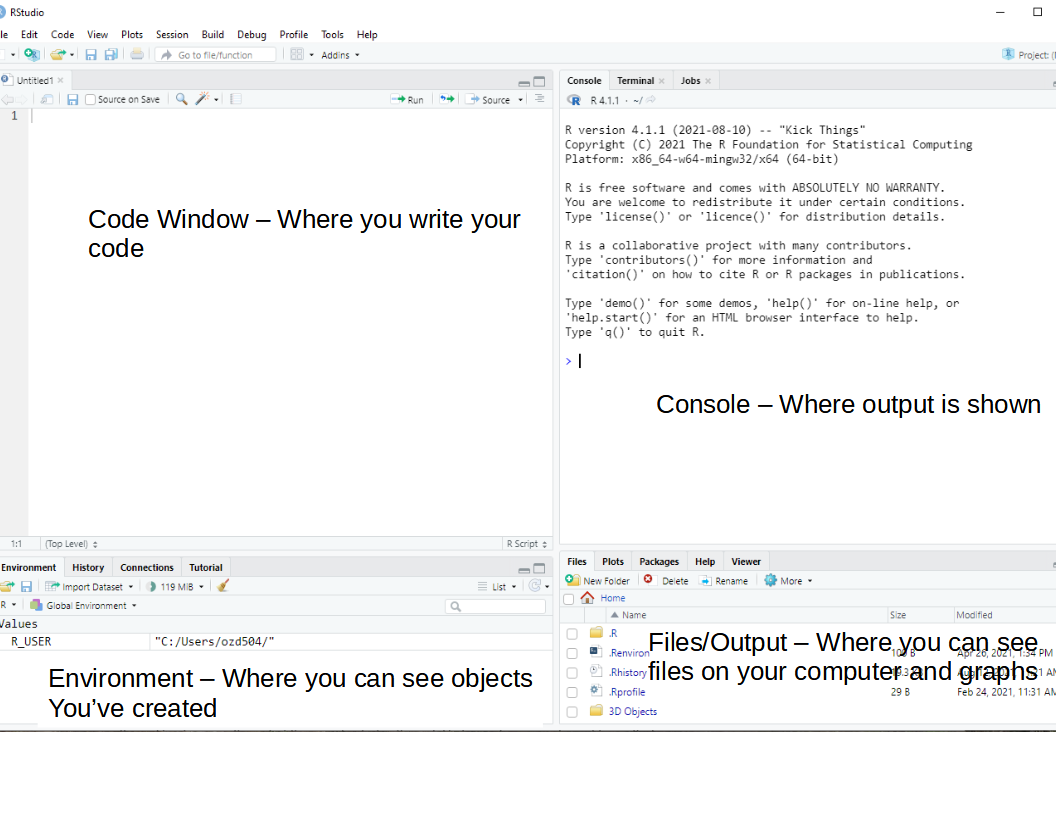
\includegraphics{images/rstudio.png}

\hypertarget{code-windowsource-editor-pane}{%
\subsection{Code window/Source editor
pane}\label{code-windowsource-editor-pane}}

\begin{itemize}
\item
  This is where you write your R code. You can write R code in a few
  different file types (more on this later), but the basic one is an R
  script, with file extension .R
\item
  The code window allows you to write and execute your code one line at
  a time, or to run an entire script at once. I use this to develop new
  code and when I want to test if things work (a VERY common exercise
  when writing any code).
\item
  To run a single line of code, put your cursor on the line and hit
  Ctrl-Enter (on Mac CMD-Enter also does this)
\item
  To run multiple lines of code, highlight the lines you want to run and
  do the same thing
\end{itemize}

\hypertarget{console-pane}{%
\subsection{Console Pane}\label{console-pane}}

\begin{itemize}
\item
  This is where most of your non-graphical output will be shown. Any
  numeric output will appear here, as well as any warnings or error
  messages. In R a warning doesn't necessarily mean something went
  wrong, its just R's polite way of telling you to pay attention.
\item
  An Error means something did go wrong. This is often because you left
  off a ) or a, sometimes because you misspelled something. I routinely
  spell \texttt{length} as \texttt{lenght} which causes R to print an
  error message. If you see an error, don't worry, R will print some
  kind of message telling you what went wrong.
\item
  R's output is in plain text, although we can produce much prettier
  output using other output methods, and we'll talk more about that
  later.
\item
  You can type commands or code into the console as well, and you'll
  immediately get the result, versus if you write it in the Source/Code
  window, you have to run it to see the result. I will often work in the
  console when I want to get ``fast'' answers, meaning little checks
  that I will often do to see the value of something.
\end{itemize}

\hypertarget{environment-or-workspace-browser-pane}{%
\subsection{Environment or Workspace browser
pane}\label{environment-or-workspace-browser-pane}}

\begin{itemize}
\item
  The R environment is where any object you create is stored. In R,
  anything you read in or create with your code is called an object, and
  R is said to be an object oriented programming language.
\item
  Depending on the type of object something is, you may be able to click
  on the object in the environment and see more about it.
\item
  For instance if the object is a data frame, R will open it in a viewer
  where you can explore it like a spreadsheet, and sort and filter it as
  well.
\item
  Other objects may not do anything when you click on them.
\item
  There is also a useful History tab here that shows you recently
  executed lines of code from the console or the code pane.
\end{itemize}

\hypertarget{filesoutputhelp-pane}{%
\subsection{Files/Output/Help pane}\label{filesoutputhelp-pane}}

\begin{itemize}
\item
  The files and output area is where you can interact with files on your
  local computer, such as data files or code files, or images that R can
  open.
\item
  This area also has a plots window that will display plots you create
  in R either via typing directly into the console or by running a
  line(s) of code from the source/code pane.
\item
  There is also a very valuable part of this pane that lets you access
  the help system in R. If you are either looking for something, or you
  just want to explore the functions, you can get access to all of this
  here.
\end{itemize}

\hypertarget{r-file-types}{%
\subsection{R file types}\label{r-file-types}}

\emph{.R files} R uses a basic text file with the .R extension. This
type of file is useful if you're going to write a function or do some
analysis and don't want to have formatted output or text. You can use
these files for everything, but they are limited in their ability to
produce reports and formatted output, so I recommend people work with R
Markdown files instead.

\emph{.Rmd files} Rstudio uses a form of the markdown formatting
language, called R Markdown, for creating formatted documents that
include code, tables, figures and statistical output. \textbf{This book
is written in R Markdown!}

R Markdown is nice for lots of reasons, such as the ability to insert
latex equations into documents.

\[
{y_i \sim Normal (x'\beta, \sigma_2)}
\]

or to include output tables directly into a document:

\begin{Shaded}
\begin{Highlighting}[]
\FunctionTok{library}\NormalTok{(broom)}
\FunctionTok{library}\NormalTok{(pander)}
\NormalTok{fit }\OtherTok{\textless{}{-}} \FunctionTok{lm}\NormalTok{(imr}\SpecialCharTok{\textasciitilde{}}\NormalTok{tfr}\SpecialCharTok{+}\NormalTok{pcturban}\SpecialCharTok{+}\NormalTok{pctlt15\_2018}\SpecialCharTok{+}\NormalTok{pctwomcontra\_all, }
          \AttributeTok{data =}\NormalTok{ prb)}
\FunctionTok{pander}\NormalTok{(broom}\SpecialCharTok{::}\FunctionTok{tidy}\NormalTok{(fit))}
\end{Highlighting}
\end{Shaded}

\begin{longtable}[]{@{}
  >{\centering\arraybackslash}p{(\columnwidth - 8\tabcolsep) * \real{0.2639}}
  >{\centering\arraybackslash}p{(\columnwidth - 8\tabcolsep) * \real{0.1528}}
  >{\centering\arraybackslash}p{(\columnwidth - 8\tabcolsep) * \real{0.1667}}
  >{\centering\arraybackslash}p{(\columnwidth - 8\tabcolsep) * \real{0.1667}}
  >{\centering\arraybackslash}p{(\columnwidth - 8\tabcolsep) * \real{0.1667}}@{}}
\toprule\noalign{}
\begin{minipage}[b]{\linewidth}\centering
term
\end{minipage} & \begin{minipage}[b]{\linewidth}\centering
estimate
\end{minipage} & \begin{minipage}[b]{\linewidth}\centering
std.error
\end{minipage} & \begin{minipage}[b]{\linewidth}\centering
statistic
\end{minipage} & \begin{minipage}[b]{\linewidth}\centering
p.value
\end{minipage} \\
\midrule\noalign{}
\endhead
\bottomrule\noalign{}
\endlastfoot
(Intercept) & 6.209 & 6.551 & 0.9478 & 0.3446 \\
tfr & 3.392 & 2.006 & 1.691 & 0.09274 \\
pcturban & -0.0923 & 0.04553 & -2.028 & 0.04425 \\
pctlt15\_2018 & 0.8699 & 0.2441 & 3.564 & 0.0004798 \\
pctwomcontra\_all & -0.2114 & 0.06018 & -3.512 & 0.0005757 \\
\end{longtable}

This allows you to make tables in Rmarkdown without having to do
non-repeatable tasks in Word or some other program. You can basically do
your entire analysis, or a sideshow for a presentation, or an entire
paper, including bibliography, in Rstudio.

\hypertarget{r-projects}{%
\subsection{R projects}\label{r-projects}}

Rstudio allows you to create a R project, which basically sets up a
specific location to store R code for a given project you may be doing.
For instance, this book is a single R project, which helps me organize
all the chapters, bibliographies, figures, etc.

R projects also allow you to use version control, including Git and SVN,
to collaborate and share code and data with others.

\hypertarget{r-data-files}{%
\subsection{R data files}\label{r-data-files}}

R allows you to read and write its own \emph{native} data formats, as
well as read and write text formatted files and data files from other
statistical software packages. Two native R data formats are
\texttt{.rds} and \texttt{.rdata} formats. \texttt{.rds} files allow you
to save a single R object to an external files, while \texttt{.rdata}
files allow you to save one or more objects to a file.

Here is a short example of doing this, where I create 2 vectors,
\texttt{x} and \texttt{y} and save them.

\begin{Shaded}
\begin{Highlighting}[]
\NormalTok{x }\OtherTok{\textless{}{-}} \FunctionTok{c}\NormalTok{(}\DecValTok{1}\NormalTok{, }\DecValTok{2}\NormalTok{,}\DecValTok{3}\NormalTok{)}

\NormalTok{y }\OtherTok{\textless{}{-}} \FunctionTok{c}\NormalTok{(}\DecValTok{4}\NormalTok{, }\DecValTok{5}\NormalTok{, }\DecValTok{6}\NormalTok{)}

\FunctionTok{saveRDS}\NormalTok{(x, }
        \AttributeTok{file=}\StringTok{"\textasciitilde{}/x.rds"}\NormalTok{)}

\FunctionTok{save}\NormalTok{(}\AttributeTok{list=}\FunctionTok{c}\NormalTok{(}\StringTok{"x"}\NormalTok{,}\StringTok{"y"}\NormalTok{),}
     \AttributeTok{file=}\StringTok{"xy.rdata"}\NormalTok{)}
\end{Highlighting}
\end{Shaded}

I can also load these into R again:

\begin{Shaded}
\begin{Highlighting}[]
\FunctionTok{readRDS}\NormalTok{(}\AttributeTok{file =} \StringTok{"\textasciitilde{}/x.rds"}\NormalTok{)}
\end{Highlighting}
\end{Shaded}

\begin{verbatim}
[1] 1 2 3
\end{verbatim}

\begin{Shaded}
\begin{Highlighting}[]
\FunctionTok{load}\NormalTok{(}\StringTok{"xy.rdata"}\NormalTok{)}
\end{Highlighting}
\end{Shaded}

Standard methods for importing text data such as comma separated value
or tab delimited files can be read into R using \texttt{read.csv()} or
\texttt{read.table()} and similar writing functions are available.

To read in a dataset from another statistical package, I recommend using
the \texttt{haven} package. It allows you to read and write SAS (both
sas7bdat and xpt files), Stata, SPSS (both .por and .sav files).

For example, here I write out a dataframe containing \texttt{x} and
\texttt{y} from above to a SAS version 7 file:

\begin{Shaded}
\begin{Highlighting}[]
\NormalTok{xy }\OtherTok{\textless{}{-}} \FunctionTok{data.frame}\NormalTok{(}\AttributeTok{x =}\NormalTok{ x, }\AttributeTok{y =}\NormalTok{ y)}
\NormalTok{xy}
\end{Highlighting}
\end{Shaded}

\begin{verbatim}
  x y
1 1 4
2 2 5
3 3 6
\end{verbatim}

\begin{Shaded}
\begin{Highlighting}[]
\FunctionTok{library}\NormalTok{(haven)}

\FunctionTok{write\_sas}\NormalTok{(}\AttributeTok{data =}\NormalTok{ xy,}
          \AttributeTok{path =} \StringTok{"\textasciitilde{}/xy.sas7bdat"}\NormalTok{)}
\end{Highlighting}
\end{Shaded}

\begin{verbatim}
Warning: `write_sas()` was deprecated in haven 2.5.2.
i Please use `write_xpt()` instead.
\end{verbatim}

I will describe dataframes more later in the chapter.

R also has packages for reading/writing such data formats as JSON, ESRI
Shapefiles, Excel spreadsheets, Google Spreadsheets, DBF files, in
addition to tools for connecting to SQL databases, and for interfacing
with other statistics packages, such as Mplus, OpenBUGS, WinBUGS and
various Geographic Information Systems.

\hypertarget{getting-help-in-r}{%
\section{Getting help in R}\label{getting-help-in-r}}

I wish I had a nickel for every time I ran into a problem trying to do
something in R, that would be a lot of nickles. Here are some good tips
for finding help in R:

\begin{enumerate}
\def\labelenumi{\arabic{enumi})}
\tightlist
\item
  If you know the name of a function you want to use, but just need help
  using it, try \texttt{?}
\end{enumerate}

\texttt{?lm}

\begin{enumerate}
\def\labelenumi{\arabic{enumi})}
\setcounter{enumi}{1}
\tightlist
\item
  If you need to find a function to do something, try \texttt{??}
\end{enumerate}

\texttt{??"linear\ model"}

\begin{enumerate}
\def\labelenumi{\arabic{enumi})}
\setcounter{enumi}{2}
\tightlist
\item
  You can also search the history of other R users questions by tapping
  into the \href{http://finzi.psych.upenn.edu/search.html}{RSiteSearch}
  website, which is an archive of user questions to the R list serve.
  This can be used by tying \texttt{RSiteSearch()}
\end{enumerate}

\texttt{RSiteSearch("heteroskedasticity")}

\begin{enumerate}
\def\labelenumi{\arabic{enumi})}
\setcounter{enumi}{3}
\item
  Speaking of which, there are multiple
  \href{https://www.r-project.org/mail.html}{R user email list serves}
  that you can ask questions to, or subscribe to daily digests from.
  These typically want an example of what you're trying to do, referred
  to as a \emph{reproducible example}. I wish I also had nickles for
  each question I've asked and answered on these forums.
\item
  A good source for all things programming is the statistics branch of
  \href{https://stats.stackexchange.com}{Stack Exchange}, which has lots
  of contributed questions and answers, although many answers are either
  very snarky or wrong or for an old version of a library, so
  \emph{caveat emptor}.
\item
  Your local R guru or R user group. You would be surprised at how many
  people are R users, there may be one just down the hall, or in the
  cubicle next door. I relish the opportunity to talk to other R users,
  mostly because, even though I've used R for more than 20 years, I
  still learn so much by talking to others about how they use R.
\end{enumerate}

Lastly, I want to be clear that there are often \textbf{more than one
way to do everything} in R. Simple things like reading and writing a CSV
data file can be accomplished by any of a handful of different functions
found in different packages. If someone tells you that there is only one
way to do something, they are usually wrong in such a statement,
regarding R at least.

\hypertarget{r-packages}{%
\section{R packages}\label{r-packages}}

R uses packages to store functions that do different types of analysis,
so we will need to install lots of different packages to do different
things. There are over 20,000 different packages currently for R. These
are hosted on one of a number of \emph{repositories}, such as the
Comprehensive R Archive Network, or CRAN, which is the official
repository for R packages. Other locations where authors store packages
include \href{\%22https://r-forge.r-project.org/\%22}{R-Forge} and
\href{\%22https://www.bioconductor.org/\%22}{BioconductoR}. Many authors
host packages in \href{\%22https://github.com\%22}{Github} repositories,
especially for development purposes.

Packages are often organized into \emph{Task Views}, which CRAN uses to
organize packages into thematic areas. You can find a list of these Task
Views \href{\%22https://cran.r-project.org/web/views/\%22}{here}. There
is not a task view for Demography, but there are ones for the
\href{\%22https://cran.r-project.org/web/views/SocialSciences.html\%22}{Social
Sciences},
\href{\%22https://cran.r-project.org/web/views/Econometrics.html\%22}{Econometrics},
and
\href{\%22https://cran.r-project.org/web/views/Spatial.html\%22}{Spatial
Data} to name a few. Task views allow users to download a lot of
thematically linked packages in a single command, through the package
\texttt{ctv}, or Cran Task Views. You can install this package by
typing:

\texttt{install.packages("ctv")}

into Rstudio. Then you have to load the package by using the
\texttt{library()} command:

\texttt{library(ctv)}

which gives you access to the functions in that package. You don't need
to install the package again, unless you update your R software, but
each time you start a new session (i.e.~open Rstudio), you will have to
load the library again. If you want to install all of the packages in
the Social Science task view, you would type:

\texttt{install.views("SocialSciences")}

into R and it will install all of the packages under that task view, as
of the writing of this sentence, include over 80 packages.

I strongly recommend you install several packages prior to us beginning
to use R, so you will not be distracted by this later. I've written a
short script on my Github repository and you can use it by running:

\begin{Shaded}
\begin{Highlighting}[]
\FunctionTok{source}\NormalTok{(}\StringTok{"https://raw.githubusercontent.com/coreysparks/Rcode/master/install\_first\_short.R"}\NormalTok{)}
\end{Highlighting}
\end{Shaded}

This will install a few dozen R packages that are commonly used for
social science analysis and some other packages I find of use.

You only have to install a package once, but each time you start a R
session, you must load the package to use its functions. You should also
routinely update your installed packages using
\texttt{update.packages(ask\ =\ FALSE)}. This will update any packages
that have new versions on CRAN. These often will contain bug fixes and
new features. On CRAN, each package will have a README file that tells
what has changed in the various versions. Here is one for one of my
favorite packages
\href{https://cran.r-project.org/web/packages/tidycensus/readme/README.html}{\texttt{tidycensus}}.

\hypertarget{functions-within-packages}{%
\subsection{Functions within packages}\label{functions-within-packages}}

Each package will have one or more functions within it, each doing a
specific task. The default way to access all functions within a given
package is to use the command \texttt{library(packagename)} to access
the functions. Once loaded, all the functions will be accessible to you.
Sometimes, different packages have functions with the same name, for
example the base R library has the function \texttt{lag()}, which lag's
a time series, the \texttt{dplyr} library also has a function
\texttt{lag()}, which does a similar task, but with different function
arguments. If you have the \texttt{dplyr} library loaded, R will default
to use its \texttt{lag()} function. If you want to access a specific
function within a specific library, sometimes it is safest to use the
\texttt{library::function()} syntax. So if I want to use base R's
\texttt{lag()} function, I could do

\texttt{stats::lag()}

to access that function specifically. How do you know when this happens?
When you load a library, you will often see messages from R that
functions have conflicts. For example, if I load \texttt{dplyr}, I see:

\begin{figure}

{\centering 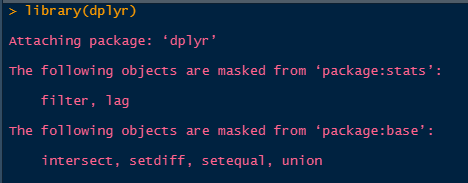
\includegraphics{images/dplyrconflict.png}

}

\caption{Conflict messages}

\end{figure}

As you use R more, you will learn which packages have conflicts, and
often the developers of the packages will do this and rename the
commonly conflicting functions. For example, the function to recode
variables in the \texttt{car} package, \texttt{car::recode()} was
renamed to \texttt{car::Recode()} to avoid conflicts with the
\texttt{dplyr::recode()} function, as both are often used in the same
analysis.

\hypertarget{more-notes-on-functions}{%
\subsubsection{More notes on functions}\label{more-notes-on-functions}}

Functions in R are bits of code that do something, what they do depends
on the code within them. For instance, the \texttt{median()} function's
underlying code can be seen by:

\begin{Shaded}
\begin{Highlighting}[]
\FunctionTok{getAnywhere}\NormalTok{(}\FunctionTok{median.default}\NormalTok{())}
\end{Highlighting}
\end{Shaded}

\begin{verbatim}
A single object matching 'median.default' was found
It was found in the following places
  package:stats
  registered S3 method for median from namespace stats
  namespace:stats
with value

function (x, na.rm = FALSE, ...) 
{
    if (is.factor(x) || is.data.frame(x)) 
        stop("need numeric data")
    if (length(names(x))) 
        names(x) <- NULL
    if (na.rm) 
        x <- x[!is.na(x)]
    else if (any(is.na(x))) 
        return(x[NA_integer_])
    n <- length(x)
    if (n == 0L) 
        return(x[NA_integer_])
    half <- (n + 1L)%/%2L
    if (n%%2L == 1L) 
        sort(x, partial = half)[half]
    else mean(sort(x, partial = half + 0L:1L)[half + 0L:1L])
}
<bytecode: 0x11852ca28>
<environment: namespace:stats>
\end{verbatim}

This seems like a lot, I know, but it allows you to see all of the code
under the hood of any function. Obviously, the more complicated the
function, the more complicated the code. For instance, I can write my
own simple function to find the mean of a sample:

\begin{Shaded}
\begin{Highlighting}[]
\NormalTok{mymean }\OtherTok{\textless{}{-}} \ControlFlowTok{function}\NormalTok{(x,}
                   \AttributeTok{na.rm =} \ConstantTok{FALSE}\NormalTok{)\{}
\NormalTok{  sx }\OtherTok{\textless{}{-}} \FunctionTok{sum}\NormalTok{(x, }
            \AttributeTok{na.rm =} \ConstantTok{FALSE}\NormalTok{)}
\NormalTok{  nx }\OtherTok{\textless{}{-}} \FunctionTok{length}\NormalTok{(x)}
\NormalTok{  mu }\OtherTok{\textless{}{-}}\NormalTok{ sx}\SpecialCharTok{/}\NormalTok{nx}
\NormalTok{  mu}
\NormalTok{\}}

\FunctionTok{mymean}\NormalTok{(}\AttributeTok{x =} \FunctionTok{c}\NormalTok{(}\DecValTok{1}\NormalTok{,}\DecValTok{2}\NormalTok{,}\DecValTok{3}\NormalTok{))}
\end{Highlighting}
\end{Shaded}

\begin{verbatim}
[1] 2
\end{verbatim}

This function only includes the basic machinery to calculate the
arithmetic mean of a vector \(x\). The function has 2
\textbf{arguments}, \texttt{x} and \texttt{na.rm}. All R functions have
one or more arguments that users must enter for the function to operate.
Some arguments are required, while some are optional, also some
arguments, such as the \texttt{na.rm\ =\ FALSE}, have default values. As
mentioned earlier, to see all the information for a function's
arguments, use the help operator, \texttt{?}. For example \texttt{?mean}
will show you the help documents for the \texttt{mean()} function

\begin{figure}

{\centering 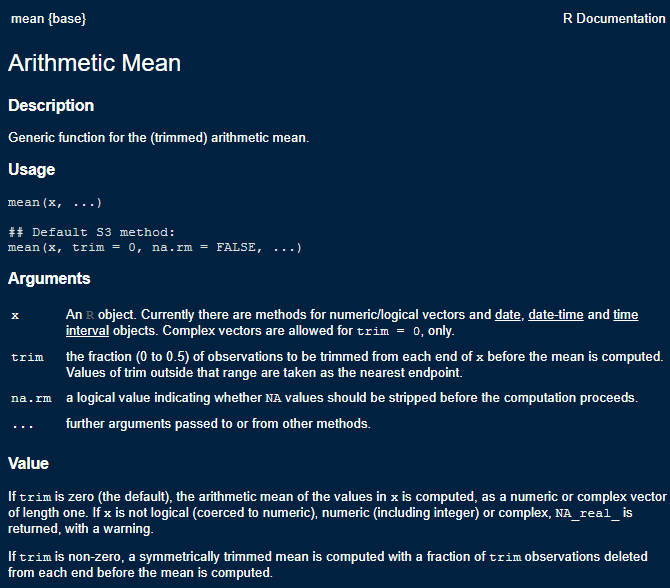
\includegraphics{images/meandoc.png}

}

\caption{Mean Function Help}

\end{figure}

When using a new function, it's always advised to check out the help
file to see all the arguments the function can take, because this is
where you can choose alternative specifications for models and methods.
These help files also contain the original citations for methods, so you
can immediately check the source of the algorithms. The help files also
contain a working example of how to use the function on data contained
in R.

\hypertarget{your-r-user-environment}{%
\section{Your R user environment}\label{your-r-user-environment}}

When you begin an R session (generally by opening Rstudio) you will
begin in your home directory. This is traditionally, on Windows, at
\texttt{\textquotesingle{}C:/Users/yourusername/Documents\textquotesingle{}}
on Mac at
\texttt{\textquotesingle{}/Users/yourusername\textquotesingle{}}, and on
Linux at
\texttt{\textquotesingle{}/users/yourusername\textquotesingle{}}. There
are files you can add to your home directory to specify starting options
for R.

You can find information on setting up \texttt{.Rprofile} and
\texttt{.Renviron} files on
\href{https://cran.r-project.org/web/packages/startup/vignettes/startup-intro.html}{CRAN's
website}. This allows you to setup packages that load every time R
starts, to save API keys and other various options. These are completely
optional and many R users never touch these.

If you're not sure where you are you can type \texttt{getwd()}, for get
working directory, and R will tell you:

\begin{Shaded}
\begin{Highlighting}[]
\FunctionTok{getwd}\NormalTok{()}
\end{Highlighting}
\end{Shaded}

If you don't like where you start, you can change it, by using
\texttt{setwd()}, to set your working directory to a new location.

\begin{Shaded}
\begin{Highlighting}[]
\FunctionTok{setwd}\NormalTok{(}\StringTok{"\textasciitilde{}"}\NormalTok{)}
\FunctionTok{getwd}\NormalTok{()}
\end{Highlighting}
\end{Shaded}

R projects will typically set the home folder for the project at the
directory location of the project, so files associate with the project
will always be in the same place. You can set this at the beginning of
your R code file to ensure the code will look for data in a specific
location.

\hypertarget{some-simple-r-examples}{%
\section{Some Simple R examples}\label{some-simple-r-examples}}

Below we will go through a simple R session where we introduce some
concepts that are important for R. I'm running these in an Rstudio
session, in the

\hypertarget{r-is-a-calculator}{%
\subsection{R is a calculator}\label{r-is-a-calculator}}

\begin{Shaded}
\begin{Highlighting}[]
\CommentTok{\#addition and subtraction}
\DecValTok{3}\SpecialCharTok{+}\DecValTok{7}
\end{Highlighting}
\end{Shaded}

\begin{verbatim}
[1] 10
\end{verbatim}

\begin{Shaded}
\begin{Highlighting}[]
\DecValTok{3{-}7}
\end{Highlighting}
\end{Shaded}

\begin{verbatim}
[1] -4
\end{verbatim}

\begin{Shaded}
\begin{Highlighting}[]
\CommentTok{\#multiplication and division}
\DecValTok{3}\SpecialCharTok{*}\DecValTok{7}
\end{Highlighting}
\end{Shaded}

\begin{verbatim}
[1] 21
\end{verbatim}

\begin{Shaded}
\begin{Highlighting}[]
\DecValTok{3}\SpecialCharTok{/}\DecValTok{7}
\end{Highlighting}
\end{Shaded}

\begin{verbatim}
[1] 0.4285714
\end{verbatim}

\begin{Shaded}
\begin{Highlighting}[]
\CommentTok{\#powers}
\DecValTok{3}\SpecialCharTok{\^{}}\DecValTok{2}
\end{Highlighting}
\end{Shaded}

\begin{verbatim}
[1] 9
\end{verbatim}

\begin{Shaded}
\begin{Highlighting}[]
\DecValTok{3}\SpecialCharTok{\^{}}\DecValTok{3}
\end{Highlighting}
\end{Shaded}

\begin{verbatim}
[1] 27
\end{verbatim}

\begin{Shaded}
\begin{Highlighting}[]
\CommentTok{\#common math functions}
\FunctionTok{log}\NormalTok{(}\DecValTok{3}\SpecialCharTok{/}\DecValTok{7}\NormalTok{)}
\end{Highlighting}
\end{Shaded}

\begin{verbatim}
[1] -0.8472979
\end{verbatim}

\begin{Shaded}
\begin{Highlighting}[]
\FunctionTok{exp}\NormalTok{(}\DecValTok{3}\SpecialCharTok{/}\DecValTok{7}\NormalTok{)}
\end{Highlighting}
\end{Shaded}

\begin{verbatim}
[1] 1.535063
\end{verbatim}

\begin{Shaded}
\begin{Highlighting}[]
\FunctionTok{sin}\NormalTok{(}\DecValTok{3}\SpecialCharTok{/}\DecValTok{7}\NormalTok{)}
\end{Highlighting}
\end{Shaded}

\begin{verbatim}
[1] 0.4155719
\end{verbatim}

R allows users to write custom functions as well. In general, if you
find yourself writing the same code over and over again, you should
probably just write a function and save it to your local user
environment.

For example a very simple function is given below, it takes a variable
\(x\) as an argument, and then exponentiates the value of the variable.

\begin{Shaded}
\begin{Highlighting}[]
\CommentTok{\#custom functions}
\NormalTok{myfun }\OtherTok{\textless{}{-}} \ControlFlowTok{function}\NormalTok{(x)\{}
  \FunctionTok{exp}\NormalTok{(x)}
\NormalTok{\}}

\FunctionTok{myfun}\NormalTok{(.}\DecValTok{5}\NormalTok{)}
\end{Highlighting}
\end{Shaded}

\begin{verbatim}
[1] 1.648721
\end{verbatim}

\begin{Shaded}
\begin{Highlighting}[]
\FunctionTok{myfun}\NormalTok{(}\SpecialCharTok{{-}}\NormalTok{.}\DecValTok{1}\NormalTok{)}
\end{Highlighting}
\end{Shaded}

\begin{verbatim}
[1] 0.9048374
\end{verbatim}

You may want to save this function for future use, so you don't have to
write it over again. In general, this is why people write R packages, to
store custom functions, but you can also save the function to an R
script. One such way to do this is to use the \texttt{dump()} command.

\begin{Shaded}
\begin{Highlighting}[]
\FunctionTok{dump}\NormalTok{(}\StringTok{"myfun"}\NormalTok{, }
     \AttributeTok{file=}\StringTok{"myfun1.R"}\NormalTok{)}
\end{Highlighting}
\end{Shaded}

One way to load this function when you want to use it is to use the
\texttt{source()} command, which loads any code in a given R script.

\begin{Shaded}
\begin{Highlighting}[]
\FunctionTok{source}\NormalTok{(}\StringTok{"myfun1.R"}\NormalTok{)}
\end{Highlighting}
\end{Shaded}

Which will load this function into your local environment and you can
use it. If you are interested in writing your own packages, I would
highly recommend reading Wickham (n.d.).

\hypertarget{variables-and-objects}{%
\section{Variables and objects}\label{variables-and-objects}}

In R we assign values to objects (object-oriented programming). These
can generally have any name, but some names are reserved for R. For
instance you probably wouldn't want to call something `mean' because
there's a `mean()' function already in R. For instance:

\begin{Shaded}
\begin{Highlighting}[]
\NormalTok{x }\OtherTok{\textless{}{-}} \DecValTok{3}
\NormalTok{y }\OtherTok{\textless{}{-}} \DecValTok{7}
\NormalTok{x}\SpecialCharTok{+}\NormalTok{y}
\end{Highlighting}
\end{Shaded}

\begin{verbatim}
[1] 10
\end{verbatim}

\begin{Shaded}
\begin{Highlighting}[]
\NormalTok{x}\SpecialCharTok{*}\NormalTok{y}
\end{Highlighting}
\end{Shaded}

\begin{verbatim}
[1] 21
\end{verbatim}

\begin{Shaded}
\begin{Highlighting}[]
\FunctionTok{log}\NormalTok{(x}\SpecialCharTok{*}\NormalTok{y)}
\end{Highlighting}
\end{Shaded}

\begin{verbatim}
[1] 3.044522
\end{verbatim}

The \texttt{{[}1{]}} in the answer refers to the first element of a
\emph{vector}, which brings us to\ldots{}

\hypertarget{vectors}{%
\subsection{Vectors}\label{vectors}}

R thinks many objects are like a matrix, or a vector, meaning a row or
column that contains either numbers or characters. One of R's big
selling points is that much of it is completely vectorized. Meaning, I
can apply an operation along all elements of a vector without having to
write a \emph{loop}.

For example, if I want to multiply a vector of numbers by a constant, in
SAS, I could do:

\texttt{for\ (i\ in\ 1\ to\ 5)}
\texttt{x{[}i{]}\ \textless{}-\ y{[}i{]}*5} \texttt{end;}

but in R, I can just do:

\begin{Shaded}
\begin{Highlighting}[]
\NormalTok{x }\OtherTok{\textless{}{-}} \FunctionTok{c}\NormalTok{(}\DecValTok{3}\NormalTok{, }\DecValTok{4}\NormalTok{, }\DecValTok{5}\NormalTok{, }\DecValTok{6}\NormalTok{, }\DecValTok{7}\NormalTok{)}
\CommentTok{\#c() makes a vector}
\NormalTok{y }\OtherTok{\textless{}{-}} \DecValTok{7}

\NormalTok{x}\SpecialCharTok{*}\NormalTok{y}
\end{Highlighting}
\end{Shaded}

\begin{verbatim}
[1] 21 28 35 42 49
\end{verbatim}

R is also very good about using vectors, let's say I wanted to find the
third element of x:

\begin{Shaded}
\begin{Highlighting}[]
\NormalTok{x[}\DecValTok{3}\NormalTok{]}
\end{Highlighting}
\end{Shaded}

\begin{verbatim}
[1] 5
\end{verbatim}

or if I want to test if this element is 10

\begin{Shaded}
\begin{Highlighting}[]
\NormalTok{x[}\DecValTok{3}\NormalTok{] }\SpecialCharTok{==} \DecValTok{10}
\end{Highlighting}
\end{Shaded}

\begin{verbatim}
[1] FALSE
\end{verbatim}

\begin{Shaded}
\begin{Highlighting}[]
\NormalTok{x[}\DecValTok{3}\NormalTok{] }\SpecialCharTok{!=} \DecValTok{10}
\end{Highlighting}
\end{Shaded}

\begin{verbatim}
[1] TRUE
\end{verbatim}

or is it larger than another number:

\begin{Shaded}
\begin{Highlighting}[]
\NormalTok{x[}\DecValTok{3}\NormalTok{] }\SpecialCharTok{\textgreater{}} \DecValTok{3}
\end{Highlighting}
\end{Shaded}

\begin{verbatim}
[1] TRUE
\end{verbatim}

or is any element of the whole vector greater than 3

\begin{Shaded}
\begin{Highlighting}[]
\NormalTok{x }\SpecialCharTok{\textgreater{}} \DecValTok{3}
\end{Highlighting}
\end{Shaded}

\begin{verbatim}
[1] FALSE  TRUE  TRUE  TRUE  TRUE
\end{verbatim}

If you want to see what's in an object, use \texttt{str()}, for
\texttt{str}ucture

\begin{Shaded}
\begin{Highlighting}[]
\FunctionTok{str}\NormalTok{(x)}
\end{Highlighting}
\end{Shaded}

\begin{verbatim}
 num [1:5] 3 4 5 6 7
\end{verbatim}

and we see that x is numeric, and has the values that we made.

We can also see different characteristics of x

\begin{Shaded}
\begin{Highlighting}[]
\CommentTok{\#how long is x?}
\FunctionTok{length}\NormalTok{(x)}
\end{Highlighting}
\end{Shaded}

\begin{verbatim}
[1] 5
\end{verbatim}

\begin{Shaded}
\begin{Highlighting}[]
\CommentTok{\#is x numeric?}
\FunctionTok{is.numeric}\NormalTok{(x)}
\end{Highlighting}
\end{Shaded}

\begin{verbatim}
[1] TRUE
\end{verbatim}

\begin{Shaded}
\begin{Highlighting}[]
\CommentTok{\#is x full of characters?}
\FunctionTok{is.character}\NormalTok{(x)}
\end{Highlighting}
\end{Shaded}

\begin{verbatim}
[1] FALSE
\end{verbatim}

\begin{Shaded}
\begin{Highlighting}[]
\CommentTok{\#is any element of x missing?}
\FunctionTok{is.na}\NormalTok{(x)}
\end{Highlighting}
\end{Shaded}

\begin{verbatim}
[1] FALSE FALSE FALSE FALSE FALSE
\end{verbatim}

\begin{Shaded}
\begin{Highlighting}[]
\CommentTok{\#now i\textquotesingle{}ll modify x}
\NormalTok{x }\OtherTok{\textless{}{-}} \FunctionTok{c}\NormalTok{(x, }\ConstantTok{NA}\NormalTok{) }\CommentTok{\#combine x and a missing value ==NA}
\NormalTok{x}
\end{Highlighting}
\end{Shaded}

\begin{verbatim}
[1]  3  4  5  6  7 NA
\end{verbatim}

\begin{Shaded}
\begin{Highlighting}[]
\CommentTok{\#Now ask if any x\textquotesingle{}s are missing}
\FunctionTok{is.na}\NormalTok{(x)}
\end{Highlighting}
\end{Shaded}

\begin{verbatim}
[1] FALSE FALSE FALSE FALSE FALSE  TRUE
\end{verbatim}

\hypertarget{replacing-elements-of-vectors}{%
\subsubsection{Replacing elements of
vectors}\label{replacing-elements-of-vectors}}

Above, we had a missing value in X, let's say we want to replace it with
another value. He we will use basic conditional logic, which exists in
any programming language. The \texttt{ifelse()} function will evaluate a
\texttt{test} statement, and depending on if that statement is true, it
will assign a value, if the statement is false, R will assign another
value. Here, we replace the missing value with \(\sqrt{7.2}\), and leave
the other values as they are.

\begin{Shaded}
\begin{Highlighting}[]
\NormalTok{x }\OtherTok{\textless{}{-}} \FunctionTok{ifelse}\NormalTok{(}\AttributeTok{test =} \FunctionTok{is.na}\NormalTok{(x) }\SpecialCharTok{==} \ConstantTok{TRUE}\NormalTok{,}
            \AttributeTok{yes =}  \FunctionTok{sqrt}\NormalTok{(}\FloatTok{7.2}\NormalTok{),}
            \AttributeTok{no =}\NormalTok{  x)}
\NormalTok{x}
\end{Highlighting}
\end{Shaded}

\begin{verbatim}
[1] 3.000000 4.000000 5.000000 6.000000 7.000000 2.683282
\end{verbatim}

\hypertarget{variable-types}{%
\section{Variable types}\label{variable-types}}

R stores data differently depending on the type of information
contained. Common variables types in R are numeric, character, integer
and factor.

Numeric variables are just that, numbers. They can be whole numbers or
decimal values. The best way to see if a variable is numeric is to use
\texttt{is.numeric(x)}, and R will return TRUE if the variable is
numeric and FALSE if it is not.

\begin{Shaded}
\begin{Highlighting}[]
\FunctionTok{is.numeric}\NormalTok{(x)}
\end{Highlighting}
\end{Shaded}

\begin{verbatim}
[1] TRUE
\end{verbatim}

Likewise, you can use \texttt{is.character()}, \texttt{is.integer()},
and \texttt{is.factor} to identify if a variable is of a given type. The
\texttt{class()} function will also do this more generally:

\begin{Shaded}
\begin{Highlighting}[]
\FunctionTok{class}\NormalTok{(x)}
\end{Highlighting}
\end{Shaded}

\begin{verbatim}
[1] "numeric"
\end{verbatim}

Character and factor variables often store the same kind of information,
and R (until recently) would always convert character variables to
factors when data were read into R. This is the option
\texttt{getOption("stringsAsFactors")}, which used to default to True,
but has recently changed. What's the difference you ask? Character
variables store information on strings, or text. This is one way to code
categorical variables that are strings. Factors, on the other hand can
store strings OR numbers as categorical variables, and can be ordered or
unordered. Factors also allow for specific categories of the variable to
be considered as reference categories, as are often used in many
statistical procedures. Factor variables have ``levels'' which are the
different values of the categorical variable, this implied a more
complicated structure than simple character variables, which lack these
qualities.

You can manipulate variables of one type into another, with some notable
things to watch out for.

Here are some examples:

\begin{Shaded}
\begin{Highlighting}[]
\CommentTok{\#create at numeric vector}

\NormalTok{z }\OtherTok{\textless{}{-}}  \FunctionTok{c}\NormalTok{(}\DecValTok{1}\NormalTok{,}\DecValTok{2}\NormalTok{,}\DecValTok{3}\NormalTok{,}\DecValTok{4}\NormalTok{)}
\FunctionTok{class}\NormalTok{(z)}
\end{Highlighting}
\end{Shaded}

\begin{verbatim}
[1] "numeric"
\end{verbatim}

We can convert this to a character vector using \texttt{as.character()}

\begin{Shaded}
\begin{Highlighting}[]
\NormalTok{zc }\OtherTok{\textless{}{-}}  \FunctionTok{as.character}\NormalTok{(z)}
\NormalTok{zc}
\end{Highlighting}
\end{Shaded}

\begin{verbatim}
[1] "1" "2" "3" "4"
\end{verbatim}

Likewise, we can convert it to a factor type:

\begin{Shaded}
\begin{Highlighting}[]
\NormalTok{zf }\OtherTok{\textless{}{-}} \FunctionTok{as.factor}\NormalTok{(z)}
\NormalTok{zf}
\end{Highlighting}
\end{Shaded}

\begin{verbatim}
[1] 1 2 3 4
Levels: 1 2 3 4
\end{verbatim}

\begin{Shaded}
\begin{Highlighting}[]
\FunctionTok{class}\NormalTok{(zf)}
\end{Highlighting}
\end{Shaded}

\begin{verbatim}
[1] "factor"
\end{verbatim}

\begin{Shaded}
\begin{Highlighting}[]
\FunctionTok{is.ordered}\NormalTok{(zf)}
\end{Highlighting}
\end{Shaded}

\begin{verbatim}
[1] FALSE
\end{verbatim}

and as an ordered factor:

\begin{Shaded}
\begin{Highlighting}[]
\NormalTok{zfo }\OtherTok{\textless{}{-}} \FunctionTok{factor}\NormalTok{(zf, }
              \AttributeTok{ordered =} \ConstantTok{TRUE}\NormalTok{)}
\NormalTok{zfo}
\end{Highlighting}
\end{Shaded}

\begin{verbatim}
[1] 1 2 3 4
Levels: 1 < 2 < 3 < 4
\end{verbatim}

Another very useful variable type is the \emph{logical} type. In R a
logical variable is either a \texttt{TRUE} or \texttt{FALSE} value. I
personally use this a lot in my work in both preliminary data analysis
and data checking. We saw this used above, when we did
\texttt{is.na(x)\ ==\ TRUE} to check if the \texttt{x} variable was
missing. We can see how this translates into a logical variable here:

\begin{Shaded}
\begin{Highlighting}[]
\NormalTok{x }\OtherTok{\textless{}{-}} \FunctionTok{c}\NormalTok{(}\DecValTok{3}\NormalTok{, }\DecValTok{4}\NormalTok{, }\DecValTok{5}\NormalTok{, }\DecValTok{6}\NormalTok{, }\DecValTok{7}\NormalTok{, }\ConstantTok{NA}\NormalTok{)}

\NormalTok{z}\OtherTok{\textless{}{-}}\FunctionTok{is.na}\NormalTok{(x) }\CommentTok{\#check if x is missing}

\NormalTok{z}
\end{Highlighting}
\end{Shaded}

\begin{verbatim}
[1] FALSE FALSE FALSE FALSE FALSE  TRUE
\end{verbatim}

\begin{Shaded}
\begin{Highlighting}[]
\FunctionTok{class}\NormalTok{(z)}
\end{Highlighting}
\end{Shaded}

\begin{verbatim}
[1] "logical"
\end{verbatim}

In practice, I use this with the \texttt{I()} function (more on this
below) to do quick binary codes of a value:

\begin{Shaded}
\begin{Highlighting}[]
\NormalTok{x }\OtherTok{\textless{}{-}} \FunctionTok{c}\NormalTok{(}\DecValTok{3}\NormalTok{, }\DecValTok{4}\NormalTok{, }\DecValTok{5}\NormalTok{, }\DecValTok{6}\NormalTok{, }\DecValTok{7}\NormalTok{)}

\FunctionTok{table}\NormalTok{( }\FunctionTok{I}\NormalTok{(x }\SpecialCharTok{\textgreater{}=} \DecValTok{5}\NormalTok{) )}
\end{Highlighting}
\end{Shaded}

\begin{verbatim}

FALSE  TRUE 
    2     3 
\end{verbatim}

\hypertarget{dataframes}{%
\section{Dataframes}\label{dataframes}}

Traditionally, R organizes variables into data frames, these are like a
spreadsheet. The columns can have names, and the \emph{dataframe} itself
can have data of different types.

Here we make a short data frame with three columns, two numeric and one
factor:

\begin{Shaded}
\begin{Highlighting}[]
\NormalTok{mydat }\OtherTok{\textless{}{-}} \FunctionTok{data.frame}\NormalTok{(}
  \AttributeTok{x =} \FunctionTok{c}\NormalTok{(}\DecValTok{1}\NormalTok{,}\DecValTok{2}\NormalTok{,}\DecValTok{3}\NormalTok{,}\DecValTok{4}\NormalTok{,}\DecValTok{5}\NormalTok{, }\DecValTok{6}\NormalTok{, }\DecValTok{7}\NormalTok{, }\DecValTok{8}\NormalTok{),}
  \AttributeTok{y =} \FunctionTok{c}\NormalTok{(}\DecValTok{10}\NormalTok{, }\DecValTok{20}\NormalTok{, }\DecValTok{35}\NormalTok{, }\DecValTok{57}\NormalTok{, }\DecValTok{37}\NormalTok{, }\DecValTok{21}\NormalTok{, }\DecValTok{23}\NormalTok{, }\DecValTok{25}\NormalTok{),}
  \AttributeTok{group =} \FunctionTok{factor}\NormalTok{(}\FunctionTok{c}\NormalTok{(}\StringTok{"A"}\NormalTok{, }\StringTok{"A"}\NormalTok{ ,}\StringTok{"A"}\NormalTok{, }\StringTok{"B"}\NormalTok{, }\StringTok{"B"}\NormalTok{, }\StringTok{"C"}\NormalTok{,}\StringTok{"C"}\NormalTok{,}\StringTok{"C"}\NormalTok{))}
\NormalTok{)}

\CommentTok{\#See the size of the dataframe}
\FunctionTok{dim}\NormalTok{(mydat)}
\end{Highlighting}
\end{Shaded}

\begin{verbatim}
[1] 8 3
\end{verbatim}

\begin{Shaded}
\begin{Highlighting}[]
\CommentTok{\#Open the dataframe in a viewer and just print it}
\FunctionTok{print}\NormalTok{(mydat)}
\end{Highlighting}
\end{Shaded}

\begin{verbatim}
  x  y group
1 1 10     A
2 2 20     A
3 3 35     A
4 4 57     B
5 5 37     B
6 6 21     C
7 7 23     C
8 8 25     C
\end{verbatim}

\hypertarget{accessing-variables-in-dataframes}{%
\subsection{Accessing variables in
dataframes}\label{accessing-variables-in-dataframes}}

R has a few different ways to get a variable from a data set. One way is
the \texttt{\$} notation, used like \texttt{dataset\$variable}, and
another is to provide the column index or name of the variable. These
three methods are illustrated below. The first tells R to get the
variable named \texttt{group} from the data. The second tells R to get
the column named \texttt{group} from the data, and the third tells R to
get the third column from the data.

\begin{Shaded}
\begin{Highlighting}[]
\NormalTok{mydat}\SpecialCharTok{$}\NormalTok{group}
\end{Highlighting}
\end{Shaded}

\begin{verbatim}
[1] A A A B B C C C
Levels: A B C
\end{verbatim}

\begin{Shaded}
\begin{Highlighting}[]
\NormalTok{mydat[}\StringTok{\textquotesingle{}group\textquotesingle{}}\NormalTok{] }
\end{Highlighting}
\end{Shaded}

\begin{verbatim}
  group
1     A
2     A
3     A
4     B
5     B
6     C
7     C
8     C
\end{verbatim}

\begin{Shaded}
\begin{Highlighting}[]
\NormalTok{mydat[,}\DecValTok{3}\NormalTok{]}
\end{Highlighting}
\end{Shaded}

\begin{verbatim}
[1] A A A B B C C C
Levels: A B C
\end{verbatim}

The \texttt{names()} function is very useful for seeing all the column
names of a dataset, without having to print any of the data.

\begin{Shaded}
\begin{Highlighting}[]
\FunctionTok{names}\NormalTok{(mydat)}
\end{Highlighting}
\end{Shaded}

\begin{verbatim}
[1] "x"     "y"     "group"
\end{verbatim}

R has several useful function for previewing the contents of a dataframe
or variable. The \texttt{head()} function shows the first 6 observations
of a dataframe or variable, and \texttt{tail()} shows the last 6
observations. You can also show a custom number of observations by using
the \texttt{n=} argument in either function. These are illustrated
below:

\begin{Shaded}
\begin{Highlighting}[]
\FunctionTok{head}\NormalTok{(mydat)}
\end{Highlighting}
\end{Shaded}

\begin{verbatim}
  x  y group
1 1 10     A
2 2 20     A
3 3 35     A
4 4 57     B
5 5 37     B
6 6 21     C
\end{verbatim}

\begin{Shaded}
\begin{Highlighting}[]
\FunctionTok{head}\NormalTok{(mydat, }\AttributeTok{n =} \DecValTok{2}\NormalTok{)}
\end{Highlighting}
\end{Shaded}

\begin{verbatim}
  x  y group
1 1 10     A
2 2 20     A
\end{verbatim}

\begin{Shaded}
\begin{Highlighting}[]
\FunctionTok{head}\NormalTok{(mydat}\SpecialCharTok{$}\NormalTok{group)}
\end{Highlighting}
\end{Shaded}

\begin{verbatim}
[1] A A A B B C
Levels: A B C
\end{verbatim}

\begin{Shaded}
\begin{Highlighting}[]
\FunctionTok{tail}\NormalTok{(mydat)}
\end{Highlighting}
\end{Shaded}

\begin{verbatim}
  x  y group
3 3 35     A
4 4 57     B
5 5 37     B
6 6 21     C
7 7 23     C
8 8 25     C
\end{verbatim}

\begin{Shaded}
\begin{Highlighting}[]
\FunctionTok{tail}\NormalTok{(mydat, }\AttributeTok{n =} \DecValTok{2}\NormalTok{)}
\end{Highlighting}
\end{Shaded}

\begin{verbatim}
  x  y group
7 7 23     C
8 8 25     C
\end{verbatim}

\begin{Shaded}
\begin{Highlighting}[]
\FunctionTok{tail}\NormalTok{(mydat}\SpecialCharTok{$}\NormalTok{group)}
\end{Highlighting}
\end{Shaded}

\begin{verbatim}
[1] A B B C C C
Levels: A B C
\end{verbatim}

\hypertarget{nicer-looking-tables}{%
\subsection{Nicer looking tables}\label{nicer-looking-tables}}

R can also produce nicely formatted HTML and LaTeX tables. There are
several packages that do this, but the \texttt{knitr} package has some
basic table creation functions that do a good job for simple tables.

\begin{Shaded}
\begin{Highlighting}[]
\FunctionTok{library}\NormalTok{(knitr)}

\FunctionTok{kable}\NormalTok{(mydat,}
      \AttributeTok{caption =} \StringTok{"My basic table"}\NormalTok{,}
      \AttributeTok{align =} \StringTok{\textquotesingle{}c\textquotesingle{}}\NormalTok{,  }
      \AttributeTok{format =} \StringTok{"html"}\NormalTok{)}
\end{Highlighting}
\end{Shaded}

\begin{Shaded}
\begin{Highlighting}[]
\FunctionTok{library}\NormalTok{(knitr)}
\FunctionTok{kable}\NormalTok{(mydat,}
      \AttributeTok{caption =} \StringTok{"My basic table"}\NormalTok{,}
      \AttributeTok{align =} \StringTok{\textquotesingle{}c\textquotesingle{}}\NormalTok{,  }
      \AttributeTok{format=}\StringTok{"latex"}\NormalTok{  )}
\end{Highlighting}
\end{Shaded}

\begin{table}

\caption{My basic table}
\centering
\begin{tabular}[t]{c|c|c}
\hline
x & y & group\\
\hline
1 & 10 & A\\
\hline
2 & 20 & A\\
\hline
3 & 35 & A\\
\hline
4 & 57 & B\\
\hline
5 & 37 & B\\
\hline
6 & 21 & C\\
\hline
7 & 23 & C\\
\hline
8 & 25 & C\\
\hline
\end{tabular}
\end{table}

Much more advanced tables can be created using the \texttt{gt} package
Iannone, Cheng, and Schloerke (2020), which allows for highly customized
tables.

\begin{Shaded}
\begin{Highlighting}[]
\FunctionTok{library}\NormalTok{(gt, }
        \AttributeTok{quietly =} \ConstantTok{TRUE}\NormalTok{)}
\FunctionTok{library}\NormalTok{(dplyr,}
        \AttributeTok{quietly =} \ConstantTok{TRUE}\NormalTok{)}
\end{Highlighting}
\end{Shaded}

\begin{verbatim}

Attaching package: 'dplyr'
\end{verbatim}

\begin{verbatim}
The following objects are masked from 'package:stats':

    filter, lag
\end{verbatim}

\begin{verbatim}
The following objects are masked from 'package:base':

    intersect, setdiff, setequal, union
\end{verbatim}

\begin{Shaded}
\begin{Highlighting}[]
\NormalTok{mydat}\SpecialCharTok{\%\textgreater{}\%}
  \FunctionTok{gt}\NormalTok{()}\SpecialCharTok{\%\textgreater{}\%}
  \FunctionTok{tab\_header}\NormalTok{(}\AttributeTok{title=} \StringTok{"My simple gt table"}\NormalTok{,}
             \AttributeTok{subtitle =} \StringTok{"With a subtitle"}\NormalTok{)}
\end{Highlighting}
\end{Shaded}

\begin{longtable*}{rrc}
\caption*{
{\large My simple gt table} \\ 
{\small With a subtitle}
} \\ 
\toprule
x & y & group \\ 
\midrule
1 & 10 & A \\ 
2 & 20 & A \\ 
3 & 35 & A \\ 
4 & 57 & B \\ 
5 & 37 & B \\ 
6 & 21 & C \\ 
7 & 23 & C \\ 
8 & 25 & C \\ 
\bottomrule
\end{longtable*}

\hypertarget{real-data-example}{%
\section{Real data example}\label{real-data-example}}

Now let's open a `real' data file. This is the
\href{https://www.prb.org/2018-world-population-data-sheet-with-focus-on-changing-age-structures/}{2018
World population data sheet} from the
\href{http://www.prb.org}{Population Reference Bureau}. It contains
summary information on many demographic and population level
characteristics of nations around the world in 2018.

I've had this entered into a \textbf{Comma Separated Values} file by
some poor previous research assistant of mine and it lives happily on
Github now for all the world to see. CSV files are a good way to store
data coming out of a spreadsheet, because R can read them without any
other packages. R can also read Excel files, but it requires external
packages to do so, such as \texttt{readxl}.

I can read it from Github directly by using a function in the
\texttt{readr} library, or with the base R function \texttt{read.csv()},
both accomplish the same task.

\begin{Shaded}
\begin{Highlighting}[]
\NormalTok{prb }\OtherTok{\textless{}{-}} \FunctionTok{read.csv}\NormalTok{(}\AttributeTok{file =} \StringTok{"https://github.com/coreysparks/r\_courses/raw/master/data/2018\_WPDS\_Data\_Table\_FINAL.csv"}\NormalTok{,}
    \AttributeTok{stringsAsFactors =} \ConstantTok{TRUE}\NormalTok{)}
\end{Highlighting}
\end{Shaded}

That's handy. If the file lived on our computer in your working
directory, I could read it in like so:

\begin{Shaded}
\begin{Highlighting}[]
\NormalTok{prb }\OtherTok{\textless{}{-}} \FunctionTok{read\_csv}\NormalTok{(}\StringTok{"path/to/file/2018\_WPDS\_Data\_Table\_FINAL.csv"}\NormalTok{)}
\end{Highlighting}
\end{Shaded}

Same result.

The \texttt{haven} library Wickham and Miller (2020) can read files from
other statistical packages easily, so if you have data in Stata, SAS or
SPSS, you can read it into R using those functions, for example, the
\texttt{read\_dta()} function reads Stata files, \texttt{read\_sav()} to
read SPSS data files.

\begin{Shaded}
\begin{Highlighting}[]
\FunctionTok{library}\NormalTok{(haven)}
\NormalTok{prb\_stata }\OtherTok{\textless{}{-}} \FunctionTok{read\_dta}\NormalTok{(}\StringTok{"path/to/file/prb2018.dta"}\NormalTok{)}

\NormalTok{prb\_spss }\OtherTok{\textless{}{-}} \FunctionTok{read\_sav}\NormalTok{(}\StringTok{"path/to/file/prb\_2018.sav"}\NormalTok{)}
\end{Highlighting}
\end{Shaded}

\hypertarget{basic-descriptive-analysis-of-data}{%
\section{Basic Descriptive analysis of
data}\label{basic-descriptive-analysis-of-data}}

One of the key elements of analyzing data is the initial descriptive
analysis of it. In subsequent chapters, I will go into more depth about
this process, but for now, I want to illustrate some simple but
effective commands for summarizing data.

\hypertarget{dataframe-summaries}{%
\subsection{Dataframe summaries}\label{dataframe-summaries}}

The \texttt{summary()} function is very useful both in terms of
producing numerical summaries of individual variables, but also for
shows summaries of entire dataframes. Its output differs based on the
type of variable you give it, for character variables it does not return
any summary. For factor variables, it returns a frequency table, and for
numeric variables, it returns the five number summary plus the mean.

\begin{Shaded}
\begin{Highlighting}[]
\FunctionTok{summary}\NormalTok{(prb}\SpecialCharTok{$}\NormalTok{region)}
\end{Highlighting}
\end{Shaded}

\begin{verbatim}
       CARIBBEAN  CENTRAL AMERICA     CENTRAL ASIA        EAST ASIA 
              17                8                5                8 
  EASTERN AFRICA   EASTERN EUROPE    MIDDLE AFRICA  NORTHERN AFRICA 
              20               10                9                7 
NORTHERN AMERICA  NORTHERN EUROPE          OCEANIA    SOUTH AMERICA 
               2               11               17               13 
      SOUTH ASIA   SOUTHEAST ASIA  SOUTHERN AFRICA  SOUTHERN EUROPE 
               9               11                5               15 
  WESTERN AFRICA     WESTERN ASIA   WESTERN EUROPE 
              16               18                9 
\end{verbatim}

\begin{Shaded}
\begin{Highlighting}[]
\FunctionTok{summary}\NormalTok{(}\FunctionTok{as.factor}\NormalTok{(prb}\SpecialCharTok{$}\NormalTok{continent))}
\end{Highlighting}
\end{Shaded}

\begin{verbatim}
          AFRICA             ASIA           EUROPE NORTHERN AMERICA 
              57               51               45               27 
         OCEANIA    SOUTH AMERICA 
              17               13 
\end{verbatim}

\begin{Shaded}
\begin{Highlighting}[]
\FunctionTok{summary}\NormalTok{(prb}\SpecialCharTok{$}\NormalTok{tfr)}
\end{Highlighting}
\end{Shaded}

\begin{verbatim}
   Min. 1st Qu.  Median    Mean 3rd Qu.    Max. 
  1.000   1.600   2.300   2.709   3.750   7.200 
\end{verbatim}

I find this function to be very useful when I'm initially exploring a
data set, so I can easily see the min/max values of a variable. There
are many alternatives to this base function, including
\texttt{psych::describe()}, \texttt{Hmisc::describe()}, and
\texttt{skimr::skim()}, all of which produce summaries of dataframes or
variables

\begin{Shaded}
\begin{Highlighting}[]
\NormalTok{desc1  }\OtherTok{\textless{}{-}}\NormalTok{  psych}\SpecialCharTok{::}\FunctionTok{describe}\NormalTok{(prb[, }\DecValTok{1}\SpecialCharTok{:}\DecValTok{8}\NormalTok{],}
                           \AttributeTok{fast =} \ConstantTok{FALSE}\NormalTok{)}
\FunctionTok{print}\NormalTok{(desc1,}
      \AttributeTok{short =} \ConstantTok{TRUE}\NormalTok{)}
\end{Highlighting}
\end{Shaded}

\begin{verbatim}
     vars n mean sd median trimmed mad min max range skew kurtosis se
 [ reached 'max' / getOption("max.print") -- omitted 8 rows ]
\end{verbatim}

\begin{Shaded}
\begin{Highlighting}[]
\NormalTok{desc2 }\OtherTok{\textless{}{-}}\NormalTok{  Hmisc}\SpecialCharTok{::}\FunctionTok{describe}\NormalTok{(prb[, }\DecValTok{1}\SpecialCharTok{:}\DecValTok{8}\NormalTok{],}
                          \AttributeTok{tabular=} \ConstantTok{FALSE}\NormalTok{)}
\FunctionTok{head}\NormalTok{(desc2)}
\end{Highlighting}
\end{Shaded}

\begin{Shaded}
\begin{Highlighting}[]
\NormalTok{desc3 }\OtherTok{\textless{}{-}}\NormalTok{ skimr}\SpecialCharTok{::}\FunctionTok{skim}\NormalTok{(prb[, }\DecValTok{1}\SpecialCharTok{:}\DecValTok{8}\NormalTok{])}
\NormalTok{desc3}
\end{Highlighting}
\end{Shaded}

The \texttt{skimr::skim()} function is very good at doing summaries of
both numeric and categorical data, while the other functions are perhaps
best suited to numeric data.

The \texttt{summary()} function, as well as the other three functions in
other packages can be used on a single variable within a dataframe as
well, or on a simple vector:

\begin{Shaded}
\begin{Highlighting}[]
\FunctionTok{summary}\NormalTok{(prb}\SpecialCharTok{$}\NormalTok{tfr)}
\end{Highlighting}
\end{Shaded}

\begin{verbatim}
   Min. 1st Qu.  Median    Mean 3rd Qu.    Max. 
  1.000   1.600   2.300   2.709   3.750   7.200 
\end{verbatim}

\begin{Shaded}
\begin{Highlighting}[]
\FunctionTok{summary}\NormalTok{(zf)}
\end{Highlighting}
\end{Shaded}

\begin{verbatim}
1 2 3 4 
1 1 1 1 
\end{verbatim}

From this summary, we see that the mean is 2.7085714, there is one
country missing the Total fertility rate variable. The minimum is 1 and
the maximum is 7.2 children per woman.

\hypertarget{frequency-tables}{%
\subsection{Frequency tables}\label{frequency-tables}}

A basic exploration of data, especially if your data have categorical or
nominal variables, includes the extensive use of frequency tables. If
you're simply looking at the number of observations in each level of a
categorical variable, or using frequency tables to aggregate data, they
are some of the most useful basic statistical summaries around. The
basic function for constructing simple tables is \texttt{table()} in
base R. More sophisticated table construction is allowed in
\texttt{xtabs()}

Let's have a look at some descriptive information about the data:

\begin{Shaded}
\begin{Highlighting}[]
\CommentTok{\#Frequency Table of \# of Countries by Continent}
\FunctionTok{table}\NormalTok{(prb}\SpecialCharTok{$}\NormalTok{continent)}
\end{Highlighting}
\end{Shaded}

\begin{verbatim}

          AFRICA             ASIA           EUROPE NORTHERN AMERICA 
              57               51               45               27 
         OCEANIA    SOUTH AMERICA 
              17               13 
\end{verbatim}

Frequency of TFR over 3 by continent:

\begin{Shaded}
\begin{Highlighting}[]
\FunctionTok{table}\NormalTok{(}\FunctionTok{I}\NormalTok{(prb}\SpecialCharTok{$}\NormalTok{tfr }\SpecialCharTok{\textgreater{}} \DecValTok{3}\NormalTok{),}
\NormalTok{      prb}\SpecialCharTok{$}\NormalTok{continent)}
\end{Highlighting}
\end{Shaded}

\begin{verbatim}
       
        AFRICA ASIA EUROPE NORTHERN AMERICA OCEANIA SOUTH AMERICA
  FALSE     11   40     45               27       7            12
  TRUE      46   11      0                0      10             1
\end{verbatim}

Two things to notice in the above code, first we have to use the
\texttt{\$} operator to extract each variable from the \texttt{prb}
dataframe. Second, the \texttt{I()} operator is used. This is honestly
one of my favorite things in base R. \texttt{I()} is the indicator
function, it evaluates to \texttt{TRUE} or \texttt{FALSE} depending on
the argument inside of it. This also allows for fast construction of
binary variables on the fly in any function. Here's another example:

\begin{Shaded}
\begin{Highlighting}[]
\NormalTok{x }\OtherTok{\textless{}{-}} \FunctionTok{c}\NormalTok{(}\DecValTok{1}\NormalTok{, }\DecValTok{3}\NormalTok{, }\DecValTok{4}\NormalTok{, }\DecValTok{5}\NormalTok{, }\DecValTok{7}\NormalTok{, }\DecValTok{19}\NormalTok{)}
\FunctionTok{I}\NormalTok{(x }\SpecialCharTok{\textgreater{}} \DecValTok{5}\NormalTok{)}
\end{Highlighting}
\end{Shaded}

\begin{verbatim}
[1] FALSE FALSE FALSE FALSE  TRUE  TRUE
\end{verbatim}

\begin{Shaded}
\begin{Highlighting}[]
\FunctionTok{table}\NormalTok{(}\FunctionTok{I}\NormalTok{(x }\SpecialCharTok{\textgreater{}} \DecValTok{5}\NormalTok{))}
\end{Highlighting}
\end{Shaded}

\begin{verbatim}

FALSE  TRUE 
    4     2 
\end{verbatim}

So we see how this works, I checks if \texttt{x} is greater than 5, if
it is, \texttt{I()} returns \texttt{TRUE}. When we feed this to
\texttt{table()}, we can count up the \texttt{TRUE} and \texttt{FALSE}
responses.

Later in the book, we will see how to employ the \texttt{xtabs()}
function to quickly aggregate data from individual level to aggregate
level.

\hypertarget{more-basic-statistical-summaries}{%
\subsection{More basic statistical
summaries}\label{more-basic-statistical-summaries}}

Now, we will cover some basic descriptive statistical analysis including
basic measures of central tendency and variability.

\hypertarget{measures-of-central-tendency}{%
\subsection{Measures of central
tendency}\label{measures-of-central-tendency}}

We can use graphical methods to describe what data `look like' in a
visual sense, but graphical methods are rarely useful for comparative
purposes. In order to make comparisons, you need to rely on a numerical
summary of data vs.~a graphical one.

Numerical measures tell us a lot about the form of a distribution
without resorting to graphical methods. The first kind of summary
statistics we will see are those related to the measure of \emph{central
tendency}. Measures of central tendency tell us about the central part
of the distribution

\hypertarget{mean-and-median}{%
\subsection{Mean and median}\label{mean-and-median}}

Here is an example from the PRB data.

\begin{Shaded}
\begin{Highlighting}[]
\FunctionTok{mean}\NormalTok{(prb}\SpecialCharTok{$}\NormalTok{tfr)}
\end{Highlighting}
\end{Shaded}

\begin{verbatim}
[1] 2.708571
\end{verbatim}

Whoops! What happened? This means that R can't calculate the mean
because there's a missing value, which we saw before. We can tell R to
automatically remove missing values by:

\begin{Shaded}
\begin{Highlighting}[]
\FunctionTok{mean}\NormalTok{(prb}\SpecialCharTok{$}\NormalTok{tfr,}
     \AttributeTok{na.rm =} \ConstantTok{TRUE}\NormalTok{)}
\end{Highlighting}
\end{Shaded}

\begin{verbatim}
[1] 2.708571
\end{verbatim}

Which works without an error. Many R functions will fail, or do listwise
deletion of observations when \texttt{NA}s are present, so it's best to
look at the documentation for the function you're wanting to use to see
what it's default na action is. The \texttt{mean()} function defaults to
\texttt{na.rm\ =\ FALSE}, which indicates that it does not remove
missing values by default.

We can also calculate the median TFR

\begin{Shaded}
\begin{Highlighting}[]
\FunctionTok{median}\NormalTok{(prb}\SpecialCharTok{$}\NormalTok{tfr,}
       \AttributeTok{na.rm =} \ConstantTok{TRUE}\NormalTok{)}
\end{Highlighting}
\end{Shaded}

\begin{verbatim}
[1] 2.3
\end{verbatim}

\hypertarget{measures-of-variation}{%
\subsection{Measures of variation}\label{measures-of-variation}}

One typical set of descriptive statistics that is very frequently used
is the so-called \textbf{five number summary} and it consists of : the
Minimum, lower quartile, median, upper quartile and maximum values. This
is often useful if the data are not symmetric or skewed. This is what
you get when you use the \texttt{fivenum()} function, or we can include
the mean if we use the \texttt{summary()} function.

\begin{Shaded}
\begin{Highlighting}[]
\FunctionTok{fivenum}\NormalTok{(prb}\SpecialCharTok{$}\NormalTok{tfr) }
\end{Highlighting}
\end{Shaded}

\begin{verbatim}
[1] 1.0 1.6 2.3 3.8 7.2
\end{verbatim}

\begin{Shaded}
\begin{Highlighting}[]
\FunctionTok{summary}\NormalTok{(prb}\SpecialCharTok{$}\NormalTok{tfr)}
\end{Highlighting}
\end{Shaded}

\begin{verbatim}
   Min. 1st Qu.  Median    Mean 3rd Qu.    Max. 
  1.000   1.600   2.300   2.709   3.750   7.200 
\end{verbatim}

\hypertarget{variance}{%
\subsubsection{Variance}\label{variance}}

To calculate the variance and standard deviation of a variable:

\begin{Shaded}
\begin{Highlighting}[]
\FunctionTok{var}\NormalTok{(prb}\SpecialCharTok{$}\NormalTok{tfr, }
   \AttributeTok{na.rm =} \ConstantTok{TRUE}\NormalTok{) }\CommentTok{\#variance}
\end{Highlighting}
\end{Shaded}

\begin{verbatim}
[1] 1.806338
\end{verbatim}

\begin{Shaded}
\begin{Highlighting}[]
\FunctionTok{sd}\NormalTok{(prb}\SpecialCharTok{$}\NormalTok{tfr,}
   \AttributeTok{na.rm =} \ConstantTok{TRUE}\NormalTok{) }\CommentTok{\#standard deviation}
\end{Highlighting}
\end{Shaded}

\begin{verbatim}
[1] 1.344001
\end{verbatim}

\begin{Shaded}
\begin{Highlighting}[]
\FunctionTok{sqrt}\NormalTok{(}\FunctionTok{var}\NormalTok{(prb}\SpecialCharTok{$}\NormalTok{tfr)) }\CommentTok{\#same as using sd()}
\end{Highlighting}
\end{Shaded}

\begin{verbatim}
[1] 1.344001
\end{verbatim}

The above sections have shown some basic ways to summarize data in R,
along with many handy functions that are pervasive in my own general
work flow. Is this everything R will do, No.~Are these the only way to
do things in R? Never. I'm constantly marveled at how many new functions
I see my students using in their own work and this reminds me how much
of the R ecosystem I have yet to explore, even after twenty-plus years
of using it.

\hypertarget{the-tidyverse}{%
\section{The tidyverse}\label{the-tidyverse}}

So far, most of the functions I have discussed have been from the base R
ecosystem, with some specific functions from other downloadable
packages. One of the biggest changes to R in recent years has been the
explosion in popularity of the \textbf{tidyverse} Wickham et al. (2019).
The tidyverse is a large collection of related packages that share a
common philosophy of how data and programming relate to one another and
work together to produce a more streamlined, literate way of programming
with data.

To get the core parts of the tidyverse, install it using
\texttt{install.packages("tidyverse")} in your R session. This will
install the core components of the tidyverse that can then be used
throughout the rest of the book \footnote{If you followed the script at
  the beginning of this chapter, the tidyverse will already be
  installed.}.

Two of the workhorses in the tidyverse are the packages \texttt{dplyr}
Wickham et al. (2020) and \texttt{ggplot2} Wickham (2016). The
\texttt{dplyr} package is very thoroughly described in the book \emph{R
for Data Science} Wickham and Grolemund (2017), and the \texttt{ggplot2}
package also has a book-length description in the book \emph{ggplot2:
Elegant Graphics for Data Analysis} Wickham (2016), so I won't waste
time and space here with complete descriptions. Instead, I will show
some pragmatic examples of how these work in my own work flow, and also
use these packages together to produce some descriptive data
visualizations.

\hypertarget{basic-dplyr}{%
\subsection{Basic dplyr}\label{basic-dplyr}}

The \texttt{dplyr} package has many functions that work together to
produce succinct, readable and highly functional code. I often say about
base R packages in comparison to things like SAS, that I can do
something in R in about 10 lines of code compared to 50 in SAS. Using
dplyr, you can do even more, faster.

The package consists of core ``verbs'' that are used to clean, reshape,
and summarize data. Using ``pipes'', the user can chain these verbs
together so that you only have to name the data being used once, which
makes for more efficient code, since you're not constantly having to
name the dataframe. The pipes also allow for all variables within a
dataframe to be accessed, without using the \texttt{\$} or
\texttt{{[}{]}} notation described earlier in this chapter.

Perhaps a short tour of using dplyr would be good at this point, and we
will see it used throughout the book. In the following code, I will use
the \texttt{prb} data from earlier, and I will do a series of tasks.
First, I will create a new variable using the \texttt{mutate()}
function, then group the data into groups (similar to SAS's `by'
processing) , then do some statistical summaries of other variables
using the \texttt{summarise()} function.

Here we go:

\begin{Shaded}
\begin{Highlighting}[]
\FunctionTok{library}\NormalTok{(dplyr)}

\NormalTok{prb }\SpecialCharTok{\%\textgreater{}\%}
  \FunctionTok{mutate}\NormalTok{(}\AttributeTok{high\_tfr =} \FunctionTok{ifelse}\NormalTok{(}\AttributeTok{test =}\NormalTok{ tfr }\SpecialCharTok{\textgreater{}} \DecValTok{3}\NormalTok{,}
                           \AttributeTok{yes =}  \StringTok{"high"}\NormalTok{,}
                           \AttributeTok{no =}  \StringTok{"low"}\NormalTok{) )}\SpecialCharTok{\%\textgreater{}\%}
  \FunctionTok{group\_by}\NormalTok{(high\_tfr) }\SpecialCharTok{\%\textgreater{}\%}
  \FunctionTok{summarise}\NormalTok{(}\AttributeTok{mean\_e0 =} \FunctionTok{mean}\NormalTok{(e0male, }\AttributeTok{na.rm =} \ConstantTok{TRUE}\NormalTok{))}
\end{Highlighting}
\end{Shaded}

\begin{verbatim}
# A tibble: 2 x 2
  high_tfr mean_e0
  <chr>      <dbl>
1 high        62.8
2 low         73.6
\end{verbatim}

The \texttt{prb\%\textgreater{}\%} line says, take the prb data and feed
it into the next verb using the pipe. The next line
\texttt{mutate(high\_tfr\ =\ ifelse(test\ =\ tfr\ \textgreater{}\ 3,yes\ =\ \ "high",\ no\ =\ \ "low")\ )\%\textgreater{}\%}
tells R to create a new variable called \texttt{high\_tfr}, the value of
the variable will be created based on conditional logic. If the value of
the tfr is over 3, the value will be \texttt{"high"} and if the value of
the tfr is less than 3, the value of the variable will be
\texttt{"low"}.

The \texttt{group\_by(high\_tfr)\%\textgreater{}\%} line tells R to form
a ``grouped data frame'', basically this is how \texttt{dplyr} segments
data into discrete groups, based off a variable, and then performs
operations on those groups. This is the same thing as stratification of
data.

The final command
\texttt{summarise(mean\_e0\ =\ mean(e0male,\ na.rm\ =\ TRUE))} tells R
to take the mean of the \texttt{e0male} variable, in this case it will
be calculated for each of the \texttt{high\_tfr} groups.

Finally, we \texttt{ungroup()} the dataframe to remove the grouping,
this is customary whenever using the \texttt{group\_by()} verb.

We can also summarize multiple variables at the same time using the
\texttt{across()} command. In the code below, I find the mean (specified
by \texttt{.fns\ =\ mean}) for each of the four variables
\texttt{e0male}, \texttt{e0female}, \texttt{gnigdp} and \texttt{imr} for
each of the \texttt{high\_tfr} groups.

\begin{Shaded}
\begin{Highlighting}[]
\NormalTok{prb }\SpecialCharTok{\%\textgreater{}\%}
  \FunctionTok{mutate}\NormalTok{(}\AttributeTok{high\_tfr =} \FunctionTok{ifelse}\NormalTok{(}\AttributeTok{test =}\NormalTok{ tfr }\SpecialCharTok{\textgreater{}} \DecValTok{3}\NormalTok{,}
                           \AttributeTok{yes =}  \StringTok{"high"}\NormalTok{,}
                           \AttributeTok{no =}  \StringTok{"low"}\NormalTok{) )}\SpecialCharTok{\%\textgreater{}\%}
  \FunctionTok{group\_by}\NormalTok{(high\_tfr) }\SpecialCharTok{\%\textgreater{}\%}
  \FunctionTok{summarise}\NormalTok{(}\AttributeTok{n =} \FunctionTok{n}\NormalTok{(),}
            \FunctionTok{across}\NormalTok{(}\AttributeTok{.cols =} \FunctionTok{c}\NormalTok{(e0male, e0female, gnigdp, imr),}
                   \AttributeTok{.fns =}\NormalTok{ mean,}
                   \AttributeTok{na.rm =} \ConstantTok{TRUE}\NormalTok{))}\SpecialCharTok{\%\textgreater{}\%}
  \FunctionTok{ungroup}\NormalTok{()}
\end{Highlighting}
\end{Shaded}

\begin{verbatim}
Warning: There was 1 warning in `summarise()`.
i In argument: `across(...)`.
i In group 1: `high_tfr = "high"`.
Caused by warning:
! The `...` argument of `across()` is deprecated as of dplyr 1.1.0.
Supply arguments directly to `.fns` through an anonymous function instead.

  # Previously
  across(a:b, mean, na.rm = TRUE)

  # Now
  across(a:b, \(x) mean(x, na.rm = TRUE))
\end{verbatim}

\begin{verbatim}
# A tibble: 2 x 6
  high_tfr     n e0male e0female gnigdp   imr
  <chr>    <int>  <dbl>    <dbl>  <dbl> <dbl>
1 high        68   62.8     66.4  5329.  43.2
2 low        142   73.6     78.9 27216.  11.9
\end{verbatim}

The line
\texttt{summarise(n=n()\ ,\ across(.cols\ =\ c(e0male,\ e0female,\ gnigdp,\ imr),\ .fns\ =\ mean,\ na.rm\ =\ TRUE))}
tells R to first count the number of cases in each group
\texttt{n\ =\ n()}, then summarize multiple variables, in this case male
and female life expectancy at birth, GDP, and the infant mortality rate,
by each of the levels of the \texttt{high\_tfr} variable. The summary I
want to do is the mean of each variable, being sure to remove missing
values before calculating the mean.

We see then the estimates of the four other indicators for countries
that have TFR over 3, versus countries with a TFR under 3.

This is a basic \texttt{dplyr} use, but it is far from what the package
can do. Throughout the rest of the book, this process will be used to do
calculations, aggregate data, present model results and produce
graphics. This example was trying to show a simple workflow in dplyr,
and introduce the pipe concept.

Next, we will explore some basic uses of \texttt{dplyr} in conjunction
with the \texttt{ggplot2} package.

\hypertarget{basic-ggplot}{%
\section{Basic ggplot}\label{basic-ggplot}}

Let's say that we want to compare the distributions of income from the
above examples graphically. Since the \texttt{ggplot2} library is part
of the tidyverse, it integrates directly with dplyr and we can do plots
within pipes too.

In generally, \texttt{ggplot()} has a few core statements.

\begin{enumerate}
\def\labelenumi{\arabic{enumi})}
\tightlist
\item
  \texttt{ggplot()} statement - This tells R the data and the basic
  aesthetic that will be plotted, think x and y axis of a graph. The
  aesthetic is defined using the \texttt{aes()} function. This is where
  you pass values to be plotted to the plot device.
\item
  Define the geometries you want to use to plot your data, there are
  many types of plots you can do, some are more appropriate for certain
  types of data
\item
  Plot annotations - Titles, labels etc. This allows you to customize
  the plot with more information to make it more easily understandable.
\end{enumerate}

Now I will illustrate some basic ggplot examples, and I'm going to use
the PRB data that I have been using for other examples. In order to
better illustrate the code, I will walk through a \emph{very} minimal
example, line by line.

\texttt{library(ggplot2)} Loads the ggplot package

\texttt{ggplot(data\ =\ prb,\ mapping\ =\ aes(x\ =\ tfr))+} Use the
ggplot function, on the prb dataframe. The variable we are plotting is
the total fertility rate, \texttt{tfr}. In this case, it is the only
variable we are using. I include a \texttt{+} at the end of the line to
tell R that more elements of the plot are going to be added.

\texttt{geom\_histogram()+} Tells R that the \texttt{geom}etry we are
using is a histogram, again we have the \texttt{+} at the end of the
line to indicate that we will add something else to the plot, in this
case a title.

\texttt{ggtitle(label\ =\ "Distribution\ of\ the\ Total\ Fertility\ Rate,\ 2018")}
Tells R the primary title for the plot, which describes what is being
plotted. I'm also going to add an additional annotation to the x-axis to
indicate that it is showing the distribution of the TFR:

\texttt{xlab(label\ =\ "TFR")}

Now, let's see all of this together:

\begin{Shaded}
\begin{Highlighting}[]
\FunctionTok{library}\NormalTok{(ggplot2)}

\FunctionTok{ggplot}\NormalTok{(}\AttributeTok{data=}\NormalTok{prb,}
       \AttributeTok{mapping=}\FunctionTok{aes}\NormalTok{(}\AttributeTok{x =}\NormalTok{ tfr))}\SpecialCharTok{+}
  \FunctionTok{geom\_histogram}\NormalTok{()}\SpecialCharTok{+}
  \FunctionTok{ggtitle}\NormalTok{(}\AttributeTok{label =} \StringTok{"Distribution of the Total Fertility Rate, 2018"}\NormalTok{)}\SpecialCharTok{+}
  \FunctionTok{xlab}\NormalTok{(}\AttributeTok{label =} \StringTok{"TFR"}\NormalTok{)}
\end{Highlighting}
\end{Shaded}

\begin{figure}[H]

{\centering 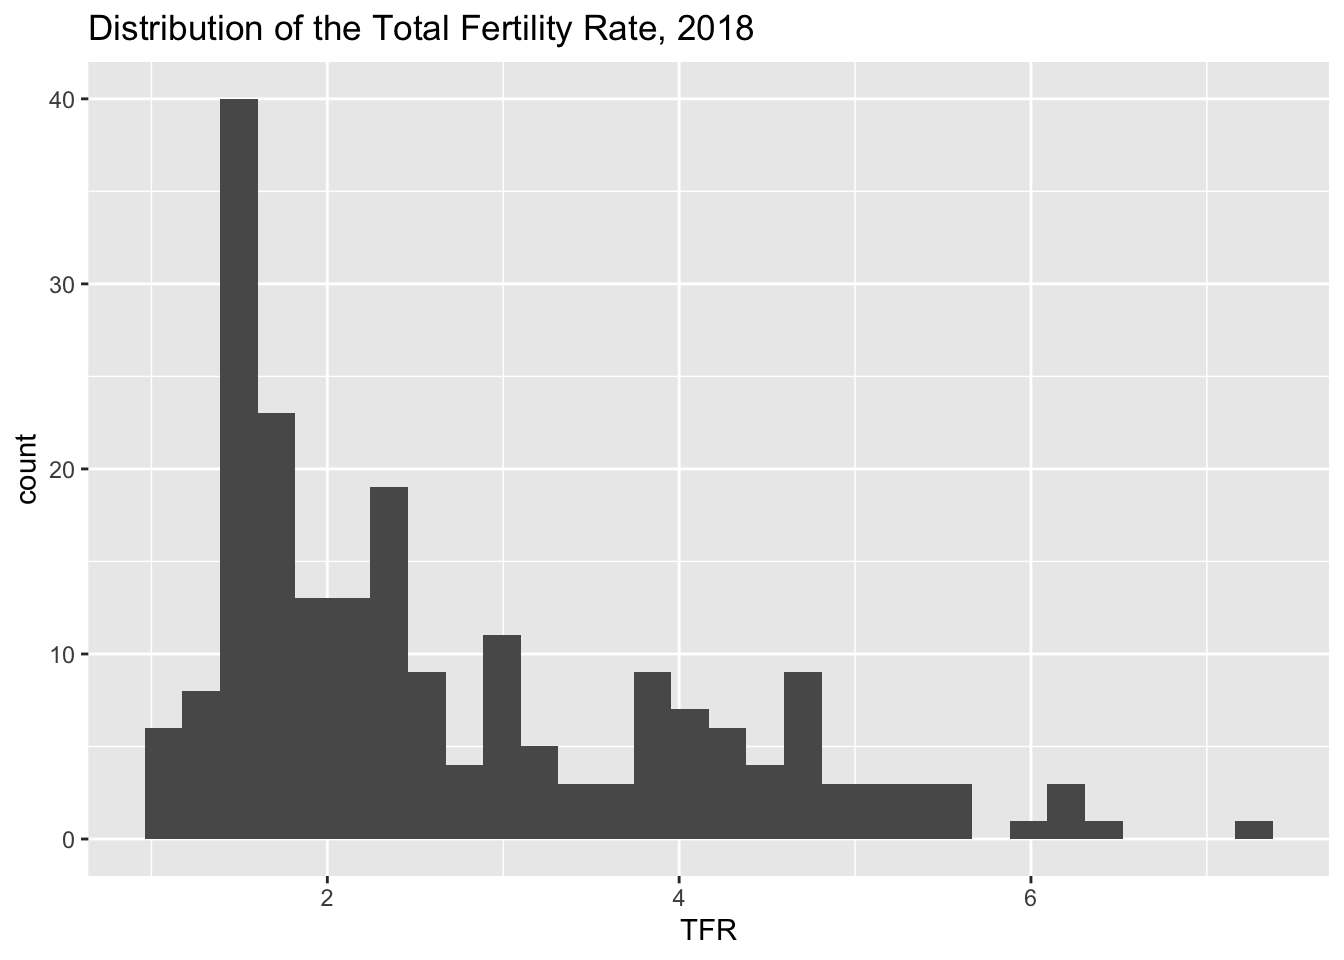
\includegraphics{rintro_files/figure-pdf/prbhist-1.pdf}

}

\end{figure}

The above example named the data frame explicitly in the
\texttt{ggplot()} call, but we can also use \texttt{dplyr} to pipe data
into the plot:

\begin{Shaded}
\begin{Highlighting}[]
\NormalTok{prb}\SpecialCharTok{\%\textgreater{}\%}
  \FunctionTok{ggplot}\NormalTok{(}\AttributeTok{mapping=}\FunctionTok{aes}\NormalTok{(}\AttributeTok{x =}\NormalTok{ tfr))}\SpecialCharTok{+}
  \FunctionTok{geom\_histogram}\NormalTok{()}\SpecialCharTok{+}
  \FunctionTok{ggtitle}\NormalTok{(}\AttributeTok{label =} \StringTok{"Distribution of the Total Fertility Rate, 2018"}\NormalTok{)}\SpecialCharTok{+}
  \FunctionTok{xlab}\NormalTok{(}\AttributeTok{label =} \StringTok{"TFR"}\NormalTok{)}
\end{Highlighting}
\end{Shaded}

\begin{verbatim}
`stat_bin()` using `bins = 30`. Pick better value with `binwidth`.
\end{verbatim}

\begin{figure}[H]

{\centering 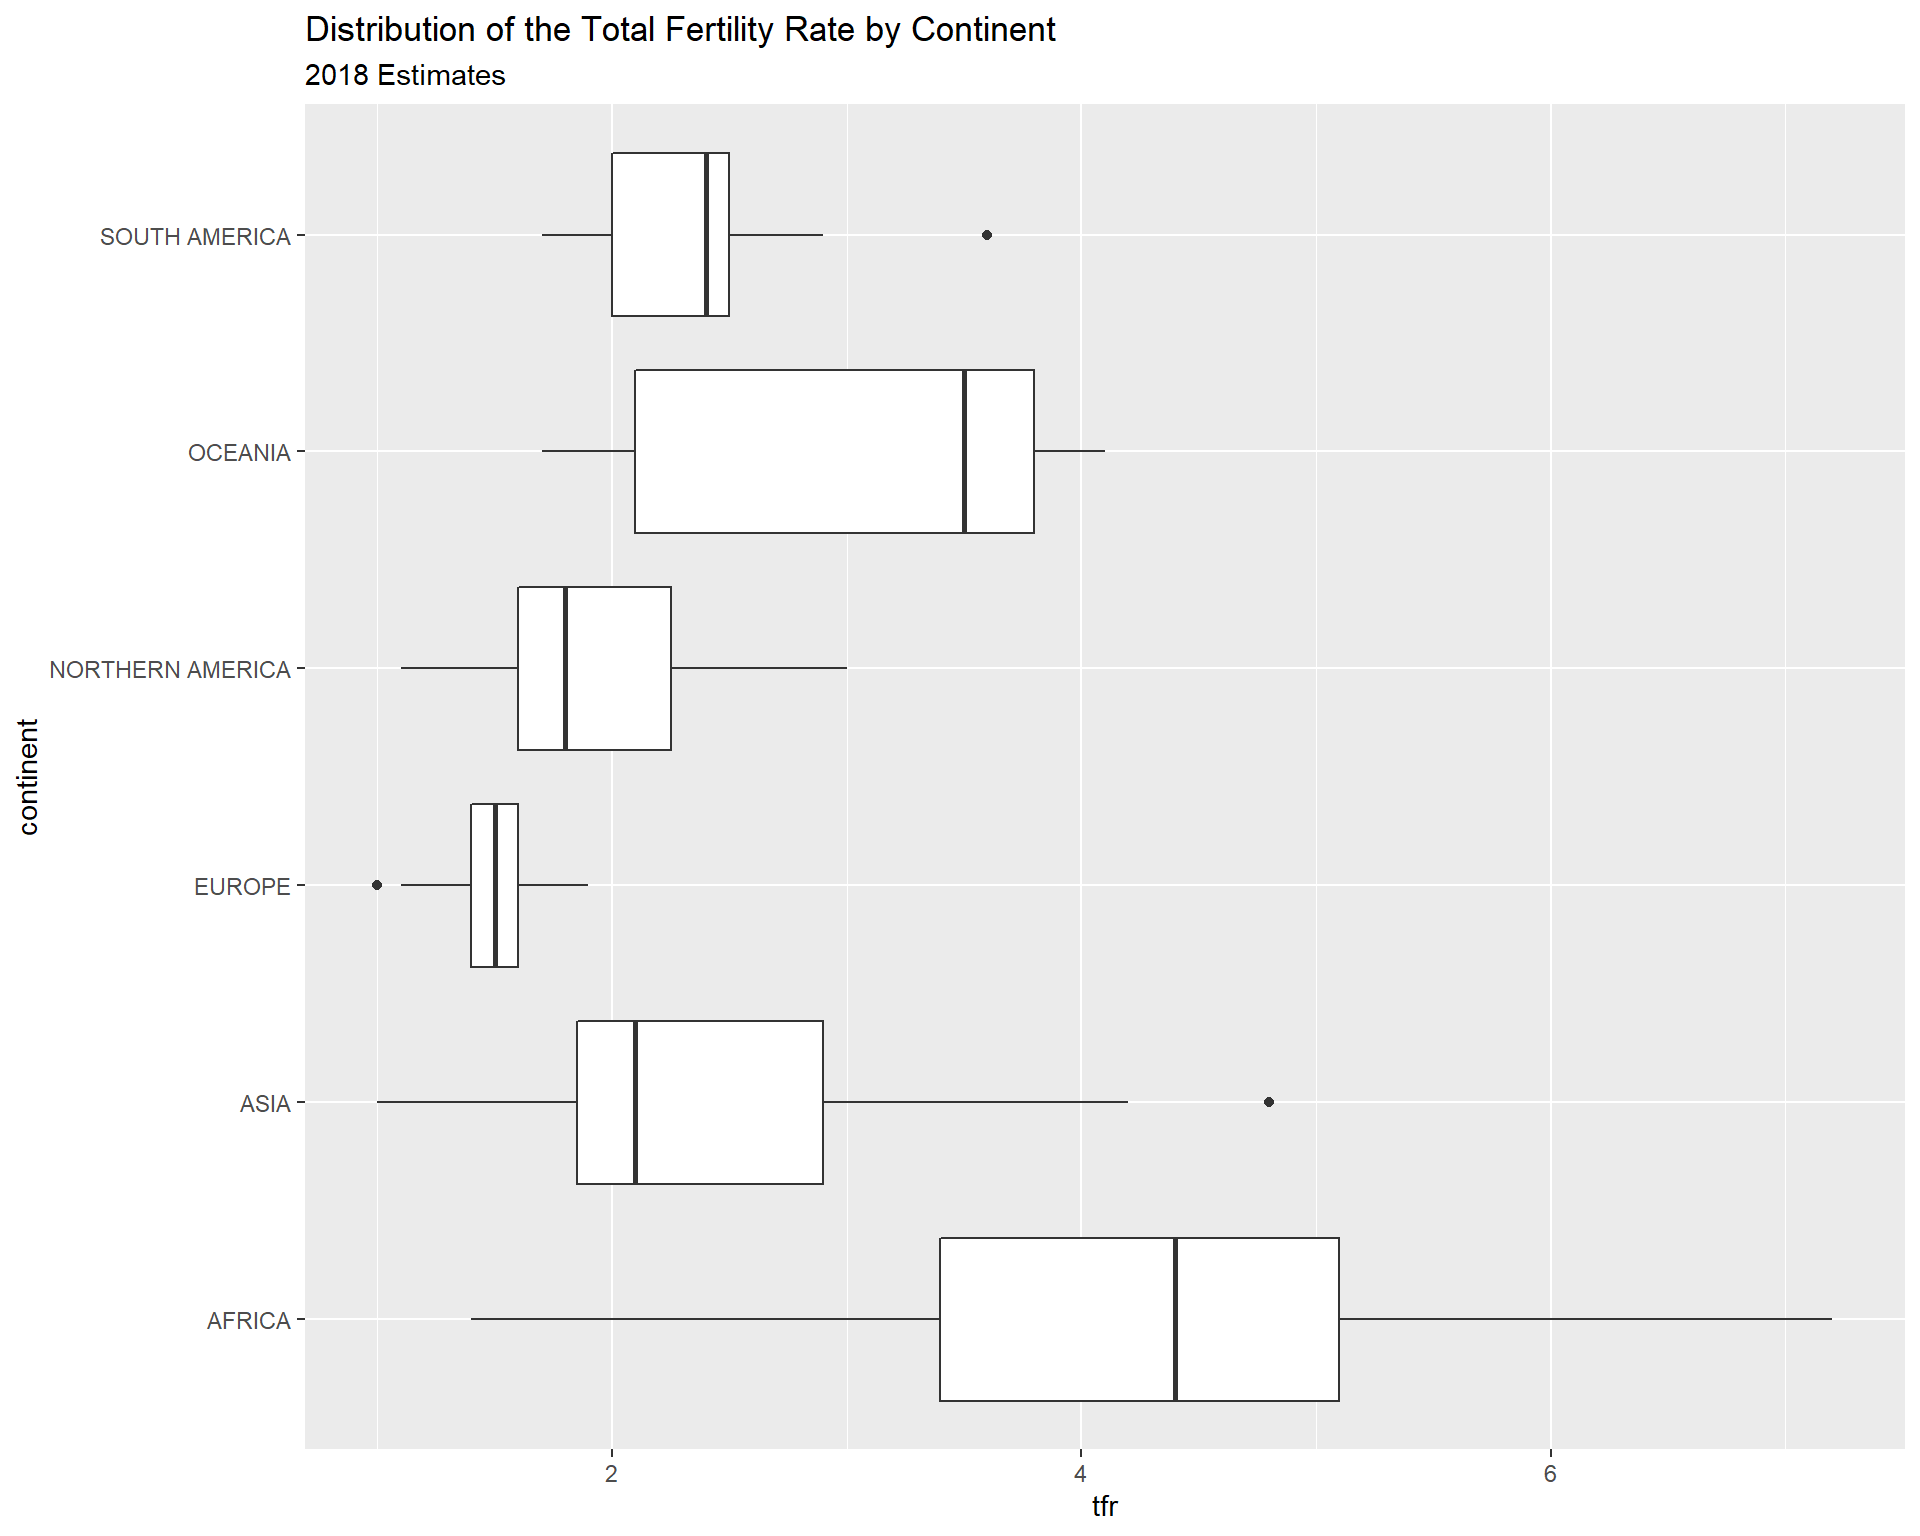
\includegraphics{rintro_files/figure-pdf/unnamed-chunk-68-1.pdf}

}

\end{figure}

We can likewise incorporate a \texttt{dplyr} workflow directly into our
plotting, using the example from before, we will create histograms for
the high and low fertility groups using the \texttt{facet\_wrap()}
function.

\begin{Shaded}
\begin{Highlighting}[]
\NormalTok{prb}\SpecialCharTok{\%\textgreater{}\%}
  \FunctionTok{mutate}\NormalTok{(}\AttributeTok{high\_tfr =} \FunctionTok{ifelse}\NormalTok{(}\AttributeTok{test =}\NormalTok{ tfr }\SpecialCharTok{\textgreater{}} \DecValTok{3}\NormalTok{,}
                           \AttributeTok{yes =} \StringTok{"high"}\NormalTok{,}
                           \AttributeTok{no =} \StringTok{"low"}\NormalTok{) )}\SpecialCharTok{\%\textgreater{}\%}
  \FunctionTok{group\_by}\NormalTok{(high\_tfr)}\SpecialCharTok{\%\textgreater{}\%}
  \FunctionTok{ggplot}\NormalTok{(}\AttributeTok{mapping=}\FunctionTok{aes}\NormalTok{(}\AttributeTok{x =}\NormalTok{ imr))}\SpecialCharTok{+}
  \FunctionTok{geom\_histogram}\NormalTok{(}\FunctionTok{aes}\NormalTok{( }\AttributeTok{fill =}\NormalTok{ high\_tfr))}\SpecialCharTok{+}
  \FunctionTok{facet\_wrap}\NormalTok{( }\SpecialCharTok{\textasciitilde{}}\NormalTok{ high\_tfr)}\SpecialCharTok{+}
  \FunctionTok{ggtitle}\NormalTok{(}\AttributeTok{label =} \StringTok{"Distribution of the Infant Mortality Rate, 2018"}\NormalTok{,}
          \AttributeTok{subtitle =} \StringTok{"Low and High Fertility Countries"}\NormalTok{)}\SpecialCharTok{+}
  \FunctionTok{xlab}\NormalTok{(}\AttributeTok{label =} \StringTok{"Infant Mortality Rate"}\NormalTok{)}
\end{Highlighting}
\end{Shaded}

\begin{verbatim}
`stat_bin()` using `bins = 30`. Pick better value with `binwidth`.
\end{verbatim}

\begin{verbatim}
Warning: Removed 1 rows containing non-finite values (`stat_bin()`).
\end{verbatim}

\begin{figure}[H]

{\centering 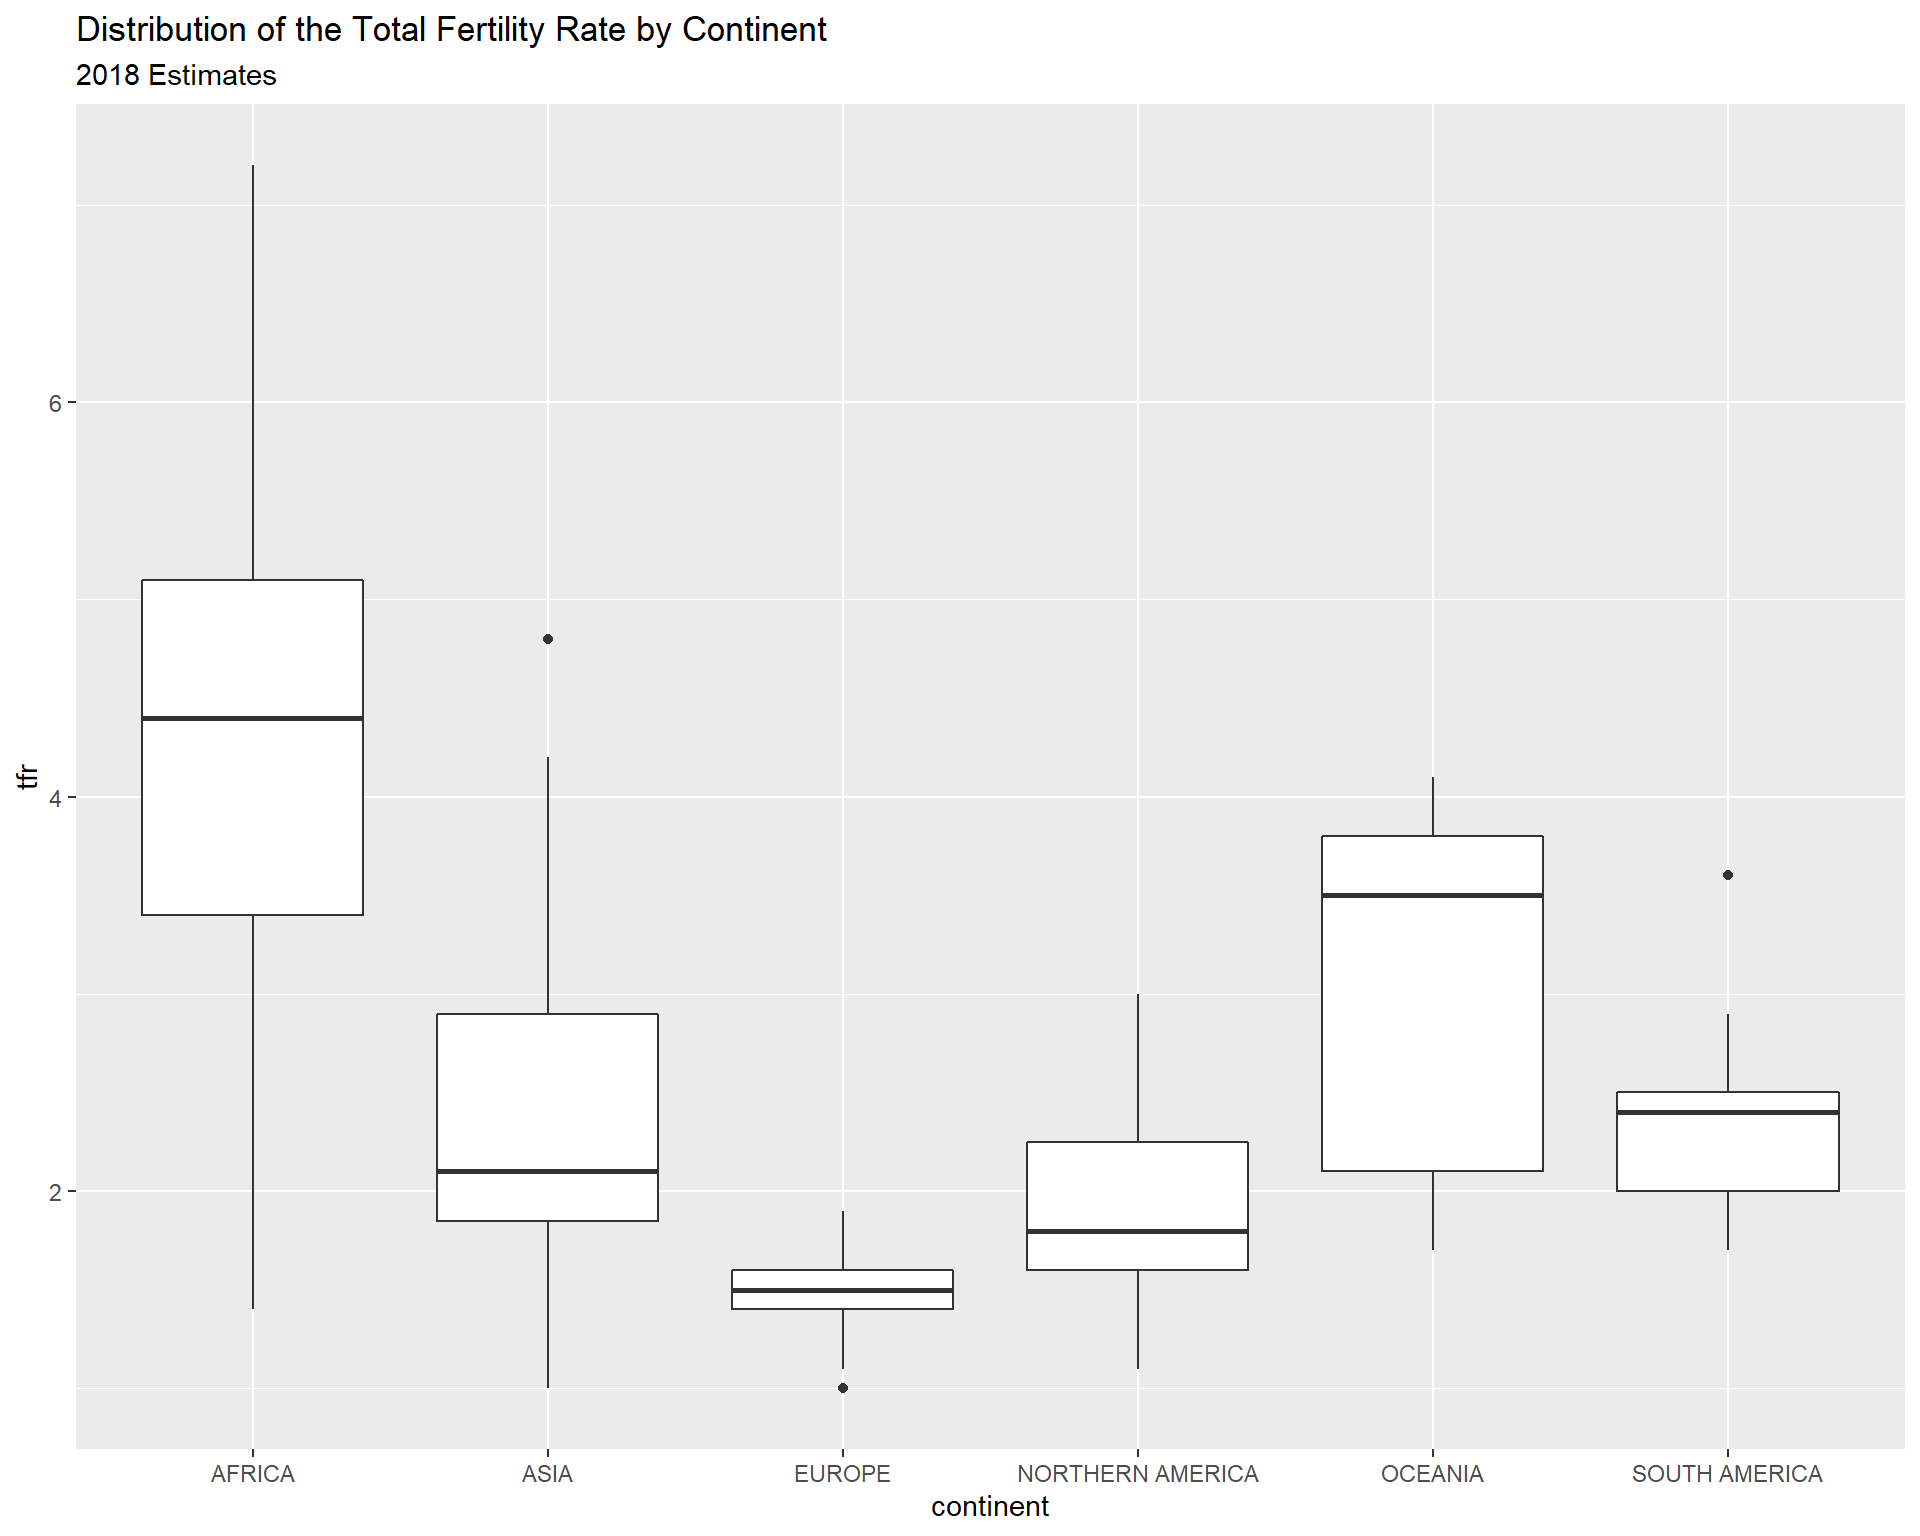
\includegraphics{rintro_files/figure-pdf/unnamed-chunk-69-1.pdf}

}

\end{figure}

You also notice that I used the \texttt{aes(fill\ =\ high\_tfr)} to tell
R to color the histogram bars according to the variable
\texttt{high\_tfr}. The \texttt{aes()} function allows you to modify
colors, line types, and fills based of values of a variable.

Another way to display the distribution of a variable is to use
\texttt{geom\_density()} which calculates the kernel density of a
variable. Again, I use a variable, this time the continent a country is
on, to color the lines for the plot.

\begin{Shaded}
\begin{Highlighting}[]
\NormalTok{prb}\SpecialCharTok{\%\textgreater{}\%}
\FunctionTok{ggplot}\NormalTok{(}\AttributeTok{mapping =} \FunctionTok{aes}\NormalTok{(tfr,}
                     \AttributeTok{colour =}\NormalTok{ continent,}
                     \AttributeTok{stat =}\NormalTok{ ..density..))}\SpecialCharTok{+}
  \FunctionTok{geom\_density}\NormalTok{()}\SpecialCharTok{+}
  \FunctionTok{ggtitle}\NormalTok{(}\AttributeTok{label =} \StringTok{"Distribution of the Total Fertility Rate by Continent"}\NormalTok{,}
          \AttributeTok{subtitle =} \StringTok{"2018 Estimates"}\NormalTok{)}\SpecialCharTok{+}
  \FunctionTok{xlab}\NormalTok{(}\AttributeTok{label =} \StringTok{"TFR"}\NormalTok{)}
\end{Highlighting}
\end{Shaded}

\begin{verbatim}
Warning: The dot-dot notation (`..density..`) was deprecated in ggplot2 3.4.0.
i Please use `after_stat(density)` instead.
\end{verbatim}

\begin{figure}[H]

{\centering 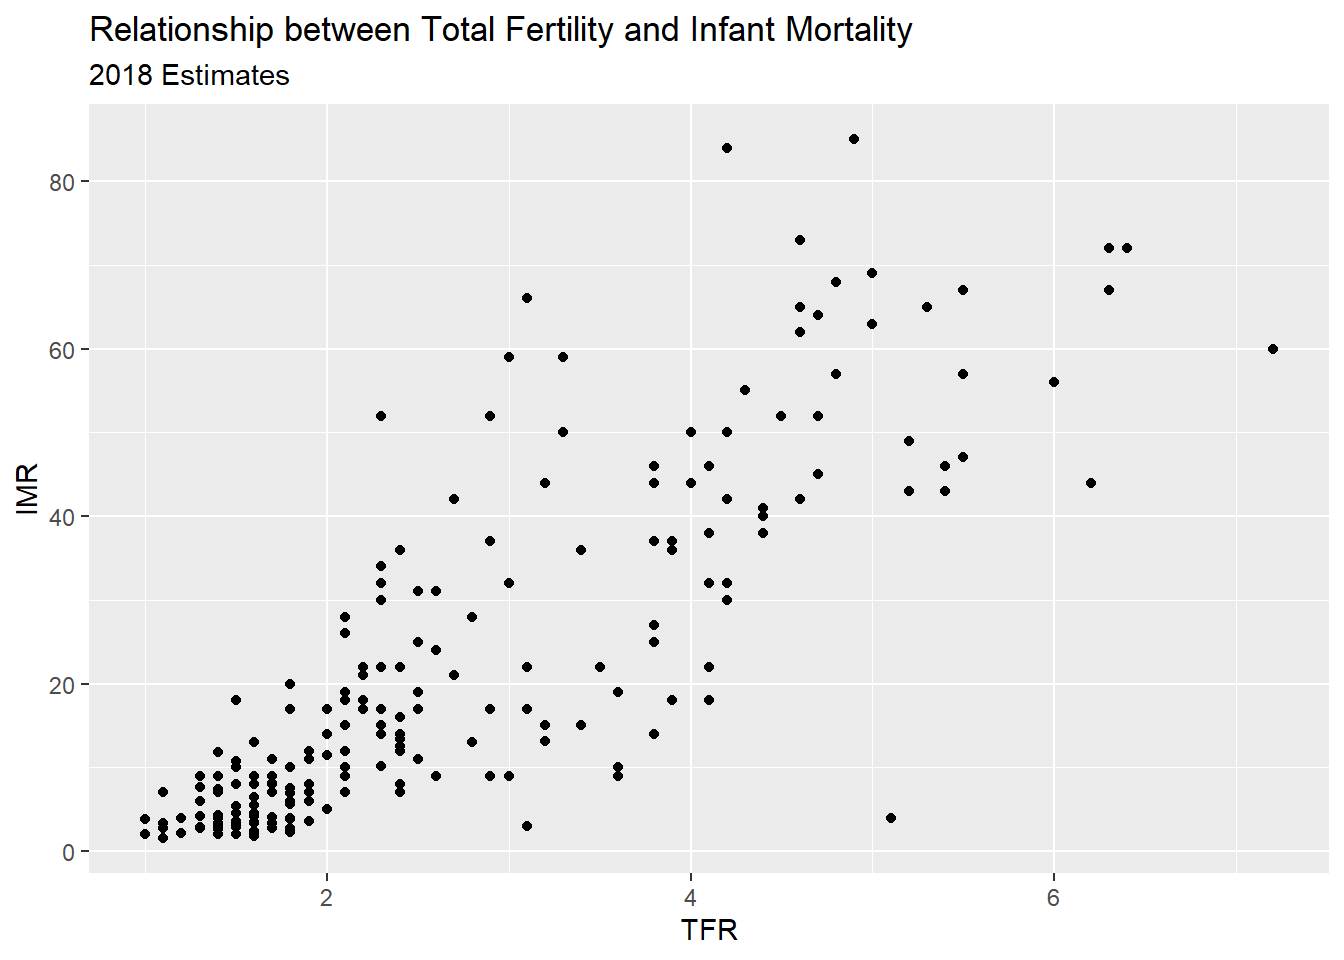
\includegraphics{rintro_files/figure-pdf/unnamed-chunk-70-1.pdf}

}

\end{figure}

\hypertarget{stem-and-leaf-plotsbox-and-whisker-plots}{%
\subsection{Stem and leaf plots/Box and Whisker
plots}\label{stem-and-leaf-plotsbox-and-whisker-plots}}

Another visualization method is the stem and leaf plot, or box and
whisker plot. This is useful when you have a continuous variable you
want to display the distribution of across levels of a categorical
variable. This is basically a graphical display of Tukey's 5 number
summary of data.

\begin{Shaded}
\begin{Highlighting}[]
\NormalTok{prb}\SpecialCharTok{\%\textgreater{}\%}
  \FunctionTok{ggplot}\NormalTok{( }\AttributeTok{mapping =} \FunctionTok{aes}\NormalTok{(}\AttributeTok{x =}\NormalTok{ continent, }\AttributeTok{y =}\NormalTok{ tfr))}\SpecialCharTok{+}
  \FunctionTok{geom\_boxplot}\NormalTok{()}\SpecialCharTok{+}
  \FunctionTok{ggtitle}\NormalTok{(}\AttributeTok{label =} \StringTok{"Distribution of the Total Fertility Rate by Continent"}\NormalTok{,}
          \AttributeTok{subtitle =} \StringTok{"2018 Estimates"}\NormalTok{)}
\end{Highlighting}
\end{Shaded}

\begin{figure}[H]

{\centering 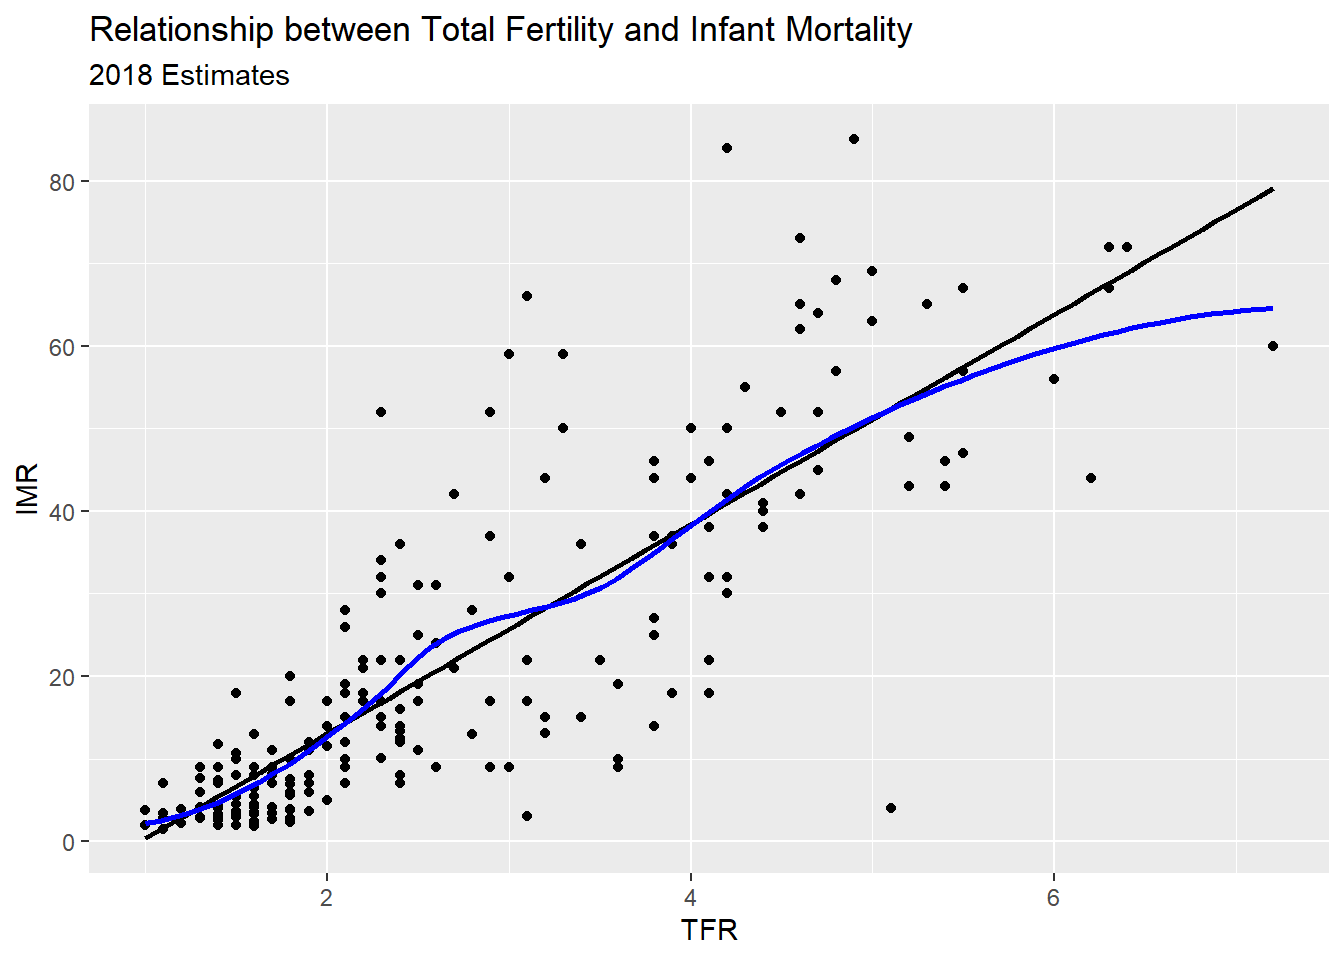
\includegraphics{rintro_files/figure-pdf/unnamed-chunk-71-1.pdf}

}

\end{figure}

You can flip the axes, by adding \texttt{coord\_flip()}

\begin{Shaded}
\begin{Highlighting}[]
\NormalTok{prb}\SpecialCharTok{\%\textgreater{}\%}
\FunctionTok{ggplot}\NormalTok{( }\AttributeTok{mapping =} \FunctionTok{aes}\NormalTok{( }\AttributeTok{x =}\NormalTok{ continent,}
                       \AttributeTok{y =}\NormalTok{ tfr))}\SpecialCharTok{+}
  \FunctionTok{geom\_boxplot}\NormalTok{()}\SpecialCharTok{+}
  \FunctionTok{ggtitle}\NormalTok{(}\AttributeTok{label =} \StringTok{"Distribution of the Total Fertility Rate by Continent"}\NormalTok{,}
          \AttributeTok{subtitle =} \StringTok{"2018 Estimates"}\NormalTok{)}\SpecialCharTok{+}
  \FunctionTok{coord\_flip}\NormalTok{()}
\end{Highlighting}
\end{Shaded}

\begin{figure}[H]

{\centering 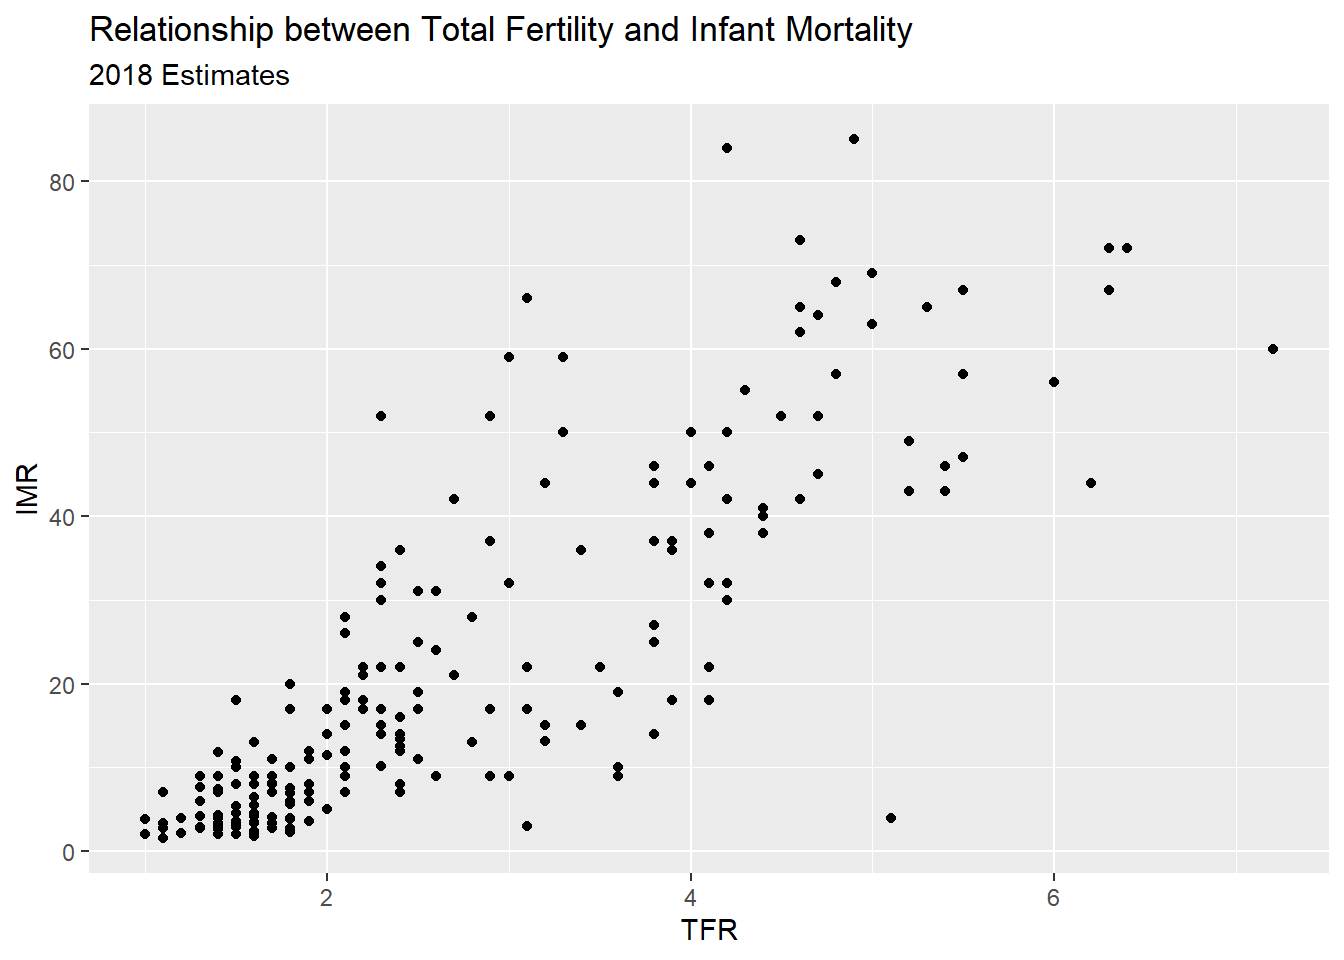
\includegraphics{rintro_files/figure-pdf/unnamed-chunk-72-1.pdf}

}

\end{figure}

You can also color the boxes by a variable, Here, I will make a new
variable that is the combination of the continent variable with the
region variable, using the \texttt{paste()} function. It's useful for
combining values of two strings.

\begin{Shaded}
\begin{Highlighting}[]
\NormalTok{prb}\SpecialCharTok{\%\textgreater{}\%}
  \FunctionTok{mutate}\NormalTok{(}\AttributeTok{newname =} \FunctionTok{paste}\NormalTok{(continent, region, }\AttributeTok{sep =} \StringTok{"{-}"}\NormalTok{))}\SpecialCharTok{\%\textgreater{}\%}
  \FunctionTok{ggplot}\NormalTok{(}\FunctionTok{aes}\NormalTok{(}\AttributeTok{x =}\NormalTok{ newname,}
             \AttributeTok{y =}\NormalTok{ tfr,}
             \AttributeTok{fill =}\NormalTok{ continent))}\SpecialCharTok{+}
  \FunctionTok{geom\_boxplot}\NormalTok{()}\SpecialCharTok{+}
  \FunctionTok{coord\_flip}\NormalTok{()}\SpecialCharTok{+}
  \FunctionTok{ggtitle}\NormalTok{(}\AttributeTok{label =} \StringTok{"Distribution of the Total Fertility Rate by Continent"}\NormalTok{,}
          \AttributeTok{subtitle =} \StringTok{"2018 Estimates"}\NormalTok{)}
\end{Highlighting}
\end{Shaded}

\begin{figure}[H]

{\centering 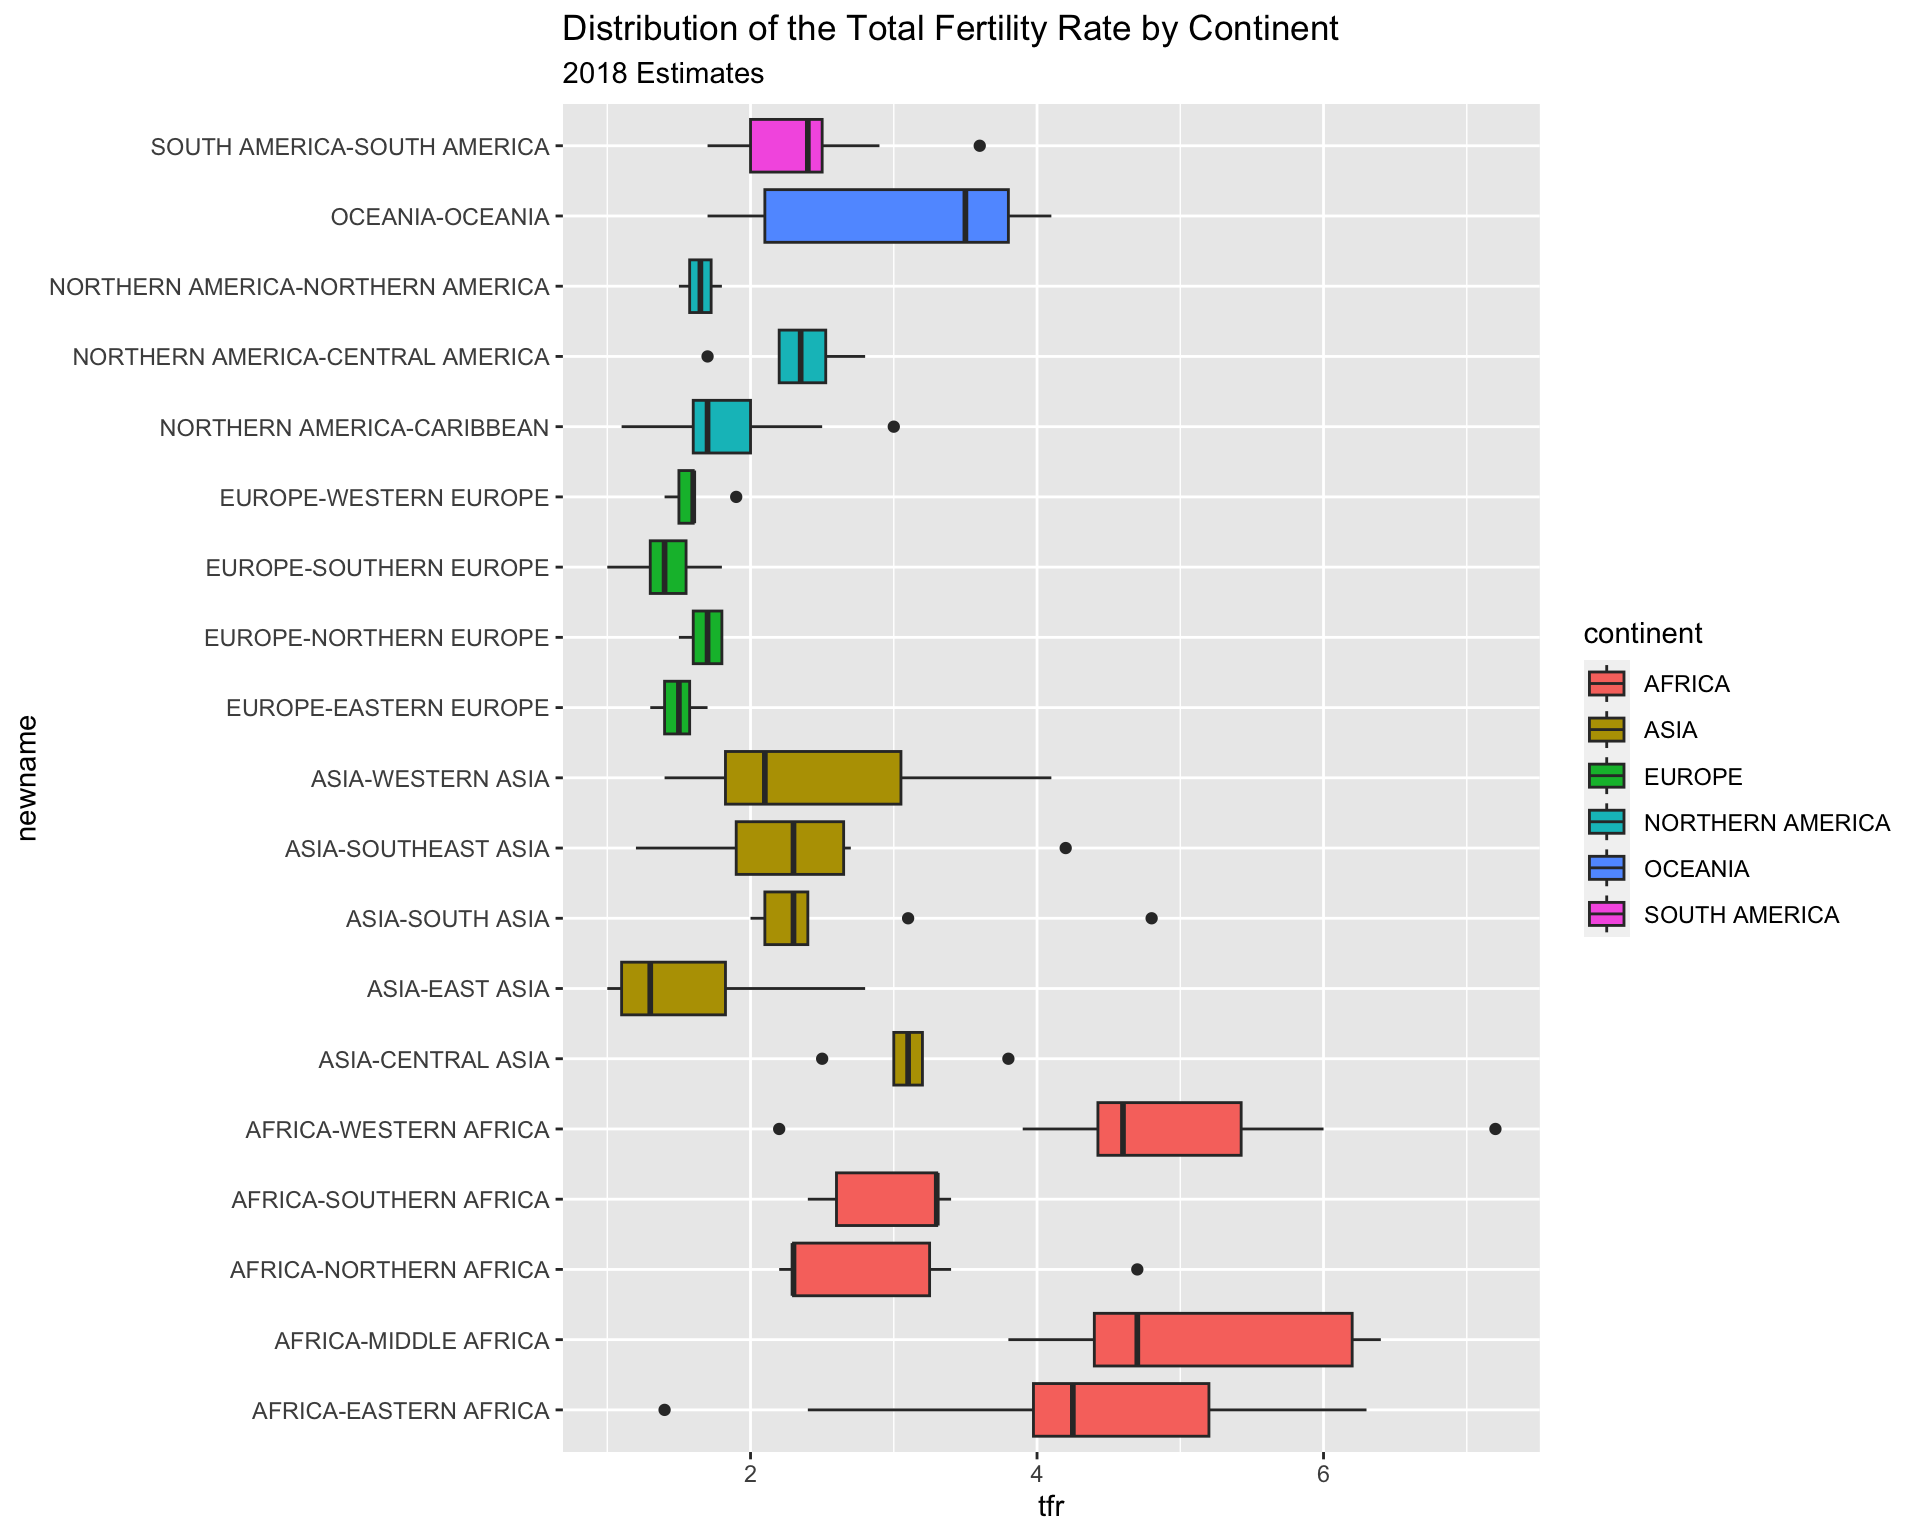
\includegraphics{rintro_files/figure-pdf/unnamed-chunk-73-1.pdf}

}

\end{figure}

\hypertarget{x-y-scatter-plots}{%
\subsection{X-Y Scatter plots}\label{x-y-scatter-plots}}

These are useful for finding relationships among two or more continuous
variables. \texttt{ggplot()} can really make these pretty. The
\texttt{geom\_point()} geometry adds points to the plot.

Here are a few riffs using the PRB data:

\begin{Shaded}
\begin{Highlighting}[]
\NormalTok{prb}\SpecialCharTok{\%\textgreater{}\%}
\FunctionTok{ggplot}\NormalTok{(}\AttributeTok{mapping=} \FunctionTok{aes}\NormalTok{(}\AttributeTok{x =}\NormalTok{ tfr,}
                    \AttributeTok{y =}\NormalTok{ imr))}\SpecialCharTok{+}
  \FunctionTok{geom\_point}\NormalTok{()}\SpecialCharTok{+}
  \FunctionTok{ggtitle}\NormalTok{(}\AttributeTok{label =} \StringTok{"Relationship between Total Fertility and Infant Mortality"}\NormalTok{,}
          \AttributeTok{subtitle =} \StringTok{"2018 Estimates"}\NormalTok{)}\SpecialCharTok{+}
  \FunctionTok{xlab}\NormalTok{(}\AttributeTok{label =} \StringTok{"TFR"}\NormalTok{)}\SpecialCharTok{+}
  \FunctionTok{ylab}\NormalTok{(}\AttributeTok{label =} \StringTok{"IMR"}\NormalTok{)}
\end{Highlighting}
\end{Shaded}

\begin{verbatim}
Warning: Removed 1 rows containing missing values (`geom_point()`).
\end{verbatim}

\begin{figure}[H]

{\centering 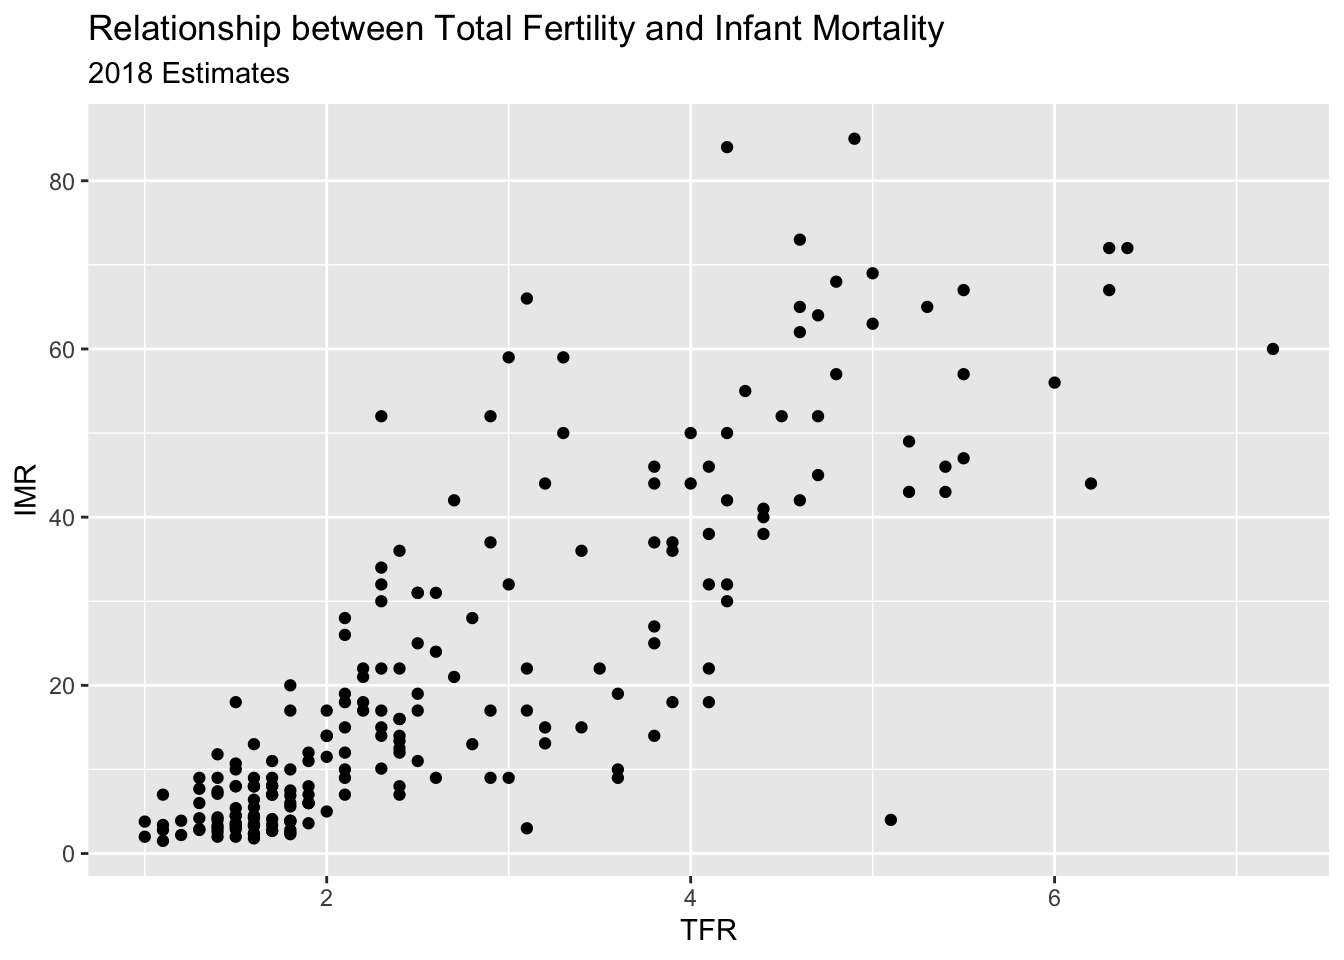
\includegraphics{rintro_files/figure-pdf/unnamed-chunk-74-1.pdf}

}

\end{figure}

R also makes it easy to overlay linear and spline smoothers for the data
(more on splines later).

\begin{Shaded}
\begin{Highlighting}[]
\NormalTok{prb}\SpecialCharTok{\%\textgreater{}\%}
\FunctionTok{ggplot}\NormalTok{(}\AttributeTok{mapping =} \FunctionTok{aes}\NormalTok{(}\AttributeTok{x =}\NormalTok{ tfr,}
                    \AttributeTok{y =}\NormalTok{ imr))}\SpecialCharTok{+}
  \FunctionTok{geom\_point}\NormalTok{()}\SpecialCharTok{+}
  \FunctionTok{geom\_smooth}\NormalTok{(}\AttributeTok{method =} \StringTok{"lm"}\NormalTok{,}
              \AttributeTok{color =} \StringTok{"black"}\NormalTok{,}
              \AttributeTok{se =}\NormalTok{ F)}\SpecialCharTok{+} \CommentTok{\#linear regression fit}
  \FunctionTok{geom\_smooth}\NormalTok{(}\AttributeTok{color =} \StringTok{"blue"}\NormalTok{,}
              \AttributeTok{method =} \StringTok{"loess"}\NormalTok{,}
              \AttributeTok{se =} \ConstantTok{FALSE}\NormalTok{)}\SpecialCharTok{+}
  \FunctionTok{ggtitle}\NormalTok{(}\AttributeTok{label =} \StringTok{"Relationship between Total Fertility and Infant Mortality"}\NormalTok{,}
          \AttributeTok{subtitle =} \StringTok{"2018 Estimates"}\NormalTok{)}\SpecialCharTok{+}
  \FunctionTok{xlab}\NormalTok{(}\AttributeTok{label =} \StringTok{"TFR"}\NormalTok{)}\SpecialCharTok{+}
  \FunctionTok{ylab}\NormalTok{(}\AttributeTok{label =} \StringTok{"IMR"}\NormalTok{)}
\end{Highlighting}
\end{Shaded}

\begin{figure}[H]

{\centering 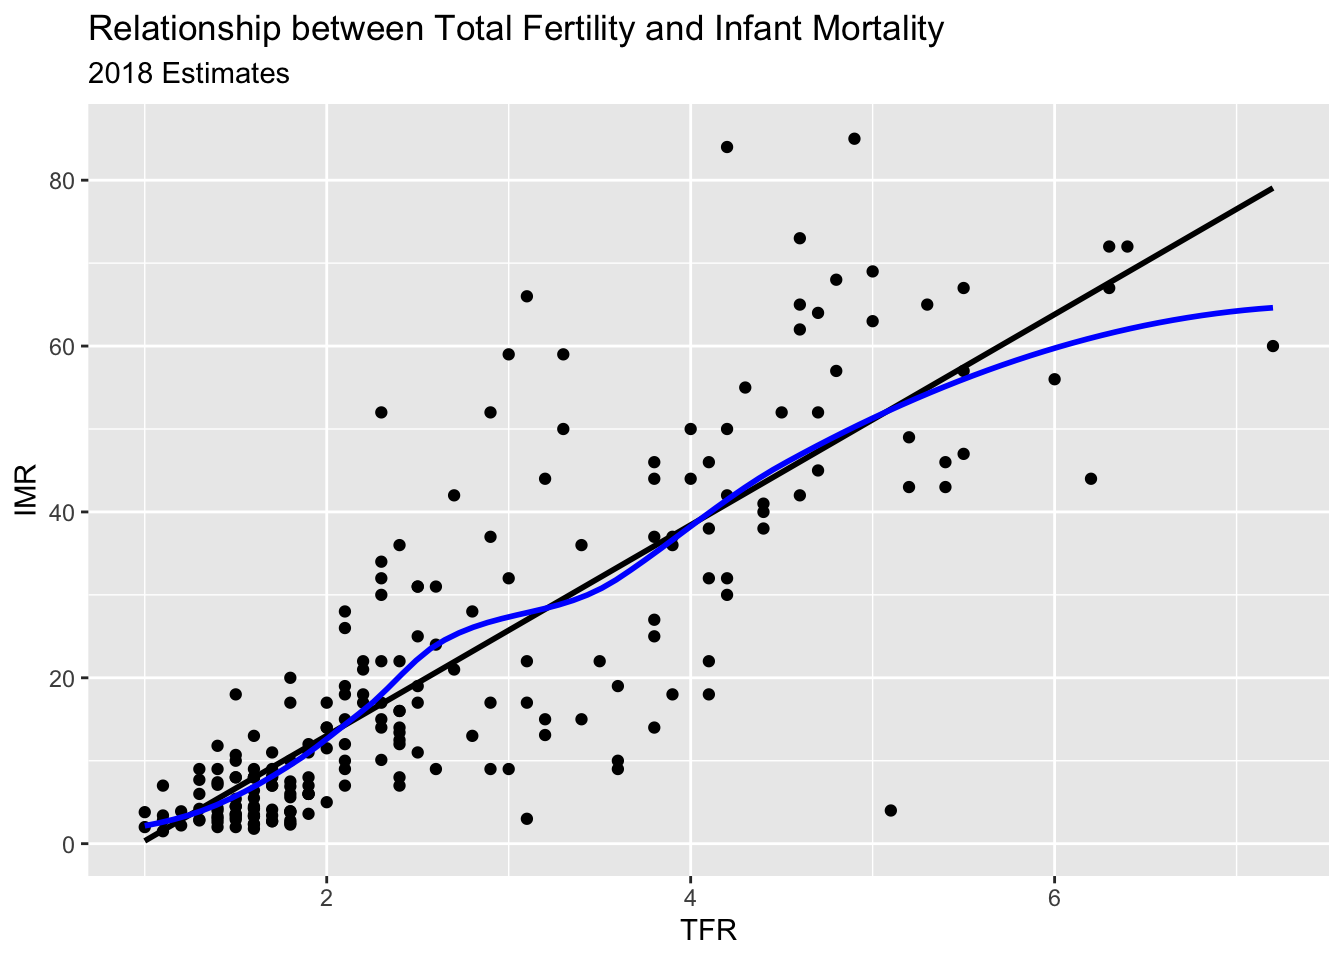
\includegraphics{rintro_files/figure-pdf/unnamed-chunk-75-1.pdf}

}

\end{figure}

Now we color the points by continent

\begin{Shaded}
\begin{Highlighting}[]
\NormalTok{prb}\SpecialCharTok{\%\textgreater{}\%}
\FunctionTok{ggplot}\NormalTok{(}\AttributeTok{mapping =} \FunctionTok{aes}\NormalTok{(}\AttributeTok{x =}\NormalTok{ tfr, }
                     \AttributeTok{y =}\NormalTok{ imr,}
                     \AttributeTok{color =}\NormalTok{continent))}\SpecialCharTok{+}
  \FunctionTok{geom\_point}\NormalTok{()}\SpecialCharTok{+}
  \FunctionTok{geom\_smooth}\NormalTok{(}\AttributeTok{method =} \StringTok{"lm"}\NormalTok{,}
              \AttributeTok{se =} \ConstantTok{FALSE}\NormalTok{)}\SpecialCharTok{+}
  \FunctionTok{ggtitle}\NormalTok{(}\AttributeTok{label =} \StringTok{"Relationship between Total Fertility and Infant Mortality"}\NormalTok{,}
          \AttributeTok{subtitle =} \StringTok{"2018 Estimates"}\NormalTok{)}\SpecialCharTok{+}
  \FunctionTok{xlab}\NormalTok{(}\AttributeTok{label =} \StringTok{"TFR"}\NormalTok{)}\SpecialCharTok{+}
  \FunctionTok{ylab}\NormalTok{(}\AttributeTok{label =} \StringTok{"IMR"}\NormalTok{)}
\end{Highlighting}
\end{Shaded}

\begin{figure}[H]

{\centering 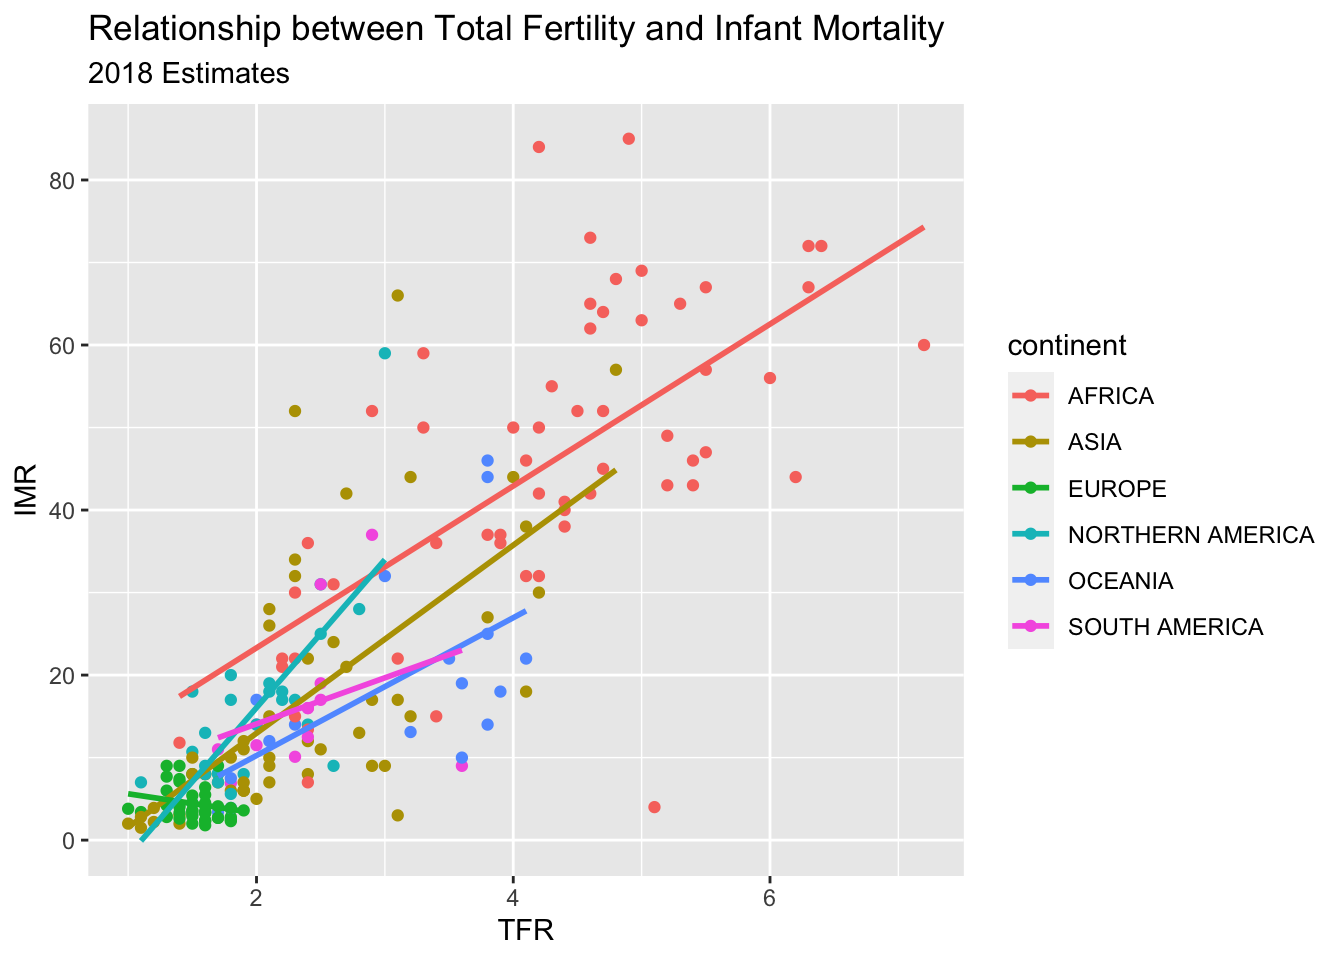
\includegraphics{rintro_files/figure-pdf/unnamed-chunk-76-1.pdf}

}

\end{figure}

\hypertarget{facet-plots}{%
\subsection{Facet plots}\label{facet-plots}}

Facet plots are nice, they allow you to create a plot separately based
on a grouping variable. This allows you to visualize if the relationship
is constant across those groups. Here, I repeat the plot above, but I
facet on the continent, and include the regression line for each
continent.

\begin{Shaded}
\begin{Highlighting}[]
\NormalTok{prb}\SpecialCharTok{\%\textgreater{}\%}
\FunctionTok{ggplot}\NormalTok{(}\AttributeTok{mapping=} \FunctionTok{aes}\NormalTok{(}\AttributeTok{x =}\NormalTok{ tfr,}
                    \AttributeTok{y =}\NormalTok{ imr,}
                    \AttributeTok{color =}\NormalTok{ continent))}\SpecialCharTok{+}
  \FunctionTok{geom\_point}\NormalTok{()}\SpecialCharTok{+}
  \FunctionTok{geom\_smooth}\NormalTok{(}\AttributeTok{method =} \StringTok{"lm"}\NormalTok{,}
              \AttributeTok{se =} \ConstantTok{FALSE}\NormalTok{,}
              \AttributeTok{color =} \StringTok{"black"}\NormalTok{)}\SpecialCharTok{+}
  \FunctionTok{facet\_wrap}\NormalTok{( }\SpecialCharTok{\textasciitilde{}}\NormalTok{ continent)}\SpecialCharTok{+}
  \FunctionTok{ggtitle}\NormalTok{(}\AttributeTok{label =} \StringTok{"Relationship between Total Fertility and Infant Mortality"}\NormalTok{,}
          \AttributeTok{subtitle =} \StringTok{"2018 Estimates"}\NormalTok{)}\SpecialCharTok{+}
  \FunctionTok{xlab}\NormalTok{(}\AttributeTok{label =} \StringTok{"TFR"}\NormalTok{)}\SpecialCharTok{+}
  \FunctionTok{ylab}\NormalTok{(}\AttributeTok{label =} \StringTok{"IMR"}\NormalTok{)}
\end{Highlighting}
\end{Shaded}

\begin{figure}[H]

{\centering 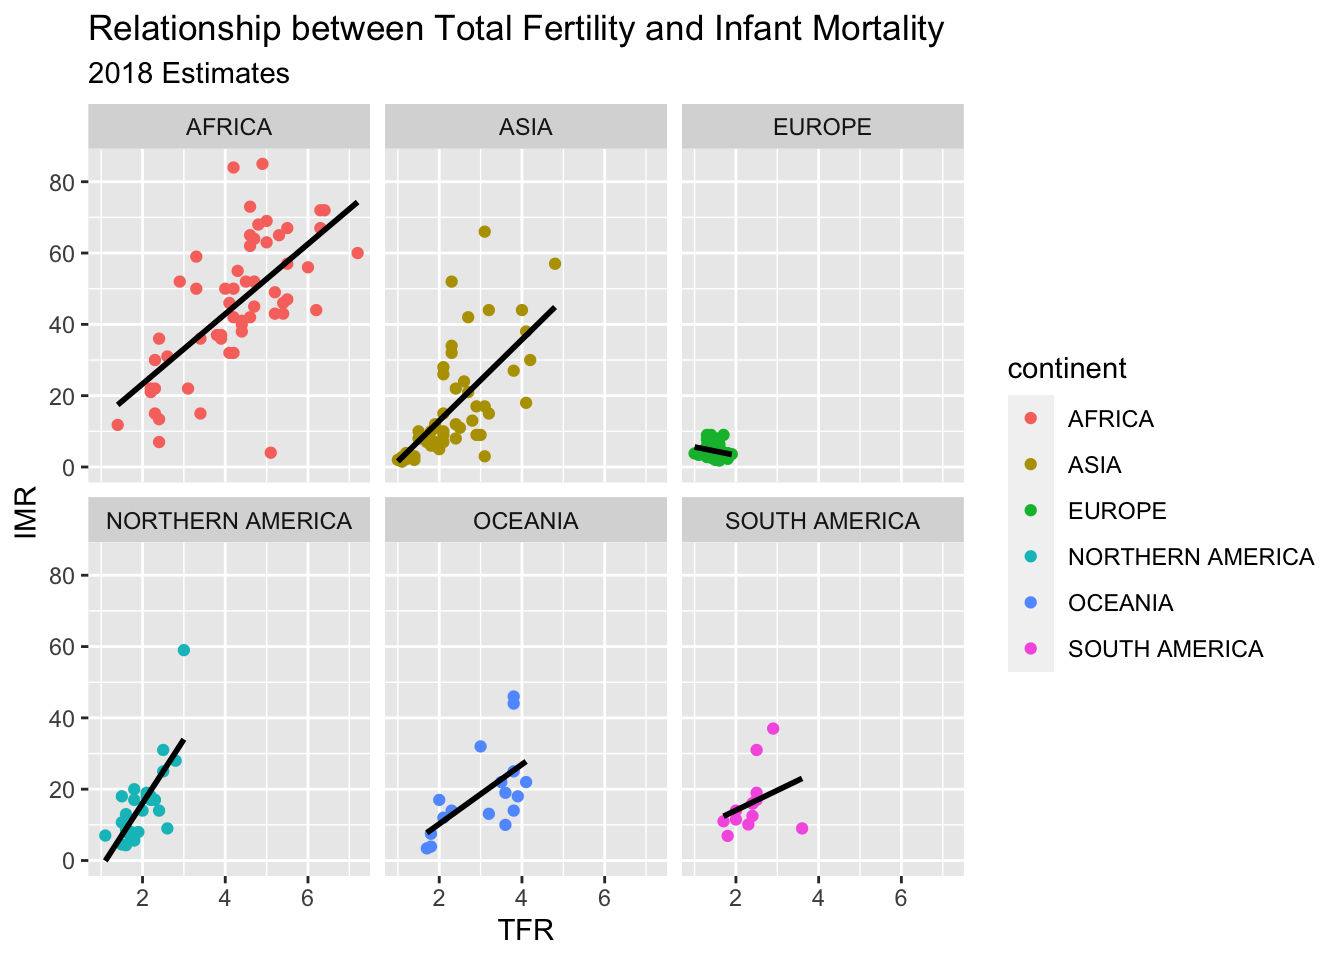
\includegraphics{rintro_files/figure-pdf/unnamed-chunk-77-1.pdf}

}

\end{figure}

Another example, this time of a bad linear plot! \texttt{ggplot} makes
it easy to examine if a relationship is linear or curvilinear, at least
visually.

\begin{Shaded}
\begin{Highlighting}[]
\FunctionTok{ggplot}\NormalTok{(}\AttributeTok{data =}\NormalTok{ prb,}\AttributeTok{mapping =} \FunctionTok{aes}\NormalTok{(}\AttributeTok{x =}\NormalTok{ tfr, }\AttributeTok{y =}\NormalTok{ pctlt15\_2018))}\SpecialCharTok{+}
  \FunctionTok{geom\_point}\NormalTok{()}\SpecialCharTok{+}
  \FunctionTok{geom\_smooth}\NormalTok{( }\AttributeTok{method =} \StringTok{"lm"}\NormalTok{,}
               \AttributeTok{se =} \ConstantTok{FALSE}\NormalTok{,}
               \AttributeTok{color =} \StringTok{"black"}\NormalTok{)}\SpecialCharTok{+}
  \FunctionTok{geom\_smooth}\NormalTok{( }\AttributeTok{method =} \StringTok{"loess"}\NormalTok{,}
               \AttributeTok{se =} \ConstantTok{FALSE}\NormalTok{,}
               \AttributeTok{color =} \StringTok{"blue"}\NormalTok{)}\SpecialCharTok{+}
  \FunctionTok{ggtitle}\NormalTok{(}\AttributeTok{label =} \StringTok{"Relationship between Total Fertility and Percent under age 15"}\NormalTok{,}
          \AttributeTok{subtitle =} \StringTok{"2018 Estimates{-} Linear \& Loess fit"}\NormalTok{)}\SpecialCharTok{+}
  \FunctionTok{xlab}\NormalTok{(}\AttributeTok{label =} \StringTok{"Percent under age 15"}\NormalTok{)}\SpecialCharTok{+}
  \FunctionTok{ylab}\NormalTok{(}\AttributeTok{label =} \StringTok{"IMR"}\NormalTok{)}
\end{Highlighting}
\end{Shaded}

\begin{verbatim}
`geom_smooth()` using formula = 'y ~ x'
`geom_smooth()` using formula = 'y ~ x'
\end{verbatim}

\begin{figure}[H]

{\centering 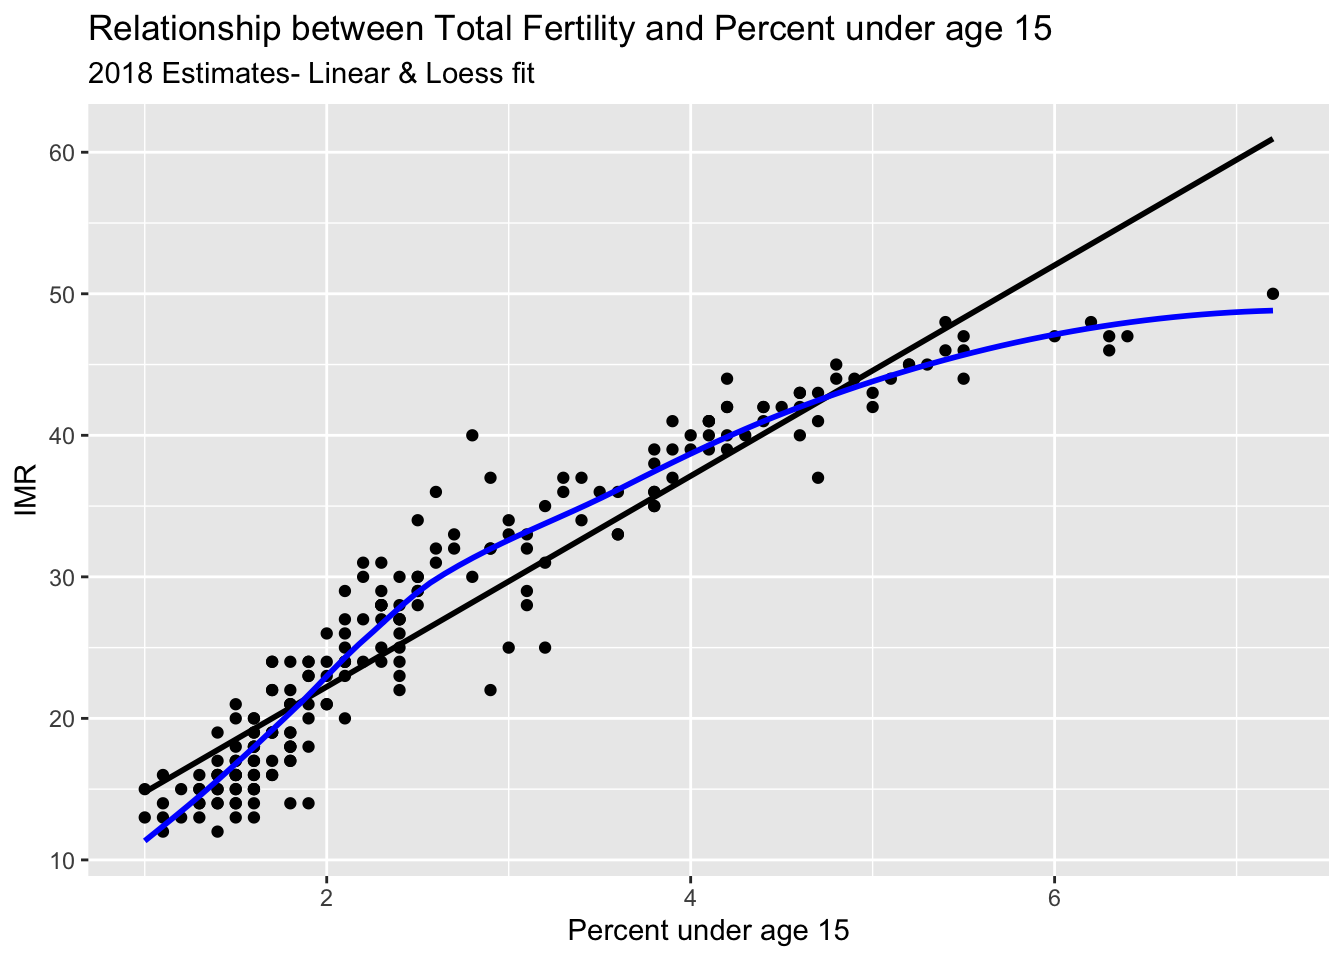
\includegraphics{rintro_files/figure-pdf/unnamed-chunk-78-1.pdf}

}

\end{figure}

\hypertarget{chapter-summary}{%
\section{Chapter summary}\label{chapter-summary}}

In this chapter, I have introduced R and Rstudio and some basic uses of
the software for accessing data and estimating some summary statistics.
The R ecosystem is large and complex, and the goal of this book is to
show you, the user, how to use R for analyzing data from demographic
data sources. In the chapters that follow, I will show how to use R
within two large universes of data, the macro and the micro. The
\emph{macro} level sections will focus on using R on data that come
primarily from places - nations, regions, administrative areas. The
\emph{micro} level sections will focus on analyzing complex survey data
on individual responses to demographic surveys. The final section will
discuss approaches that merge these two levels into a multi-level
framework and describe how such models are estimated and applied.

\hypertarget{references}{%
\section{References}\label{references}}

\bookmarksetup{startatroot}

\hypertarget{analysis-of-survey-data}{%
\chapter{Analysis of Survey Data}\label{analysis-of-survey-data}}

\newpage

\bookmarksetup{startatroot}

\hypertarget{survey-data}{%
\chapter{Survey Data}\label{survey-data}}

\hypertarget{demographic-survey-data}{%
\section{Demographic Survey data}\label{demographic-survey-data}}

The majority of demographic research relies on two or three main sources
of information. First among these are population enumerations or
censuses, followed by vital registration data on births and deaths and
last but not least, data from surveys. Censuses and other population
enumerations are typically undertaken by federal statistical agencies
and demographers use this data once it's disseminated from these
agencies. Similarly, vital registration data are usually collected by
governmental agencies, who oversee the collection and data quality for
the data. Survey data on the other hand can come from a wide variety of
sources.

It's not uncommon for us to go and collect our own survey data specific
to a research project we have, typically on a specialized population
that we are interested in learning about, but surveys can also be quite
general in their scope and collect information on a wide variety of
subjects. Owing to the mix of small and large-scale survey data
collection efforts, survey data are often available on many different
topics, locales and time periods. Of course we as demographers are
typically interested in population-level analysis or generalization from
our work, so the survey data we try to use are collected in rigorous
manners, with much attention and forethought paid to ensure the data we
collect can actually be representative of the \emph{target population}
we are trying to describe.

In this chapter, I will introduce the nature of survey sampling as is
often used in demographic data sources, and describe what to look for
when first using a survey data source for you research. These topics are
geared towards researchers and students who have not worked with survey
data much in the past and will go over some very pragmatic things to
keep in mind. Following this discussion, I will use a specific example
from the US Census Bureau's American Community Survey and illustrate how
to apply these principals to this specific source. The final goal of
this chapter is to show how to use R to analyze survey data and produce
useful summaries from our surveys, both tabular and graphically.

My goal in this chapter is to introduce you to common statistical
sampling terms and principles, and show how to analyze complex survey
design data using R. I hope that the general workflow I use in this
chapter allows you to identify the key elements of your survey data
source, use R to begin analyzing your data.

\hypertarget{basics-of-survey-sampling}{%
\section{Basics of survey sampling}\label{basics-of-survey-sampling}}

To begin this section, I want to go over some of the simple terms from
sampling that are very important to those of us who rely on survey data
for our work. For many of the concepts from this chapter, I strongly
recommend Lohr (2019) for the theoretical portions and Lumley (2010) for
discussion of how R is used for complex survey data.

The \textbf{target population} is the population that our survey has
been designed to measure. For large national surveys, these are
typically the population of the country of interest. For example, the
Demographic and Health Survey (DHS) has it's primary target population
as women of childbearing ages in women of reproductive age and their
young children living in households. Our \textbf{observational units}
are the level at which we are collecting data, for surveys this is
typically a person or a household, and our survey documentation will
tell us what its unit of observation is. \textbf{Sampling Units} refer
to the units that can serve for us to collect data from, for example we
may not have a list of every school age child, but we may have a list of
schools, so we may use schools as our sampling units and sample children
within them. The \textbf{sampling frame} is the set of sampling units
containing distinct sets of population members, this is usually the most
recent population census, ideally the entire population, or following
our school example from above, the entire listing of schools.

These terms are ubiquitous in sampling, but other terminology also
exists in many surveys and these terms relate to the nature of how the
survey was actually carried out. Many times the surveys we end up using
are not themselves \textbf{simple random samples}, but are instead some
blend of stratified or cluster sample. Simple random samples are the
basis for much of statistical insight, and most methods in statistics
assume your data are drawn from a population at random. Certainly,
methods for collecting random samples exist, such as random digit
dialing for phone samples, but often times these samples themselves are
not truly random, they are stratified by a geographic area or by type of
phone (mobile vs land line). For example, the DHS uses a stratified,
cluster sample to collect its information. \textbf{Strata} refer to
relatively homogeneous areas within the place we are trying to collect
data. In the DHS, these are typically rural or urban areas of a country,
as identified by the census. Within each strata, the DHS will choose
\textbf{clusters} from which to sample from, this is a \textbf{two-stage
sampling method}, where first the sampling frame is stratified, then
clusters are selected. Clusters in the DHS are usually neighborhoods in
urban areas and smaller towns or villages in rural areas.

Figure 1 shows a cartoon of how this process works, with multiple
potential cluster that can be sampled (boxes), and within the cluster
are our observational units, some of which are sampled, and some of
which are unsampled.

\begin{figure}

{\centering 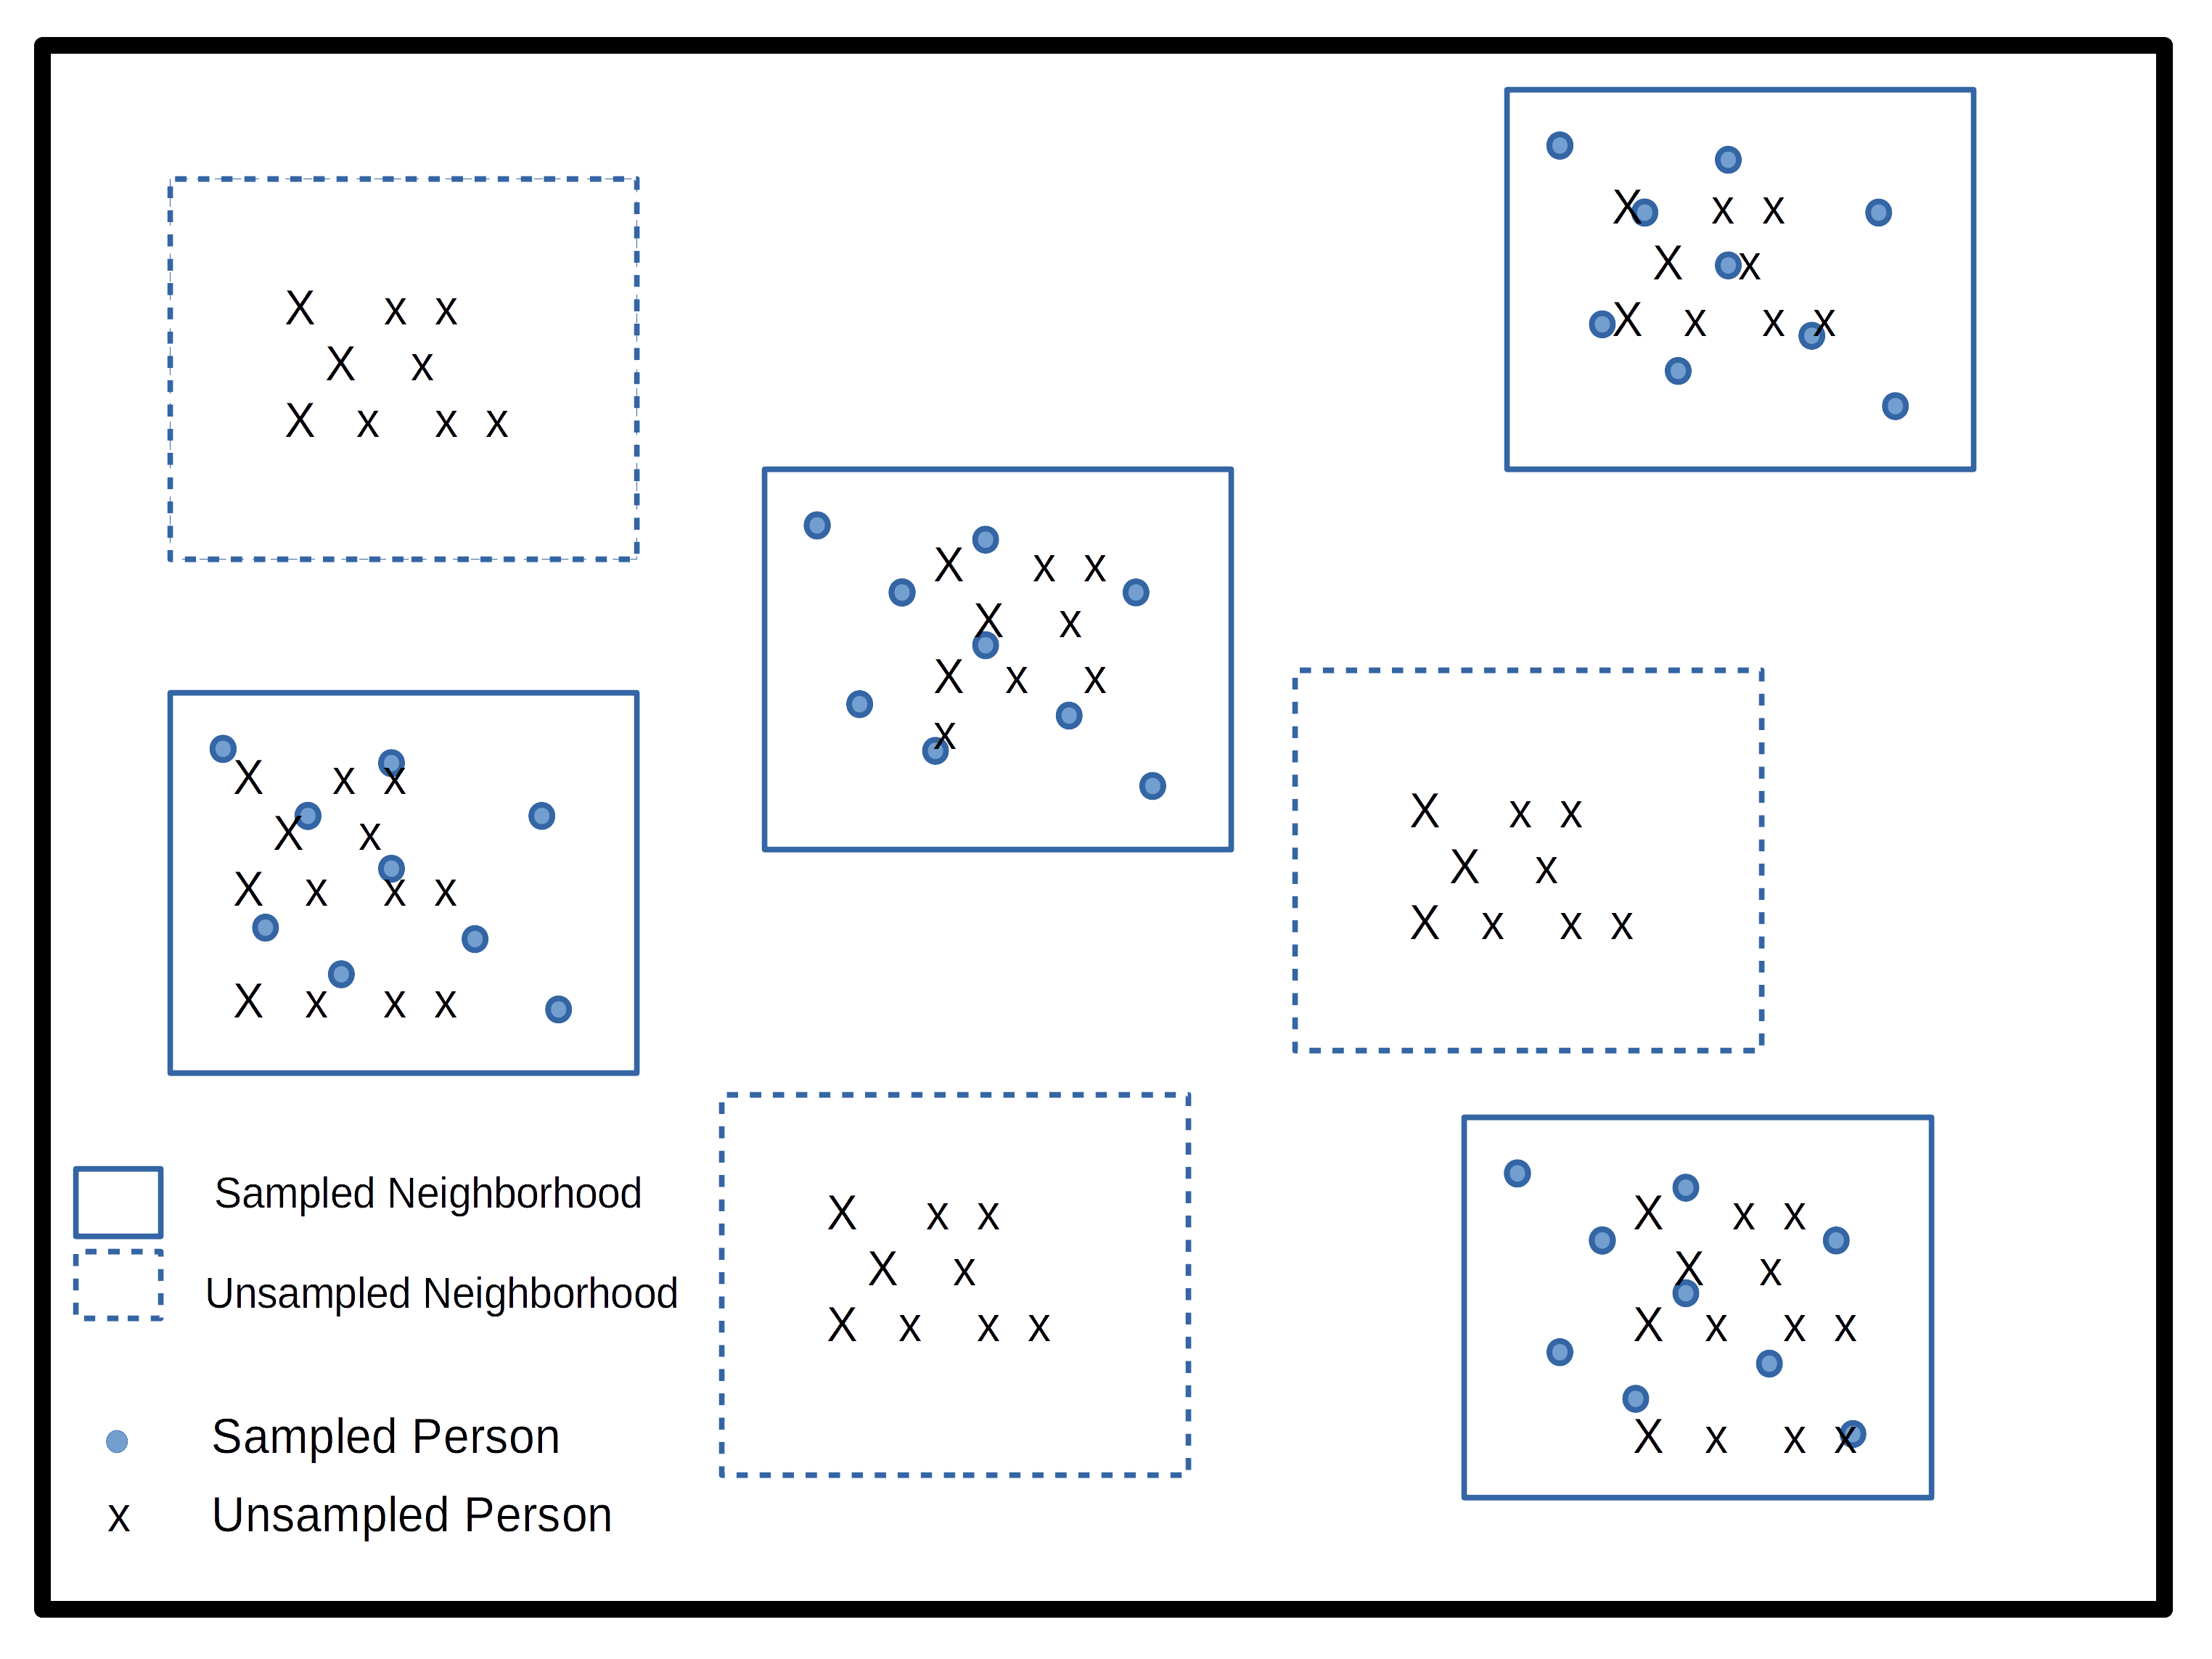
\includegraphics{images/MLdata.png}

}

\caption{Figure 1}

\end{figure}

\hypertarget{simple-versus-complex-survey-designs}{%
\section{Simple versus complex survey
designs}\label{simple-versus-complex-survey-designs}}

How the data we're using is sampled has a major implication for how we
analyze it. The majority of statistical tools assume that data come from
simple random samples, because most methods assume independence of
observations, regardless of which distribution or test statistic you are
using. Violations of this assumption are a big problem when we go to
analyze our data, because the non-independence of survey data are
automatically in violation of a key assumption of any test. The
stratified and clustered nature of many survey samples may also present
problems for methods such as linear regression analysis which assume
errors in the model are \textbf{homoskedastic}, or constant. When data
are collected in a stratified or clustered method, the data may have
less variation than a simple random sample, because individuals who live
closely to one another often share other characteristics in common as
well. Our statistical models don't do well with this type of reduction
in variation and we often have to resort to manipulations of our model
parameters or standard errors of our statistics in order to make them
coincide with how the data were collected.

Not to fear! Data collected using public funds are typically required to
be made available to the public with information on how to use them.
Most surveys come with some kind of code book or user manual which
describes how the data were collected and how you should go about using
them. In these cases, it pays to read the manual because it will tell
you the names of the stratification and clustering variables in the
survey data. This will allow you to use the design of the survey in your
analysis so that your statistical routines are corrected for the
non-randomness and homogeneity in the survey data.

\textbf{He's not heavy, he's my brother}

Another important aspect of survey data are the use of weighting
variables. Whenever we design a survey, we have our target population,
or universe of respondents in mind. In the DHS, again, this is
traditionally\footnote{The modern DHS collects information on couples,
  men and children, so the universe has been expanded away from just
  women of childbearing age and their children.} women of childbearing
age and their children (International 2012). When we collect a sample
from this population, or sample may be, and typically is, imperfect. It
is imperfect for many reasons, owing to the difficulty of sampling some
members of the population, or their unwillingness to participate in our
study. Part of designing an effective survey is knowing your universe or
population, and its characteristics. This will let you know the
probability of a particular person being in the sample. Of course, the
more complicated the survey, the more complicated it is to know what
this probability is. For example, if we were to sample people in the
United States, using a stratified design based on rural and urban
residence, we would need to know how many people lived in rural and
urban areas within the country, as this would effect the probability of
sampling a person in each type of area. This \textbf{inclusion
probability} tells us how likely a given person is of being sampled. The
inverse of the inclusion probability is called the \textbf{sampling
weight}:

\(w_i = \frac{1} {\pi_i}\)

where \(\pi_i\) is the inclusion probability.

Sampling weights are what we use to make our analyses of a survey
representative of the larger population. They serve many purposes
including unequal inclusion probabilities, differences in sample
characteristics compared to the larger population, and differences in
response rates across sample subgroups. All of these situations make the
sample deviate from the population by affecting who the actual
respondents included in the survey are. Differences in our sample when
compared to the larger population can affect most all of our statistical
analysis since again, most methods assume random sampling. The weights
that are included in public data are the result of a rigorous process
conducted by those who designed and implemented the survey itself, and
most surveys in their user manuals or code books describe the process of
how the weights are created. For example, the US Center for Disease
Control and Prevention's Behavioral Risk Factor Surveillance System
(BRFSS) provides a very thorough description of how their final person
weights are calculated (CDC 2020). These weights include three primary
factors, the \emph{stratum weight}, which is a combination of the number
of records in a sample strata and the density of phone lines in a given
strata, combined with the number of phones in a sampled household and
the number of adults in the household to produce the final design
weight. These weights are then \textbf{raked} to eight different
marginal totals, based on age, race/ethnicity, education, marital
status, home ownership, gender by race/ethnicity, age by race/ethnicity
and phone ownership(CDC 2020). After this process, weights are
interpretable as the number of people a given respondent in the survey
represents in the population. So, if a respondent's weight in the survey
data is 100, they actually represent 100 people in the target
population.

Other types of weights also exist, and are commonly seen in federal data
sources. A common kind of weight that includes information on both the
probability of inclusion \textbf{AND} the stratified design of the
survey are \textbf{replicate weights}. Replicate weights are multiple
weights for each respondent, and there are as many weights as there are
different levels of the stratification variable. Later in this chapter,
we will discuss how replicate weights are used, as compared to single
design weights in an example.

\hypertarget{characteristics-of-your-survey}{%
\section{Characteristics of YOUR
survey}\label{characteristics-of-your-survey}}

Survey data that come from reputable sources, such as most federal
agencies or repositories such as the Inter-university Consortium for
Political and Social Research (ICPSR) at the University of Michigan in
the United States, are accompanied by descriptions of the data source
including when and where it was collected, what it's target population
is, and information on the design of the survey. This will include
information on sample design, such as stratum or cluster variables, and
design or replicate weights to be used when you conduct your analysis. I
cannot stress enough that learning how your particular survey data
source is designed, and how the designers recommend you use provided
survey variables for your analysis, is imperative to ensure your
analysis is correctly specified.

\hypertarget{example-from-the-american-community-survey}{%
\section{Example from the American Community
Survey}\label{example-from-the-american-community-survey}}

Let's look at an example of these ideas in a real data source.
Throughout the book I will use several complex survey design data
sources to illustrate various topics, in this chapter I will use data
from the US Census Bureau's American Community Survey (ACS) public use
microdata sample (PUMS). We can actually use the \texttt{tidycensus}
package (Walker and Herman 2021) to download ACS PUMS directly from the
Census Bureau.

This example shows how to extract the 2018 single-year PUMS for the
state of Texas, and only keep variables related to person-records. The
ACS has information on both people and households, but for now we'll
only look at the person records. Help on these functions can be found by
typing \texttt{?pums\_variables} and \texttt{?get\_pums} in \texttt{R}

\begin{Shaded}
\begin{Highlighting}[]
\FunctionTok{library}\NormalTok{(tidycensus)}
\FunctionTok{library}\NormalTok{(tidyverse)}

\NormalTok{pums\_vars\_18}\OtherTok{\textless{}{-}}\NormalTok{ pums\_variables }\SpecialCharTok{\%\textgreater{}\%}
  \FunctionTok{filter}\NormalTok{(year}\SpecialCharTok{==} \DecValTok{2018}\NormalTok{, survey }\SpecialCharTok{==} \StringTok{"acs1"}\NormalTok{) }\SpecialCharTok{\%\textgreater{}\%}
  \FunctionTok{distinct}\NormalTok{(var\_code, var\_label, data\_type, level) }\SpecialCharTok{\%\textgreater{}\%}
  \FunctionTok{filter}\NormalTok{(level }\SpecialCharTok{==} \StringTok{"person"}\NormalTok{)}

\NormalTok{TX\_pums }\OtherTok{\textless{}{-}} \FunctionTok{get\_pums}\NormalTok{(}
  \AttributeTok{variables =} \FunctionTok{c}\NormalTok{(}\StringTok{"PUMA"}\NormalTok{, }\StringTok{"SEX"}\NormalTok{, }\StringTok{"AGEP"}\NormalTok{, }\StringTok{"CIT"}\NormalTok{, }\StringTok{"JWTR"}\NormalTok{,}\StringTok{"JWRIP"}\NormalTok{, }\StringTok{"HISP"}\NormalTok{),}
  \AttributeTok{state =} \StringTok{"AL"}\NormalTok{,}
  \AttributeTok{survey =} \StringTok{"acs1"}\NormalTok{,}
  \AttributeTok{year =} \DecValTok{2018}\NormalTok{)}
\end{Highlighting}
\end{Shaded}

\begin{Shaded}
\begin{Highlighting}[]
\NormalTok{knitr}\SpecialCharTok{::}\FunctionTok{kable}\NormalTok{(}
  \FunctionTok{head}\NormalTok{(TX\_pums),}
  \AttributeTok{format =} \StringTok{\textquotesingle{}html\textquotesingle{}}
\NormalTok{  )}
\end{Highlighting}
\end{Shaded}

These data are also easily available from the Integrated Public Use
Microdata Series (IPUMS) project housed at the University of Minnesota
(Ruggles et al. 2021). The IPUMS version of the data adds additional
information to the data and homogenizes the data across multiple years
to make using it easier. The following example will use the
\texttt{ipumsr} package to read in an extract from IPUMS-USA.

After you create an IPUMS extract, right click on the DDI link and save
that file to your computer. Then repeat this for the .DAT file. If you
need help creating an IPUMS extract, their staff have created a tutorial
for doing so (\url{https://usa.ipums.org/usa/tutorials.shtml}).

This will save the xml file that contains all the information on the
data (what is contained in the data file) to your computer. When using
IPUMS, it will have a name like \texttt{usa\_xxxxx.xml} where the x's
represent the extract number.

You will also need to download the data file, by right clicking the
\textbf{Download.DAT} link in the above image. This will save a .gz file
to your computer, again with a name like: \texttt{usa\_xxxxx.dat.gz}.
Make sure this file and the xml file from above are in the same folder.

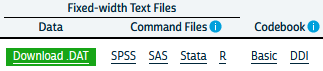
\includegraphics{images/impum1.png}

The fundamentals of using \texttt{ipumsr} is to specify the name of your
\texttt{.xml} file from your extract, and as long as your
\texttt{.tar.gz} file from your extract is in the same location, R will
read the data. The files on my computer:

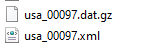
\includegraphics{images/ipums_files.png}

\begin{Shaded}
\begin{Highlighting}[]
\FunctionTok{library}\NormalTok{(ipumsr)}

\NormalTok{ddi }\OtherTok{\textless{}{-}} \FunctionTok{read\_ipums\_ddi}\NormalTok{(}\AttributeTok{ddi\_file =} \StringTok{"data/usa\_00097.xml"}\NormalTok{)}
\NormalTok{ipums }\OtherTok{\textless{}{-}} \FunctionTok{read\_ipums\_micro}\NormalTok{(}\AttributeTok{ddi =}\NormalTok{ ddi)}
\end{Highlighting}
\end{Shaded}

Will read in the data, in this case, it is a subset of the 2008 to 2012
single year ACS. This extract is not all of the variables from the ACS,
as that would be a very large file and for my purposes here, I don't
need that. My goal for the rest of the chapter is to illustrate how to
use the IPUMS as an example of a complex survey design data set and the
steps necessary to do so.

\hypertarget{basics-of-analyzing-survey-data}{%
\section{Basics of analyzing survey
data}\label{basics-of-analyzing-survey-data}}

A fundamental part of analyzing complex survey data are knowing the
variables within the data that contain the survey design information.
The US Census Bureau has documented the design of the survey in a
publication (US Census Bureau 2014) The IPUMS version of the ACS has two
variables \texttt{STRATA} and \texttt{CLUSTER} that describe the two
stage process by which the data are collected. Here are a the first few
lines of these from the data:

\begin{Shaded}
\begin{Highlighting}[]
\FunctionTok{options}\NormalTok{(}\AttributeTok{scipen =} \DecValTok{999}\NormalTok{)}
\FunctionTok{library}\NormalTok{(knitr)}
  
\FunctionTok{kable}\NormalTok{(}\FunctionTok{head}\NormalTok{(ipums[, }\FunctionTok{c}\NormalTok{(}\StringTok{"SERIAL"}\NormalTok{, }\StringTok{"STRATA"}\NormalTok{, }\StringTok{"CLUSTER"}\NormalTok{)],}
           \AttributeTok{n=}\DecValTok{10}\NormalTok{),}
      \AttributeTok{digits =} \DecValTok{14}\NormalTok{ )}
\end{Highlighting}
\end{Shaded}

For the ACS, the strata variable is named, ironically \texttt{STRATA}
and the cluster variable \texttt{CLUSTER}. The IPUMS creates the
\texttt{STRATA} variable based on the sampling strata in the ACS, and
the \texttt{CLUSTER} variable based on households within a stratum.
Often in surveys, the clusters may not be households, they could be
smaller population aggregates, such as neighborhoods and villages, as in
the DHS.

The data also come with housing unit weights and person unit weights, so
your analysis can be either representative of housing units or people.

\begin{Shaded}
\begin{Highlighting}[]
\FunctionTok{kable}\NormalTok{(}\FunctionTok{head}\NormalTok{(ipums[, }\FunctionTok{c}\NormalTok{(}\StringTok{"SERIAL"}\NormalTok{, }\StringTok{"STRATA"}\NormalTok{, }\StringTok{"CLUSTER"}\NormalTok{, }\StringTok{"HHWT"}\NormalTok{, }\StringTok{"PERWT"}\NormalTok{)],}
           \AttributeTok{n=}\DecValTok{10}\NormalTok{),}
      \AttributeTok{digits =} \DecValTok{14}\NormalTok{ )}
\end{Highlighting}
\end{Shaded}

\begin{longtable}[]{@{}rrrrr@{}}
\toprule\noalign{}
SERIAL & STRATA & CLUSTER & HHWT & PERWT \\
\midrule\noalign{}
\endhead
\bottomrule\noalign{}
\endlastfoot
1189369 & 330148 & 2019011893691 & 67 & 67 \\
1189370 & 231948 & 2019011893701 & 43 & 43 \\
1189371 & 690048 & 2019011893711 & 114 & 114 \\
1189372 & 430248 & 2019011893721 & 34 & 34 \\
1189373 & 650048 & 2019011893731 & 35 & 35 \\
1189374 & 680548 & 2019011893741 & 19 & 19 \\
1189375 & 340048 & 2019011893751 & 18 & 18 \\
1189376 & 60048 & 2019011893761 & 37 & 37 \\
1189377 & 440048 & 2019011893771 & 76 & 76 \\
1189378 & 462348 & 2019011893781 & 10 & 10 \\
\end{longtable}

As can be seen in the first few cases, the \texttt{HHWT} variable is the
same for everyone in a given household, but each person has a unique
person weight showing that they each represent different numbers of
people in the population. Further investigation of the housing and
person weights allow us to see what these values actually look like.

\begin{Shaded}
\begin{Highlighting}[]
\FunctionTok{summary}\NormalTok{(ipums}\SpecialCharTok{$}\NormalTok{PERWT)}
\end{Highlighting}
\end{Shaded}

\begin{verbatim}
   Min. 1st Qu.  Median    Mean 3rd Qu.    Max. 
    1.0    49.0    78.0   106.3   128.0  2376.0 
\end{verbatim}

Here we see the minimum person weight is 1 and the maximum is 2376,
which tells us that at least on person in the data represents 2376
people in the population that year. A histogram of the weights can also
show us the distribution of weights in the sample.

\begin{Shaded}
\begin{Highlighting}[]
\FunctionTok{library}\NormalTok{(ggplot2)}

\NormalTok{ipums}\SpecialCharTok{\%\textgreater{}\%}
  \FunctionTok{ggplot}\NormalTok{(}\FunctionTok{aes}\NormalTok{(}\AttributeTok{x =}\NormalTok{ PERWT)) }\SpecialCharTok{+}
    \FunctionTok{geom\_histogram}\NormalTok{() }\SpecialCharTok{+} 
  \FunctionTok{labs}\NormalTok{(}\AttributeTok{title =} \StringTok{"Histogram of ACS Person Weights, 2019"}\NormalTok{)}
\end{Highlighting}
\end{Shaded}

\begin{figure}[H]

{\centering 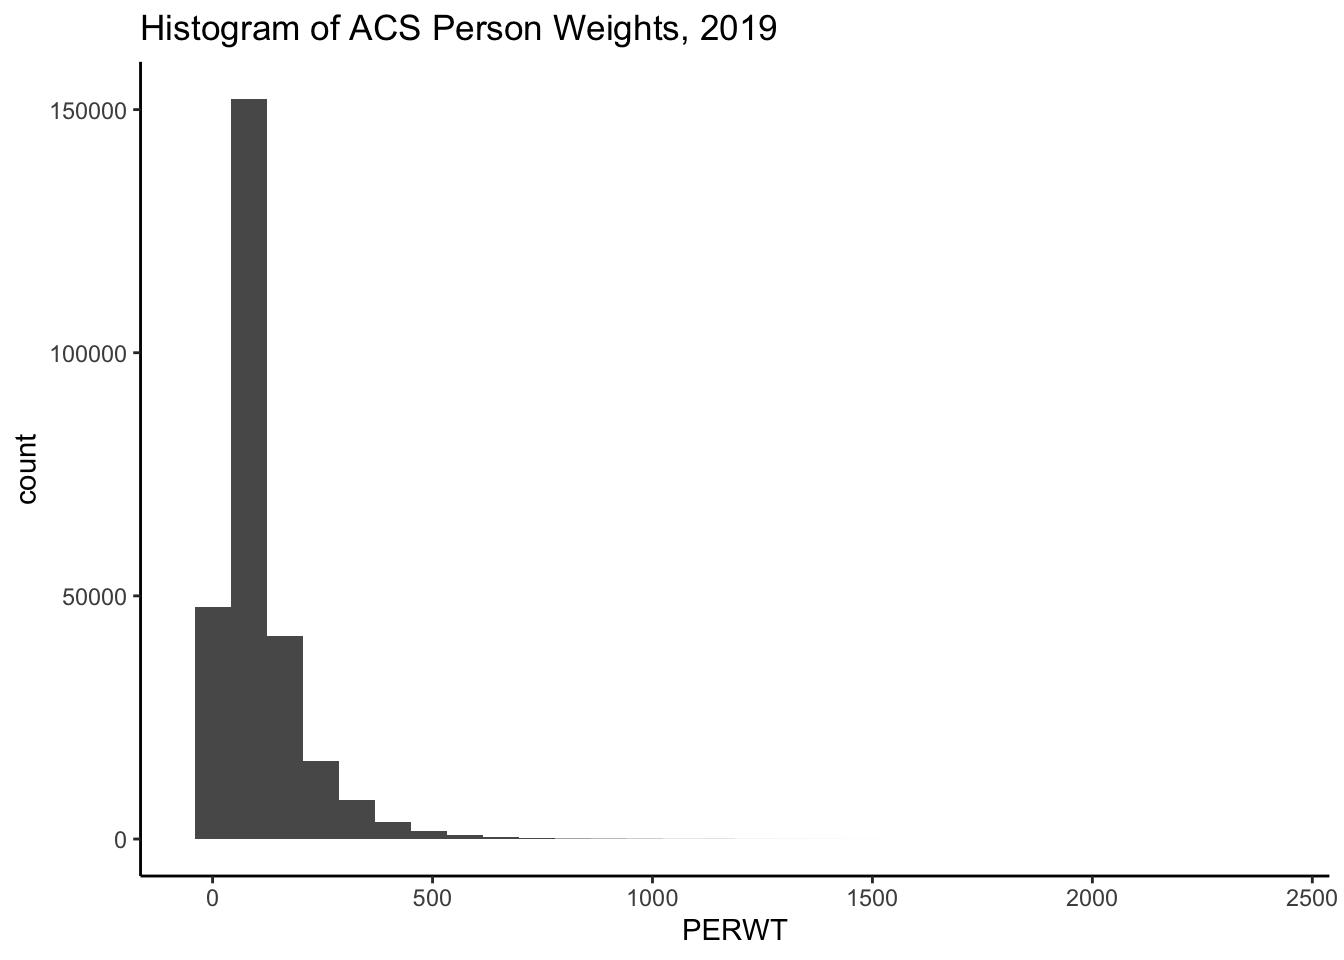
\includegraphics{survey_files/figure-pdf/unnamed-chunk-7-1.pdf}

}

\end{figure}

We can see how the weights inflate each person or household to the
population by summing the weights. Below, I sum the person weights for
the state of Texas, the sum is 28,995,881 million people, which is the
same as the official estimate of the population in 2019
(\url{https://www.census.gov/quickfacts/TX}), we also see, by using the
\texttt{n()} function, that there were 272,776 persons in the sample in
2019 living in Texas.

\begin{Shaded}
\begin{Highlighting}[]
\FunctionTok{library}\NormalTok{(dplyr)}
\NormalTok{ipums}\SpecialCharTok{\%\textgreater{}\%}
  \FunctionTok{filter}\NormalTok{(STATEFIP }\SpecialCharTok{==} \DecValTok{48}\NormalTok{)}\SpecialCharTok{\%\textgreater{}\%}
  \FunctionTok{summarize}\NormalTok{(}\AttributeTok{tot\_pop =} \FunctionTok{sum}\NormalTok{( PERWT ) , }\AttributeTok{n\_respond =} \FunctionTok{n}\NormalTok{())}
\end{Highlighting}
\end{Shaded}

\begin{verbatim}
# A tibble: 1 x 2
   tot_pop n_respond
     <dbl>     <int>
1 28995881    272776
\end{verbatim}

For housing units, we have to select a single person from the household
in order for the same process to work, otherwise we would misrepresent
the number of households in the state. We see there are 10,585,803
million housing units, and 114,016 unique households in the data.

\begin{Shaded}
\begin{Highlighting}[]
\NormalTok{ipums}\SpecialCharTok{\%\textgreater{}\%}
  \FunctionTok{filter}\NormalTok{(STATEFIP }\SpecialCharTok{==} \DecValTok{48}\NormalTok{,}
\NormalTok{         PERNUM }\SpecialCharTok{==} \DecValTok{1}\NormalTok{)}\SpecialCharTok{\%\textgreater{}\%}
  \FunctionTok{summarize}\NormalTok{(}\AttributeTok{tothh =} \FunctionTok{sum}\NormalTok{( HHWT ) , }\AttributeTok{n\_housing =} \FunctionTok{n}\NormalTok{())}
\end{Highlighting}
\end{Shaded}

\begin{verbatim}
# A tibble: 1 x 2
     tothh n_housing
     <dbl>     <int>
1 10585803    114016
\end{verbatim}

This total is nearly identical to that from the
\href{https://data.census.gov/cedsci/table?t=Housing\&g=0400000US48\&y=2019\&tid=ACSDP1Y2019.DP04}{Census's
ACS estimate}.

This exercise shows that by using the provided weights in the survey, we
can estimate the population size the sample was supposed to capture
effectively. The \texttt{survey} package and the newer tidyverse package
\texttt{srvyr} are designed to fully implement survey design and
weighting and perform a wide variety of statistical summaries.

The way these packages work, is that you provide the name of your data
frame, and the survey design variables that are in your data and the
package code performs the requested analysis, correcting for survey
design and weighting to the appropriate population. The code below
illustrates how to enter the survey design for the IPUMS-USA ACS. Some
surveys will not have both a cluster and stratification variable, so
again, it's important to consult your survey documentation to find these
for your data.

The function \texttt{as\_survey\_design()} in this case takes three
arguments, since we are piping the 2019 ACS into it, we don't have to
specify the name of the data. \texttt{ids} is the argument for the
cluster variable, if your survey doesn't have one, just leave it out.
\texttt{strata} is where you specify the name of the survey
stratification variable, and \texttt{weights} is where you specify the
name of the appropriate weighting variable. In this case, I'm
replicating the estimate of the housing units in Texas from above, so
I'll use the \texttt{HHWT} variable. The easiest way to get a total
population estimate is to use the \texttt{survey\_total()} function,
which is equivalent to summing the weights as shown above, although in
the case of the survey analysis commands in the \texttt{survey} and
\texttt{srvyr} packages, the total will also be estimated with a
standard error of the estimate.

\begin{Shaded}
\begin{Highlighting}[]
\FunctionTok{library}\NormalTok{(srvyr)}
\FunctionTok{library}\NormalTok{(survey)}

\NormalTok{ipums}\SpecialCharTok{\%\textgreater{}\%}
  \FunctionTok{filter}\NormalTok{(STATEFIP }\SpecialCharTok{==} \DecValTok{48}\NormalTok{, PERNUM }\SpecialCharTok{==} \DecValTok{1}\NormalTok{)}\SpecialCharTok{\%\textgreater{}\%}
  \FunctionTok{as\_survey\_design}\NormalTok{(}\AttributeTok{cluster=}\NormalTok{ CLUSTER,}
                   \AttributeTok{strata =}\NormalTok{ STRATA,}
                   \AttributeTok{weights =}\NormalTok{ HHWT)}\SpecialCharTok{\%\textgreater{}\%}
  \FunctionTok{summarize}\NormalTok{(}\AttributeTok{tothh =} \FunctionTok{survey\_total}\NormalTok{())}
\end{Highlighting}
\end{Shaded}

\textbf{A short aside about survey design options} The core definition
of the ACS survey design is shown in the code above, and I highly
recommend that you inspect the help file for the survey design functions
\texttt{?as\_survey\_design} or \texttt{?svydesign}. An important option
that often has to be specified is the \texttt{nest=TRUE} option. This if
often necessary if PSU identifiers are not unique across strata. For
example, the fictional data shown below has the PSU's values the same
across strata.\}

\begin{Shaded}
\begin{Highlighting}[]
\NormalTok{fake\_survey}\OtherTok{\textless{}{-}} \FunctionTok{data.frame}\NormalTok{(}
  \AttributeTok{strata =} \FunctionTok{c}\NormalTok{(}\DecValTok{1}\NormalTok{,}\DecValTok{1}\NormalTok{,}\DecValTok{1}\NormalTok{,}\DecValTok{1}\NormalTok{,}\DecValTok{1}\NormalTok{,}\DecValTok{1}\NormalTok{,}
             \DecValTok{2}\NormalTok{,}\DecValTok{2}\NormalTok{,}\DecValTok{2}\NormalTok{,}\DecValTok{2}\NormalTok{,}\DecValTok{2}\NormalTok{,}\DecValTok{2}\NormalTok{),}
  \AttributeTok{psu =} \FunctionTok{c}\NormalTok{(}\DecValTok{1}\NormalTok{,}\DecValTok{1}\NormalTok{,}\DecValTok{1}\NormalTok{,}\DecValTok{2}\NormalTok{,}\DecValTok{2}\NormalTok{,}\DecValTok{3}\NormalTok{,}
          \DecValTok{1}\NormalTok{,}\DecValTok{1}\NormalTok{,}\DecValTok{2}\NormalTok{,}\DecValTok{2}\NormalTok{,}\DecValTok{3}\NormalTok{,}\DecValTok{3}\NormalTok{),}
  \AttributeTok{weight =} \FunctionTok{rpois}\NormalTok{(}\AttributeTok{n =} \DecValTok{12}\NormalTok{, }\AttributeTok{lambda =} \DecValTok{20}\NormalTok{))}

\NormalTok{knitr}\SpecialCharTok{::}\FunctionTok{kable}\NormalTok{(fake\_survey)}
\end{Highlighting}
\end{Shaded}

\begin{longtable}[]{@{}rrr@{}}
\toprule\noalign{}
strata & psu & weight \\
\midrule\noalign{}
\endhead
\bottomrule\noalign{}
\endlastfoot
1 & 1 & 15 \\
1 & 1 & 22 \\
1 & 1 & 13 \\
1 & 2 & 25 \\
1 & 2 & 26 \\
1 & 3 & 23 \\
2 & 1 & 19 \\
2 & 1 & 19 \\
2 & 2 & 16 \\
2 & 2 & 30 \\
2 & 3 & 16 \\
2 & 3 & 19 \\
\end{longtable}

If we attempt to make a survey design from this, R would show an error.

\begin{Shaded}
\begin{Highlighting}[]
\NormalTok{fake\_design}\OtherTok{\textless{}{-}}\NormalTok{ fake\_survey}\SpecialCharTok{\%\textgreater{}\%}
  \FunctionTok{as\_survey\_design}\NormalTok{(}\AttributeTok{ids =}\NormalTok{ psu,}
                    \AttributeTok{strata=}\NormalTok{strata,}
                    \AttributeTok{weights =}\NormalTok{ weight)}
\end{Highlighting}
\end{Shaded}

\begin{verbatim}
Error in svydesign.default(ids, probs, strata, variables, fpc, .data, : Clusters not nested in strata at top level; you may want nest=TRUE.
\end{verbatim}

But if we include the \texttt{nest\ =\ TRUE} option, R doesn't give us
the error:

\begin{Shaded}
\begin{Highlighting}[]
\NormalTok{fake\_design}\OtherTok{\textless{}{-}}\NormalTok{ fake\_survey}\SpecialCharTok{\%\textgreater{}\%}
  \FunctionTok{as\_survey\_design}\NormalTok{(}\AttributeTok{ids =}\NormalTok{ psu,}
                  \AttributeTok{strata=}\NormalTok{strata,}
                  \AttributeTok{weights =}\NormalTok{ weight, }
                  \AttributeTok{nest =} \ConstantTok{TRUE}\NormalTok{)}
\NormalTok{fake\_design}
\end{Highlighting}
\end{Shaded}

\begin{verbatim}
Stratified 1 - level Cluster Sampling design (with replacement)
With (6) clusters.
Called via srvyr
Sampling variables:
 - ids: psu
 - strata: strata
 - weights: weight
Data variables: strata (dbl), psu (dbl), weight (int)
\end{verbatim}

The ACS from IPUMS has unique CLUSTERs across strata, so we don't have
to specify that argument when we declare our survey design.

Back to our housing estimates.

In this case, our \texttt{tothh} estimate is identical to summing the
weights, but new we also have an estimate of the precision of the
estimate, so we could produce a more informed statistical estimate that
in 2019, there were 10,585,803 \(\pm\) 27,274.96 occupied housing units
in the state.

If your data come with replicate weights instead of strata and cluster
variables, this can be specified using the \texttt{as\_survey\_rep()}
command instead \texttt{as\_survey\_design()}. In this case, we have to
specify all of the columns which correspond to the replicate weights in
the data. There are likely many ways to do this, but below, I use a
method that matches the column names using a regular expression, where
we are looking for the string \texttt{REPWT}, followed by any number of
numeric digits, that is what the \texttt{{[}0-9{]}+} portion tells R to
do. Also, the ACS uses a balanced replicate weight construction, which
also requires the case weight as well (Ruggles et al. 2021), so we
specify the replicate weight type as \texttt{BRR}. Again, this is
specific to the ACS, and you need to consult your own code book for your
survey for your design information.

In this case, we get the same estimate for the total number of housing
units, but a smaller variance in the estimate, which is often seen when
using replicate weights.

\begin{Shaded}
\begin{Highlighting}[]
\NormalTok{ipums}\SpecialCharTok{\%\textgreater{}\%}
  \FunctionTok{filter}\NormalTok{(STATEFIP }\SpecialCharTok{==} \DecValTok{48}\NormalTok{, PERNUM }\SpecialCharTok{==} \DecValTok{1}\NormalTok{)}\SpecialCharTok{\%\textgreater{}\%}
  \FunctionTok{as\_survey\_rep}\NormalTok{(}\AttributeTok{weight =}\NormalTok{ HHWT,}
            \AttributeTok{repweights =}\FunctionTok{matches}\NormalTok{(}\StringTok{"REPWT[0{-}9]+"}\NormalTok{),}
            \AttributeTok{type =} \StringTok{"JK1"}\NormalTok{,}
            \AttributeTok{scale =} \DecValTok{4}\SpecialCharTok{/}\DecValTok{80}\NormalTok{,}
            \AttributeTok{rscales =} \FunctionTok{rep}\NormalTok{(}\DecValTok{1}\NormalTok{, }\DecValTok{80}\NormalTok{),}
            \AttributeTok{mse =} \ConstantTok{TRUE}\NormalTok{)}\SpecialCharTok{\%\textgreater{}\%}
  \FunctionTok{summarize}\NormalTok{(}\AttributeTok{tothh =} \FunctionTok{survey\_total}\NormalTok{())}
\end{Highlighting}
\end{Shaded}

\begin{verbatim}
# A tibble: 1 x 2
     tothh tothh_se
     <dbl>    <dbl>
1 10585803   15479.
\end{verbatim}

\begin{Shaded}
\begin{Highlighting}[]
\NormalTok{rw}\OtherTok{\textless{}{-}}\NormalTok{ipums}\SpecialCharTok{\%\textgreater{}\%}
      \FunctionTok{filter}\NormalTok{(STATEFIP}\SpecialCharTok{==}\DecValTok{48}\NormalTok{, PERNUM}\SpecialCharTok{==}\DecValTok{1}\NormalTok{)}\SpecialCharTok{\%\textgreater{}\%}
      \FunctionTok{select}\NormalTok{(REPWT1}\SpecialCharTok{:}\NormalTok{REPWT50)}

\NormalTok{t1}\OtherTok{\textless{}{-}}\NormalTok{survey}\SpecialCharTok{::}\FunctionTok{svrepdesign}\NormalTok{(}\AttributeTok{data=}\NormalTok{ipums[ipums}\SpecialCharTok{$}\NormalTok{STATEFIP}\SpecialCharTok{==}\DecValTok{48}\SpecialCharTok{\&}\NormalTok{ipums}\SpecialCharTok{$}\NormalTok{PERNUM}\SpecialCharTok{==}\DecValTok{1}\NormalTok{,],}
                        \AttributeTok{repweights =}\NormalTok{ rw,}
                        \AttributeTok{weights =}\NormalTok{ ipums}\SpecialCharTok{$}\NormalTok{HHWT[ipums}\SpecialCharTok{$}\NormalTok{STATEFIP}\SpecialCharTok{==}\DecValTok{48}\SpecialCharTok{\&}\NormalTok{ipums}\SpecialCharTok{$}\NormalTok{PERNUM}\SpecialCharTok{==}\DecValTok{1}\NormalTok{],}
                        \AttributeTok{type=}\StringTok{"JK1"}\NormalTok{,}\AttributeTok{scale =}\NormalTok{ .}\DecValTok{05}\NormalTok{, }\AttributeTok{rscales =} \FunctionTok{rep}\NormalTok{(}\DecValTok{1}\NormalTok{, }\FunctionTok{ncol}\NormalTok{(rw)), }\AttributeTok{mse=} \ConstantTok{TRUE}\NormalTok{)}

\NormalTok{t1}\SpecialCharTok{$}\NormalTok{variables}\SpecialCharTok{$}\NormalTok{ones}\OtherTok{\textless{}{-}}\DecValTok{1}
\FunctionTok{library}\NormalTok{(survey)}

\FunctionTok{svytotal}\NormalTok{(}\SpecialCharTok{\textasciitilde{}}\NormalTok{ones, }\AttributeTok{design=}\NormalTok{t1)}
\end{Highlighting}
\end{Shaded}

\begin{verbatim}
        total    SE
ones 10585803 11850
\end{verbatim}

We can also define the survey design outside of a dplyr pipe if we want
using the \texttt{survey} package.

\begin{Shaded}
\begin{Highlighting}[]
\NormalTok{acs\_design }\OtherTok{\textless{}{-}} \FunctionTok{svydesign}\NormalTok{(}\AttributeTok{ids =} \SpecialCharTok{\textasciitilde{}}\NormalTok{ CLUSTER, }
                        \AttributeTok{strata=} \SpecialCharTok{\textasciitilde{}}\NormalTok{ STRATA, }
                        \AttributeTok{weights =} \SpecialCharTok{\textasciitilde{}}\NormalTok{ PERWT, }
                        \AttributeTok{data=}\NormalTok{ipums)}

\NormalTok{acs\_design}
\end{Highlighting}
\end{Shaded}

\begin{verbatim}
Stratified 1 - level Cluster Sampling design (with replacement)
With (114016) clusters.
svydesign(ids = ~CLUSTER, strata = ~STRATA, weights = ~PERWT, 
    data = ipums)
\end{verbatim}

Of course we typically want to do more analysis than just estimate a
population size, and typically we are interested in using survey data
for comparisons and regression modeling. To carry out any sort of
statistical testing on survey data, we must not only weight the data
appropriately but we must also calculate all measures of variability
correctly as well. Since surveys are stratified, the traditional formula
for variances is not correct because under stratified sampling, all
estimates are not only a function of the total sample, but also the
within-strata sample averages and sample sizes. We can estimate the
variances in our estimates using the design variables and sample weights
in the survey analysis procedures, but there are options.

\hypertarget{replicates-and-jack-knifes-and-expansions-oh-my}{%
\section{Replicates and jack knifes and expansions, oh
my!}\label{replicates-and-jack-knifes-and-expansions-oh-my}}

When conducting your analysis, you may not have any choices of whether
you should use replicate weights or design weights, because your survey
may only have one of these. There are two main strategies to estimate
variances in survey data, the \emph{Taylor Series Approximation} also
referred to as \emph{linearization} and the use of \emph{replicate
weights}. The Taylor Series, or linearization method is an approximation
to the true variance, but is likely the most commonly used technique
when analyzing survey data using regression methods. Lohr (2019)
describes the calculation of variances from simple and clustered random
samples in her book, and by her admission, once one has a clustered
random sample the variance calculations for simple calculations becomes
much more complex.

The problem is that we often want much more complicated calculations in
our work and the variance formulas for anything other than simple ratios
are not analytically known. The Taylor series approximation to the
variance for complex and nonlinear terms such as ratios or estimates of
regression parameters. The \texttt{survey} package in R will do this if
you specify a survey design that includes strata or clusters, while if
you specify replicate weights then it will use an appropriate technique
depending on how the data were collected.

Typical replicate methods include balanced replicates, where there are
exactly two clusters within each stratum, jackknife methods, which
effectively remove one cluster from the strata and perform all
calculations without that cluster in the analysis, then average across
all replicates, and bootstrap methods which randomly sample clusters
within strata with replacement a large number of times to get an
estimate of the quantities of interest.

\hypertarget{descriptive-analysis-of-survey-data}{%
\section{Descriptive analysis of survey
data}\label{descriptive-analysis-of-survey-data}}

The \texttt{survey} library allows many forms of descriptive and
regression analysis.

\hypertarget{weighted-frequencies-and-rates}{%
\section{Weighted frequencies and
rates}\label{weighted-frequencies-and-rates}}

Basic frequency tables are very useful tools for examining bivariate
associations in survey data. In the survey analysis packages in R, the
basic tools for doing this are the \texttt{svytable()} function in
\texttt{survey}, or via the \texttt{survey\_total()} function in
\texttt{srvyr}. First I will recode two variables in the ACS, the
employment status to indicate if a respondent is currently employed, and
the \texttt{MET2013} variable, which is the metropolitan area where the
respondent was living. This will give us the ACS estimate for the
employed and unemployed population in each Texas MSA. I first have to
filter the data to be people of working age, who are in the labor force
and living in a MSA.

\begin{Shaded}
\begin{Highlighting}[]
\NormalTok{ipums }\SpecialCharTok{\%\textgreater{}\%}
  \FunctionTok{filter}\NormalTok{(EMPSTAT }\SpecialCharTok{\%in\%} \DecValTok{1}\SpecialCharTok{:}\DecValTok{2}\NormalTok{,}
\NormalTok{         AGE }\SpecialCharTok{\textgreater{}=} \DecValTok{16} \SpecialCharTok{\&}\NormalTok{ AGE }\SpecialCharTok{\textless{}=} \DecValTok{65}\NormalTok{, }
\NormalTok{         MET2013 }\SpecialCharTok{!=} \DecValTok{0}\NormalTok{) }\SpecialCharTok{\%\textgreater{}\%}
  \FunctionTok{mutate}\NormalTok{(}\AttributeTok{employed =} \FunctionTok{as.factor}\NormalTok{(}\FunctionTok{case\_when}\NormalTok{(.}\SpecialCharTok{$}\NormalTok{EMPSTAT }\SpecialCharTok{==} \DecValTok{1} \SpecialCharTok{\textasciitilde{}} \StringTok{"Employed"}\NormalTok{,}
\NormalTok{                              .}\SpecialCharTok{$}\NormalTok{EMPSTAT }\SpecialCharTok{==} \DecValTok{2} \SpecialCharTok{\textasciitilde{}} \StringTok{"Unemployed"}\NormalTok{ )),}
         \AttributeTok{met\_name =}\NormalTok{ haven}\SpecialCharTok{::}\FunctionTok{as\_factor}\NormalTok{(MET2013)) }\SpecialCharTok{\%\textgreater{}\%}
  \FunctionTok{as\_survey\_design}\NormalTok{(}\AttributeTok{cluster =}\NormalTok{ CLUSTER,}
                   \AttributeTok{strata =}\NormalTok{ STRATA,}
                   \AttributeTok{weights =}\NormalTok{ PERWT) }\SpecialCharTok{\%\textgreater{}\%}
  \FunctionTok{group\_by}\NormalTok{(met\_name, employed)}\SpecialCharTok{\%\textgreater{}\%}
  \FunctionTok{summarize}\NormalTok{(}\AttributeTok{emp\_rate =} \FunctionTok{survey\_total}\NormalTok{()) }\SpecialCharTok{\%\textgreater{}\%}
  \FunctionTok{head}\NormalTok{()}
\end{Highlighting}
\end{Shaded}

\begin{verbatim}
# A tibble: 6 x 4
# Groups:   met_name [3]
  met_name                 employed   emp_rate emp_rate_se
  <fct>                    <fct>         <dbl>       <dbl>
1 Amarillo, TX             Employed     114201       2824.
2 Amarillo, TX             Unemployed     3761        843.
3 Austin-Round Rock, TX    Employed    1193654      10735.
4 Austin-Round Rock, TX    Unemployed    47998       3247.
5 Beaumont-Port Arthur, TX Employed     163936       3513.
6 Beaumont-Port Arthur, TX Unemployed     5851        774.
\end{verbatim}

This is OK, but if we want the totals in columns versus rows, we need to
reshape the data. To go from the current ``long'' form of the variables
to a wide form, we can use \texttt{pivot\_wider} in \texttt{dplyr}.

\begin{Shaded}
\begin{Highlighting}[]
\NormalTok{wide}\OtherTok{\textless{}{-}}\NormalTok{ipums }\SpecialCharTok{\%\textgreater{}\%}
  \FunctionTok{filter}\NormalTok{(EMPSTAT }\SpecialCharTok{\%in\%} \DecValTok{1}\SpecialCharTok{:}\DecValTok{2}\NormalTok{,}
\NormalTok{         AGE }\SpecialCharTok{\textgreater{}=} \DecValTok{16} \SpecialCharTok{\&}\NormalTok{ AGE }\SpecialCharTok{\textless{}=} \DecValTok{65}\NormalTok{, }
\NormalTok{         MET2013 }\SpecialCharTok{!=} \DecValTok{0}\NormalTok{) }\SpecialCharTok{\%\textgreater{}\%}
  \FunctionTok{mutate}\NormalTok{(}\AttributeTok{employed =} \FunctionTok{as.factor}\NormalTok{(}\FunctionTok{case\_when}\NormalTok{(.}\SpecialCharTok{$}\NormalTok{EMPSTAT }\SpecialCharTok{==} \DecValTok{1} \SpecialCharTok{\textasciitilde{}} \StringTok{"Employed"}\NormalTok{,}
\NormalTok{                              .}\SpecialCharTok{$}\NormalTok{EMPSTAT }\SpecialCharTok{==} \DecValTok{2} \SpecialCharTok{\textasciitilde{}} \StringTok{"Unemployed"}\NormalTok{ )),}
         \AttributeTok{met\_name =}\NormalTok{ haven}\SpecialCharTok{::}\FunctionTok{as\_factor}\NormalTok{(MET2013)) }\SpecialCharTok{\%\textgreater{}\%}
  \FunctionTok{as\_survey\_design}\NormalTok{(}\AttributeTok{cluster =}\NormalTok{ CLUSTER,}
                   \AttributeTok{strata =}\NormalTok{ STRATA,}
                   \AttributeTok{weights =}\NormalTok{ PERWT) }\SpecialCharTok{\%\textgreater{}\%}
  \FunctionTok{group\_by}\NormalTok{(met\_name, employed)}\SpecialCharTok{\%\textgreater{}\%}
  \FunctionTok{summarize}\NormalTok{(}\AttributeTok{emp\_rate =} \FunctionTok{survey\_total}\NormalTok{()) }\SpecialCharTok{\%\textgreater{}\%}  
  \FunctionTok{pivot\_wider}\NormalTok{(}\AttributeTok{id\_cols =}\NormalTok{ met\_name,}
              \AttributeTok{names\_from =}\NormalTok{ employed,}
              \AttributeTok{values\_from =} \FunctionTok{c}\NormalTok{(emp\_rate, emp\_rate\_se) ) }\SpecialCharTok{\%\textgreater{}\%}
  \FunctionTok{head}\NormalTok{()}
  
\NormalTok{wide}
\end{Highlighting}
\end{Shaded}

\begin{verbatim}
# A tibble: 6 x 5
# Groups:   met_name [6]
  met_name            emp_rate_Employed emp_rate_Unemployed emp_rate_se_Employed
  <fct>                           <dbl>               <dbl>                <dbl>
1 Amarillo, TX                   114201                3761                2824.
2 Austin-Round Rock,~           1193654               47998               10735.
3 Beaumont-Port Arth~            163936                5851                3513.
4 Brownsville-Harlin~            161922                8153                3500.
5 College Station-Br~            111576                3517                3132.
6 Corpus Christi, TX             208801               12365                4222.
# i 1 more variable: emp_rate_se_Unemployed <dbl>
\end{verbatim}

\textbf{A note about pivoting data} The previous example used the
\texttt{pivot\_wider()} function to take observations that were in rows
and pivot them into columns. This process, along with the
\texttt{pivot\_longer()} function are fundamental to working with many
types of demographic data where we either need to format the data so
observations are distributed over columns (as in the above example), or
where we have multiple columns and we need to put those into multiple
rows. The \texttt{pivot\_wider()} function has lots of arguments that
can be used, but the key ones are \texttt{id\_cols} which identifies the
unique identifier for each observation, here being the city or
\texttt{met\_name}. After that is identified, the \texttt{names\_from}
option tells R what the labels are in the current rows that will become
separate column names. Here these are \texttt{Employed} and
\texttt{Unemployed}. From these new columns, we can have multiple values
provided to \texttt{values\_from}, provided as a vector of current
column names. Here these are \texttt{emp\_rate} and the standard error
\texttt{emp\_rate\_se}.

To return the data to their original form, with repeated observations in
the rows, we can use the \texttt{pivot\_longer()} function. In this case
I will just provide the columns in the wide data that I want to be in
rows in the long data:

\begin{Shaded}
\begin{Highlighting}[]
\NormalTok{wide}\SpecialCharTok{\%\textgreater{}\%}
  \FunctionTok{pivot\_longer}\NormalTok{(}\AttributeTok{cols =} \FunctionTok{starts\_with}\NormalTok{(}\StringTok{"emp\_rate\_"}\NormalTok{), }
               \AttributeTok{names\_to =} \FunctionTok{c}\NormalTok{(}\StringTok{".value"}\NormalTok{, }\StringTok{"rate"}\NormalTok{),}
               \AttributeTok{names\_sep =} \StringTok{"}\SpecialCharTok{\textbackslash{}\textbackslash{}}\StringTok{.\_"}\NormalTok{)}\SpecialCharTok{\%\textgreater{}\%}
  \FunctionTok{select}\NormalTok{(}\SpecialCharTok{{-}}\NormalTok{rate)}
\end{Highlighting}
\end{Shaded}

\begin{verbatim}
# A tibble: 6 x 5
# Groups:   met_name [6]
  met_name            emp_rate_Employed emp_rate_Unemployed emp_rate_se_Employed
  <fct>                           <dbl>               <dbl>                <dbl>
1 Amarillo, TX                   114201                3761                2824.
2 Austin-Round Rock,~           1193654               47998               10735.
3 Beaumont-Port Arth~            163936                5851                3513.
4 Brownsville-Harlin~            161922                8153                3500.
5 College Station-Br~            111576                3517                3132.
6 Corpus Christi, TX             208801               12365                4222.
# i 1 more variable: emp_rate_se_Unemployed <dbl>
\end{verbatim}

Which gets me back to a very similar data frame that I started with
above. We will also see in the chapter on micro demography examples of
using these functions when assemlbing longitudinal data sets.

Of course, if we want rates, this would imply us having to divide these
columns to calculate the rate, but we can also get R to do this for us
using \texttt{survey\_mean()}. Since the \texttt{employed} variable is
dichotomous, if we take the mean of its various levels, we get a
proportion, in this case the employment and unemployment rates,
respectively.

\begin{Shaded}
\begin{Highlighting}[]
\NormalTok{ipums }\SpecialCharTok{\%\textgreater{}\%}
  \FunctionTok{filter}\NormalTok{(EMPSTAT }\SpecialCharTok{\%in\%} \DecValTok{1}\SpecialCharTok{:}\DecValTok{2}\NormalTok{,}
\NormalTok{         AGE }\SpecialCharTok{\textgreater{}=} \DecValTok{16} \SpecialCharTok{\&}\NormalTok{ AGE }\SpecialCharTok{\textless{}=} \DecValTok{65}\NormalTok{, }
\NormalTok{         MET2013 }\SpecialCharTok{!=} \DecValTok{0}\NormalTok{) }\SpecialCharTok{\%\textgreater{}\%}
  \FunctionTok{mutate}\NormalTok{(}\AttributeTok{employed =} \FunctionTok{as.factor}\NormalTok{(}\FunctionTok{case\_when}\NormalTok{(.}\SpecialCharTok{$}\NormalTok{EMPSTAT }\SpecialCharTok{==} \DecValTok{1} \SpecialCharTok{\textasciitilde{}} \StringTok{"Employed"}\NormalTok{,}
\NormalTok{                              .}\SpecialCharTok{$}\NormalTok{EMPSTAT }\SpecialCharTok{==} \DecValTok{2} \SpecialCharTok{\textasciitilde{}} \StringTok{"Unemployed"}\NormalTok{ )),}
         \AttributeTok{met\_name =}\NormalTok{ haven}\SpecialCharTok{::}\FunctionTok{as\_factor}\NormalTok{(MET2013)) }\SpecialCharTok{\%\textgreater{}\%}
  \FunctionTok{as\_survey\_design}\NormalTok{(}\AttributeTok{cluster =}\NormalTok{ CLUSTER,}
                   \AttributeTok{strata =}\NormalTok{ STRATA,}
                   \AttributeTok{weights =}\NormalTok{ PERWT) }\SpecialCharTok{\%\textgreater{}\%}
  \FunctionTok{group\_by}\NormalTok{(met\_name, employed)}\SpecialCharTok{\%\textgreater{}\%}
  \FunctionTok{summarize}\NormalTok{(}\AttributeTok{emp\_rate =} \FunctionTok{survey\_mean}\NormalTok{()) }\SpecialCharTok{\%\textgreater{}\%}  
  \FunctionTok{pivot\_wider}\NormalTok{(}\AttributeTok{id\_cols =}\NormalTok{ met\_name,}
              \AttributeTok{names\_from =}\NormalTok{ employed,}
              \AttributeTok{values\_from =} \FunctionTok{c}\NormalTok{(emp\_rate, emp\_rate\_se) ) }\SpecialCharTok{\%\textgreater{}\%}
  \FunctionTok{head}\NormalTok{()}
\end{Highlighting}
\end{Shaded}

\begin{verbatim}
# A tibble: 6 x 5
# Groups:   met_name [6]
  met_name            emp_rate_Employed emp_rate_Unemployed emp_rate_se_Employed
  <fct>                           <dbl>               <dbl>                <dbl>
1 Amarillo, TX                    0.968              0.0319              0.00706
2 Austin-Round Rock,~             0.961              0.0387              0.00259
3 Beaumont-Port Arth~             0.966              0.0345              0.00461
4 Brownsville-Harlin~             0.952              0.0479              0.00735
5 College Station-Br~             0.969              0.0306              0.00599
6 Corpus Christi, TX              0.944              0.0559              0.00684
# i 1 more variable: emp_rate_se_Unemployed <dbl>
\end{verbatim}

Which gets us the employment rate and the unemployment rate for each
metropolitan area, with their associated standard errors. This is a
general process that would work well for any grouping variable. If we
create an object from this calculation, in this case I'll call it
\texttt{tx\_rates}, then we can also easily feed it into \texttt{ggplot}
to visualize the rates with their associated 95\% confidence intervals.
The \texttt{geom\_errorbar} addition to a \texttt{ggplot} object can add
errors to estimates, which are great because we convey the uncertainty
in the rates.

\begin{Shaded}
\begin{Highlighting}[]
\NormalTok{tx\_rates}\SpecialCharTok{\%\textgreater{}\%}
  \FunctionTok{ggplot}\NormalTok{()}\SpecialCharTok{+}
  \FunctionTok{geom\_bar}\NormalTok{(}\FunctionTok{aes}\NormalTok{(}\AttributeTok{x=}\NormalTok{met\_name, }\AttributeTok{y =}\NormalTok{ emp\_rate\_Unemployed), }\AttributeTok{stat =} \StringTok{"identity"}\NormalTok{)}\SpecialCharTok{+}
  \FunctionTok{geom\_errorbar}\NormalTok{(}\FunctionTok{aes}\NormalTok{(}\AttributeTok{x=}\NormalTok{met\_name,}
                    \AttributeTok{ymin=}\NormalTok{emp\_rate\_Unemployed}\FloatTok{{-}1.96}\SpecialCharTok{*}\NormalTok{emp\_rate\_se\_Unemployed,}
                    \AttributeTok{ymax=}\NormalTok{ emp\_rate\_Unemployed}\FloatTok{+1.96}\SpecialCharTok{*}\NormalTok{emp\_rate\_se\_Unemployed),}
                \AttributeTok{width=}\NormalTok{.}\DecValTok{25}\NormalTok{)}\SpecialCharTok{+}
  \FunctionTok{scale\_y\_continuous}\NormalTok{(}\AttributeTok{labels =}\NormalTok{ scales}\SpecialCharTok{::}\NormalTok{percent)}\SpecialCharTok{+}
  \FunctionTok{labs}\NormalTok{(}\AttributeTok{x =} \StringTok{"MSA"}\NormalTok{, }
       \AttributeTok{y =} \StringTok{"Unemployment Rate"}\NormalTok{,}
       \AttributeTok{title =} \StringTok{"Unmployment rate in Texas MSAs"}\NormalTok{)}\SpecialCharTok{+}
  \FunctionTok{theme}\NormalTok{(}\AttributeTok{axis.text.x =} \FunctionTok{element\_text}\NormalTok{(}\AttributeTok{angle =} \DecValTok{45}\NormalTok{, }\AttributeTok{hjust =} \DecValTok{1}\NormalTok{))}
\end{Highlighting}
\end{Shaded}

\begin{figure}[H]

{\centering 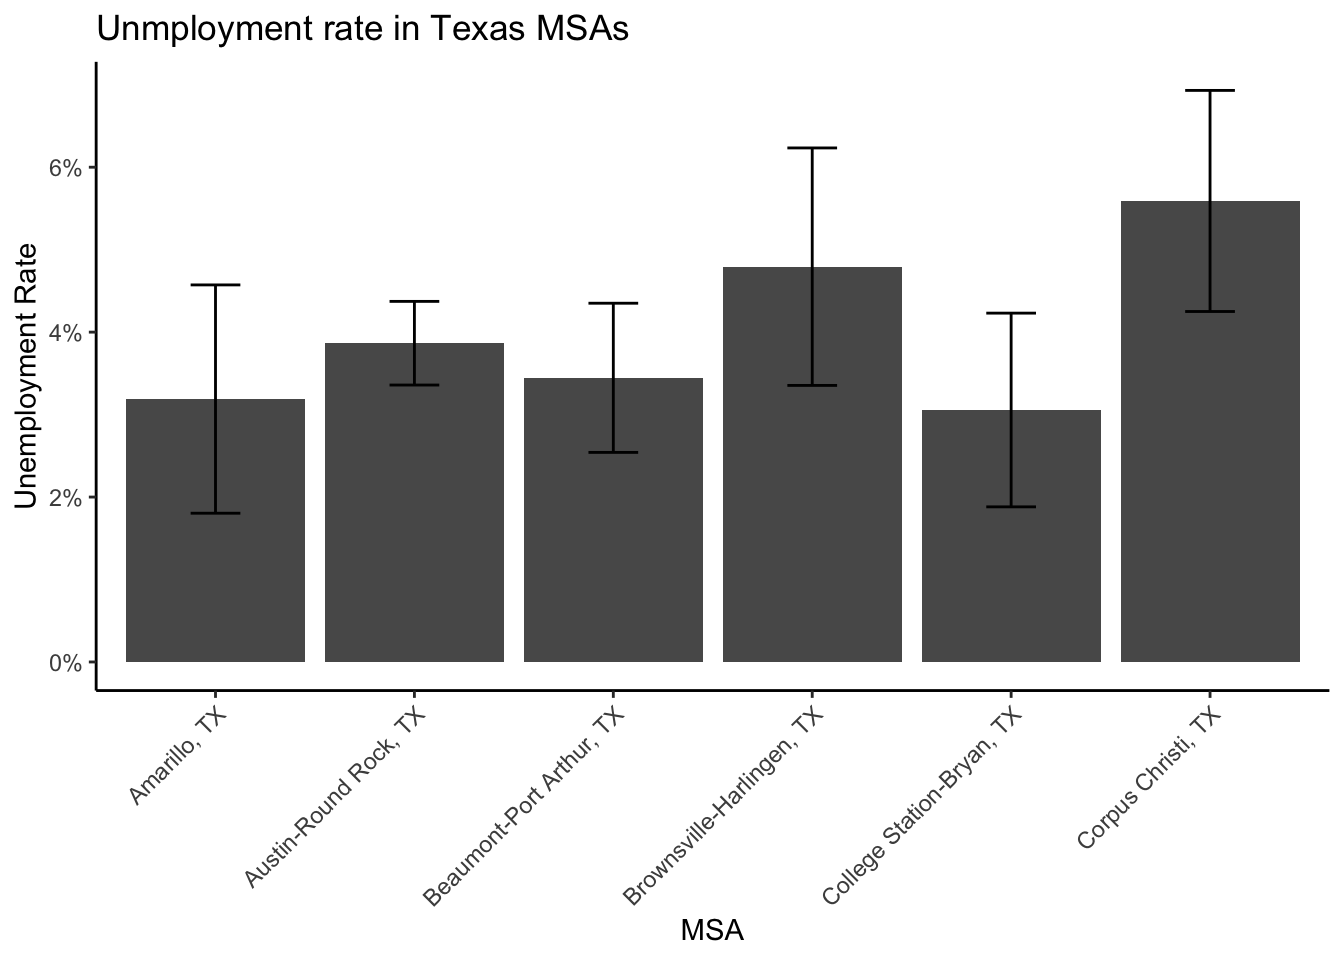
\includegraphics{survey_files/figure-pdf/unnamed-chunk-23-1.pdf}

}

\end{figure}

We see that among the first 6 MSAs in the state (that are in the ACS
microdata), Corpus Christi has the highest unemployment rate a \%, and
College Station-Bryan has the lowest unemployment rate at \%.

We can also use these functions for continuous variables, say with
incomes. In the code below, I pipe all the elements of the analysis
together to illustrate the workflow that we can do to calculate the
median income in each MSA and plot it along with its error.

\begin{Shaded}
\begin{Highlighting}[]
\NormalTok{ipums }\SpecialCharTok{\%\textgreater{}\%}
  \FunctionTok{filter}\NormalTok{(EMPSTAT }\SpecialCharTok{\%in\%} \DecValTok{1}\SpecialCharTok{:}\DecValTok{2}\NormalTok{,}
\NormalTok{         AGE }\SpecialCharTok{\textgreater{}=} \DecValTok{16} \SpecialCharTok{\&}\NormalTok{ AGE }\SpecialCharTok{\textless{}=} \DecValTok{65}\NormalTok{, }
\NormalTok{         MET2013 }\SpecialCharTok{!=} \DecValTok{0}\NormalTok{) }\SpecialCharTok{\%\textgreater{}\%}
  \FunctionTok{mutate}\NormalTok{(}\AttributeTok{income =} \FunctionTok{ifelse}\NormalTok{(INCWAGE }\SpecialCharTok{\textless{}=} \DecValTok{0}\NormalTok{, }\ConstantTok{NA}\NormalTok{, INCWAGE),}
         \AttributeTok{met\_name =}\NormalTok{ haven}\SpecialCharTok{::}\FunctionTok{as\_factor}\NormalTok{(MET2013)) }\SpecialCharTok{\%\textgreater{}\%}
  \FunctionTok{as\_survey\_design}\NormalTok{(}\AttributeTok{cluster =}\NormalTok{ CLUSTER,}
                   \AttributeTok{strata =}\NormalTok{ STRATA,}
                   \AttributeTok{weights =}\NormalTok{ PERWT) }\SpecialCharTok{\%\textgreater{}\%}
  \FunctionTok{group\_by}\NormalTok{(met\_name)}\SpecialCharTok{\%\textgreater{}\%}
  \FunctionTok{summarize}\NormalTok{(}\AttributeTok{median\_wage =} \FunctionTok{survey\_median}\NormalTok{(income, }\AttributeTok{na.rm=}\NormalTok{T)) }\SpecialCharTok{\%\textgreater{}\%}  
  \FunctionTok{head}\NormalTok{() }\SpecialCharTok{\%\textgreater{}\%}
  \FunctionTok{ggplot}\NormalTok{()}\SpecialCharTok{+}
  \FunctionTok{geom\_bar}\NormalTok{(}\FunctionTok{aes}\NormalTok{(}\AttributeTok{x=}\NormalTok{met\_name, }\AttributeTok{y =}\NormalTok{ median\_wage), }\AttributeTok{stat =} \StringTok{"identity"}\NormalTok{)}\SpecialCharTok{+}
  \FunctionTok{geom\_errorbar}\NormalTok{(}\FunctionTok{aes}\NormalTok{(}\AttributeTok{x=}\NormalTok{met\_name,}
                    \AttributeTok{ymin=}\NormalTok{median\_wage}\FloatTok{{-}1.96}\SpecialCharTok{*}\NormalTok{median\_wage\_se,}
                    \AttributeTok{ymax=}\NormalTok{ median\_wage}\FloatTok{+1.96}\SpecialCharTok{*}\NormalTok{median\_wage\_se),}
                \AttributeTok{width=}\NormalTok{.}\DecValTok{25}\NormalTok{)}\SpecialCharTok{+}
  \FunctionTok{scale\_y\_continuous}\NormalTok{(}\AttributeTok{labels =}\NormalTok{ scales}\SpecialCharTok{::}\NormalTok{dollar)}\SpecialCharTok{+}
  \FunctionTok{labs}\NormalTok{(}\AttributeTok{x =} \StringTok{"MSA"}\NormalTok{, }
       \AttributeTok{y =} \StringTok{"Median Wage"}\NormalTok{,}
       \AttributeTok{title =} \StringTok{"Median wage in Texas MSAs"}\NormalTok{)}\SpecialCharTok{+}
  \FunctionTok{theme}\NormalTok{(}\AttributeTok{axis.text.x =} \FunctionTok{element\_text}\NormalTok{(}\AttributeTok{angle =} \DecValTok{45}\NormalTok{, }\AttributeTok{hjust =} \DecValTok{1}\NormalTok{))}
\end{Highlighting}
\end{Shaded}

\begin{figure}[H]

{\centering 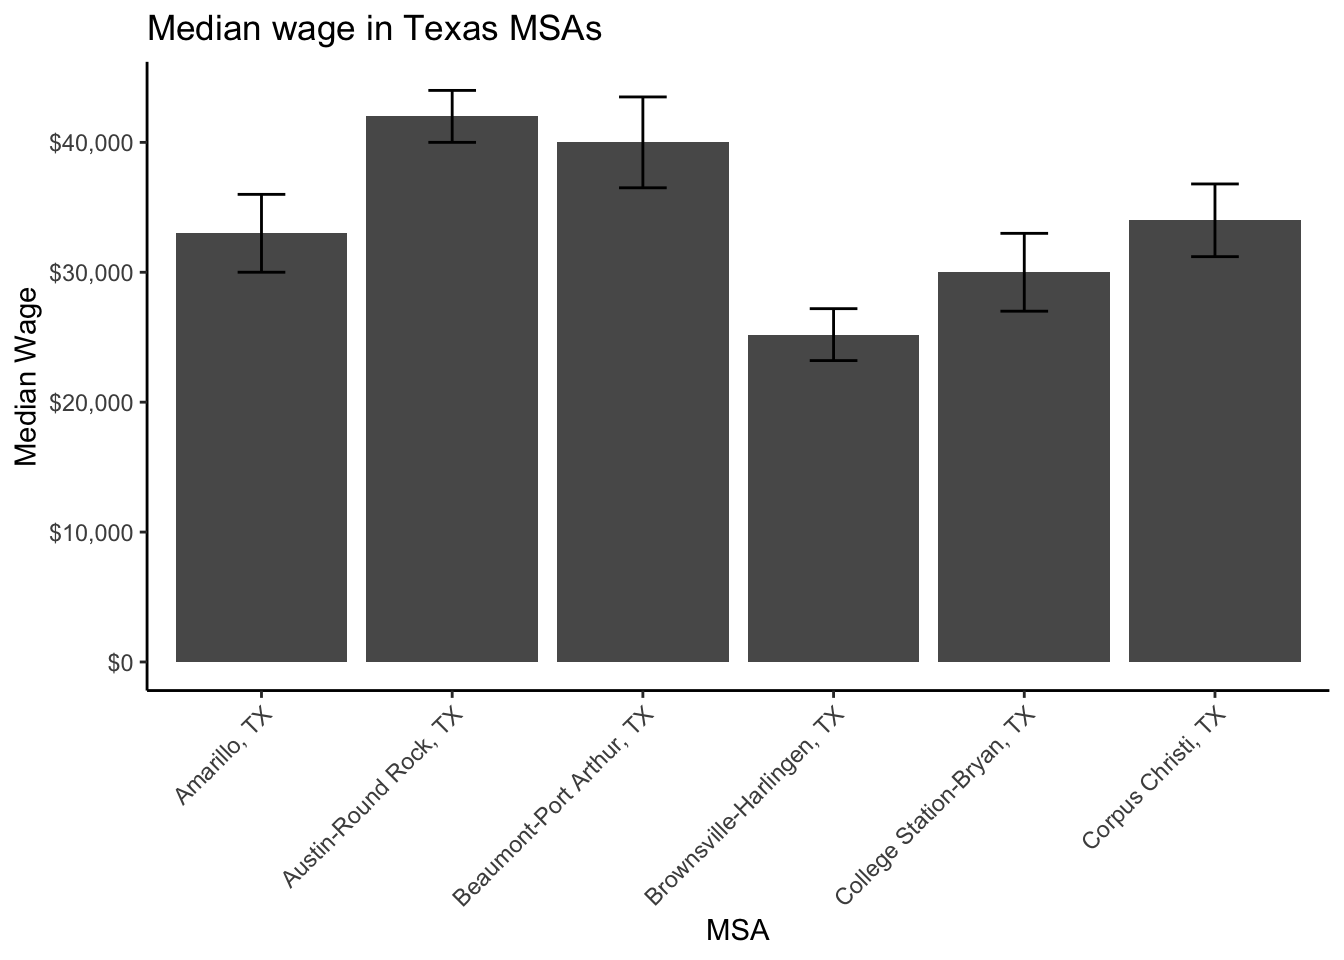
\includegraphics{survey_files/figure-pdf/unnamed-chunk-24-1.pdf}

}

\end{figure}

Which shows that Austin-Round Rock has the highest median wage and
Brownsville-Harlingen has the lowest median wage.

\hypertarget{creating-tables-from-survey-data-analysis}{%
\section{Creating tables from survey data
analysis}\label{creating-tables-from-survey-data-analysis}}

Tabular output from our survey data analysis is possible through several
different means. When using dplyr, our intermediate output of the
analysis is always a data frame, and so any R method for printing data
frames would work for simple tabular display. For instance, if we just
use \texttt{knitr::kable()} on our workflow from above instead of piping
into a plot we would get something like this:

\begin{Shaded}
\begin{Highlighting}[]
\NormalTok{ipums }\SpecialCharTok{\%\textgreater{}\%}
  \FunctionTok{filter}\NormalTok{(EMPSTAT }\SpecialCharTok{\%in\%} \DecValTok{1}\SpecialCharTok{:}\DecValTok{2}\NormalTok{,}
\NormalTok{         AGE }\SpecialCharTok{\textgreater{}=} \DecValTok{16} \SpecialCharTok{\&}\NormalTok{ AGE }\SpecialCharTok{\textless{}=} \DecValTok{65}\NormalTok{, }
\NormalTok{         MET2013 }\SpecialCharTok{!=} \DecValTok{0}\NormalTok{) }\SpecialCharTok{\%\textgreater{}\%}
  \FunctionTok{mutate}\NormalTok{(}\AttributeTok{income =} \FunctionTok{ifelse}\NormalTok{(INCWAGE }\SpecialCharTok{\textless{}=} \DecValTok{0}\NormalTok{, }\ConstantTok{NA}\NormalTok{, INCWAGE),}
         \AttributeTok{met\_name =}\NormalTok{ haven}\SpecialCharTok{::}\FunctionTok{as\_factor}\NormalTok{(MET2013)) }\SpecialCharTok{\%\textgreater{}\%}
  \FunctionTok{as\_survey\_design}\NormalTok{(}\AttributeTok{cluster =}\NormalTok{ CLUSTER,}
                   \AttributeTok{strata =}\NormalTok{ STRATA,}
                   \AttributeTok{weights =}\NormalTok{ PERWT) }\SpecialCharTok{\%\textgreater{}\%}
  \FunctionTok{group\_by}\NormalTok{(met\_name)}\SpecialCharTok{\%\textgreater{}\%}
  \FunctionTok{summarize}\NormalTok{(}\AttributeTok{median\_wage =} \FunctionTok{survey\_median}\NormalTok{(income, }\AttributeTok{na.rm=}\NormalTok{T)) }\SpecialCharTok{\%\textgreater{}\%}  
  \FunctionTok{head}\NormalTok{() }\SpecialCharTok{\%\textgreater{}\%}
\NormalTok{  knitr}\SpecialCharTok{::}\FunctionTok{kable}\NormalTok{(}\AttributeTok{format =} \StringTok{"latex"}\NormalTok{,}
               \AttributeTok{digits =} \DecValTok{0}\NormalTok{,}
               \AttributeTok{caption =} \StringTok{"Median Wages in Texas MSAs"}\NormalTok{,}
               \AttributeTok{align =} \StringTok{\textquotesingle{}c\textquotesingle{}}\NormalTok{,}
               \AttributeTok{col.names =}\FunctionTok{c}\NormalTok{(}\StringTok{"MSA Name"}\NormalTok{, }\StringTok{"Median Wage"}\NormalTok{, }\StringTok{"Median Wage SE"}\NormalTok{))}
\end{Highlighting}
\end{Shaded}

\begin{table}

\caption{Median Wages in Texas MSAs}
\centering
\begin{tabular}[t]{c|c|c}
\hline
MSA Name & Median Wage & Median Wage SE\\
\hline
Amarillo, TX & 33000 & 1529\\
\hline
Austin-Round Rock, TX & 42000 & 1020\\
\hline
Beaumont-Port Arthur, TX & 40000 & 1784\\
\hline
Brownsville-Harlingen, TX & 25200 & 1020\\
\hline
College Station-Bryan, TX & 30000 & 1529\\
\hline
Corpus Christi, TX & 34000 & 1428\\
\hline
\end{tabular}
\end{table}

Which is OK, but there are other ways to make tables for reports. The
\texttt{gt} package (Iannone, Cheng, and Schloerke 2021) is built using
tidyverse principles, and build tables in much the same way that
\texttt{ggplot} builds plots, and fits easily into a dplyr workflow.
Here, I use \texttt{gt} to produce a similar table to that from
\texttt{knitr::kable} from above.

\begin{Shaded}
\begin{Highlighting}[]
\FunctionTok{library}\NormalTok{(gt, }\AttributeTok{quietly =}\NormalTok{ T)}

\NormalTok{ipums }\SpecialCharTok{\%\textgreater{}\%}
  \FunctionTok{filter}\NormalTok{(EMPSTAT }\SpecialCharTok{\%in\%} \DecValTok{1}\SpecialCharTok{:}\DecValTok{2}\NormalTok{,}
\NormalTok{         AGE }\SpecialCharTok{\textgreater{}=} \DecValTok{16} \SpecialCharTok{\&}\NormalTok{ AGE }\SpecialCharTok{\textless{}=} \DecValTok{65}\NormalTok{, }
\NormalTok{         MET2013 }\SpecialCharTok{!=} \DecValTok{0}\NormalTok{) }\SpecialCharTok{\%\textgreater{}\%}
  \FunctionTok{mutate}\NormalTok{(}\AttributeTok{income =} \FunctionTok{ifelse}\NormalTok{(INCWAGE }\SpecialCharTok{\textless{}=} \DecValTok{0}\NormalTok{, }\ConstantTok{NA}\NormalTok{, INCWAGE),}
         \AttributeTok{met\_name =}\NormalTok{ haven}\SpecialCharTok{::}\FunctionTok{as\_factor}\NormalTok{(MET2013)) }\SpecialCharTok{\%\textgreater{}\%}
  \FunctionTok{as\_survey\_design}\NormalTok{(}\AttributeTok{cluster =}\NormalTok{ CLUSTER,}
                   \AttributeTok{strata =}\NormalTok{ STRATA,}
                   \AttributeTok{weights =}\NormalTok{ PERWT) }\SpecialCharTok{\%\textgreater{}\%}
  \FunctionTok{group\_by}\NormalTok{(met\_name)}\SpecialCharTok{\%\textgreater{}\%}
  \FunctionTok{summarize}\NormalTok{(}\AttributeTok{median\_wage =} \FunctionTok{survey\_median}\NormalTok{(income, }\AttributeTok{na.rm=}\NormalTok{T)) }\SpecialCharTok{\%\textgreater{}\%}  
  \FunctionTok{head}\NormalTok{()}\SpecialCharTok{\%\textgreater{}\%}
  \FunctionTok{gt}\NormalTok{() }\SpecialCharTok{\%\textgreater{}\%}
    \FunctionTok{tab\_header}\NormalTok{(}\AttributeTok{title =} \StringTok{"Median Wages in Texas MSAs"}\NormalTok{)}\SpecialCharTok{\%\textgreater{}\%}
    \FunctionTok{cols\_label}\NormalTok{(}\AttributeTok{met\_name =} \StringTok{"MSA Name"}\NormalTok{,}
                 \AttributeTok{median\_wage =} \StringTok{"Median Wage"}\NormalTok{,}
                 \AttributeTok{median\_wage\_se =} \StringTok{"Median Wage SE"}\NormalTok{)}\SpecialCharTok{\%\textgreater{}\%}
    \FunctionTok{fmt\_number}\NormalTok{(}\AttributeTok{columns =} \FunctionTok{c}\NormalTok{( median\_wage,  median\_wage\_se), }
                 \AttributeTok{decimals =} \DecValTok{0}\NormalTok{, }\AttributeTok{use\_seps =} \ConstantTok{TRUE}\NormalTok{)}
\end{Highlighting}
\end{Shaded}

\begin{longtable*}{crr}
\caption*{
{\large Median Wages in Texas MSAs}
} \\ 
\toprule
MSA Name & Median Wage & Median Wage SE \\ 
\midrule
Amarillo, TX & $33,000$ & $1,529$ \\ 
Austin-Round Rock, TX & $42,000$ & $1,020$ \\ 
Beaumont-Port Arthur, TX & $40,000$ & $1,784$ \\ 
Brownsville-Harlingen, TX & $25,200$ & $1,020$ \\ 
College Station-Bryan, TX & $30,000$ & $1,529$ \\ 
Corpus Christi, TX & $34,000$ & $1,428$ \\ 
\bottomrule
\end{longtable*}

In general, the \texttt{gt} tables are much easier to make look nice,
compared to basic tables, because they're much more customizable. The
\texttt{gtsummary} package extends the table functionality by combining
the summary functions like \texttt{dplyr} with the table structures of
\texttt{gt}. Additionally, it will recognize survey design objects so
that information can also be integrated into your workflow. The
\texttt{gtsummary} presents a more descriptive statistical summary of
the variables included, and actually uses \texttt{dplyr} tools under the
hood of the package.

In the code below, I first filter and mutate the IPUMS data to contain
working age people who are employed, and who live in the six Texas
cities featured in the examples above. I also create a new income
variable that excludes all zero incomes, and drop levels of the
\texttt{MET2013} variable that aren't in the list I specified. This
pipes into the survey design function from the \texttt{survey} package,
which pipes into the \texttt{tbl\_svysummary} function which summarizes
income for each MSA. This function has a lot of options to specify its
output, and I recommend you consult the examples at the author's
website\footnote{http://www.danieldsjoberg.com/gtsummary/}.

\begin{Shaded}
\begin{Highlighting}[]
\FunctionTok{library}\NormalTok{(gtsummary)}

\NormalTok{ipums }\SpecialCharTok{\%\textgreater{}\%}
 \FunctionTok{filter}\NormalTok{(EMPSTAT }\SpecialCharTok{==} \DecValTok{1}\NormalTok{,}
\NormalTok{         AGE }\SpecialCharTok{\textgreater{}=} \DecValTok{16} \SpecialCharTok{\&}\NormalTok{ AGE }\SpecialCharTok{\textless{}=} \DecValTok{65}\NormalTok{, }
\NormalTok{         MET2013 }\SpecialCharTok{!=} \DecValTok{0}\NormalTok{, }
\NormalTok{         MET2013 }\SpecialCharTok{\%in\%} \FunctionTok{c}\NormalTok{(}\DecValTok{11100}\NormalTok{, }\DecValTok{12420}\NormalTok{, }\DecValTok{13140}\NormalTok{, }\DecValTok{15180}\NormalTok{, }\DecValTok{17780}\NormalTok{, }\DecValTok{18580}\NormalTok{)) }\SpecialCharTok{\%\textgreater{}\%} 
  \FunctionTok{mutate}\NormalTok{(}\AttributeTok{income =} \FunctionTok{ifelse}\NormalTok{(INCWAGE }\SpecialCharTok{\textless{}=} \DecValTok{0}\NormalTok{, }\ConstantTok{NA}\NormalTok{, INCWAGE),}
         \AttributeTok{met\_name =}\NormalTok{ haven}\SpecialCharTok{::}\FunctionTok{as\_factor}\NormalTok{(MET2013))}\SpecialCharTok{\%\textgreater{}\%}
  \FunctionTok{select}\NormalTok{(met\_name,  income, CLUSTER, STRATA, PERWT)}\SpecialCharTok{\%\textgreater{}\%}
  \FunctionTok{droplevels}\NormalTok{()}\SpecialCharTok{\%\textgreater{}\%}
\NormalTok{  survey}\SpecialCharTok{::}\FunctionTok{svydesign}\NormalTok{(}\AttributeTok{id =} \SpecialCharTok{\textasciitilde{}}\NormalTok{ CLUSTER,}
                   \AttributeTok{strata =} \SpecialCharTok{\textasciitilde{}}\NormalTok{ STRATA,}
                   \AttributeTok{weights =} \SpecialCharTok{\textasciitilde{}}\NormalTok{ PERWT,}
                \AttributeTok{data =}\NormalTok{ .) }\SpecialCharTok{\%\textgreater{}\%}
   \FunctionTok{tbl\_svysummary}\NormalTok{(}\AttributeTok{by =} \StringTok{"met\_name"}\NormalTok{,}
                  \AttributeTok{missing =} \StringTok{"no"}\NormalTok{,}
                  \AttributeTok{include =} \FunctionTok{c}\NormalTok{(met\_name, income), }
                  \AttributeTok{label =} \FunctionTok{list}\NormalTok{(}\AttributeTok{income =} \StringTok{"Median Wage"}\NormalTok{))}\SpecialCharTok{\%\textgreater{}\%}
  \FunctionTok{as\_hux\_table}\NormalTok{()}
\end{Highlighting}
\end{Shaded}

 
  \providecommand{\huxb}[2]{\arrayrulecolor[RGB]{#1}\global\arrayrulewidth=#2pt}
  \providecommand{\huxvb}[2]{\color[RGB]{#1}\vrule width #2pt}
  \providecommand{\huxtpad}[1]{\rule{0pt}{#1}}
  \providecommand{\huxbpad}[1]{\rule[-#1]{0pt}{#1}}

\begin{table}[ht]
\begin{centerbox}
\begin{threeparttable}
 
\setlength{\tabcolsep}{0pt}
\begin{tabular}{l l l l l l l}


\hhline{}
\arrayrulecolor{black}

\multicolumn{1}{!{\huxvb{0, 0, 0}{0}}l!{\huxvb{0, 0, 0}{0}}}{\huxtpad{6pt + 1em}\raggedright \hspace{6pt} \textbf{Characteristic}
 \hspace{6pt}\huxbpad{6pt}} &
\multicolumn{1}{c!{\huxvb{0, 0, 0}{0}}}{\huxtpad{6pt + 1em}\centering \hspace{6pt} \textbf{Amarillo, TX}, N = 114,201
 \hspace{6pt}\huxbpad{6pt}} &
\multicolumn{1}{c!{\huxvb{0, 0, 0}{0}}}{\huxtpad{6pt + 1em}\centering \hspace{6pt} \textbf{Austin-Round Rock, TX}, N = 1,193,654
 \hspace{6pt}\huxbpad{6pt}} &
\multicolumn{1}{c!{\huxvb{0, 0, 0}{0}}}{\huxtpad{6pt + 1em}\centering \hspace{6pt} \textbf{Beaumont-Port Arthur, TX}, N = 163,936
 \hspace{6pt}\huxbpad{6pt}} &
\multicolumn{1}{c!{\huxvb{0, 0, 0}{0}}}{\huxtpad{6pt + 1em}\centering \hspace{6pt} \textbf{Brownsville-Harlingen, TX}, N = 161,922
 \hspace{6pt}\huxbpad{6pt}} &
\multicolumn{1}{c!{\huxvb{0, 0, 0}{0}}}{\huxtpad{6pt + 1em}\centering \hspace{6pt} \textbf{College Station-Bryan, TX}, N = 111,576
 \hspace{6pt}\huxbpad{6pt}} &
\multicolumn{1}{c!{\huxvb{0, 0, 0}{0}}}{\huxtpad{6pt + 1em}\centering \hspace{6pt} \textbf{Corpus Christi, TX}, N = 208,801
 \hspace{6pt}\huxbpad{6pt}} \tabularnewline[-0.5pt]


\hhline{>{\huxb{0, 0, 0}{0.4}}->{\huxb{0, 0, 0}{0.4}}->{\huxb{0, 0, 0}{0.4}}->{\huxb{0, 0, 0}{0.4}}->{\huxb{0, 0, 0}{0.4}}->{\huxb{0, 0, 0}{0.4}}->{\huxb{0, 0, 0}{0.4}}-}
\arrayrulecolor{black}

\multicolumn{1}{!{\huxvb{0, 0, 0}{0}}l!{\huxvb{0, 0, 0}{0}}}{\huxtpad{6pt + 1em}\raggedright \hspace{6pt} Median Wage \hspace{6pt}\huxbpad{6pt}} &
\multicolumn{1}{c!{\huxvb{0, 0, 0}{0}}}{\huxtpad{6pt + 1em}\centering \hspace{6pt} 34,000 (19,200, 56,000) \hspace{6pt}\huxbpad{6pt}} &
\multicolumn{1}{c!{\huxvb{0, 0, 0}{0}}}{\huxtpad{6pt + 1em}\centering \hspace{6pt} 43,000 (24,000, 75,000) \hspace{6pt}\huxbpad{6pt}} &
\multicolumn{1}{c!{\huxvb{0, 0, 0}{0}}}{\huxtpad{6pt + 1em}\centering \hspace{6pt} 40,000 (20,000, 67,000) \hspace{6pt}\huxbpad{6pt}} &
\multicolumn{1}{c!{\huxvb{0, 0, 0}{0}}}{\huxtpad{6pt + 1em}\centering \hspace{6pt} 26,000 (14,000, 47,000) \hspace{6pt}\huxbpad{6pt}} &
\multicolumn{1}{c!{\huxvb{0, 0, 0}{0}}}{\huxtpad{6pt + 1em}\centering \hspace{6pt} 30,000 (14,000, 51,111) \hspace{6pt}\huxbpad{6pt}} &
\multicolumn{1}{c!{\huxvb{0, 0, 0}{0}}}{\huxtpad{6pt + 1em}\centering \hspace{6pt} 35,000 (20,000, 58,000) \hspace{6pt}\huxbpad{6pt}} \tabularnewline[-0.5pt]


\hhline{>{\huxb{0, 0, 0}{0.8}}->{\huxb{0, 0, 0}{0.8}}->{\huxb{0, 0, 0}{0.8}}->{\huxb{0, 0, 0}{0.8}}->{\huxb{0, 0, 0}{0.8}}->{\huxb{0, 0, 0}{0.8}}->{\huxb{0, 0, 0}{0.8}}-}
\arrayrulecolor{black}

\multicolumn{7}{!{\huxvb{0, 0, 0}{0}}l!{\huxvb{0, 0, 0}{0}}}{\huxtpad{6pt + 1em}\raggedright \hspace{6pt} Median (IQR) \hspace{6pt}\huxbpad{6pt}} \tabularnewline[-0.5pt]


\hhline{}
\arrayrulecolor{black}
\end{tabular}
\end{threeparttable}\par\end{centerbox}

\end{table}
 

\hypertarget{how-this-differs-from-simple-random-sampling}{%
\subsection{How this differs from simple random
sampling}\label{how-this-differs-from-simple-random-sampling}}

So the big question I often get from students is ``Do I really need to
weight my analysis?'' and of course, I say, ``Of course!''. Weights
don't just inflate your data to the population, they serve a very
important role in making sure your sample data aren't biased in their
scope. Bias can enter into survey data in many forms, but nonresponse
bias can dramatically affect population based estimates if key segments
of our target population respond at low rates. Surveys will often deal
with this by rigorous data collection strategies, but often the survey
designers have to account for the added probability of nonresponse by
modification of their basic weights. Lohr (2019) describes how this is
done using a variety of methods including raking and post
stratification, which typically separate the sample into subdivisions
based on one or more demographic characteristic and produce weights
based on how the sample deviates from the population composition. These
methods are robust and are commonly used in large national surveys
including the Behavioral Risk Factor Surveillance system (BRFSS).

Other reasons for weighting and why it matters are oversampling. Many
surveys will do this in their data collection because an important
element of their target population may be small in overall size, so they
will sample more respondents from that population subgroup than their
proportion in the larger population would predict. For example, if a
survey wanted to get detailed data on recent refugees to a country, and
this group is small, say .1 percent of the overall population, they may
design their study to have 10\% of their survey respondents be refugees.
This oversampling can be accounted for in the survey weights so the
additional respondents are down-weighted to represent their fraction of
the target population, while still allowing the researchers to get a
large sample from this group. Surveys such as the Early Childhood
Longitudinal Surveys and the National Longitudinal Study of Adolescent
to Adult Health (AddHealth) routinely over-sample specific groups. For
example the AddHealth over-samples black adolescents with college
educated parents, Cuban, Puerto Rican, Chinese, and physically disabled
adolescents.

\hypertarget{how-do-weights-affect-our-estimates}{%
\subsection{How do weights affect our
estimates?}\label{how-do-weights-affect-our-estimates}}

In the code example below, I illustrate how not including sample weights
affects the estimates generated. This in effect is how traditional
statistical analysis assuming random sampling would do things. So in
order to compare the weighted estimates to the unweighted estimates, all
we need to do is use a non-survey design oriented method to produce our
estimate, and compare it to the survey design oriented method. Note that
many surveys are designed to be \emph{self-weighting}, so weights are
not provided nor necessary, again, read the documentation for your
specific survey for what it recommends.

\begin{Shaded}
\begin{Highlighting}[]
\NormalTok{srs}\OtherTok{\textless{}{-}}\NormalTok{ipums }\SpecialCharTok{\%\textgreater{}\%}
  \FunctionTok{filter}\NormalTok{(EMPSTAT }\SpecialCharTok{\%in\%} \DecValTok{1}\SpecialCharTok{:}\DecValTok{2}\NormalTok{,}
\NormalTok{         AGE }\SpecialCharTok{\textgreater{}=} \DecValTok{16} \SpecialCharTok{\&}\NormalTok{ AGE }\SpecialCharTok{\textless{}=} \DecValTok{65}\NormalTok{, }
\NormalTok{         MET2013 }\SpecialCharTok{!=} \DecValTok{0}\NormalTok{) }\SpecialCharTok{\%\textgreater{}\%}
  \FunctionTok{mutate}\NormalTok{(}\AttributeTok{employed =} \FunctionTok{as.factor}\NormalTok{(}\FunctionTok{case\_when}\NormalTok{(.}\SpecialCharTok{$}\NormalTok{EMPSTAT }\SpecialCharTok{==} \DecValTok{1} \SpecialCharTok{\textasciitilde{}} \StringTok{"Employed"}\NormalTok{,}
\NormalTok{                              .}\SpecialCharTok{$}\NormalTok{EMPSTAT }\SpecialCharTok{==} \DecValTok{2} \SpecialCharTok{\textasciitilde{}} \StringTok{"Unemployed"}\NormalTok{ )),}
         \AttributeTok{met\_name =}\NormalTok{ haven}\SpecialCharTok{::}\FunctionTok{as\_factor}\NormalTok{(MET2013)) }\SpecialCharTok{\%\textgreater{}\%}
  \FunctionTok{group\_by}\NormalTok{(met\_name)}\SpecialCharTok{\%\textgreater{}\%}
  \FunctionTok{summarize}\NormalTok{(}\AttributeTok{emp\_rate =} \FunctionTok{mean}\NormalTok{(}\FunctionTok{I}\NormalTok{(employed)}\SpecialCharTok{==}\StringTok{"Employed"}\NormalTok{),}
            \AttributeTok{emp\_rate\_se =} \FunctionTok{sd}\NormalTok{(}\FunctionTok{I}\NormalTok{(employed)}\SpecialCharTok{==}\StringTok{"Employed"}\NormalTok{)}\SpecialCharTok{/}\FunctionTok{sqrt}\NormalTok{(}\FunctionTok{n}\NormalTok{()))}\SpecialCharTok{\%\textgreater{}\%}
   \CommentTok{\# pivot\_wider(id = met\_name,}
   \CommentTok{\#            names\_from = employed,}
   \CommentTok{\#            values\_from = c(emp\_rate, emp\_rate\_se) ) \%\textgreater{}\%}
  \FunctionTok{head}\NormalTok{()}
\NormalTok{srs}\SpecialCharTok{$}\NormalTok{estimate}\OtherTok{\textless{}{-}}\StringTok{"Unweighted"}
\end{Highlighting}
\end{Shaded}

\begin{Shaded}
\begin{Highlighting}[]
\NormalTok{surv.est}\OtherTok{\textless{}{-}}\NormalTok{ipums }\SpecialCharTok{\%\textgreater{}\%}
  \FunctionTok{filter}\NormalTok{(EMPSTAT }\SpecialCharTok{\%in\%} \DecValTok{1}\SpecialCharTok{:}\DecValTok{2}\NormalTok{,}
\NormalTok{         AGE }\SpecialCharTok{\textgreater{}=} \DecValTok{16} \SpecialCharTok{\&}\NormalTok{ AGE }\SpecialCharTok{\textless{}=} \DecValTok{65}\NormalTok{, }
\NormalTok{         MET2013 }\SpecialCharTok{!=} \DecValTok{0}\NormalTok{) }\SpecialCharTok{\%\textgreater{}\%}
  \FunctionTok{mutate}\NormalTok{(}\AttributeTok{employed =} \FunctionTok{as.factor}\NormalTok{(}\FunctionTok{case\_when}\NormalTok{(.}\SpecialCharTok{$}\NormalTok{EMPSTAT }\SpecialCharTok{==} \DecValTok{1} \SpecialCharTok{\textasciitilde{}} \StringTok{"Employed"}\NormalTok{,}
\NormalTok{                              .}\SpecialCharTok{$}\NormalTok{EMPSTAT }\SpecialCharTok{==} \DecValTok{2} \SpecialCharTok{\textasciitilde{}} \StringTok{"Unemployed"}\NormalTok{ )),}
         \AttributeTok{met\_name =}\NormalTok{ haven}\SpecialCharTok{::}\FunctionTok{as\_factor}\NormalTok{(MET2013)) }\SpecialCharTok{\%\textgreater{}\%}
  \FunctionTok{as\_survey\_design}\NormalTok{(}\AttributeTok{cluster =}\NormalTok{ CLUSTER,}
                   \AttributeTok{strata =}\NormalTok{ STRATA,}
                   \AttributeTok{weights =}\NormalTok{ PERWT) }\SpecialCharTok{\%\textgreater{}\%}
  \FunctionTok{group\_by}\NormalTok{(met\_name)}\SpecialCharTok{\%\textgreater{}\%}
  \FunctionTok{summarize}\NormalTok{(}\AttributeTok{emp\_rate =} \FunctionTok{survey\_mean}\NormalTok{(}\FunctionTok{I}\NormalTok{(employed)}\SpecialCharTok{==}\StringTok{"Employed"}\NormalTok{)) }\SpecialCharTok{\%\textgreater{}\%}  
  \CommentTok{\#rename(emp\_rate\_surv = emp\_rate, emp\_rate\_se\_surv = emp\_rate\_se)\%\textgreater{}\%}
  \FunctionTok{head}\NormalTok{()}

\NormalTok{surv.est}\SpecialCharTok{$}\NormalTok{estimate}\OtherTok{\textless{}{-}}\StringTok{"Weighted"}
\end{Highlighting}
\end{Shaded}

\begin{Shaded}
\begin{Highlighting}[]
\NormalTok{merged }\OtherTok{\textless{}{-}} \FunctionTok{rbind}\NormalTok{(srs, surv.est)}
\NormalTok{p1}\OtherTok{\textless{}{-}}\NormalTok{merged}\SpecialCharTok{\%\textgreater{}\%}
  \FunctionTok{ggplot}\NormalTok{(}\FunctionTok{aes}\NormalTok{(}\AttributeTok{y =}\NormalTok{ emp\_rate, }\AttributeTok{x =}\NormalTok{ met\_name , }\AttributeTok{color =}\NormalTok{ estimate))}\SpecialCharTok{+}
  \FunctionTok{geom\_point}\NormalTok{(}\AttributeTok{stat=}\StringTok{"identity"}\NormalTok{,}
             \AttributeTok{cex=}\DecValTok{2}\NormalTok{)}\SpecialCharTok{+}
  \FunctionTok{geom\_line}\NormalTok{(}\FunctionTok{aes}\NormalTok{(}\AttributeTok{group =}\NormalTok{ met\_name),}
            \AttributeTok{col =} \StringTok{"grey"}\NormalTok{)}\SpecialCharTok{+}
  \FunctionTok{scale\_y\_continuous}\NormalTok{(}\AttributeTok{labels =}\NormalTok{ scales}\SpecialCharTok{::}\NormalTok{percent)}\SpecialCharTok{+}
  \FunctionTok{scale\_color\_discrete}\NormalTok{( }\AttributeTok{name =} \StringTok{"Estimate Type"}\NormalTok{)}\SpecialCharTok{\%\textgreater{}\%}
  \FunctionTok{labs}\NormalTok{(}\AttributeTok{x =} \StringTok{"MSA"}\NormalTok{, }
       \AttributeTok{y =} \StringTok{"Employment Rate Estimate"}\NormalTok{,}
       \AttributeTok{title =} \StringTok{"Employment rate in Texas MSAs"}\NormalTok{,}
       \AttributeTok{subtitle =} \StringTok{"Rate estimates"}\NormalTok{)}\SpecialCharTok{+}
  \FunctionTok{theme}\NormalTok{(}\AttributeTok{axis.text.x =} \FunctionTok{element\_text}\NormalTok{(}\AttributeTok{angle =} \DecValTok{45}\NormalTok{, }\AttributeTok{hjust =} \DecValTok{1}\NormalTok{))}

\NormalTok{p2}\OtherTok{\textless{}{-}}\NormalTok{merged}\SpecialCharTok{\%\textgreater{}\%}
  \FunctionTok{ggplot}\NormalTok{(}\FunctionTok{aes}\NormalTok{(}\AttributeTok{y =}\NormalTok{ emp\_rate\_se, }\AttributeTok{x =}\NormalTok{ met\_name , }\AttributeTok{color =}\NormalTok{ estimate))}\SpecialCharTok{+}
  \FunctionTok{geom\_point}\NormalTok{(}\AttributeTok{stat=}\StringTok{"identity"}\NormalTok{,}
             \AttributeTok{cex=}\DecValTok{2}\NormalTok{)}\SpecialCharTok{+}
  \FunctionTok{geom\_line}\NormalTok{(}\FunctionTok{aes}\NormalTok{(}\AttributeTok{group =}\NormalTok{ met\_name),}
            \AttributeTok{col =} \StringTok{"grey"}\NormalTok{)}\SpecialCharTok{+}
  \FunctionTok{scale\_color\_discrete}\NormalTok{()}\SpecialCharTok{\%\textgreater{}\%}
  \FunctionTok{labs}\NormalTok{(}\AttributeTok{x =} \StringTok{"MSA"}\NormalTok{, }
       \AttributeTok{y =} \StringTok{"Standard Error"}\NormalTok{,}
       \AttributeTok{title =} \StringTok{""}\NormalTok{,}
       \AttributeTok{subtitle =} \StringTok{"Standard error of estimates"}\NormalTok{)}\SpecialCharTok{+}
  \FunctionTok{theme}\NormalTok{(}\AttributeTok{axis.text.x =} \FunctionTok{element\_text}\NormalTok{(}\AttributeTok{angle =} \DecValTok{45}\NormalTok{, }\AttributeTok{hjust =} \DecValTok{1}\NormalTok{))}

\FunctionTok{library}\NormalTok{(patchwork)}

\NormalTok{(p1 }\SpecialCharTok{+}\NormalTok{ p2)}
\end{Highlighting}
\end{Shaded}

\begin{figure}[H]

{\centering 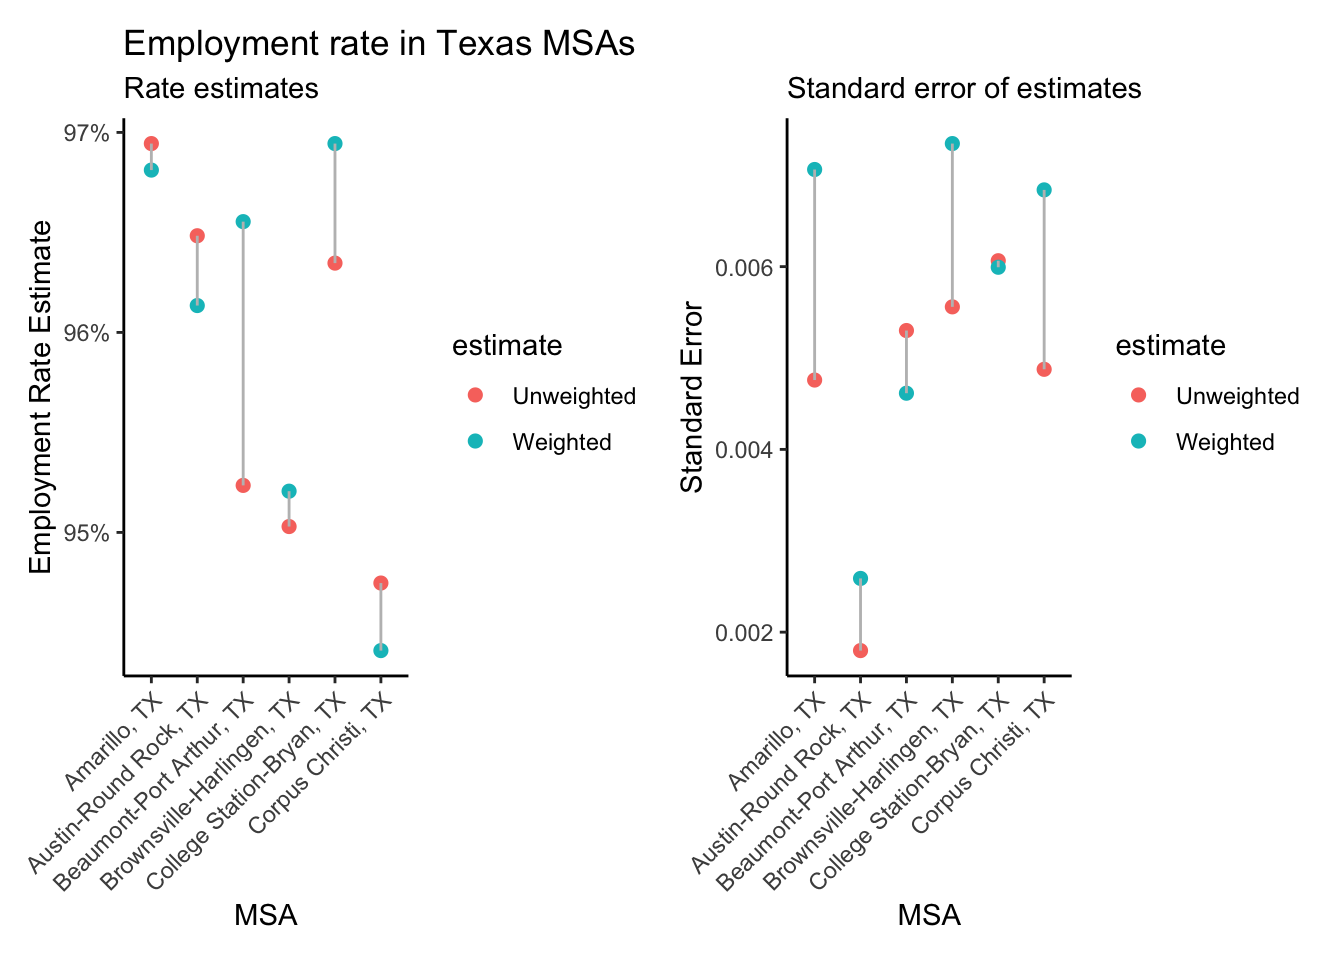
\includegraphics{survey_files/figure-pdf/unnamed-chunk-30-1.pdf}

}

\end{figure}

We see that the difference in the weighted and unweighted estimates do
vary by MSA, as do the standard errors of the estimates, with the
survey-design calculated standard errors nearly always being higher than
those assuming simple random sampling. If our data came from a survey
with more extreme oversampling we would likely see larger differences in
these estimates, and it is generally advisable to include both weights
and survey design elements in all analysis of complex survey data.

\hypertarget{basic-statistical-testing-on-survey-data.}{%
\section{Basic statistical testing on survey
data.}\label{basic-statistical-testing-on-survey-data.}}

To perform basic bivariate statistical tests for frequency tables, the
\texttt{srvyr::svychisq} and \texttt{survey::svy\_chisq} are the primary
tools you need. These will test for basic independence among rows and
columns of a frequency table. Below is an example on how you would test
for independence of labor force participation and gender in the IPUMS
ACS data.

\begin{Shaded}
\begin{Highlighting}[]
\NormalTok{ipums }\SpecialCharTok{\%\textgreater{}\%}
  \FunctionTok{filter}\NormalTok{(EMPSTAT }\SpecialCharTok{!=} \DecValTok{0}\NormalTok{,}
\NormalTok{         AGE }\SpecialCharTok{\textgreater{}=} \DecValTok{16} \SpecialCharTok{\&}\NormalTok{ AGE }\SpecialCharTok{\textless{}=} \DecValTok{65}\NormalTok{) }\SpecialCharTok{\%\textgreater{}\%}
  \FunctionTok{mutate}\NormalTok{(}\AttributeTok{lab\_force\_part =} \FunctionTok{ifelse}\NormalTok{ (}\AttributeTok{test =}\NormalTok{ EMPSTAT }\SpecialCharTok{\%in\%} \FunctionTok{c}\NormalTok{(}\DecValTok{1}\NormalTok{,}\DecValTok{2}\NormalTok{),}
                                  \AttributeTok{yes =} \DecValTok{1}\NormalTok{,}
                                  \AttributeTok{no =} \DecValTok{0}\NormalTok{), }
         \AttributeTok{gender =} \FunctionTok{ifelse}\NormalTok{(}\AttributeTok{test =}\NormalTok{ SEX }\SpecialCharTok{==}\DecValTok{1}\NormalTok{,}
                         \AttributeTok{yes =} \StringTok{"Male"}\NormalTok{,}
                         \AttributeTok{no =} \StringTok{"Female"}\NormalTok{)) }\SpecialCharTok{\%\textgreater{}\%}
  \FunctionTok{as\_survey\_design}\NormalTok{(}\AttributeTok{cluster =}\NormalTok{ CLUSTER,}
                   \AttributeTok{strata =}\NormalTok{ STRATA,}
                   \AttributeTok{weights =}\NormalTok{ PERWT) }\SpecialCharTok{\%\textgreater{}\%}
  \FunctionTok{svychisq}\NormalTok{(}\SpecialCharTok{\textasciitilde{}}\NormalTok{lab\_force\_part}\SpecialCharTok{+}\NormalTok{gender,}
                    \AttributeTok{design =}\NormalTok{ .)}
\end{Highlighting}
\end{Shaded}

\begin{verbatim}

    Pearson's X^2: Rao & Scott adjustment

data:  NextMethod()
F = 1955.4, ndf = 1, ddf = 172976, p-value < 0.00000000000000022
\end{verbatim}

The output above is for the survey adjusted chi square test (Rao and
Scott 1984), which is actually calculated as an F-test in this case. We
see a large F-test value, and a very small p value, which indicates that
men and women have different labor force participation rates. Using our
workflow from above, we can calculate the actual rates as well.

\begin{Shaded}
\begin{Highlighting}[]
\NormalTok{ipums }\SpecialCharTok{\%\textgreater{}\%}
  \FunctionTok{filter}\NormalTok{(EMPSTAT }\SpecialCharTok{!=} \DecValTok{0}\NormalTok{,}
\NormalTok{         AGE }\SpecialCharTok{\textgreater{}=} \DecValTok{16} \SpecialCharTok{\&}\NormalTok{ AGE }\SpecialCharTok{\textless{}=} \DecValTok{65}\NormalTok{) }\SpecialCharTok{\%\textgreater{}\%}
  \FunctionTok{mutate}\NormalTok{(}\AttributeTok{lab\_force\_part =} \FunctionTok{ifelse}\NormalTok{ (}\AttributeTok{test =}\NormalTok{ EMPSTAT }\SpecialCharTok{\%in\%} \FunctionTok{c}\NormalTok{(}\DecValTok{1}\NormalTok{,}\DecValTok{2}\NormalTok{),}
                                  \AttributeTok{yes =} \DecValTok{1}\NormalTok{,}
                                  \AttributeTok{no =} \DecValTok{0}\NormalTok{), }
         \AttributeTok{gender =} \FunctionTok{ifelse}\NormalTok{(}\AttributeTok{test =}\NormalTok{ SEX }\SpecialCharTok{==}\DecValTok{1}\NormalTok{,}
                         \AttributeTok{yes =} \StringTok{"Male"}\NormalTok{,}
                         \AttributeTok{no =} \StringTok{"Female"}\NormalTok{)) }\SpecialCharTok{\%\textgreater{}\%}
  \FunctionTok{as\_survey\_design}\NormalTok{(}\AttributeTok{cluster =}\NormalTok{ CLUSTER,}
                   \AttributeTok{strata =}\NormalTok{ STRATA,}
                   \AttributeTok{weights =}\NormalTok{ PERWT) }\SpecialCharTok{\%\textgreater{}\%}
  \FunctionTok{group\_by}\NormalTok{(gender)}\SpecialCharTok{\%\textgreater{}\%}
  \FunctionTok{summarize}\NormalTok{(}\AttributeTok{lf\_part\_rate =} \FunctionTok{survey\_mean}\NormalTok{(lab\_force\_part, }\AttributeTok{na.rm=}\NormalTok{T)) }\SpecialCharTok{\%\textgreater{}\%}  
  \FunctionTok{head}\NormalTok{()}\SpecialCharTok{\%\textgreater{}\%}
  \FunctionTok{gt}\NormalTok{() }\SpecialCharTok{\%\textgreater{}\%}
    \FunctionTok{tab\_header}\NormalTok{(}\AttributeTok{title =} \StringTok{"Labor Force Participation Rates in Texas"}\NormalTok{)}\SpecialCharTok{\%\textgreater{}\%}
    \FunctionTok{cols\_label}\NormalTok{(}\AttributeTok{gender =} \StringTok{"Gender"}\NormalTok{,}
                 \AttributeTok{lf\_part\_rate =} \StringTok{"Labor Force Participation Rate"}\NormalTok{,}
                \AttributeTok{lf\_part\_rate\_se =} \StringTok{"SE"}\NormalTok{)}\SpecialCharTok{\%\textgreater{}\%}
    \FunctionTok{fmt\_number}\NormalTok{(}\AttributeTok{columns =} \FunctionTok{c}\NormalTok{( lf\_part\_rate,  lf\_part\_rate\_se), }
                 \AttributeTok{decimals =} \DecValTok{3}\NormalTok{, }\AttributeTok{use\_seps =} \ConstantTok{TRUE}\NormalTok{)}
\end{Highlighting}
\end{Shaded}

\begin{longtable*}{lrr}
\caption*{
{\large Labor Force Participation Rates in Texas}
} \\ 
\toprule
Gender & Labor Force Participation Rate & SE \\ 
\midrule
Female & $0.674$ & $0.002$ \\ 
Male & $0.797$ & $0.002$ \\ 
\bottomrule
\end{longtable*}

So we see that males have a much higher labor force participation rate,
compared to females, and this puts the differences that we observed from
the chi square test into better context.

\hypertarget{regression-and-survey-design}{%
\subsection{Regression and survey
design}\label{regression-and-survey-design}}

The design of our surveys affect the most basic estimates we do, and
likewise, the design affects the more complicated analysis as well.
Regression models are the work horse of social science research and we
will spend a significant amount of the chapters that follow on thorough
inspection of them. In the context of this chapter, I felt like I need
to show both how to include survey design in a regression model and
illustrate that weighting and survey design matters in terms of the
output from out models. This section is \emph{NOT} a total coverage of
these models, and is at best a short example. This example will go in a
different direction and use data from the Demographic and Health Survey
instead of the ACS.

The Demographic and Health Survey (DHS) data have been collected since
the mid 1980's in over 90 countries around the world, and the DHS
provides a public model data set that represents data on real
households, without a specific national context. These data are provided
to let people learn how to use the data before applying for access. The
model data can be downloaded freely from the DHS{[}\^{}surveydata-3{]}
as a SAS or STATA format, or from my Github site{[}\^{}surveydata-4{]}
for this book. Below, I will read in the data from Github and recode
child growth stunting relative to the WHO standard as an
outcome{[}\^{}surveydata-5{]} , and child age, rural residence and
gender as predictors.

The DHS household file is arrayed with a column for every child, so we
must reshape the data from wide to long format using
\texttt{pivot\_longer} for the variables for child height relative to
the WHO standard (\texttt{hc70}), child gender \texttt{hc27}, and child
age \texttt{hc1}. The other variables are common to the household, so we
do not have to reshape them (per the \texttt{cols=} line below). We then
recode the outcome and the predictors for our regression example.

\begin{Shaded}
\begin{Highlighting}[]
\NormalTok{dhs\_model\_hh }\OtherTok{\textless{}{-}} \FunctionTok{readRDS}\NormalTok{(}
  \FunctionTok{url}\NormalTok{(}\StringTok{"https://github.com/coreysparks/data/blob/master/dhs\_model\_hh.rds?raw=true"}\NormalTok{)}
\NormalTok{  )}

\NormalTok{dhs\_model\_hh\_sub }\OtherTok{\textless{}{-}}\NormalTok{ dhs\_model\_hh}\SpecialCharTok{\%\textgreater{}\%}
  \FunctionTok{select}\NormalTok{(hc27\_01}\SpecialCharTok{:}\NormalTok{hc27\_20, }
\NormalTok{         hc70\_01}\SpecialCharTok{:}\NormalTok{hc70\_20, }
\NormalTok{         hc1\_01}\SpecialCharTok{:}\NormalTok{hc1\_20,}
\NormalTok{         hv021, hv025, hv270, hv005, hv021, hv022)}\SpecialCharTok{\%\textgreater{}\%}
  \FunctionTok{pivot\_longer}\NormalTok{(}\AttributeTok{cols =} \FunctionTok{c}\NormalTok{(}\SpecialCharTok{{-}}\NormalTok{hv021, }\SpecialCharTok{{-}}\NormalTok{hv025, }\SpecialCharTok{{-}}\NormalTok{hv270, }\SpecialCharTok{{-}}\NormalTok{hv005, }\SpecialCharTok{{-}}\NormalTok{hv021, }\SpecialCharTok{{-}}\NormalTok{hv022), }
               \AttributeTok{names\_to  =} \FunctionTok{c}\NormalTok{(}\StringTok{".value"}\NormalTok{, }\StringTok{"child"}\NormalTok{),}
               \AttributeTok{names\_sep =} \StringTok{"\_"}\NormalTok{) }\SpecialCharTok{\%\textgreater{}\%}
  \FunctionTok{na.omit}\NormalTok{()}\SpecialCharTok{\%\textgreater{}\%}
  \FunctionTok{mutate}\NormalTok{(}\AttributeTok{stunting =}\NormalTok{ car}\SpecialCharTok{::}\FunctionTok{Recode}\NormalTok{(hc70, }\AttributeTok{recodes =} \StringTok{"{-}900:{-}200 = 1; 9996:9999 = NA; else = 0"}\NormalTok{),}
         \AttributeTok{gender =} \FunctionTok{ifelse}\NormalTok{(}\AttributeTok{test =}\NormalTok{ hc27 }\SpecialCharTok{==} \DecValTok{1}\NormalTok{, }\AttributeTok{yes =} \StringTok{"male"}\NormalTok{, }\AttributeTok{no =} \StringTok{"female"}\NormalTok{),}
         \AttributeTok{hh\_wealth =} \FunctionTok{as.factor}\NormalTok{(hv270),}
         \AttributeTok{age =}\NormalTok{ hc1,}
         \AttributeTok{age2 =}\NormalTok{ hc1}\SpecialCharTok{\^{}}\DecValTok{2}\NormalTok{,}
         \AttributeTok{rural =} \FunctionTok{ifelse}\NormalTok{(}\AttributeTok{test =}\NormalTok{ hv025 }\SpecialCharTok{==}\DecValTok{2}\NormalTok{, }\AttributeTok{yes =} \StringTok{"rural"}\NormalTok{, }\AttributeTok{no =} \StringTok{"urban"}\NormalTok{),}
         \AttributeTok{wt =}\NormalTok{ hv005}\SpecialCharTok{/}\DecValTok{1000000}\NormalTok{,}
         \AttributeTok{psu =}\NormalTok{ hv021,}
         \AttributeTok{strata =}\NormalTok{ hv022)}
\end{Highlighting}
\end{Shaded}

\begin{Shaded}
\begin{Highlighting}[]
\NormalTok{dhs\_model\_des}\OtherTok{\textless{}{-}}\NormalTok{ dhs\_model\_hh\_sub}\SpecialCharTok{\%\textgreater{}\%}
  \FunctionTok{as\_survey\_design}\NormalTok{(}\AttributeTok{cluster =}\NormalTok{ psu,}
                   \AttributeTok{strata =}\NormalTok{ strata,}
                   \AttributeTok{weights =}\NormalTok{ wt,}
                   \AttributeTok{nest =} \ConstantTok{TRUE}\NormalTok{)}

\FunctionTok{summary}\NormalTok{(dhs\_model\_des)}
\end{Highlighting}
\end{Shaded}

\begin{verbatim}
Stratified Independent Sampling design (with replacement)
Called via srvyr
Probabilities:
   Min. 1st Qu.  Median    Mean 3rd Qu.    Max. 
 0.1552  0.7872  1.2943  1.5297  2.0336  6.6422 
Stratum Sizes: 
            1   2  3  4   5  6   7   8   9  10  11 12  13 14  15  16  17 18  19
obs        33 136 52 41 159 23 108 117 185 266 218 44 244 25 125 183 152 80 144
design.PSU 33 136 52 41 159 23 108 117 185 266 218 44 244 25 125 183 152 80 144
actual.PSU 33 136 52 41 159 23 108 117 185 266 218 44 244 25 125 183 152 80 144
           20 21 22 23 24 25  26  27
obs        62 83 74 74 73  6 122 124
design.PSU 62 83 74 74 73  6 122 124
actual.PSU 62 83 74 74 73  6 122 124
Data variables:
 [1] "hv021"     "hv025"     "hv270"     "hv005"     "hv022"     "child"    
 [7] "hc27"      "hc70"      "hc1"       "stunting"  "gender"    "hh_wealth"
[13] "age"       "age2"      "rural"     "wt"        "psu"       "strata"   
\end{verbatim}

Just for completeness, I create a bar chart showing the percent stunted
by the two main variables, gender and rural residence.

\begin{Shaded}
\begin{Highlighting}[]
\NormalTok{dhs\_model\_des}\SpecialCharTok{\%\textgreater{}\%}
  \FunctionTok{group\_by}\NormalTok{(gender, rural)}\SpecialCharTok{\%\textgreater{}\%}
  \FunctionTok{summarise}\NormalTok{(}\AttributeTok{stunting =} \FunctionTok{survey\_mean}\NormalTok{( stunting,}\AttributeTok{design =}\NormalTok{.,}
                              \AttributeTok{na.rm=}\NormalTok{T) )}\SpecialCharTok{\%\textgreater{}\%}
  \FunctionTok{ggplot}\NormalTok{()}\SpecialCharTok{+}
  \FunctionTok{geom\_bar}\NormalTok{(}\FunctionTok{aes}\NormalTok{(}\AttributeTok{x =}\NormalTok{ gender, }\AttributeTok{y  =}\NormalTok{ stunting, }\AttributeTok{fill =}\NormalTok{ rural),}
           \AttributeTok{stat=}\StringTok{"identity"}\NormalTok{,}
           \AttributeTok{position=}\StringTok{"dodge"}\NormalTok{)}\SpecialCharTok{+}
  \FunctionTok{labs}\NormalTok{(}\AttributeTok{x =} \StringTok{"Child Gender"}\NormalTok{, }
       \AttributeTok{y =} \StringTok{"Percent Stunted"}\NormalTok{, }
       \AttributeTok{title =} \StringTok{"Percent Stunted by Gender and Rural Residence"}\NormalTok{,}
       \AttributeTok{subtitle =} \StringTok{"DHS Model Data"}\NormalTok{)}\SpecialCharTok{+}
  \FunctionTok{scale\_y\_continuous}\NormalTok{(}\AttributeTok{labels =}\NormalTok{ scales}\SpecialCharTok{::}\NormalTok{percent)}
\end{Highlighting}
\end{Shaded}

\begin{figure}[H]

{\centering \includegraphics{survey_files/figure-pdf/unnamed-chunk-35-1.pdf}

}

\end{figure}

Now I estimate two logistic regression models for the stunting outcome.
The first assumes random sampling and the second includes the full
survey design information.

For the unweighted regular logistic regression, we use the
\texttt{glm()} function with
\texttt{family\ =\ binomial\ (link\ =\ "logit")}. The\texttt{glm()}
function will be used extensivley in the chapters that follow.

\begin{Shaded}
\begin{Highlighting}[]
\FunctionTok{library}\NormalTok{(broom)}
\NormalTok{m1}\OtherTok{\textless{}{-}}\FunctionTok{glm}\NormalTok{(stunting }\SpecialCharTok{\textasciitilde{}}\NormalTok{ age }\SpecialCharTok{+}\NormalTok{ age2 }\SpecialCharTok{+}\NormalTok{ rural }\SpecialCharTok{+}\NormalTok{ gender,}
              \AttributeTok{data =}\NormalTok{ dhs\_model\_hh\_sub,}
              \AttributeTok{family =} \FunctionTok{binomial}\NormalTok{(}\AttributeTok{link =} \StringTok{"logit"}\NormalTok{))}
\NormalTok{m1}\SpecialCharTok{\%\textgreater{}\%}
  \FunctionTok{tidy}\NormalTok{()}
\end{Highlighting}
\end{Shaded}

\begin{verbatim}
# A tibble: 5 x 5
  term        estimate std.error statistic  p.value
  <chr>          <dbl>     <dbl>     <dbl>    <dbl>
1 (Intercept) -1.67     0.158      -10.6   4.47e-26
2 age          0.0976   0.0111       8.82  1.10e-18
3 age2        -0.00145  0.000176    -8.23  1.91e-16
4 ruralurban  -0.484    0.0934      -5.19  2.15e- 7
5 gendermale   0.0461   0.0837       0.551 5.82e- 1
\end{verbatim}

For the survey design model, you specify the design versus the data set
name, otherwise the same code works just fine.

\begin{Shaded}
\begin{Highlighting}[]
\NormalTok{m2 }\OtherTok{\textless{}{-}}\NormalTok{ dhs\_model\_des}\SpecialCharTok{\%\textgreater{}\%}
  \FunctionTok{svyglm}\NormalTok{(stunting }\SpecialCharTok{\textasciitilde{}}\NormalTok{ age }\SpecialCharTok{+}\NormalTok{ age2 }\SpecialCharTok{+}\NormalTok{rural }\SpecialCharTok{+}\NormalTok{ gender,}
         \AttributeTok{design =}\NormalTok{ .,}
         \AttributeTok{family =}\NormalTok{ binomial)}
\end{Highlighting}
\end{Shaded}

\begin{verbatim}
Warning in eval(family$initialize): non-integer #successes in a binomial glm!
\end{verbatim}

\begin{Shaded}
\begin{Highlighting}[]
\NormalTok{m2}\SpecialCharTok{\%\textgreater{}\%}
  \FunctionTok{tidy}\NormalTok{()}
\end{Highlighting}
\end{Shaded}

\begin{verbatim}
# A tibble: 5 x 5
  term        estimate std.error statistic  p.value
  <chr>          <dbl>     <dbl>     <dbl>    <dbl>
1 (Intercept) -1.77     0.180      -9.83   2.03e-22
2 age          0.108    0.0128      8.39   8.18e-17
3 age2        -0.00164  0.000209   -7.84   6.77e-15
4 ruralurban  -0.432    0.128      -3.38   7.25e- 4
5 gendermale   0.00938  0.103       0.0906 9.28e- 1
\end{verbatim}

There are lots of ways to make a table from a regression model, but
\texttt{stargazer} (Hlavac 2018) is a simple way to present multiple
models side by side.

\begin{Shaded}
\begin{Highlighting}[]
\NormalTok{stargazer}\SpecialCharTok{::}\FunctionTok{stargazer}\NormalTok{(m1, m2,}
                     \AttributeTok{keep.stat =} \StringTok{"n"}\NormalTok{,}
                     \AttributeTok{model.names =}\NormalTok{ F,}
                     \AttributeTok{column.labels =} \FunctionTok{c}\NormalTok{(}\StringTok{"Unweighted model"}\NormalTok{, }\StringTok{"Weighted Model"}\NormalTok{),}
                     \AttributeTok{type =} \StringTok{"latex"}\NormalTok{,}
                     \AttributeTok{header =} \ConstantTok{FALSE}\NormalTok{, }
                     \AttributeTok{style =} \StringTok{"demography"}\NormalTok{,}
                     \AttributeTok{title =} \StringTok{"Output from Unweighted and Weighted Regression Models"}\NormalTok{)}
\end{Highlighting}
\end{Shaded}

\begin{table}[!htbp] \centering 
  \caption{Output from Unweighted and Weighted Regression Models} 
  \label{} 
\begin{tabular}{@{\extracolsep{5pt}}lcc} 
\\[-1.8ex]\hline \\[-1.8ex] 
\\[-1.8ex] & \multicolumn{2}{c}{stunting} \\ 
 & Unweighted model & Weighted Model \\ 
\\[-1.8ex] & Model 1 & Model 2\\ 
\hline \\[-1.8ex] 
 age & 0.098$^{***}$ & 0.108$^{***}$ \\ 
  & (0.011) & (0.013) \\ 
  age2 & $-$0.001$^{***}$ & $-$0.002$^{***}$ \\ 
  & (0.0002) & (0.0002) \\ 
  ruralurban & $-$0.484$^{***}$ & $-$0.432$^{***}$ \\ 
  & (0.093) & (0.128) \\ 
  gendermale & 0.046 & 0.009 \\ 
  & (0.084) & (0.103) \\ 
  Constant & $-$1.670$^{***}$ & $-$1.770$^{***}$ \\ 
  & (0.158) & (0.180) \\ 
 \textit{N} & 2,570 & 2,570 \\ 
\hline \\[-1.8ex] 
\multicolumn{3}{l}{$^{*}$p $<$ .05; $^{**}$p $<$ .01; $^{***}$p $<$ .001} \\ 
\end{tabular} 
\end{table}

In this case, we see that the coefficient estimates are very similar
between the two models, but the coefficient standard errors are all
smaller in the unweighted model. This is commonly what you see in this
situation, because the survey deign model is actually using
\emph{clustered standard errors} instead of asymptotic standard errors
Ibragimov and Müller (2016). While this example does not show an extreme
difference, it is commonplace for t-statistics generated from clustered
standard errors to have higher p-values than those using asymptotic
standard errors. As a result, if the t-statistic is lower, and the
p-value higher, you can easily get differences in your hypothesis tests
for regression parameters. This is always something to be aware of as
you analyze survey data.

{[}\^{}surveydata-3{]} https://dhsprogram.com/data/model-datasets.cfm
{[}\^{}surveydata-4{]} https://github.com/coreysparks/dem-stats-book
{[}\^{}surveydata-4{]} Per the
\href{https://dhsprogram.com/data/Guide-to-DHS-Statistics/index.cfm}{guide
to DHS statistics}

\hypertarget{chapter-summary-1}{%
\section{Chapter summary}\label{chapter-summary-1}}

The goal of this chapter was to review the complexities of demographic
survey data sources. The analysis of these kinds of data have to proceed
in a way that adheres to the design of the survey as well as the goal of
population-level inference from the survey data. The use of person or
housing unit weights are necessary to ensure that our statistical
summaries and analysis are representative of the population that the
survey was designed to measure. The incorporation of the sample design
elements of primary sampling units and sampling strata are integral to
the correct calculation of standard errors for any survey-based
estimates we create. R, like most major statistical programs have
several ways of dealing with these issues, and the libraries
\texttt{survey} and \texttt{srvyr} are very flexible in the types of
analysis they can perform, and can incorporate any survey design into
the subsequent analysis that we carry out.

\hypertarget{references-1}{%
\section{References}\label{references-1}}

\bookmarksetup{startatroot}

\hypertarget{macrodemographic-analysis-of-places}{%
\chapter{Macrodemographic Analysis of
Places}\label{macrodemographic-analysis-of-places}}

\newpage

\bookmarksetup{startatroot}

\hypertarget{macro-demographic-data-analysis}{%
\chapter{Macro demographic data
analysis}\label{macro-demographic-data-analysis}}

Prior to the advent in the 1960's of large scale social surveys like the
General Social Survey (GSS), most demographic research was done not on
individuals but on aggregates, because that's how data were available.
If you look at texts such as Keyfitz (1968), all of the examples are for
national level calculations, and many nations did not have sufficient
data availability to produce quality statistical summaries of their
populations, resulting in publications such as the United Nations
Population Division's famous Manual X (1983), which gave pragmatic
formulas to measure a wide variety of demographic indicators at the
national level using basic inputs, usually available from census
summaries.

Paul Voss (2007) describes most demography (and certainly most
demographic studies prior to the 1970's and 1980's) as \textbf{Macro}
demography. Voss also mentions that prior to the availability of
individual level microdata, all demography was macro-demography, and
most demographic studies were spatial in nature, because demographic
data were only available in spatial units corresponding to
administrative areas. Typical types of geographic areas would be
counties, census tracts, ZIP codes, state or nations.

In the macro-demographic perspective on demography, observations are
typically places, areas, or some other aggregate level of individuals.
We do not observe the individual people themselves often times. An
example of this is if you were to have access to an aggregate count of
deaths in a region, even if the deaths were classified by age and sex,
you still would be dealing with data that ignores, or has no index to
the more nuanced characteristics of the individual decedents themselves.
That being said, data such as these are invaluable, and most demographic
summaries of individual-level data would aggregate based on the
characteristics of the individuals any way. The macro scale principal is
illustrated below, where all of the variables we observe are a scale
above the individual person.

\begin{figure}

{\centering 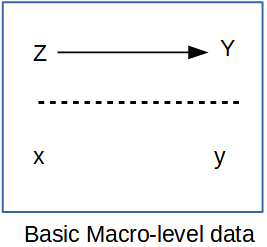
\includegraphics{images/macro2.png}

}

\caption{Macro Level Proposition}

\end{figure}

Such \textbf{macro-level propositions} are hypothesized relationships
among variables (\(\rightarrow\)) measured at a macro scale (\(Z\) and
\(Y\)), which ignores individual level data, mostly because we don't
observe individuals (\(x\) and \(y\)) in many of these kinds of
analysis.

If all we looked at were the individuals within the population, we would
be overwhelmed by the variation that we would see, and we wouldn't be
doing statistics anymore, we would be trying to process a million
anecdotes, and the plural of anecdote is not data. By aggregating across
basic demographic groups, such as age and sex, demographers begin to
tease apart the differences that we are interested in. If we go a little
further and, data willing, aggregate not only across these fundamental
demographic groups, but also across some kind of place-based areal unit,
then we adding an extremely important part of human existence: the
\textbf{where} part of where we live.

This presents an attractive view of populations and typically data on
places are more widely available, but there are caveats we must be aware
of. If we are using purely aggregate data in our analysis, meaning that
we do not have access to the individual level microdata, then our
ability to observe variation within a place is extremely limited, if not
impossible.

The goal of this chapter is to illustrate how places are a special unit
of analysis, and the types of data we often see at the place level are
very different from individual level surveys. Additionally, the analysis
of place-based data is similar to survey data in that places are do not
necessarily represent random observations, and so analyzing data on
places often requires special modifications to statistical models. In
this chapter, I show how the the linear regression model can be expanded
in several ways and illustrate the generalized linear model as a very
useful and extendable tool to analyze data on places and especially when
we are analyzing rates as demographers often do.

\hypertarget{getting-data-on-places}{%
\section{Getting data on places}\label{getting-data-on-places}}

In the macro-demographic perspective on demography, observations are
typically places, areas, or some other aggregate level of individuals.
We do not observe the individual people themselves often times. An
example of this is if you were to have access to an aggregate count of
deaths in a region, even if the deaths were classified by age and sex,
you still would be dealing with data that ignores, or has no index to
the more nuanced characteristics of the individual decedents themselves.
That being said, data such as these are invaluable, and most demographic
summaries of individual-level data would aggregate based on the
characteristics of the individuals any way. The macro scale principal is
illustrated below, where all of the variables we observe are a scale
above the individual person.

\begin{figure}

{\centering 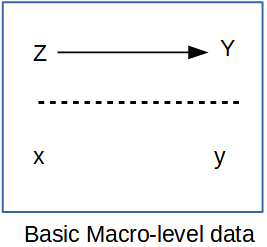
\includegraphics{images/macro2.png}

}

\caption{Macro Level Proposition}

\end{figure}

Such \textbf{macro-level propositions} are hypothesized relationships
among variables (\(\rightarrow\)) measured at a macro scale (\(Z\) and
\(Y\)), which ignores individual level data, mostly because we don't
observe individuals (\(x\) and \(y\)) in many of these kinds of
analysis.

If all we looked at were the individuals within the population, we would
be overwhelmed by the variation that we would see, and we wouldn't be
doing statistics anymore, we would be trying to process a million
anecdotes, and the plural of anecdote is not data. By aggregating across
basic demographic groups, such as age and sex, demographers begin to
tease apart the differences that we are interested in. If we go a little
further and, data willing, aggregate not only across these fundamental
demographic groups, but also across some kind of place-based areal unit,
then we adding an extremely important part of human existence: the
\textbf{where} part of where we live.

This presents an attractive view of populations and typically data on
places are more widely available, but there are caveats we must be aware
of. If we are using purely aggregate data in our analysis, meaning that
we do not have access to the individual level microdata, then our
ability to observe variation within a place is extremely limited, if not
impossible.

The goal of this chapter is to illustrate how places are a special unit
of analysis, and the types of data we often see at the place level are
very different from individual level surveys. Additionally, the analysis
of place-based data is similar to survey data in that places are do not
necessarily represent random observations, and so analyzing data on
places often requires special modifications to statistical models. In
this chapter, I show how the the linear regression model can be expanded
in several ways and illustrate the generalized linear model as a very
useful and extendable tool to analyze data on places and especially when
we are analyzing rates as demographers often do.

\hypertarget{getting-data-on-places-1}{%
\section{Getting data on places}\label{getting-data-on-places-1}}

Typically when thinking about data on places, we are really referring to
some sort of administrative geography, such as nations, states, region,
and census tracts. While these are often readily available (and I'll
show some R package that can easily get data from the web), we often
have to use these as proxy measures of more interesting social spaces
like neighborhoods and other types of activity spaces. These social
spaces are harder to get data on, typically because they are more fluid
in their definitions, and there is generally not a systematic effort to
produce data on socially defined spaces on national scales. This is a
big part of doing macro demography, defining the scale and the unit of
analysis, both because we need to define the scope of our work, but also
we are very much constrained by the availability of data for our
projects. For instance, I may want to look at national scale inequality
in mortality risk in neighborhoods in the United States, but you
immediately face a couple of hurdles. No national data source identifies
sub-city residential location for death certificates, also, what are
neighborhoods? Again, they're probably some socially defined space that
may not be available from a national scale source. To get around this,
we may have to settle for a state-level analysis, because state vital
registration systems will often allow researchers to use more fine-scale
geographic data on death certificates (such as latitude/longitude of the
decedent's residence), and once we have very fine scale geographic data
on the vital events, we could potentially find data on some more
socially defined spaces, perhaps from cities who often maintain
geographic data on neighborhoods specific to that city. OK, so that's
fine, but then you still run into the ``what's my denominator'' problem,
where you have no baseline population data on the age and sex breakdown
of the population, or even the population size of these places, because
federal agencies don't produce estimates for such small scale areas.
\emph{This is frustrating}. Often when advising students on their
dissertation projects, I have to have this moment of truth where I lay
out the problems of the mixing of geographic scales for their projects,
and the hard reality of the lack of data on so many things they would
like to study. Often what happens is that we have to proxy our ideal
places with places for which we can find data. You see this a lot in the
population health literature, where people want to analyze
\emph{neighborhoods} but all they have are census tracts. Tracts aren't
social spaces! They're arbitrary areas of 3 to 5 thousand people, that
change every 10 years, that the Census uses to count people. Likewise,
counties are very rich areas to find data for, but they are not really
activity spaces or neighborhoods, but they may be areas that have some
policy making authority (such as county health departments) that
\emph{could} be relevant for something. States are also nice
geographies, they're very large, so you loose the ability to
contextualize behavior on a fine spatial scale, but states make a lot of
decisions that affect the lives of their residents, often more than
national decisions. States have become very popular units of analysis in
the health literature again, primarily as a result of differential
adoption of portions of the Patient Protection and Affordable Care Act
of 2010 (Soni, Hendryx, and Simon 2017; Courtemanche et al. 2019). This
being said, many times when we do an analysis on places, that analysis
has lots of limitations, which we must acknowledge, and analyses such as
these are often called \emph{ecological} analyses because we are
examining associations at the macro scale, and we do not observe
individual level outcomes.

\hypertarget{us-contexts}{%
\section{US contexts}\label{us-contexts}}

The US Census bureau produces a wide variety of geographic data products
that are the most widely used forms of geographic data for demographic
studies in the United States. The TIGER Line Files data consist of
geographic data with census bureau GEOIDs attached so they can be linked
to any number of federal statistical products. They do not contain
demographic data themselves, but are easily linked. The \texttt{tigris}
package in R provides a direct way to download any TIGER line file data
type directly in a R session as either a \emph{simple feature} class or
as a \emph{Spatial\_DataFrame} (Walker 2021).

Using the \texttt{tigris} package is very easy and its functions fit
directly into the tidyverse as well. Below, I download two layers of
information, first the state polygon for New York state, and the census
tracts within the state and overlay the two datasets on each other. The
package has a function for each type of geography that you would want,
for example \texttt{states()} downloads state level geographies and
\texttt{tracts()} does the same for census tracts. The functions have
some common arguments, including \texttt{cb\ =\ TRUE/FALSE} so you can
choose cartographic boundary files or not. Cartographic boundary files
are lower resolution, smaller files that are often used for thematic
mapping. Also \texttt{year\ =} will allow you to get different annual
vintages of the data. The \texttt{tracts()} function also allows you to
obtain geographies for specific counties within a state.

\begin{Shaded}
\begin{Highlighting}[]
\FunctionTok{library}\NormalTok{(tigris)}

\NormalTok{nyst }\OtherTok{\textless{}{-}} \FunctionTok{states}\NormalTok{(}\AttributeTok{cb =} \ConstantTok{TRUE}\NormalTok{,}
               \AttributeTok{year =} \DecValTok{2010}\NormalTok{) }\SpecialCharTok{\%\textgreater{}\%}
  \FunctionTok{filter}\NormalTok{(NAME }\SpecialCharTok{==} \StringTok{"New York"}\NormalTok{)}

\NormalTok{nyst\_ct }\OtherTok{\textless{}{-}} \FunctionTok{tracts}\NormalTok{(}\AttributeTok{state =} \StringTok{"NY"}\NormalTok{,}
                  \AttributeTok{cb =} \ConstantTok{TRUE}\NormalTok{,}
                  \AttributeTok{year =} \DecValTok{2010}\NormalTok{)}

\FunctionTok{ggplot}\NormalTok{(}\AttributeTok{data=}\NormalTok{nyst)}\SpecialCharTok{+}
  \FunctionTok{geom\_sf}\NormalTok{(}\AttributeTok{color =} \StringTok{"red"}\NormalTok{, }
          \AttributeTok{lwd =} \DecValTok{2}\NormalTok{)}\SpecialCharTok{+}
   \FunctionTok{geom\_sf}\NormalTok{(}\AttributeTok{data =}\NormalTok{ nyst\_ct,}
           \AttributeTok{fill =} \ConstantTok{NA}\NormalTok{,}
           \AttributeTok{color =} \StringTok{"blue"}\NormalTok{) }\SpecialCharTok{+} 
  \FunctionTok{ggtitle}\NormalTok{(}\AttributeTok{label =} \StringTok{"New York State Census Tracts"}\NormalTok{)}
\end{Highlighting}
\end{Shaded}

\begin{figure}[H]

{\centering 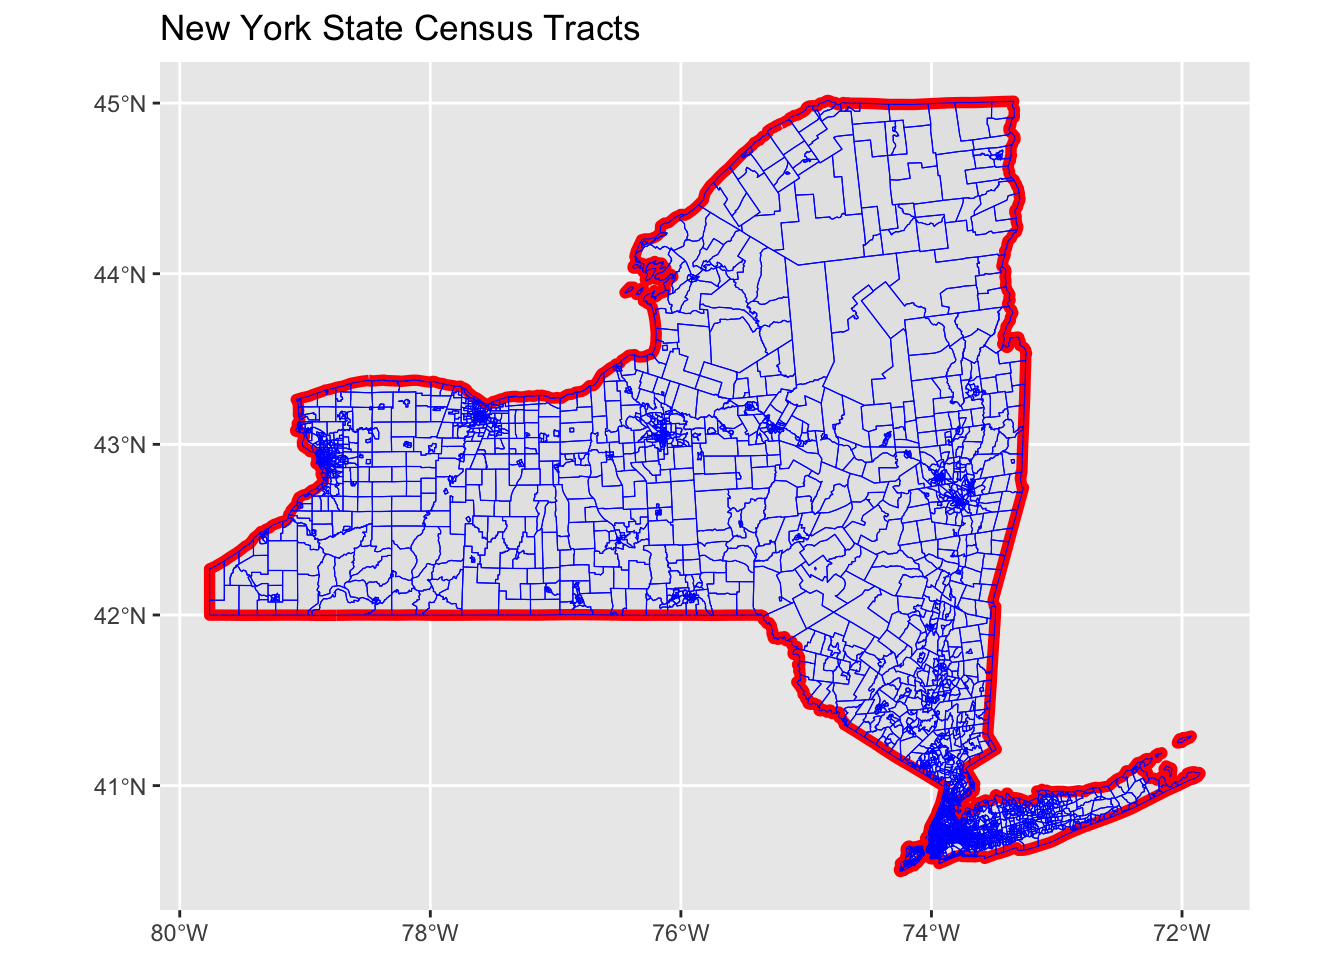
\includegraphics{macro_files/figure-pdf/unnamed-chunk-3-1.pdf}

}

\end{figure}

\hypertarget{tidycensus}{%
\subsection{Tidycensus}\label{tidycensus}}

Another package the provides access to the US Census Bureau Decennial
census summary file , the American Community Survey, Census population
estimates, migration flow data and Census Public Use Microdata Sample
(PUMS) data is \texttt{tidycensus} (Walker and Herman 2021). The
\texttt{tidycensus} package primarily works to allow users to use the
Census Bureau's Application Programming Interface (API) to download
Census summary file data for places within an R session. This removes
the need to download separate files to your computer, and allows users
to produce visualizations of Census data easily. The package is actively
maintained and has several online tutorials on how to use it
\footnote{\(\bar{y}= \text{mean of y}\), \(\bar{x}= \text{mean of x}\)}.
Depending on which data source you are interested in, there are
functions that allow extracts from them. The ACS data is accessed
through the \texttt{get\_acs()} function, likewise the decennial census
data is accessed using the \texttt{get\_decennial()} function. The
package also allows users to test for differences in ACS estimates
either across time or between areas using the \texttt{significance()}
function.

The package requires users to obtain a developer API key from the Census
Bureau's developer page\footnote{http://api.census.gov/data/key\_signup.html}
and install it on your local computer. The package has a function that
helps you install the key to your \texttt{.Renviron} file. It is used
like this:

\begin{Shaded}
\begin{Highlighting}[]
\FunctionTok{census\_api\_key}\NormalTok{(}\AttributeTok{key =} \StringTok{"yourkeyhere"}\NormalTok{, }\AttributeTok{install =} \ConstantTok{TRUE}\NormalTok{)}
\end{Highlighting}
\end{Shaded}

which only needs to be done once.

A basic use of the \texttt{tidycensus} package is to get data and
produce maps of the indicators. This is done easily because
\texttt{tidycensus} fits directly into general \texttt{dplyr} and
\texttt{ggplot2} workflows. Below is an example of accessing 2019 ACS
data on poverty rate estimates for New York census tracts from New York
county, New York. The syntax takes several arguments indicating what
level of census geography you want, the year of the estimates, the
details of states and counties you may want, and which ACS tables you
want. Here I use the Data Profile table for the percentage estimate of
families with incomes below the poverty line. The
\texttt{output\ =\ "wide"} option is useful if you get multiple
estimates, as it arranges them into columns, one for each estimate.

\begin{Shaded}
\begin{Highlighting}[]
\FunctionTok{library}\NormalTok{(tidycensus)}

\NormalTok{nyny }\OtherTok{\textless{}{-}} \FunctionTok{get\_acs}\NormalTok{(}\AttributeTok{geography =} \StringTok{"tract"}\NormalTok{,}
                \AttributeTok{year =} \DecValTok{2018}\NormalTok{,}
                \AttributeTok{state =} \StringTok{"NY"}\NormalTok{,}
                \AttributeTok{county =} \StringTok{"061"}\NormalTok{,}
                \AttributeTok{variables =} \StringTok{"DP03\_0119PE"}\NormalTok{, }
                \AttributeTok{output =} \StringTok{"wide"}\NormalTok{,}
                \AttributeTok{geometry =} \ConstantTok{TRUE}\NormalTok{)}
\end{Highlighting}
\end{Shaded}

\begin{verbatim}
Getting data from the 2014-2018 5-year ACS
\end{verbatim}

\begin{verbatim}
Downloading feature geometry from the Census website.  To cache shapefiles for use in future sessions, set `options(tigris_use_cache = TRUE)`.
\end{verbatim}

\begin{verbatim}
Using the ACS Data Profile
\end{verbatim}

The tabular output shows the Estimate column ending in \emph{E} and the
ACS margin of error column ending in \emph{M}.

\begin{Shaded}
\begin{Highlighting}[]
\NormalTok{knitr}\SpecialCharTok{::}\FunctionTok{kable}\NormalTok{(}\AttributeTok{x =} \FunctionTok{head}\NormalTok{(nyny),}
             \AttributeTok{format =} \StringTok{"html"}\NormalTok{)}
\end{Highlighting}
\end{Shaded}

\begin{longtable}[]{@{}llrrl@{}}
\toprule\noalign{}
GEOID & NAME & DP03\_0119PE & DP03\_0119PM & geometry \\
\midrule\noalign{}
\endhead
\bottomrule\noalign{}
\endlastfoot
36061020101 & Census Tract 201.01, New York County, New York & 0.0 &
20.0 & MULTIPOLYGON (((-73.96155 4... \\
36061020701 & Census Tract 207.01, New York County, New York & 24.1 &
17.0 & MULTIPOLYGON (((-73.95922 4... \\
36061022200 & Census Tract 222, New York County, New York & 18.5 & 9.1 &
MULTIPOLYGON (((-73.95068 4... \\
36061022600 & Census Tract 226, New York County, New York & 15.5 & 9.4 &
MULTIPOLYGON (((-73.94703 4... \\
36061000600 & Census Tract 6, New York County, New York & 37.5 & 9.8 &
MULTIPOLYGON (((-73.99256 4... \\
36061001600 & Census Tract 16, New York County, New York & 22.2 & 8.5 &
MULTIPOLYGON (((-73.99606 4... \\
\end{longtable}

The \texttt{geometry\ =\ TRUE} option also download the TIGER line file
for the requested geography and merges it to the ACS estimates. This
allows you to immediately map the estimates for the requested
geographies.

\begin{Shaded}
\begin{Highlighting}[]
\CommentTok{\# Create map of estimates}
\NormalTok{nyny }\SpecialCharTok{\%\textgreater{}\%} 
  \FunctionTok{rename}\NormalTok{ (}\AttributeTok{Poverty\_Rt =}\NormalTok{ DP03\_0119PE)}\SpecialCharTok{\%\textgreater{}\%}
  \FunctionTok{ggplot}\NormalTok{(}\FunctionTok{aes}\NormalTok{(}\AttributeTok{fill =}\NormalTok{ Poverty\_Rt))}\SpecialCharTok{+}
  \FunctionTok{geom\_sf}\NormalTok{()}\SpecialCharTok{+}
  \FunctionTok{scale\_fill\_viridis\_c}\NormalTok{()}\SpecialCharTok{+}
  \FunctionTok{ggtitle}\NormalTok{ ( }\AttributeTok{label =} \StringTok{"Poverty Rate in New York Census Tracts"}\NormalTok{, }
            \AttributeTok{subtitle =} \StringTok{"2018 ACS Estimates"}\NormalTok{)}
\end{Highlighting}
\end{Shaded}

\begin{figure}[H]

{\centering 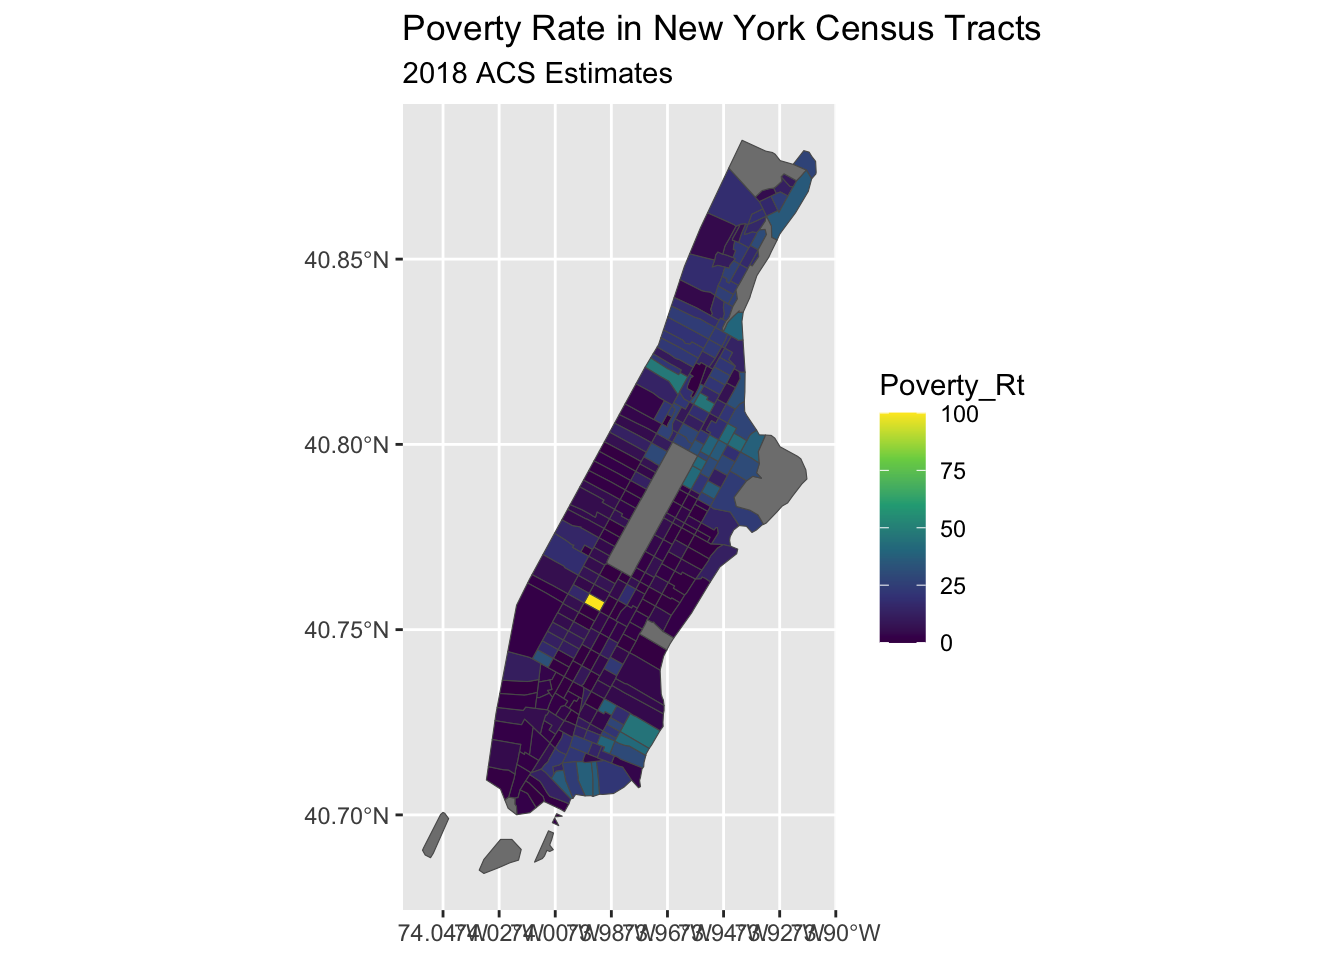
\includegraphics{macro_files/figure-pdf/unnamed-chunk-8-1.pdf}

}

\end{figure}

The \texttt{tidycensus} package had a great array of functions and the
author Kyle Walker has published a book on using it \emph{FILL IN
CITATION} which covers its many uses.

One common task that we should do when visualizing ACS estimates is to
examine the coefficient of variation in the estimates. This gives us an
idea of how stable the estimates are. This can be particularly
problematic as we use smaller and smaller geographies in our analysis.
Below, I calculate the coefficient of variation for the estimates and
map it. To get the standard error of the ACS estimate, I divide the
margin of error by 1.645, following Census Bureau recommendations
(Bureau 2019).

\begin{Shaded}
\begin{Highlighting}[]
\NormalTok{nyny }\SpecialCharTok{\%\textgreater{}\%} 
  \FunctionTok{mutate}\NormalTok{ ( }\AttributeTok{cv =}\FunctionTok{ifelse}\NormalTok{(}\AttributeTok{test =}\NormalTok{ DP03\_0119PE}\SpecialCharTok{==}\DecValTok{0}\NormalTok{,}
                      \AttributeTok{yes =} \DecValTok{0}\NormalTok{,}
                      \AttributeTok{no =}\NormalTok{ (DP03\_0119PM}\SpecialCharTok{/}\FloatTok{1.645}\NormalTok{) }\SpecialCharTok{/}\NormalTok{ DP03\_0119PE))}\SpecialCharTok{\%\textgreater{}\%}
  \FunctionTok{ggplot}\NormalTok{(}\FunctionTok{aes}\NormalTok{(}\AttributeTok{fill =}\NormalTok{ cv))}\SpecialCharTok{+}
  \FunctionTok{geom\_sf}\NormalTok{()}\SpecialCharTok{+}
  \FunctionTok{scale\_fill\_viridis\_c}\NormalTok{()}\SpecialCharTok{+}
  \FunctionTok{ggtitle}\NormalTok{ ( }\AttributeTok{label =} \StringTok{"Poverty Rate Coefficient of Variation}\SpecialCharTok{\textbackslash{}n}\StringTok{ in New York Census Tracts"}\NormalTok{, }
            \AttributeTok{subtitle =} \StringTok{"2018 ACS Estimates"}\NormalTok{)}
\end{Highlighting}
\end{Shaded}

\begin{figure}[H]

{\centering 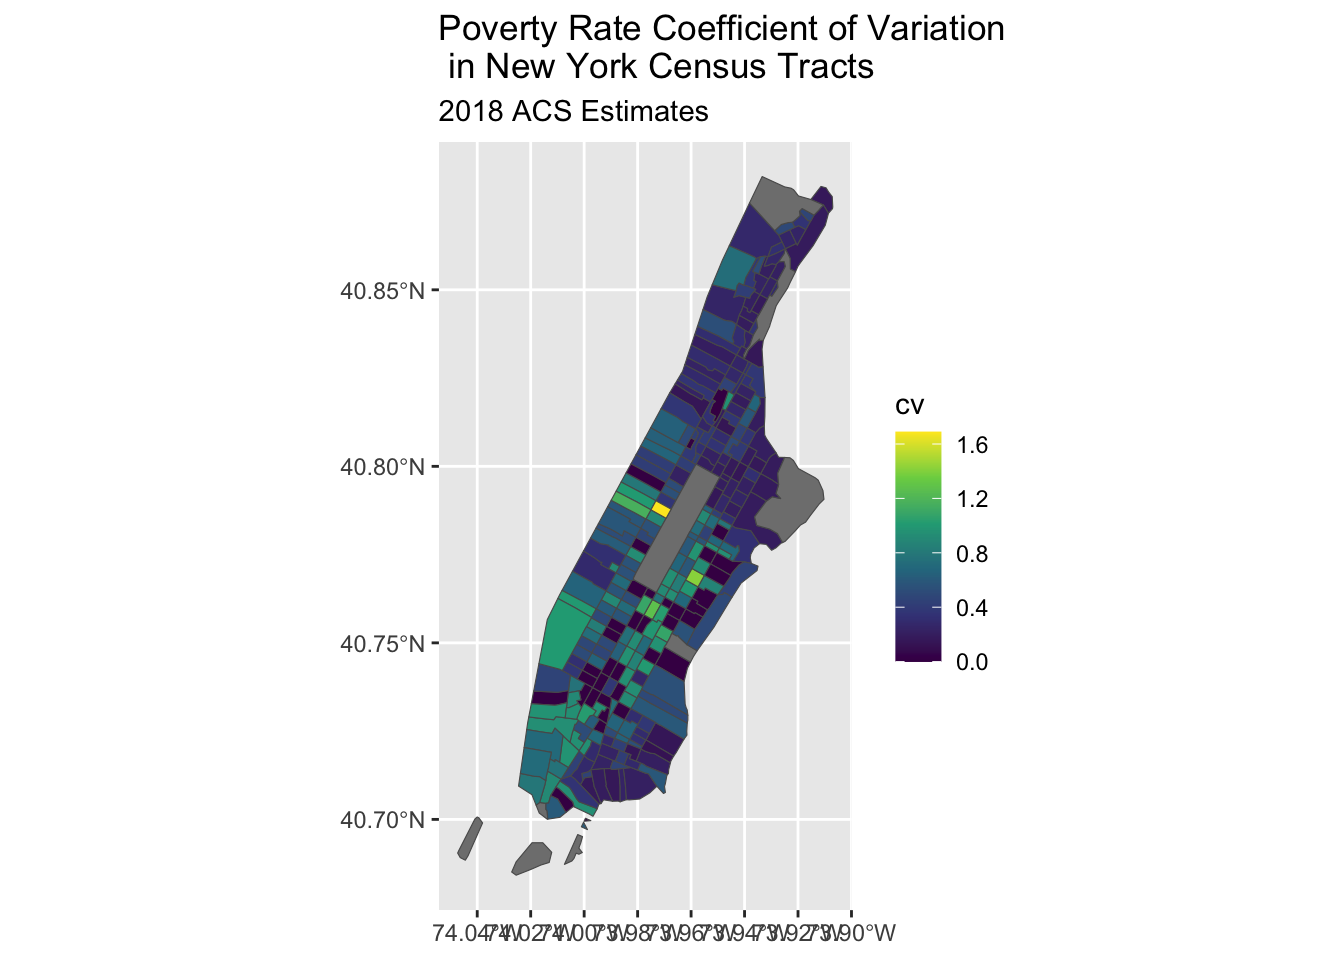
\includegraphics{macro_files/figure-pdf/unnamed-chunk-9-1.pdf}

}

\end{figure}

which shows areas with the highest coefficient of variations mostly
adjacent to Central Park and on the lower west side of Manhattan. These
are also the areas with the lowest poverty rates in the city, so the
estimates have low precision because so few respondents report incomes
below the poverty line.

\hypertarget{ipums-nhgis}{%
\subsection{IPUMS NHGIS}\label{ipums-nhgis}}

The IPUMS NHGIS project \footnote{Link to AHRF codebook -
  \href{https://data.hrsa.gov/DataDownload/AHRF/AHRF_USER_TECH_2019-2020.zip}{``https://data.hrsa.gov/DataDownload/AHRF/AHRF\_USER\_TECH\_2019-2020.zip''}}
is also a great source for demographic data on US places, and allows you
to select many demographic tables for census data products going back to
the 1790 census (Manson et al. 2021). When you perform an extract from
the site, you can get both data tables and ESRI shapefiles for your
requested geographies. The IPUMS staff have created several tutorials
which go through how to construct a query from their site \footnote{More
  on this below}. Below, I use the \texttt{sf} library to read in the
geographic data from IPUMS and the tabular data and join them.

\begin{Shaded}
\begin{Highlighting}[]
\FunctionTok{library}\NormalTok{(sf)}
\NormalTok{ipums\_co }\OtherTok{\textless{}{-}} \FunctionTok{read\_sf}\NormalTok{(}\StringTok{"data/US\_county\_2020.shp"}\NormalTok{)}


\NormalTok{im\_dat }\OtherTok{\textless{}{-}}\NormalTok{ readr}\SpecialCharTok{::}\FunctionTok{read\_csv}\NormalTok{(}\StringTok{"data/nhgis0025\_ds231\_2005\_county.csv"}\NormalTok{)}
\end{Highlighting}
\end{Shaded}

\begin{verbatim}
Rows: 3143 Columns: 12
-- Column specification --------------------------------------------------------
Delimiter: ","
chr (7): GISJOIN, AREANAME, STATE, STATEA, COUNTY, COUNTYA, DATAFLAG
dbl (5): YEAR, NOTECODE, AGWE001, AGWI001, AGWJ001

i Use `spec()` to retrieve the full column specification for this data.
i Specify the column types or set `show_col_types = FALSE` to quiet this message.
\end{verbatim}

\begin{Shaded}
\begin{Highlighting}[]
\NormalTok{m\_dat }\OtherTok{\textless{}{-}} \FunctionTok{left\_join}\NormalTok{(}\AttributeTok{x =}\NormalTok{ ipums\_co,}
                   \AttributeTok{y =}\NormalTok{ im\_dat,}
                   \AttributeTok{by =} \FunctionTok{c}\NormalTok{(}\StringTok{"GISJOIN"} \OtherTok{=} \StringTok{"GISJOIN"}\NormalTok{))}

\NormalTok{m\_dat }\SpecialCharTok{\%\textgreater{}\%}
  \FunctionTok{filter}\NormalTok{(STATE }\SpecialCharTok{==} \StringTok{"New York"}\NormalTok{ )}\SpecialCharTok{\%\textgreater{}\%}
  \FunctionTok{ggplot}\NormalTok{()}\SpecialCharTok{+}
  \FunctionTok{geom\_sf}\NormalTok{(}\FunctionTok{aes}\NormalTok{ (}\AttributeTok{fill =}\NormalTok{ AGWJ001))}\SpecialCharTok{+}
  \FunctionTok{scale\_fill\_viridis\_c}\NormalTok{()}\SpecialCharTok{+}
  \FunctionTok{ggtitle}\NormalTok{(}\AttributeTok{label =} \StringTok{"Infant Mortality Rate per 10,000 Live Births"}\NormalTok{,}
          \AttributeTok{subtitle =} \StringTok{"New York, 2005"}\NormalTok{)}
\end{Highlighting}
\end{Shaded}

\begin{figure}[H]

{\centering 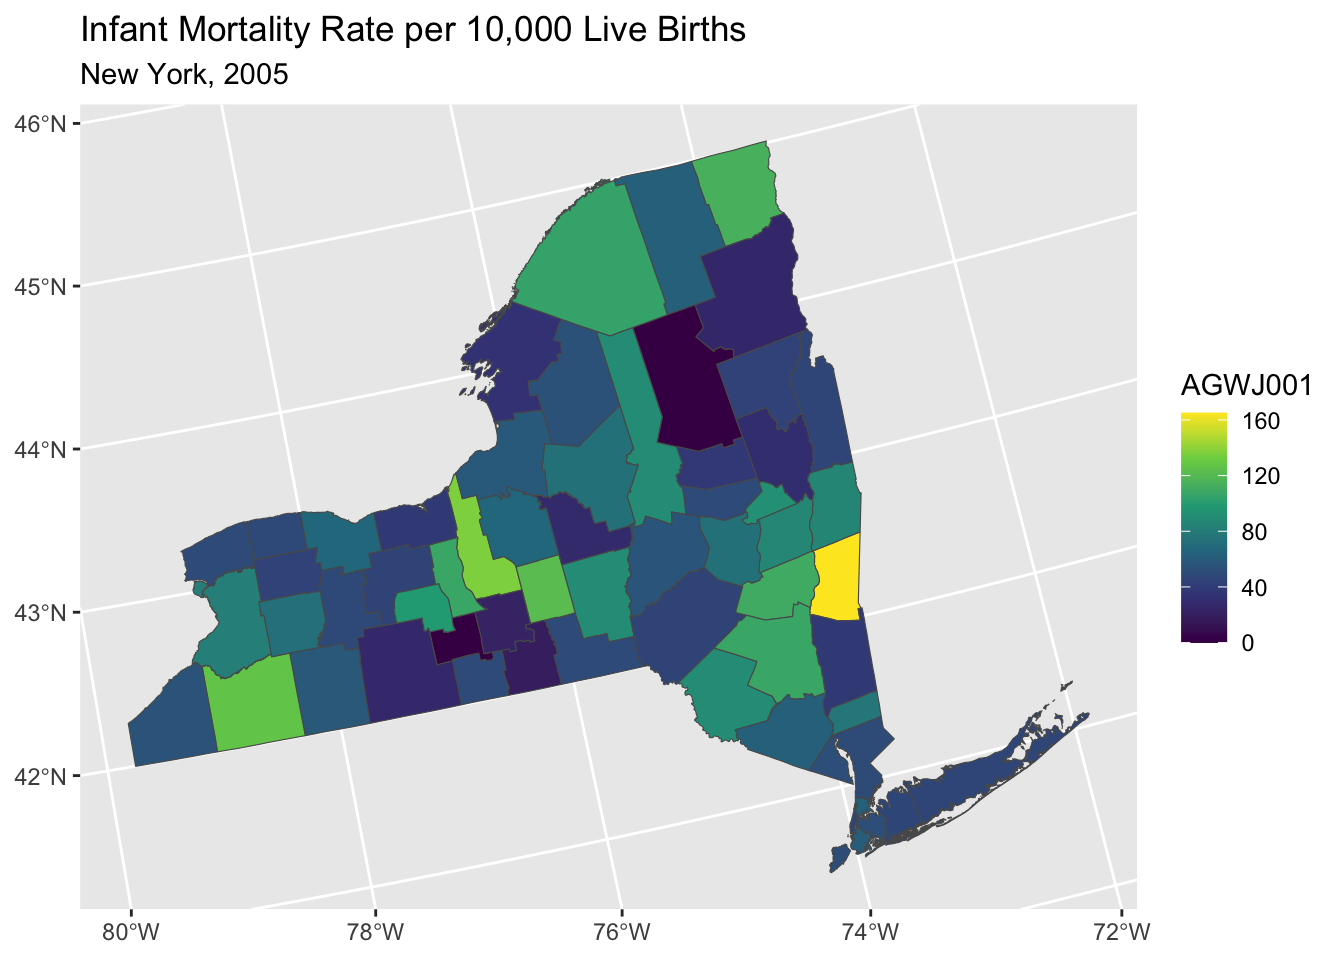
\includegraphics{macro_files/figure-pdf/unnamed-chunk-10-1.pdf}

}

\end{figure}

\hypertarget{international-data}{%
\subsection{International data}\label{international-data}}

Sources of international data exist in numerous sites on the internet.
Personally, I frequently will use the DHS Spatial Data repository
\footnote{More on this below} to access data from DHS sampled countries.
This repository allows you to obtain both spatial administrative
boundary data, as well as key indicators of maternal and child health at
sub-national levels. Additionally, the \texttt{rdhs} package allows you
to perform queries from the spatial data repository and from the DHS
microdata as well directly via the DHS API from within an R session
(Watson, FitzJohn, and Eaton 2019), assuming you have registered with
the DHS and have an approved project with them.

\hypertarget{statistical-models-for-place-based-data}{%
\section{Statistical models for place-based
data}\label{statistical-models-for-place-based-data}}

Data on places is often analysed in the same ways as data on
individuals, with some notable complications. The remainder of this
chapter introduces the regression framework for analyzing data at the
macro level, first by a review of the linear model and its associated
pitfalls, and then the generalized linear model with a specific focus on
the analysis of demographic count outcomes that are commonly observed
for places.

In the example below, I use data from the U.S. Health Resources and
Services Administration Area Health Resource File (AHRF), which is a
produced annually and includes a wealth of information on current and
historical data on health infrastructure in U.S. counties, as well as
data from the Census Bureau, and the National Center for Health
Statistics. The AHRF is publicly available, and we can read the data
directly from the HHS website as a SAS format \texttt{.sas7bdat} data
set within a ZIP archive. R can read this file to your local computer
then extract it using the commands below. I would strongly encourage you
consulting the AHRF codebook available from the HRSA website\footnote{Link
  to AHRF codebook -
  \href{https://data.hrsa.gov/DataDownload/AHRF/AHRF_USER_TECH_2019-2020.zip}{``https://data.hrsa.gov/DataDownload/AHRF/AHRF\_USER\_TECH\_2019-2020.zip''}}.

\begin{Shaded}
\begin{Highlighting}[]
\CommentTok{\#create temporary file on  your computer}
\NormalTok{temp }\OtherTok{\textless{}{-}} \FunctionTok{tempfile}\NormalTok{()}

\CommentTok{\#Download the SAS dataset as a ZIP compressed archive}
\FunctionTok{download.file}\NormalTok{(}\StringTok{"https://data.hrsa.gov/DataDownload/AHRF/AHRF\_2019{-}2020\_SAS.zip"}\NormalTok{, temp)}

\CommentTok{\#Read SAS data into R}
\NormalTok{ahrf}\OtherTok{\textless{}{-}}\NormalTok{haven}\SpecialCharTok{::}\FunctionTok{read\_sas}\NormalTok{(}\FunctionTok{unz}\NormalTok{(temp,}
                          \AttributeTok{filename =} \StringTok{"ahrf2020.sas7bdat"}\NormalTok{))}

\FunctionTok{rm}\NormalTok{(temp)}
\end{Highlighting}
\end{Shaded}

Next, I remove many of the variables in the AHRF and recode several
others. In the analysis examples that follow in this chapter, I will
focus on the outcome of low birth weight births, measured at the county
level.

\begin{Shaded}
\begin{Highlighting}[]
\FunctionTok{library}\NormalTok{(tidyverse)}

\NormalTok{ahrf2}\OtherTok{\textless{}{-}}\NormalTok{ahrf}\SpecialCharTok{\%\textgreater{}\%}
  \FunctionTok{mutate}\NormalTok{(}\AttributeTok{cofips =}\NormalTok{ f00004, }
         \AttributeTok{coname =}\NormalTok{ f00010,}
         \AttributeTok{state =}\NormalTok{ f00011,}
         \AttributeTok{popn =}\NormalTok{  f1198416,}
         \AttributeTok{births1618 =}\NormalTok{  f1254616, }
         \AttributeTok{lowbw1618 =}\NormalTok{ f1255316,}
         \AttributeTok{fampov14 =}\NormalTok{  f1443214,}
         \AttributeTok{lbrate1618 =} \DecValTok{1000}\SpecialCharTok{*}\NormalTok{(f1255316}\SpecialCharTok{/}\NormalTok{f1254616),  }\CommentTok{\#Rate per 1000 births}
         \AttributeTok{rucc =} \FunctionTok{as.factor}\NormalTok{(f0002013),}
         \AttributeTok{hpsa16 =} \FunctionTok{case\_when}\NormalTok{(.}\SpecialCharTok{$}\NormalTok{f0978716 }\SpecialCharTok{==} \DecValTok{0} \SpecialCharTok{\textasciitilde{}} \StringTok{\textquotesingle{}no shortage\textquotesingle{}}\NormalTok{,}
\NormalTok{                            .}\SpecialCharTok{$}\NormalTok{f0978716 }\SpecialCharTok{==} \DecValTok{1} \SpecialCharTok{\textasciitilde{}} \StringTok{\textquotesingle{}whole county shortage\textquotesingle{}}\NormalTok{,}
\NormalTok{                            .}\SpecialCharTok{$}\NormalTok{f0978716 }\SpecialCharTok{==} \DecValTok{2} \SpecialCharTok{\textasciitilde{}} \StringTok{\textquotesingle{}partial county shortage\textquotesingle{}}\NormalTok{),}
         \AttributeTok{obgyn15\_pc=} \DecValTok{1000}\SpecialCharTok{*}\NormalTok{( f1168415 }\SpecialCharTok{/}\NormalTok{ f1198416 ) )}\SpecialCharTok{\%\textgreater{}\%}
  \FunctionTok{mutate}\NormalTok{(}\AttributeTok{rucc =} \FunctionTok{droplevels}\NormalTok{(rucc, }\StringTok{""}\NormalTok{))}\SpecialCharTok{\%\textgreater{}\%}
\NormalTok{  dplyr}\SpecialCharTok{::}\FunctionTok{select}\NormalTok{(births1618,}
\NormalTok{                lowbw1618,}
\NormalTok{                lbrate1618,}
\NormalTok{                state,}
\NormalTok{                cofips,}
\NormalTok{                coname,}
\NormalTok{                popn,}
\NormalTok{                fampov14,}
\NormalTok{                rucc,}
\NormalTok{                hpsa16,}
\NormalTok{                obgyn15\_pc)}\SpecialCharTok{\%\textgreater{}\%}
  \FunctionTok{filter}\NormalTok{(}\FunctionTok{complete.cases}\NormalTok{(.))}\SpecialCharTok{\%\textgreater{}\%}
  \FunctionTok{as.data.frame}\NormalTok{()}
\end{Highlighting}
\end{Shaded}

In order to make a nice looking map of the outcome, I use the
\texttt{tigris} package to fetch geographic data for US states and
counties, then merge the county data to the AHRF data using
\texttt{left\_join()}

\begin{Shaded}
\begin{Highlighting}[]
\FunctionTok{options}\NormalTok{(}\AttributeTok{tigris\_class=}\StringTok{"sf"}\NormalTok{)}
\FunctionTok{library}\NormalTok{(tigris)}
\FunctionTok{library}\NormalTok{(sf)}
\NormalTok{usco}\OtherTok{\textless{}{-}}\FunctionTok{counties}\NormalTok{(}\AttributeTok{cb =}\NormalTok{ T, }\AttributeTok{year=} \DecValTok{2016}\NormalTok{)}

\NormalTok{usco}\SpecialCharTok{$}\NormalTok{cofips}\OtherTok{\textless{}{-}}\NormalTok{usco}\SpecialCharTok{$}\NormalTok{GEOID}

\NormalTok{sts}\OtherTok{\textless{}{-}}\FunctionTok{states}\NormalTok{(}\AttributeTok{cb =}\NormalTok{ T, }\AttributeTok{year =} \DecValTok{2016}\NormalTok{)}

\NormalTok{sts}\OtherTok{\textless{}{-}}\FunctionTok{st\_boundary}\NormalTok{(sts)}\SpecialCharTok{\%\textgreater{}\%}
  \FunctionTok{filter}\NormalTok{(}\SpecialCharTok{!}\NormalTok{STATEFP }\SpecialCharTok{\%in\%} \FunctionTok{c}\NormalTok{(}\StringTok{"02"}\NormalTok{, }\StringTok{"15"}\NormalTok{, }\StringTok{"60"}\NormalTok{, }\StringTok{"66"}\NormalTok{, }\StringTok{"69"}\NormalTok{, }\StringTok{"72"}\NormalTok{, }\StringTok{"78"}\NormalTok{))}\SpecialCharTok{\%\textgreater{}\%}
  \FunctionTok{st\_transform}\NormalTok{(}\AttributeTok{crs =} \DecValTok{2163}\NormalTok{)}

\NormalTok{ahrf\_m}\OtherTok{\textless{}{-}}\FunctionTok{left\_join}\NormalTok{(usco, ahrf2,}
                    \AttributeTok{by =} \StringTok{"cofips"}\NormalTok{)}\SpecialCharTok{\%\textgreater{}\%}
  \FunctionTok{filter}\NormalTok{(}\FunctionTok{is.na}\NormalTok{(lbrate1618)}\SpecialCharTok{==}\NormalTok{F, }
         \SpecialCharTok{!}\NormalTok{STATEFP }\SpecialCharTok{\%in\%} \FunctionTok{c}\NormalTok{(}\StringTok{"02"}\NormalTok{, }\StringTok{"15"}\NormalTok{, }\StringTok{"60"}\NormalTok{, }\StringTok{"66"}\NormalTok{, }\StringTok{"69"}\NormalTok{, }\StringTok{"72"}\NormalTok{, }\StringTok{"78"}\NormalTok{))}\SpecialCharTok{\%\textgreater{}\%}
  \FunctionTok{st\_transform}\NormalTok{(}\AttributeTok{crs =} \DecValTok{2163}\NormalTok{)}

\FunctionTok{glimpse}\NormalTok{(ahrf\_m)}
\end{Highlighting}
\end{Shaded}

There are a total of 2,418 observations in the data, because the HRSA
restricts some counties with small numbers of births from the data.

Here is a \texttt{ggplot()} histogram of the low birth weight rate for
US counties.

\begin{Shaded}
\begin{Highlighting}[]
\NormalTok{ahrf\_m}\SpecialCharTok{\%\textgreater{}\%}
  \FunctionTok{ggplot}\NormalTok{()}\SpecialCharTok{+}
  \FunctionTok{geom\_histogram}\NormalTok{(}\FunctionTok{aes}\NormalTok{(}\AttributeTok{x =}\NormalTok{ lbrate1618))}\SpecialCharTok{+}
  \FunctionTok{labs}\NormalTok{(}\AttributeTok{title =} \StringTok{"Distribution of Low Birth Weight Rates in US Counties"}\NormalTok{,}
       \AttributeTok{subtitle =} \StringTok{"2016 {-} 2018"}\NormalTok{)}\SpecialCharTok{+}
       \FunctionTok{xlab}\NormalTok{(}\StringTok{"Rate per 1,000 Live Births"}\NormalTok{)}\SpecialCharTok{+}
  \FunctionTok{ylab}\NormalTok{ (}\StringTok{"Frequency"}\NormalTok{)}
\end{Highlighting}
\end{Shaded}

\begin{verbatim}
`stat_bin()` using `bins = 30`. Pick better value with `binwidth`.
\end{verbatim}

\begin{figure}[H]

{\centering 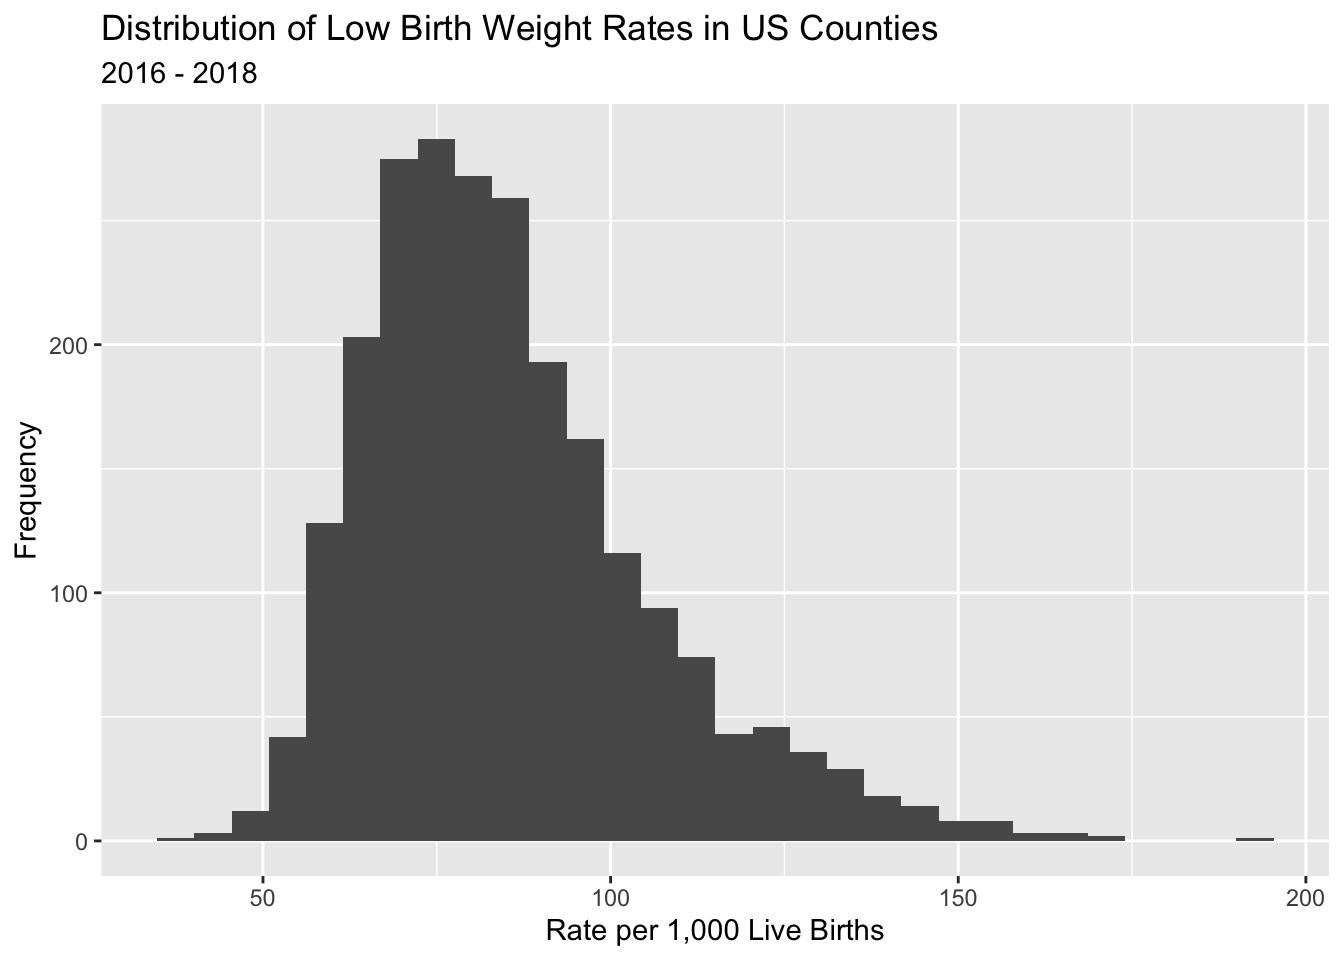
\includegraphics{macro_files/figure-pdf/unnamed-chunk-14-1.pdf}

}

\end{figure}

Here, we do a basic map of the outcome variable for the continental US,
and see the highest rates of low birth weight births in the US occur in
the southeastern areas of the country. Notice, I do not color the
boundaries of the counties in order to maximize the reader's ability to
see the variation, instead I show lines between states by overlaying the
\texttt{sts} layer from above. I also add cartographic options of a
scale bar and a north arrow, which I personally believe should be on any
map shown to the public.

\begin{Shaded}
\begin{Highlighting}[]
\FunctionTok{library}\NormalTok{(tmap)}

\FunctionTok{tm\_shape}\NormalTok{(ahrf\_m)}\SpecialCharTok{+}
  \FunctionTok{tm\_polygons}\NormalTok{(}\AttributeTok{col =} \StringTok{"lbrate1618"}\NormalTok{,}
              \AttributeTok{border.col =} \ConstantTok{NULL}\NormalTok{,}
              \AttributeTok{title=}\StringTok{"Low Birth Weight Rt"}\NormalTok{,}
              \AttributeTok{palette=}\StringTok{"Blues"}\NormalTok{,}
              \AttributeTok{style=}\StringTok{"quantile"}\NormalTok{,}
              \AttributeTok{n=}\DecValTok{5}\NormalTok{,}
              \AttributeTok{showNA=}\NormalTok{T, }\AttributeTok{colorNA =} \StringTok{"grey50"}\NormalTok{)}\SpecialCharTok{+}
   \FunctionTok{tm\_format}\NormalTok{(}\AttributeTok{format=} \StringTok{"World"}\NormalTok{,}
             \AttributeTok{main.title=}\StringTok{"US Low Birth Weight Rate by County"}\NormalTok{,}
            \AttributeTok{legend.position =}  \FunctionTok{c}\NormalTok{(}\StringTok{"left"}\NormalTok{, }\StringTok{"bottom"}\NormalTok{),}
            \AttributeTok{main.title.position =}\FunctionTok{c}\NormalTok{(}\StringTok{"center"}\NormalTok{))}\SpecialCharTok{+}
  \FunctionTok{tm\_scale\_bar}\NormalTok{(}\AttributeTok{position =} \FunctionTok{c}\NormalTok{(.}\DecValTok{1}\NormalTok{,}\DecValTok{0}\NormalTok{))}\SpecialCharTok{+}
  \FunctionTok{tm\_compass}\NormalTok{()}\SpecialCharTok{+}
\FunctionTok{tm\_shape}\NormalTok{(sts)}\SpecialCharTok{+}
  \FunctionTok{tm\_lines}\NormalTok{( }\AttributeTok{col =} \StringTok{"black"}\NormalTok{)}
\end{Highlighting}
\end{Shaded}

\begin{figure}[H]

{\centering 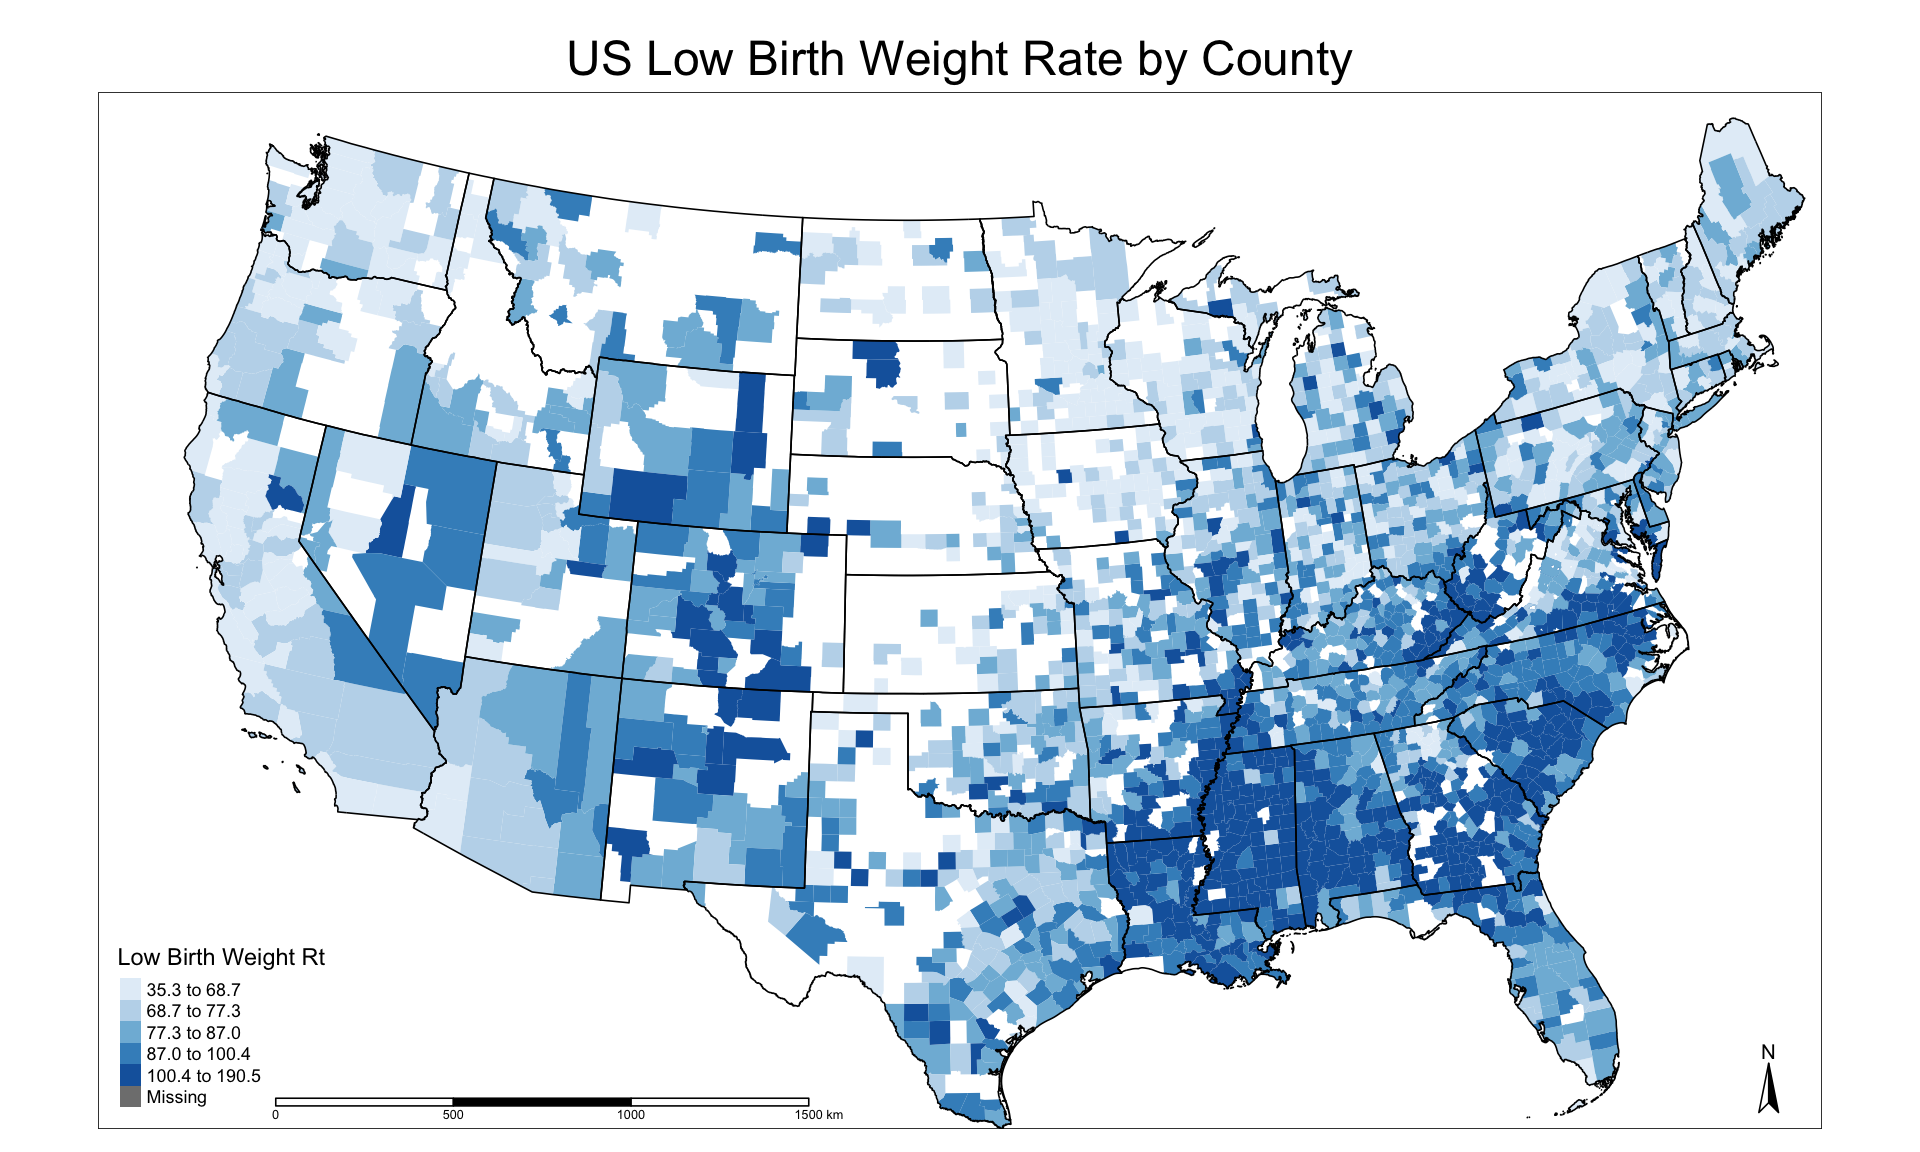
\includegraphics{macro_files/figure-pdf/unnamed-chunk-15-1.pdf}

}

\end{figure}

When doing analysis of place-based data, maps are almost a fundamental
aspect of the analysis and often convey much more information about the
distribution of the outcome than either distribution plots or summary
statistics.

\hypertarget{the-linear-model-framework}{%
\section{The linear model framework}\label{the-linear-model-framework}}

Probably the most used and often abused statistical model is the linear
regression model, sometimes called the OLS model because it is typically
estimated by the method of least squares. I do not plan on spending a
lot of real estate in this this book talking about the linear model,
mostly because lots of times it doesn't get us very far, and there are
much more thorough books on this subject, one of my personal favorites
being John Fox's text on applied regression (Fox 2016).

This model is typically shown as:

\[y_i = \beta_0 +\sum_k \beta_k x_{ki} + \epsilon_i\]

with the \(\beta\)'s being parameters that define the linear
relationship between the independent variables \(x_k\), and \(y\), and
\(\epsilon_i\) being the unexplained, or residual portion of \(y\) that
is included in the model. The model has several assumptions that we need
to worry about, first being normality of the residuals, or

\[\epsilon_i \sim Normal(0, \sigma_\epsilon)\]

Where \(\sigma_\epsilon ^2\) is the residual variance, or mean square
error of the model. Under the strict assumptions of the linear model,
the Gauss-Markov theorem says that the unbiased and minimum variance
estimates of the \(\beta\)'s is:

\[
\beta_k = \frac{\sum (y_i - \bar{y})(x_i - \bar{x})}{\sum x_i - \bar{x}^2} = \frac{Cov(x,y)}{Var(x)}
\]

Which is often shown in the more compact matrix form:

\[\beta_k = (X'X)^{-1} X'Y\]

We could just as directly write the model in it's distributional form
as:

\[
y_i \sim Normal(\beta_0 +\sum_k \beta_k x_{ki}, \sigma_\epsilon)
\]

or even as:

\[
y_i \sim Normal(X' \beta, \sigma_\epsilon)
\]

Which I prefer because it sets up the regression equation as the
\textbf{linear predictor}, or linear combination (in the linear algebra
sense) of the predictors and the model parameters for the mean of the
outcome. This term, linear predictor, is a useful one, because as you
get more and more accustomed to regression, you will see this same
structure in every regression model you ever do. This is the fundamental
workhorse of regression, where we get an estimated value for every
combination of the observed predictors. Moreover, below when I present
the \textbf{Generalized Linear Model}, it will be apparent that the
linear predictor can be placed within a number of so-called \textbf{link
functions} to ensure that the mean of the outcome agrees with the
assumed distribution for the outcome.

\hypertarget{estimating-the-linear-model-in-r}{%
\section{Estimating the linear model in
R}\label{estimating-the-linear-model-in-r}}

The linear model is included in the base R \texttt{stats} package, and
is accessed by the \texttt{lm()} function. In the example below, I use
data from the U.S. Health Resources and Services Administration Area
Health Resource File (AHRF) to estimate a model of the associations
between the poverty rate, the rurality of the county and whether the
county is a healthcare shortage area. This is a mixture of continuous
(or partially continuous) and categorical predictors.

The basic \texttt{lm()} model syntax is specified as
\texttt{lm\ (\ y\ \textasciitilde{}\ x\_1\ +\ x\_2,\ data\ =\ dataname)}
with the \texttt{\textasciitilde{}} operator representing the formula
for the model equation, with the outcome on the left and the predictors
on the right. You also provide the name of the dataframe which contains
the variables specified in the formula in a \texttt{data=} argument. For
help on the function and to see the other potential arguments use
\texttt{?lm}.

\begin{Shaded}
\begin{Highlighting}[]
\NormalTok{lm1 }\OtherTok{\textless{}{-}} \FunctionTok{lm}\NormalTok{ (lbrate1618 }\SpecialCharTok{\textasciitilde{}}\NormalTok{  fampov14 }\SpecialCharTok{+}\NormalTok{ rucc }\SpecialCharTok{+}\NormalTok{ hpsa16, }\AttributeTok{data =}\NormalTok{ ahrf\_m)}
\end{Highlighting}
\end{Shaded}

This stores the model data and parameter estimates in the object called
\texttt{lm1}. You can name the object anything you wish, just try to
avoid using other R commands as object names. For instance, I wouldn't
want to call an object \texttt{mean} or \texttt{sd} because those are
names of functions. The basic way to see the model results is to use the
\texttt{summary()} function on the model fit.

\begin{Shaded}
\begin{Highlighting}[]
\FunctionTok{summary}\NormalTok{(lm1)}
\end{Highlighting}
\end{Shaded}

\begin{verbatim}

Call:
lm(formula = lbrate1618 ~ fampov14 + rucc + hpsa16, data = ahrf_m)

Residuals:
    Min      1Q  Median      3Q     Max 
-90.114 -10.345  -1.229   9.287  77.778 

Coefficients:
                              Estimate Std. Error t value Pr(>|t|)    
(Intercept)                   62.26920    1.18901  52.371  < 2e-16 ***
fampov14                       2.25805    0.06846  32.981  < 2e-16 ***
rucc02                        -1.91854    1.20082  -1.598 0.110249    
rucc03                        -3.38658    1.25055  -2.708 0.006818 ** 
rucc04                        -6.65483    1.40639  -4.732 2.36e-06 ***
rucc05                        -5.96283    1.93739  -3.078 0.002110 ** 
rucc06                        -3.94180    1.14317  -3.448 0.000575 ***
rucc07                        -4.00730    1.28166  -3.127 0.001790 ** 
rucc08                         0.45112    2.11062   0.214 0.830770    
rucc09                        -3.88365    2.29118  -1.695 0.090202 .  
hpsa16partial county shortage -0.66219    1.00767  -0.657 0.511148    
hpsa16whole county shortage    2.36214    1.25335   1.885 0.059601 .  
---
Signif. codes:  0 '***' 0.001 '**' 0.01 '*' 0.05 '.' 0.1 ' ' 1

Residual standard error: 16.36 on 2312 degrees of freedom
Multiple R-squared:  0.3697,    Adjusted R-squared:  0.3667 
F-statistic: 123.3 on 11 and 2312 DF,  p-value: < 2.2e-16
\end{verbatim}

We see that there is a significant positive association between family
poverty and the low birth weight rate, we also see that there is a
tendency for more rural areas to have lower low birth weight rates than
the largest cities (Reference level = \texttt{rucc01}). There is a
marginally significant association between a county being a healthcare
shortage area and the low birth weight rate. Overall the model is
explaining about a third of the variation in the outcome, as seen in the
adjusted R-Square value of .3667.

\hypertarget{a-not-on-interpretation}{%
\subsubsection{A not on interpretation}\label{a-not-on-interpretation}}

It is important to remember, when describing results for place-based
data, to avoid using language centered on individuals. For instance,
with reference to the \texttt{fampov14} variable, we cannot say that
families living in poverty are more likely to have a low birth weight
birth, instead, we must focus on discussion on \emph{places} with higher
rates of poverty having a higher rate of low birth weight births.
Ascribing individual risk from an ecological analysis is an example of
the \emph{ecological fallacy} often seen when doing place-based
analysis, and we must be aware of it when framing our questions and
describing our results.

The \texttt{gtsummary} package (Sjoberg et al. 2021) provides a very
nice interface to produce much better looking summaries of models.

\begin{Shaded}
\begin{Highlighting}[]
\FunctionTok{library}\NormalTok{(gtsummary)}

\NormalTok{lm1}\SpecialCharTok{\%\textgreater{}\%}
  \FunctionTok{tbl\_regression}\NormalTok{(}\AttributeTok{add\_estimate\_to\_reference\_rows =} \ConstantTok{TRUE}\NormalTok{)}
\end{Highlighting}
\end{Shaded}

\begin{verbatim}
Table printed with `knitr::kable()`, not {gt}. Learn why at
https://www.danieldsjoberg.com/gtsummary/articles/rmarkdown.html
To suppress this message, include `message = FALSE` in code chunk header.
\end{verbatim}

\begin{tabular}{l|c|c|c}
\hline
**Characteristic** & **Beta** & **95\% CI** & **p-value**\\
\hline
\% Families Below Poverty Level 2014-18 & 2.3 & 2.1, 2.4 & <0.001\\
\hline
rucc &  &  & \\
\hline
01 & 0.00 & — & \\
\hline
02 & -1.9 & -4.3, 0.44 & 0.11\\
\hline
03 & -3.4 & -5.8, -0.93 & 0.007\\
\hline
04 & -6.7 & -9.4, -3.9 & <0.001\\
\hline
05 & -6.0 & -9.8, -2.2 & 0.002\\
\hline
06 & -3.9 & -6.2, -1.7 & <0.001\\
\hline
07 & -4.0 & -6.5, -1.5 & 0.002\\
\hline
08 & 0.45 & -3.7, 4.6 & 0.8\\
\hline
09 & -3.9 & -8.4, 0.61 & 0.090\\
\hline
hpsa16 &  &  & \\
\hline
no shortage & 0.00 & — & \\
\hline
partial county shortage & -0.66 & -2.6, 1.3 & 0.5\\
\hline
whole county shortage & 2.4 & -0.10, 4.8 & 0.060\\
\hline
\end{tabular}

\hypertarget{assumptions-of-the-ols-model}{%
\section{Assumptions of the OLS
model}\label{assumptions-of-the-ols-model}}

The linear model has several assumptions that we need to be concerned
with, the big four are

\begin{enumerate}
\def\labelenumi{\arabic{enumi})}
\tightlist
\item
  \emph{Normality of residuals},
\item
  \emph{Constant variance in residuals, or}
  \emph{\emph{homoskedasticity}}, and
\item
  \emph{Linearity of the regression function}, and
\item
  \emph{Independence of observations}
\end{enumerate}

The normality assumption is linked to distributional assumption
underlying the linear regression model. This states that the model
residuals, calculated as
\(e_i = (\beta_0 +\sum_k \beta_k x_{ki}) - y_i\), or more compactly as
\(e_i =\hat{y_i} - y_i\) follow a normal distribution. If the errors
around the mean function are not normally distributed, this can be an
indicator that the linear model is not appropriate for the outcome under
consideration. A commonly used graphical check of this is the
\emph{quantile-quantile} or Q-Q plot, which plots the residuals from a
model against the hypothetical quantiles from a normal distribution.

We can check these for our model above easily:

\begin{Shaded}
\begin{Highlighting}[]
\FunctionTok{hist}\NormalTok{(}\FunctionTok{residuals}\NormalTok{(lm1))}
\end{Highlighting}
\end{Shaded}

\begin{figure}[H]

{\centering 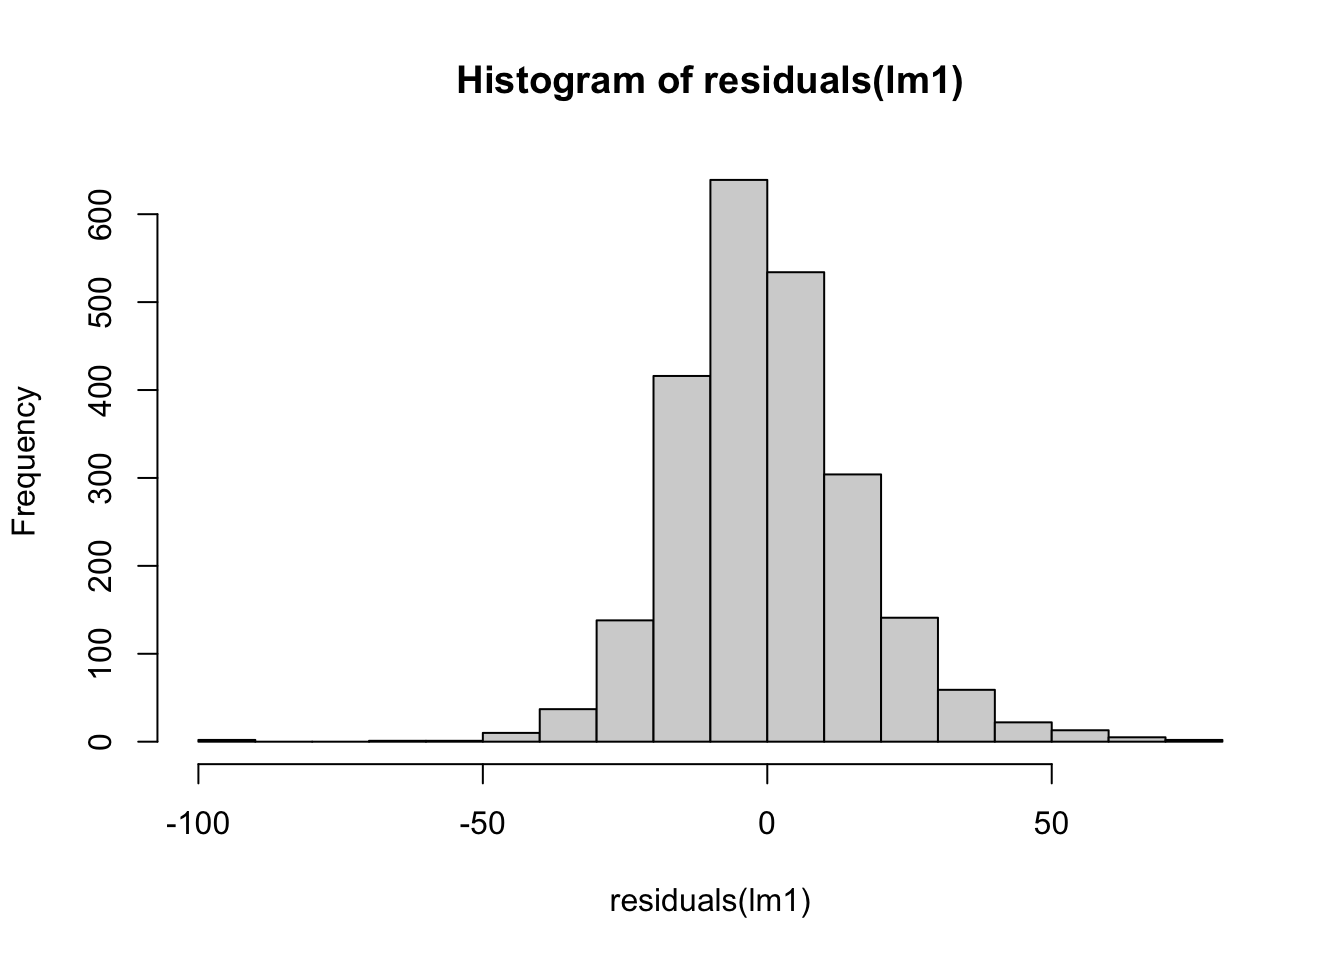
\includegraphics{macro_files/figure-pdf/unnamed-chunk-19-1.pdf}

}

\end{figure}

\begin{Shaded}
\begin{Highlighting}[]
\FunctionTok{plot}\NormalTok{(}\FunctionTok{density}\NormalTok{(}\FunctionTok{resid}\NormalTok{(lm1)),}
     \AttributeTok{main =} \StringTok{"Density plot of the residuals"}\NormalTok{)}
\FunctionTok{curve}\NormalTok{(}\FunctionTok{dnorm}\NormalTok{(x,}\DecValTok{0}\NormalTok{,}\FunctionTok{sd}\NormalTok{(}\FunctionTok{resid}\NormalTok{(lm1))),}
       \AttributeTok{col =} \StringTok{"blue"}\NormalTok{, }\AttributeTok{lwd =}\DecValTok{2}\NormalTok{, }\AttributeTok{add=}\ConstantTok{TRUE}\NormalTok{)}
\end{Highlighting}
\end{Shaded}

\begin{figure}[H]

{\centering 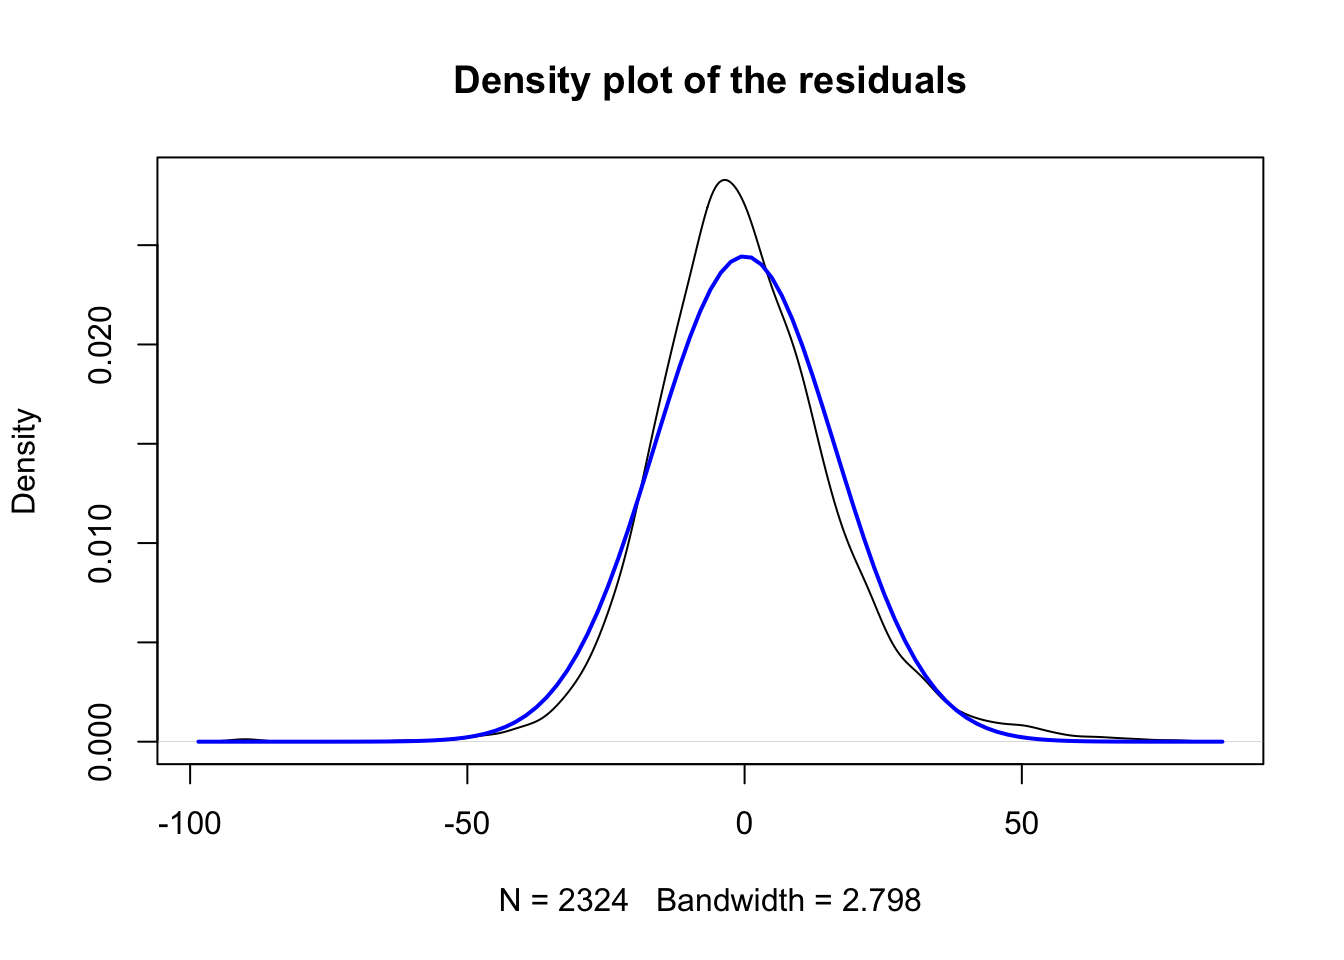
\includegraphics{macro_files/figure-pdf/unnamed-chunk-19-2.pdf}

}

\end{figure}

\begin{Shaded}
\begin{Highlighting}[]
\FunctionTok{plot}\NormalTok{(lm1, }\AttributeTok{which =} \DecValTok{2}\NormalTok{)}
\end{Highlighting}
\end{Shaded}

\begin{figure}[H]

{\centering 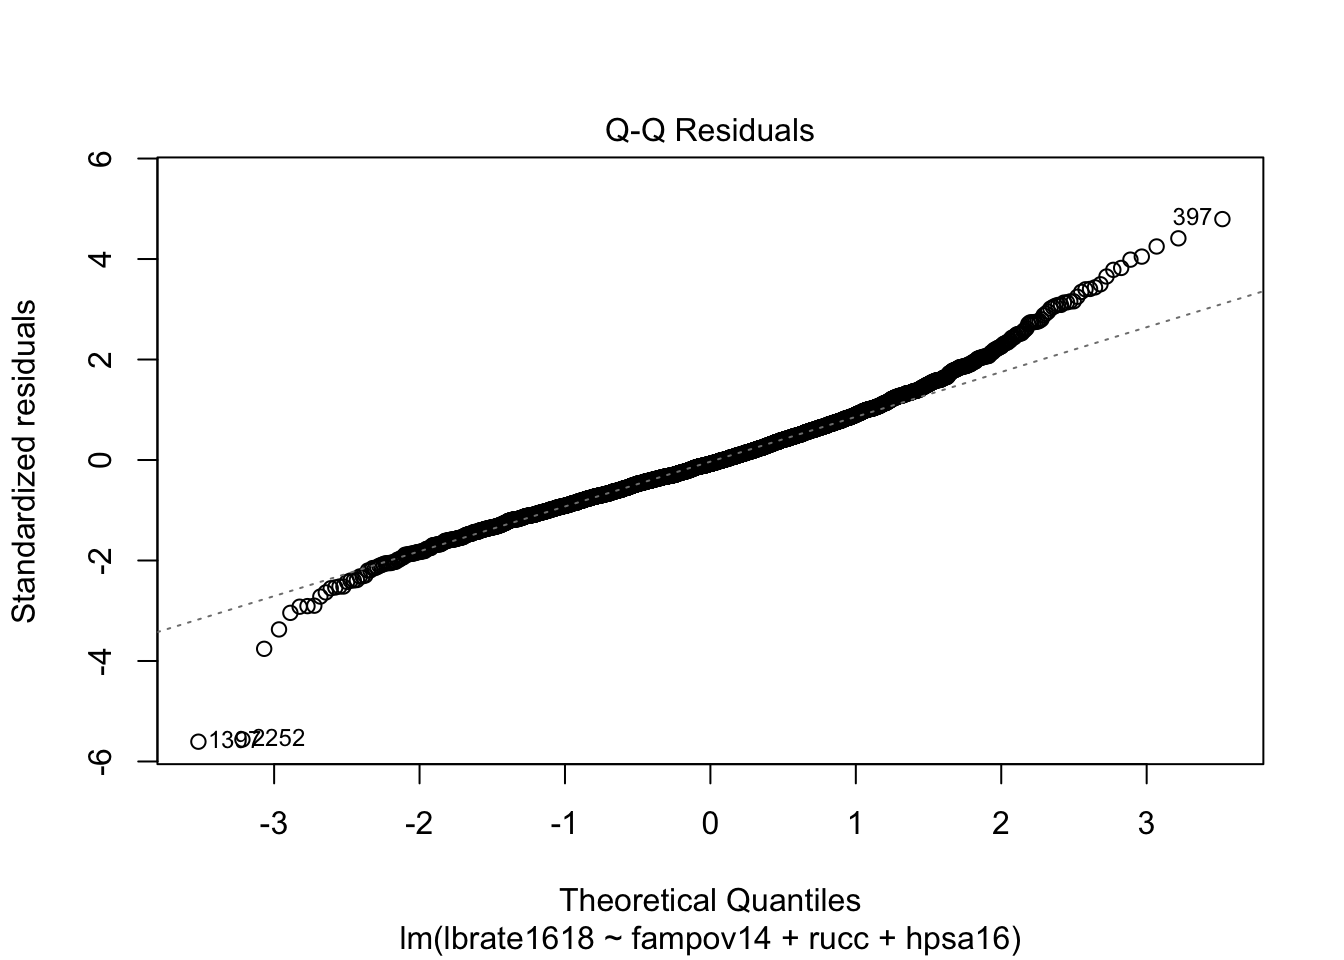
\includegraphics{macro_files/figure-pdf/unnamed-chunk-19-3.pdf}

}

\end{figure}

While the overall distribution of the residuals is fairly normal based
on the histogram and the comparison to the normal density plot, the q-q
plot shows that the tails of the distribution are not well modeled by
the normal distribution because there are several observations that are
too far below or above the theoretical line (dotted line).

The \emph{homoskedasticity} assumption is also tied to the normal
distributional assumption of the model, as see above, if we write the
model in its distributional form,
\(y_i \sim Normal(X' \beta, \sigma_\epsilon)\), the term \$
\sigma\_\epsilon\$ is a single parameter, meaning that we only have one
of these in a linear regression model. This parameter determines the
spread of the variation around the mean function. Larger values equal
more spread around the mean, and smaller values equal less spread. A
commonly used graphical procedure to detect lack of homoskedasticity, or
\emph{heteroskedasticity}, is an envelope plot, or a plot of the
residuals against the fitted values from the model. Formal tests also
exist including the \emph{Breusch-Pagan test} and the modified version
of this test developed by Cook and Weisberg {[}cite{]}

A graphical check of this assumption is easily done from the model fit:

\begin{Shaded}
\begin{Highlighting}[]
\FunctionTok{plot}\NormalTok{(lm1, }\AttributeTok{which =} \FunctionTok{c}\NormalTok{(}\DecValTok{1}\NormalTok{,}\DecValTok{3}\NormalTok{))}
\end{Highlighting}
\end{Shaded}

\begin{figure}[H]

{\centering 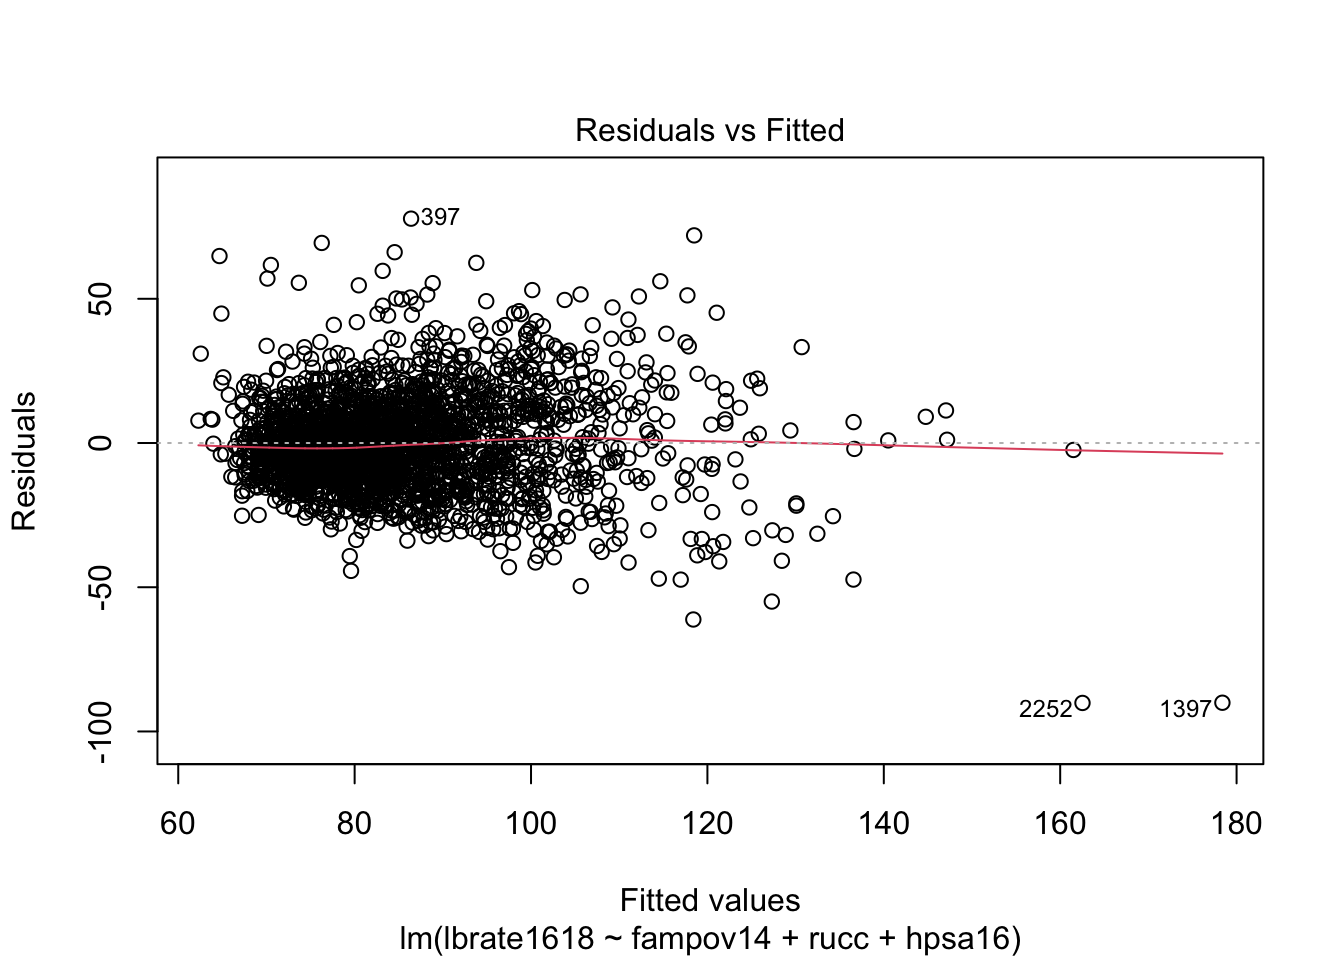
\includegraphics{macro_files/figure-pdf/unnamed-chunk-20-1.pdf}

}

\end{figure}

\begin{figure}[H]

{\centering 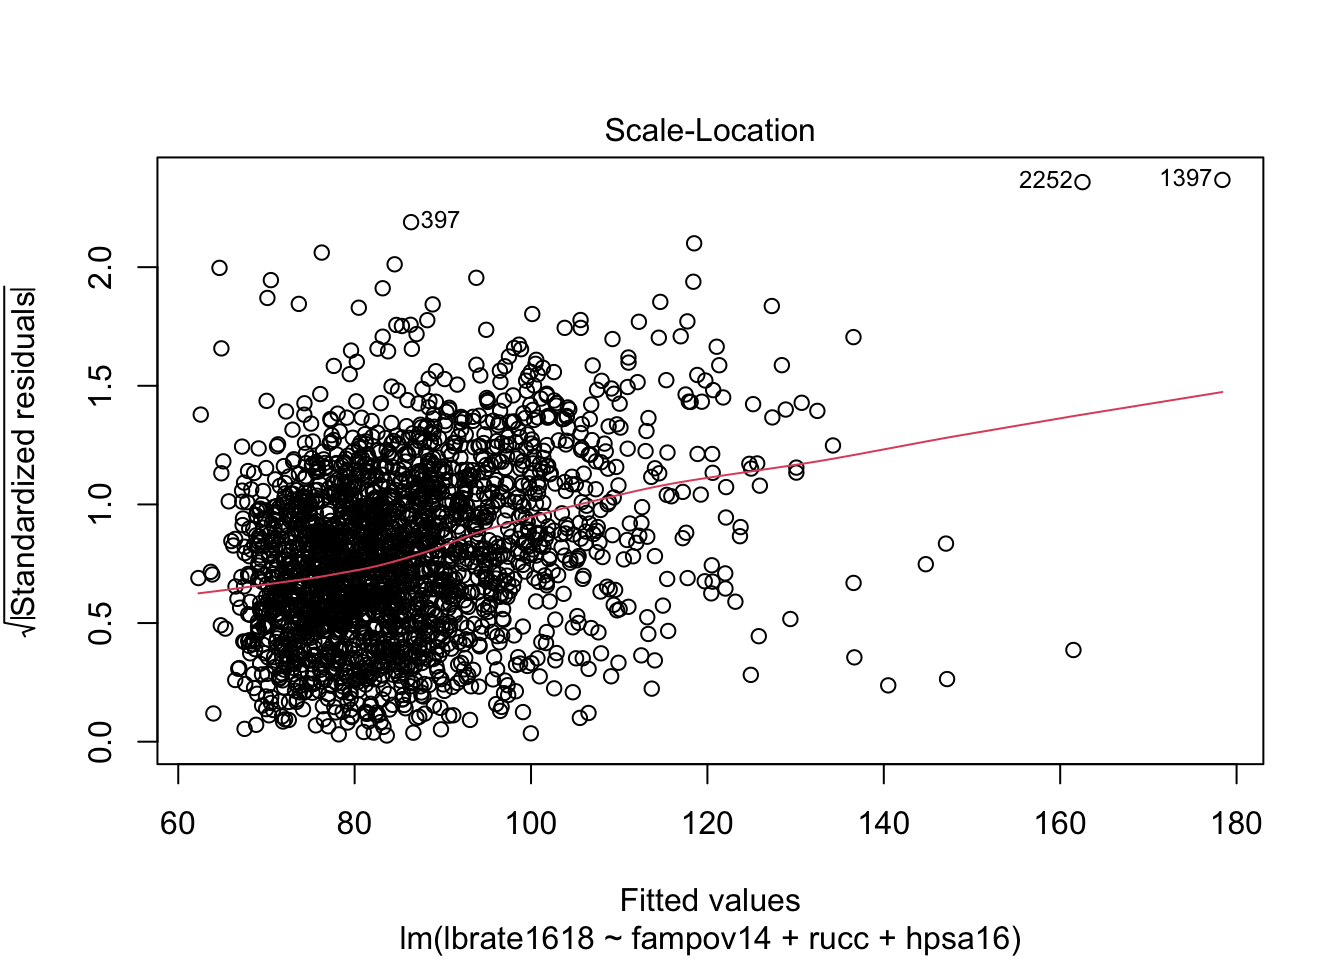
\includegraphics{macro_files/figure-pdf/unnamed-chunk-20-2.pdf}

}

\end{figure}

These plots show some evidence that the error variances are
non-constant. The first plot has the very characteristic ``fish'' or
``cone'' shape, where the error variances increase as the fitted values
increase. We can also do a formal test using functions from the
\texttt{car} package:

\begin{Shaded}
\begin{Highlighting}[]
\FunctionTok{library}\NormalTok{(car)}
\end{Highlighting}
\end{Shaded}

\begin{verbatim}
Loading required package: carData
\end{verbatim}

\begin{verbatim}

Attaching package: 'car'
\end{verbatim}

\begin{verbatim}
The following object is masked from 'package:dplyr':

    recode
\end{verbatim}

\begin{verbatim}
The following object is masked from 'package:purrr':

    some
\end{verbatim}

\begin{Shaded}
\begin{Highlighting}[]
\FunctionTok{ncvTest}\NormalTok{(lm1)}
\end{Highlighting}
\end{Shaded}

\begin{verbatim}
Non-constant Variance Score Test 
Variance formula: ~ fitted.values 
Chisquare = 469.4844, Df = 1, p = < 2.22e-16
\end{verbatim}

Which again shows more statistical evidence of the non-constant variance
in residuals.

\hypertarget{correction-for-non-constant-variance}{%
\subsubsection{Correction for non-constant
variance}\label{correction-for-non-constant-variance}}

The assumption of homoskedasticity is important for two reasons, first
is related to prediction from the model, but the second is related to
the test statistics derived from the model. In order to test our
hypothesis that \(x\) is related to \(y\), we form the ratio of the
\(\beta_1\) parameter to its error, this is typically either a \(z\),
\(t\) or Wald \(\chi^2\) statistic, depending on which procedure you're
using.

\[t = \frac{\hat{\beta_1}}{se(\beta_1))}\] The term \(se(\beta_1)\) is
the estimated standard error of the parameter, and is calculated using
the ratio of the residual standard deviation and the square root of the
sums of squares of the \(x\):

\[se(\beta_1) = \frac{\sigma_{\epsilon}}{\sqrt{\sum(x - \bar{x})^2}}\]

or in the matrix terms:

\[Var(\beta) = \sigma_{\epsilon}(X'X)^{-1}\]

if the term \(\sigma_{\epsilon}\) is not constant then the standard
error of each parameter in the model is incorrect. Corrections for
heteroskedasticity are commonplace in the social sciences, and are
usually attributed to White (1980) and MacKinnon and White (1985) with
many additions since the original publication, notably Long and Ervin
(2000). These corrections use the empirically observed error terms and
avoid the assumption of common variance in all residuals.

The \texttt{coeftest()} function in the \texttt{lmtest} package is one
option to correct for heteroskedasticity in regression models. It allows
for various correction types, with the ``HC3'' type (Long and Ervin
2000) being the default for linear models. Below, I show the default
tests assuming constant variance and the corrected tests.

\begin{Shaded}
\begin{Highlighting}[]
\FunctionTok{library}\NormalTok{(sandwich)}
\FunctionTok{library}\NormalTok{(lmtest)}
\end{Highlighting}
\end{Shaded}

\begin{verbatim}
Loading required package: zoo
\end{verbatim}

\begin{verbatim}

Attaching package: 'zoo'
\end{verbatim}

\begin{verbatim}
The following objects are masked from 'package:base':

    as.Date, as.Date.numeric
\end{verbatim}

\begin{Shaded}
\begin{Highlighting}[]
\FunctionTok{coeftest}\NormalTok{(lm1)}
\end{Highlighting}
\end{Shaded}

\begin{verbatim}

t test of coefficients:

                               Estimate Std. Error t value  Pr(>|t|)    
(Intercept)                   62.269198   1.189010 52.3706 < 2.2e-16 ***
fampov14                       2.258054   0.068465 32.9813 < 2.2e-16 ***
rucc02                        -1.918536   1.200819 -1.5977 0.1102488    
rucc03                        -3.386577   1.250553 -2.7081 0.0068176 ** 
rucc04                        -6.654825   1.406391 -4.7318 2.359e-06 ***
rucc05                        -5.962826   1.937392 -3.0778 0.0021101 ** 
rucc06                        -3.941799   1.143175 -3.4481 0.0005746 ***
rucc07                        -4.007304   1.281664 -3.1266 0.0017901 ** 
rucc08                         0.451120   2.110622  0.2137 0.8307703    
rucc09                        -3.883651   2.291182 -1.6950 0.0902020 .  
hpsa16partial county shortage -0.662194   1.007671 -0.6572 0.5111478    
hpsa16whole county shortage    2.362138   1.253348  1.8847 0.0596007 .  
---
Signif. codes:  0 '***' 0.001 '**' 0.01 '*' 0.05 '.' 0.1 ' ' 1
\end{verbatim}

\begin{Shaded}
\begin{Highlighting}[]
\FunctionTok{coeftest}\NormalTok{(lm1, }\AttributeTok{vcov  =} \FunctionTok{vcovHC}\NormalTok{(lm1, }\AttributeTok{type =} \StringTok{"HC3"}\NormalTok{))}
\end{Highlighting}
\end{Shaded}

\begin{verbatim}

t test of coefficients:

                              Estimate Std. Error t value  Pr(>|t|)    
(Intercept)                   62.26920    1.14941 54.1749 < 2.2e-16 ***
fampov14                       2.25805    0.11349 19.8966 < 2.2e-16 ***
rucc02                        -1.91854    0.97531 -1.9671 0.0492896 *  
rucc03                        -3.38658    1.06364 -3.1839 0.0014722 ** 
rucc04                        -6.65483    1.20922 -5.5034 4.137e-08 ***
rucc05                        -5.96283    1.95622 -3.0481 0.0023288 ** 
rucc06                        -3.94180    1.09704 -3.5931 0.0003336 ***
rucc07                        -4.00730    1.30130 -3.0795 0.0020981 ** 
rucc08                         0.45112    2.42803  0.1858 0.8526203    
rucc09                        -3.88365    3.29696 -1.1779 0.2389381    
hpsa16partial county shortage -0.66219    0.85442 -0.7750 0.4384068    
hpsa16whole county shortage    2.36214    1.26921  1.8611 0.0628553 .  
---
Signif. codes:  0 '***' 0.001 '**' 0.01 '*' 0.05 '.' 0.1 ' ' 1
\end{verbatim}

The take away in this example is that non-constant variance can affect
the standard errors of the model parameter estimates, and in turn affect
the test statistics that we base all of our hypothesis tests on. In the
particulars of this model there is not a lot of change, the
\texttt{rucc02} parameter is barley significant once using the corrected
standard errors, otherwise we see a very similar pattern in terms of
what is significant in the model.

\hypertarget{clustered-standard-errors}{%
\subsubsection{Clustered standard
errors}\label{clustered-standard-errors}}

Another commonly used correction in regression modeling is the
\emph{clustered standard error}. These are commonplace and almost the
default in the Stata programming environment, and are widely used in the
field of economics. Clustering of standard errors attempts to correct
for clustering in the residuals from the regression model. Clustering
can happen for a wide variety of reasons, and as we saw in the previous
chapter on survey data analysis, is often an artifact of how the data
are collected. With place-based data, we may have clustering because the
places are close to each other, or because the share some other
characteristic that we have not measured in our regression model. In the
case of our regression model, and in our descriptive analysis of our
outcome, the map shown prior may indicate some form of \emph{spatial
correlation} in the outcome. While there are models to deal with such
non-independence in place-based data, they are not a subject I will
touch on here. Instead, we may use the state which each county is in as
a proxy for the spatial clustering in the outcome, as one example of
potential of a clustering term.

\begin{Shaded}
\begin{Highlighting}[]
\FunctionTok{coeftest}\NormalTok{(lm1,}
         \AttributeTok{vcov  =} \FunctionTok{vcovCL}\NormalTok{(lm1, }\AttributeTok{cluster =}\NormalTok{ ahrf\_m}\SpecialCharTok{$}\NormalTok{state))}
\end{Highlighting}
\end{Shaded}

\begin{verbatim}

t test of coefficients:

                              Estimate Std. Error t value  Pr(>|t|)    
(Intercept)                   62.26920    2.43737 25.5477 < 2.2e-16 ***
fampov14                       2.25805    0.28830  7.8322 7.243e-15 ***
rucc02                        -1.91854    1.15345 -1.6633  0.096387 .  
rucc03                        -3.38658    1.42381 -2.3785  0.017462 *  
rucc04                        -6.65483    1.35050 -4.9277 8.912e-07 ***
rucc05                        -5.96283    2.60314 -2.2906  0.022075 *  
rucc06                        -3.94180    1.28117 -3.0767  0.002118 ** 
rucc07                        -4.00730    2.11299 -1.8965  0.058017 .  
rucc08                         0.45112    2.59621  0.1738  0.862069    
rucc09                        -3.88365    4.73238 -0.8207  0.411927    
hpsa16partial county shortage -0.66219    1.18695 -0.5579  0.576971    
hpsa16whole county shortage    2.36214    1.80407  1.3093  0.190549    
---
Signif. codes:  0 '***' 0.001 '**' 0.01 '*' 0.05 '.' 0.1 ' ' 1
\end{verbatim}

In this case, the \texttt{rucc02} and \texttt{rucc07} terms become
marginally significant and the healthcare shortage areas lose their
marginal significance.

\hypertarget{weighted-least-squares}{%
\subsubsection{Weighted Least Squares}\label{weighted-least-squares}}

Another method of dealing with non-constant error variance is the method
of weighted least squares. This method modifies the model somewhat to
be:

\[y \sim Normal(\beta_0 +\sum_k \beta_k x_{ki}, \sigma_{\epsilon_i} )\]

Where the term \(\sigma_{\epsilon_i}\) represents the different
variances for each observation. The weights in the model are often
variables that represent an underlying factor that affects the variance
in the estimates. In demography this is often the population size of a
place, as places with smaller population sizes often have more
volatility to their rate estimates. This approach has been used in the
spatial demographic modeling of county mortality rates in the United
States by several authors (McLaughlin et al. 2007; Sparks and Sparks
2010).

\begin{Shaded}
\begin{Highlighting}[]
\NormalTok{lm2 }\OtherTok{\textless{}{-}} \FunctionTok{lm}\NormalTok{(lbrate1618 }\SpecialCharTok{\textasciitilde{}}\NormalTok{  fampov14 }\SpecialCharTok{+}\NormalTok{ rucc }\SpecialCharTok{+}\NormalTok{ hpsa16,}
          \AttributeTok{data =}\NormalTok{ ahrf\_m,}
          \AttributeTok{weights =}\NormalTok{ popn)}
\FunctionTok{summary}\NormalTok{(lm2)}
\end{Highlighting}
\end{Shaded}

\begin{verbatim}

Call:
lm(formula = lbrate1618 ~ fampov14 + rucc + hpsa16, data = ahrf_m, 
    weights = popn)

Weighted Residuals:
   Min     1Q Median     3Q    Max 
-42957  -2122   -106   2333  27618 

Coefficients:
                              Estimate Std. Error t value Pr(>|t|)    
(Intercept)                   65.54503    0.98536  66.519  < 2e-16 ***
fampov14                       1.83332    0.06338  28.928  < 2e-16 ***
rucc02                        -0.63464    0.66623  -0.953 0.340901    
rucc03                        -1.67371    0.93793  -1.784 0.074479 .  
rucc04                        -4.38387    1.31520  -3.333 0.000872 ***
rucc05                        -3.31398    2.16308  -1.532 0.125642    
rucc06                        -1.87074    1.35213  -1.384 0.166630    
rucc07                        -2.12596    1.80385  -1.179 0.238693    
rucc08                         3.92060    4.33118   0.905 0.365452    
rucc09                        -0.21442    4.93030  -0.043 0.965315    
hpsa16partial county shortage -1.85070    0.93518  -1.979 0.047938 *  
hpsa16whole county shortage    0.21786    1.65417   0.132 0.895229    
---
Signif. codes:  0 '***' 0.001 '**' 0.01 '*' 0.05 '.' 0.1 ' ' 1

Residual standard error: 4620 on 2312 degrees of freedom
Multiple R-squared:  0.2832,    Adjusted R-squared:  0.2798 
F-statistic: 83.05 on 11 and 2312 DF,  p-value: < 2.2e-16
\end{verbatim}

We see that by including the population size weights in the model, most
of the parameters are no longer significant in the analysis, but the
weights have not dealt with the non-constant variance issue totally:

\begin{Shaded}
\begin{Highlighting}[]
\FunctionTok{ncvTest}\NormalTok{(lm2)}
\end{Highlighting}
\end{Shaded}

\begin{verbatim}
Non-constant Variance Score Test 
Variance formula: ~ fitted.values 
Chisquare = 84.49228, Df = 1, p = < 2.22e-16
\end{verbatim}

But the overall size of the non-constant variance test is much lower
than it was for the original model.

\hypertarget{linearity-assumption}{%
\subsection{Linearity assumption}\label{linearity-assumption}}

The linearity assumption of the model assumes that the true underlying
relationship in the data can be modeled using a linear combination of
the predictors and the parameters. I think a lot of people think this
means that you cannot include square or polynomial terms in a regression
model, but that is not the case. The assumption is concerned with the
linearity of the parameters, not the predictor variables themselves. For
example the standard linear model with one predictor, x is written:

\[y = \beta_0 + \beta_1 x_1 + \epsilon\]

Which is clearly the equation for a straight line with y-intercept
\(\beta_0\) and slope \(\beta_1\). We also see that the parameters
combine in a linear (additive) fashion. This is the assumption of the
model, and can also be seen when expressing this equation using vector
notation

\[y = x' \beta\]

Because the term \(x' \beta\) is the inner product of the \(\beta\)
parameters and the information from \(x\). If we include the square of
\(x\) in the model:

\[y = \beta_0 + \beta_1 x_1 + \beta_2 x_1^2 + \epsilon\] The same inner,
additive product of the \(\beta\)s and the \(x\)s is still the same. If
we constructed a model that was non-linear function of the \(\beta\)s,
such as:

\[y = \beta_0 + \beta_1 x_1 *  e^{\beta_2 x_1^2} + \epsilon\] The the
model would no longer be linear in the parameters because we introduce a
nonlinearity by exponentiating the \(\beta_2\) parameter inside the mean
function (not that this is a real model, just as an example).

When this actually comes into our experience is when our data are
actually generated by a nonlinear process, such as a time series with
seasonality included, which may oscillate between seasons (such as
temperature, or rainfall), for instance a situation such as this arises:

Where the variable y is actually generated from a cosine curve with
noise. Since the linear regression of y on x forces the y to change
linearly with x, the model is absolutely unable to recover the
underlying pattern in the data.

\textbf{A note on splines}

If the data clearly do not display a linear trend, I personally
automatically look to \emph{splines} as a means to model the
non-linearity in relationship. Splines are a method of constructing a
model based on connecting either linear or non-linear functions across a
series of breaks or \textbf{\emph{knots}} along the data in which the
form of the function changes.

Mathematically, knots can be written as:

\$\$ Y(x) =

\begin{Bmatrix}
F_1(x) \text {  for  } x\in [x_1, x_2]\\ 
F_2(x) \text {  for  } x\in [x_2, x_3]\\ 
\cdots \\ 
F_{k}(x) \text {  for  } x\in [x_{k-1}, x_k]\\

\end{Bmatrix}

\$\$

Where each of the \(F_k (x)\) functions imply a different form in the
interval between \(x\in [x_{k-1}, x_k]\), where the \(k\) breaks are at
a given knot in the data. Most splines are nonlinear functions, usually
cubic polynomials, and the spline model combines a series of these
polynomials to model nonlinearities in the relationship between
predictors and outcomes. A relatively recent invention,
\emph{Generalized Additive Models} or \emph{GAMs} are a way to model an
outcome with both linear and non-linear terms together. The GAM model
forms the linear predictor of a model can be constructed as:

\[E(y)= \beta_0 + f(x_1) + \beta_1 x_2\] where the \(f(x_1)\) term is a
regression spline of one of the variables. The models can be a mixture
of linear and smooth terms. Here is an example of using a B-spline
within the \texttt{lm()} model to fit a smooth regression function to
the messy nonlinear model above.

\begin{Shaded}
\begin{Highlighting}[]
\FunctionTok{library}\NormalTok{(splines)}

\NormalTok{sm}\OtherTok{\textless{}{-}} \FunctionTok{lm}\NormalTok{(y2}\SpecialCharTok{\textasciitilde{}}\FunctionTok{bs}\NormalTok{(t, }\AttributeTok{df =} \DecValTok{5}\NormalTok{))}

\FunctionTok{plot}\NormalTok{(t, y2, }\AttributeTok{t=}\StringTok{"p"}\NormalTok{,}
     \AttributeTok{ylim=}\FunctionTok{range}\NormalTok{(y2) }\SpecialCharTok{*} \FunctionTok{c}\NormalTok{(}\DecValTok{1}\NormalTok{, }\FloatTok{1.2}\NormalTok{),}
     \AttributeTok{main=}\StringTok{"Nice Spline Model,}\SpecialCharTok{\textbackslash{}n}\StringTok{Fit to Nonlinear Outcome"}\NormalTok{,}
     \AttributeTok{ylab =}\StringTok{"y"}\NormalTok{,}
     \AttributeTok{xlab=} \StringTok{"x"}\NormalTok{)}

\NormalTok{t}\OtherTok{\textless{}{-}}\FunctionTok{seq}\NormalTok{(}\AttributeTok{from =} \FunctionTok{min}\NormalTok{(t),}\AttributeTok{to =} \FunctionTok{max}\NormalTok{(t), }\AttributeTok{length.out =} \FunctionTok{length}\NormalTok{(y2))}

\FunctionTok{lines}\NormalTok{(t, }\FunctionTok{predict}\NormalTok{( }\FunctionTok{lm}\NormalTok{ (y2 }\SpecialCharTok{\textasciitilde{}} \FunctionTok{bs}\NormalTok{(t, }\AttributeTok{df =} \DecValTok{5}\NormalTok{)),}
                 \FunctionTok{data.frame}\NormalTok{(}\AttributeTok{t =}\NormalTok{ t), }\AttributeTok{lwd =} \FloatTok{1.5}\NormalTok{),}
      \AttributeTok{col=}\DecValTok{3}\NormalTok{)}
\end{Highlighting}
\end{Shaded}

\begin{figure}[H]

{\centering 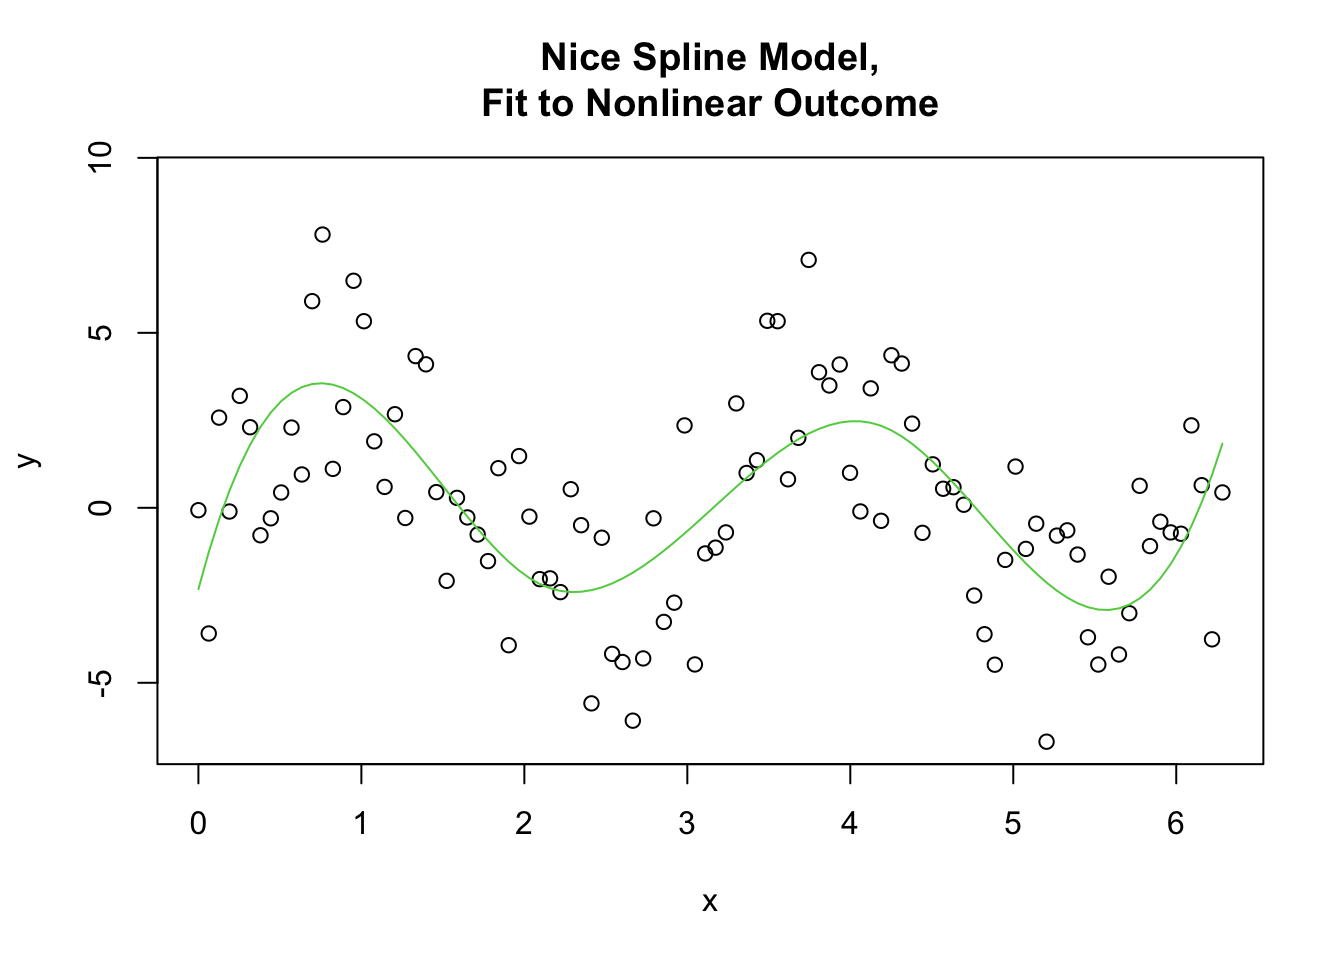
\includegraphics{macro_files/figure-pdf/unnamed-chunk-27-1.pdf}

}

\end{figure}

I really think splines, and GAMs are an excellent addition to the
modeling world and have started teaching them in my own methods courses.
In the world of demography, especially, with age affecting everything,
there is no need to constantly assume relationships are purely linear,
and splines offer an excellent method to explore such relationships.

If these assumptions are violated, then several things can happen. At
best, our interpretation of the model coefficients could be wrong,
meaning that, as seen above, our model would suggest one relationship
from the data, but in fact because the model was misspecified, the
relationship we discover is incorrect. Our poor linear model would
predict a decline in the outcome, while the outcome itself is perfectly
stationary, as shown by the dashed line.

In a more social science sensibility, the interpretation of the beta
coefficients for the effect of \(x\) on \(y\) in this case will provide
us a false conclusion of the relationship in the data. This is a really
dangerous outcome for us in social science, because that's why we're
doing statistics in the first place, to answer questions.

The normality assumption above primarily affect predictions from the
model, which, since the normal distribution is bound on \(-\infty\) to
\(\infty\), can easily lead to a prediction outside of the realm of
possibility, say for a dichotomous outcome, or a count, neither of which
can have predicted values beyond 0 and 1, or less than 0.

\hypertarget{generalized-least-squares}{%
\subsection{Generalized Least Squares}\label{generalized-least-squares}}

Once our data start to violate the assumptions of the linear model, the
model becomes less and less useful. For instance, why make all of the
strict assumptions about homoskedastic (I am contractually required by
the statistics union to say this at least once) variances in the model
residuals in order to use OLS, when you can use it's friend and brother,
\textbf{Generalized Least Squares} (GLS, of course), which allows you to
make useful and pragmatic changes to the OLS model structure to
accommodate all of the fun and annoying things about real data, but
still use the normal distribution to model our
outcomes{[}\^{}macrodem-9{]}.

Generalized Least Squares adds a lot more flexibility to modeling
normally distributed outcomes, basically by allowing us to modify the
fundamental equations above to accommodate unequal variances, or the use
of covariates or stratification variables on variances. Another way to
write the OLS model above would be:

\(\epsilon_i \sim Normal(X'\beta, I\sigma_\epsilon)\) Where \(I\) is the
\textbf{identity matrix}, which implies that for each observation, the
variances in the residuals are all the same:

\[
\sigma_{\epsilon}  = I * \sigma_{\epsilon} = \begin{Bmatrix}
1& 0& 0 \\
0& 1& 0 \\
0& 0& 1\\
\end{Bmatrix} *\sigma_{\epsilon} = \begin{Bmatrix}
\sigma_{\epsilon}& 0& 0 \\
0& \sigma_{\epsilon}& 0 \\
0& 0 & \sigma_{\epsilon} \\
\end{Bmatrix}
\]

Which shows the common variance for the three residuals. GLS allows us
to relax this constant variance assumption, by at the minimum allowing
the variances to be a function of a weighting variable (which produces
\textbf{Weighted Least Squares}), or some covariate. In the most basic
presentation of this principle, this makes the residuals have some
other, non-constant form of:

\(\sigma_{\epsilon} = \Omega\) which in turn modifies the estimation
equation for the \(\beta\)'s to:

\(\beta_{k_{GLS}} = (X' \Omega^{-1} X)^{-1} X' \Omega^{-1} Y\)
Applications of such models are more commonly seen in time series
modeling and longitudinal analysis, where the residuals of the model
often have an autoregressive form to allow individuals to be correlated
with themselves over time, but when talking about place-based
demography, more modifications of the model have been derived that allow
for addressing another key assumption of independence among observations
and nonconstant variances. This in fact is the realm of an entire field
of econometrics, often called \textbf{spatial econometrics} (Anselin
1988; Chi and Zhu 2020; Elhorst 2014; LeSage and Pace 2009).

The \texttt{gls()} function in the \texttt{nlme} library is very
flexible at modeling heteroskedasticity using several types of variance
functions. The general principle of the gls model in terms of modeling
heteroskedasticity is that the OLS model residual variance
\(\sigma_{\epsilon}\) is now not a constant, but a function of
covariates or different variances based on a stratification variable.
This generates a model for the residual variances of the form:

\[Var(\epsilon_i |\beta) = \sigma^2 g\]

Where the \(g\) function can be the effect of a covariate, which would
allow the variance to increase or decrease as function of that variable,
or a set of strata, where the variance can be different in two or more
groups. Below, I first show the model above fit using \texttt{gls()}
instead of \texttt{lm()}, then extend the model to include
heteroskedasticity based on the population size of the county, and
state-specific variance terms (Pinheiro and Bates 2000).

\begin{Shaded}
\begin{Highlighting}[]
\FunctionTok{library}\NormalTok{(nlme)}
\end{Highlighting}
\end{Shaded}

\begin{verbatim}

Attaching package: 'nlme'
\end{verbatim}

\begin{verbatim}
The following object is masked from 'package:dplyr':

    collapse
\end{verbatim}

\begin{Shaded}
\begin{Highlighting}[]
\NormalTok{lm1g}\OtherTok{\textless{}{-}} \FunctionTok{gls}\NormalTok{(lbrate1618 }\SpecialCharTok{\textasciitilde{}}\NormalTok{  fampov14 }\SpecialCharTok{+}\NormalTok{ rucc }\SpecialCharTok{+}\NormalTok{ hpsa16,}
          \AttributeTok{data =}\NormalTok{ ahrf\_m)}

\FunctionTok{summary}\NormalTok{(lm1g)}
\end{Highlighting}
\end{Shaded}

\begin{verbatim}
Generalized least squares fit by REML
  Model: lbrate1618 ~ fampov14 + rucc + hpsa16 
  Data: ahrf_m 
       AIC      BIC    logLik
  19580.52 19655.22 -9777.261

Coefficients:
                                 Value Std.Error  t-value p-value
(Intercept)                   62.26920 1.1890098 52.37063  0.0000
fampov14                       2.25805 0.0684647 32.98129  0.0000
rucc02                        -1.91854 1.2008189 -1.59769  0.1102
rucc03                        -3.38658 1.2505531 -2.70806  0.0068
rucc04                        -6.65483 1.4063909 -4.73185  0.0000
rucc05                        -5.96283 1.9373921 -3.07776  0.0021
rucc06                        -3.94180 1.1431747 -3.44812  0.0006
rucc07                        -4.00730 1.2816639 -3.12664  0.0018
rucc08                         0.45112 2.1106217  0.21374  0.8308
rucc09                        -3.88365 2.2911822 -1.69504  0.0902
hpsa16partial county shortage -0.66219 1.0076706 -0.65715  0.5111
hpsa16whole county shortage    2.36214 1.2533476  1.88466  0.0596

 Correlation: 
                              (Intr) fmpv14 rucc02 rucc03 rucc04 rucc05 rucc06
fampov14                      -0.381                                          
rucc02                        -0.364 -0.121                                   
rucc03                        -0.342 -0.114  0.462                            
rucc04                        -0.298 -0.160  0.416  0.399                     
rucc05                        -0.207 -0.144  0.305  0.293  0.269              
rucc06                        -0.317 -0.245  0.521  0.501  0.453  0.336       
rucc07                        -0.281 -0.242  0.467  0.449  0.410  0.304  0.525
rucc08                        -0.140 -0.163  0.288  0.278  0.248  0.186  0.344
rucc09                        -0.101 -0.226  0.274  0.265  0.241  0.182  0.334
hpsa16partial county shortage -0.560 -0.131 -0.068 -0.078 -0.043 -0.024 -0.070
hpsa16whole county shortage   -0.390 -0.235 -0.035 -0.045  0.017  0.015 -0.105
                              rucc07 rucc08 rucc09 hps16pcs
fampov14                                                   
rucc02                                                     
rucc03                                                     
rucc04                                                     
rucc05                                                     
rucc06                                                     
rucc07                                                     
rucc08                         0.298                       
rucc09                         0.292  0.204                
hpsa16partial county shortage -0.058 -0.051 -0.037         
hpsa16whole county shortage   -0.035 -0.132 -0.097  0.693  

Standardized residuals:
        Min          Q1         Med          Q3         Max 
-5.50851038 -0.63237431 -0.07515361  0.56768444  4.75446234 

Residual standard error: 16.35905 
Degrees of freedom: 2324 total; 2312 residual
\end{verbatim}

These are the same results, in terms of the regression coefficients as
returned by \texttt{lm()}. If we include a \texttt{varFixed()} term, we
can regress the residual variance term on a covariate, in this case I
select the population size.

\begin{Shaded}
\begin{Highlighting}[]
\NormalTok{lm2g}\OtherTok{\textless{}{-}} \FunctionTok{gls}\NormalTok{(lbrate1618 }\SpecialCharTok{\textasciitilde{}}\NormalTok{  fampov14 }\SpecialCharTok{+}\NormalTok{ rucc }\SpecialCharTok{+}\NormalTok{ hpsa16,}
          \AttributeTok{data =}\NormalTok{ ahrf\_m, }
          \AttributeTok{weights =} \FunctionTok{varFixed}\NormalTok{(}\SpecialCharTok{\textasciitilde{}}\NormalTok{popn) )}
\FunctionTok{summary}\NormalTok{(lm2g)}
\end{Highlighting}
\end{Shaded}

\begin{verbatim}
Generalized least squares fit by REML
  Model: lbrate1618 ~ fampov14 + rucc + hpsa16 
  Data: ahrf_m 
       AIC      BIC    logLik
  21560.43 21635.12 -10767.21

Variance function:
 Structure: fixed weights
 Formula: ~popn 

Coefficients:
                                 Value Std.Error  t-value p-value
(Intercept)                   64.51684 1.7992819 35.85700  0.0000
fampov14                       2.02451 0.0672245 30.11574  0.0000
rucc02                        -3.65253 2.0140861 -1.81349  0.0699
rucc03                        -3.74951 1.9836516 -1.89021  0.0589
rucc04                        -6.48571 2.3336913 -2.77916  0.0055
rucc05                        -6.03115 2.9497652 -2.04462  0.0410
rucc06                        -2.53166 1.6616043 -1.52362  0.1277
rucc07                        -2.30731 1.7300102 -1.33369  0.1824
rucc08                         0.54783 2.1293518  0.25727  0.7970
rucc09                        -2.85405 2.1820264 -1.30798  0.1910
hpsa16partial county shortage  0.18574 1.3009964  0.14277  0.8865
hpsa16whole county shortage    5.22180 1.4198726  3.67766  0.0002

 Correlation: 
                              (Intr) fmpv14 rucc02 rucc03 rucc04 rucc05 rucc06
fampov14                      -0.269                                          
rucc02                        -0.537 -0.065                                   
rucc03                        -0.550 -0.045  0.536                            
rucc04                        -0.466 -0.088  0.463  0.466                     
rucc05                        -0.363 -0.085  0.367  0.370  0.328              
rucc06                        -0.603 -0.163  0.649  0.655  0.568  0.452       
rucc07                        -0.591 -0.169  0.627  0.631  0.555  0.441  0.776
rucc08                        -0.431 -0.174  0.508  0.513  0.439  0.350  0.637
rucc09                        -0.409 -0.234  0.500  0.503  0.435  0.348  0.632
hpsa16partial county shortage -0.464 -0.092 -0.062 -0.062 -0.063 -0.048 -0.109
hpsa16whole county shortage   -0.429 -0.215 -0.016 -0.027  0.038  0.031 -0.050
                              rucc07 rucc08 rucc09 hps16pcs
fampov14                                                   
rucc02                                                     
rucc03                                                     
rucc04                                                     
rucc05                                                     
rucc06                                                     
rucc07                                                     
rucc08                         0.609                       
rucc09                         0.605  0.512                
hpsa16partial county shortage -0.100 -0.101 -0.087         
hpsa16whole county shortage    0.001 -0.099 -0.070  0.767  

Standardized residuals:
        Min          Q1         Med          Q3         Max 
-7.55351050 -0.48060084 -0.06047952  0.31143188  8.68535299 

Residual standard error: 0.1103656 
Degrees of freedom: 2324 total; 2312 residual
\end{verbatim}

This model shows some very different effects after controlling for
non-constant variance. For instance, the
\texttt{whole\ county\ shortage} effect is now much more significant in
the model, compared to the \texttt{lm1} model.

The final model includes a separate variance for each state using the
\texttt{varIdent()} term.

\begin{Shaded}
\begin{Highlighting}[]
\NormalTok{lm3}\OtherTok{\textless{}{-}} \FunctionTok{gls}\NormalTok{(lbrate1618 }\SpecialCharTok{\textasciitilde{}}\NormalTok{  fampov14 }\SpecialCharTok{+}\NormalTok{ rucc }\SpecialCharTok{+}\NormalTok{ hpsa16,}
          \AttributeTok{data =}\NormalTok{ ahrf\_m, }
          \AttributeTok{weights =} \FunctionTok{varIdent}\NormalTok{(}\AttributeTok{form =} \SpecialCharTok{\textasciitilde{}}\DecValTok{1}\SpecialCharTok{|}\FunctionTok{factor}\NormalTok{(state) ) )}
\FunctionTok{summary}\NormalTok{(lm3)}
\end{Highlighting}
\end{Shaded}

\begin{verbatim}
Generalized least squares fit by REML
  Model: lbrate1618 ~ fampov14 + rucc + hpsa16 
  Data: ahrf_m 
       AIC      BIC    logLik
  19232.57 19583.07 -9555.287

Variance function:
 Structure: Different standard deviations per stratum
 Formula: ~1 | factor(state) 
 Parameter estimates:
       21        01        04        05        06        08        09        11 
1.0000000 1.6653572 1.4666877 1.3444082 1.4169906 2.3439093 0.4153761 0.9349384 
       12        13        16        17        18        48        49        50 
0.8691605 1.4618211 1.2492319 0.8531463 0.7272325 1.0046612 0.9955712 0.6782617 
       22        23        24        25        26        27        28        29 
1.5206083 0.5562842 1.0764207 0.3632039 0.8797361 0.8694446 2.1388815 1.0671070 
       30        33        34        35        36        37        38        39 
0.8593438 0.3518410 0.5857512 1.6675040 0.8834383 1.2756652 1.3451314 0.7590721 
       40        41        42        44        45        46        47        51 
0.9096844 0.9789355 0.7160118 0.7725377 1.4955639 2.2706999 0.9232718 1.4150226 
       53        54        55        10        32        19        20        56 
1.1651279 1.4044153 0.8102840 0.8493449 1.3739156 0.8028595 0.9380637 1.5713111 
       31 
1.1601422 

Coefficients:
                                 Value Std.Error  t-value p-value
(Intercept)                   61.00371 0.9636746 63.30323  0.0000
fampov14                       2.20339 0.0626079 35.19354  0.0000
rucc02                        -1.55250 0.9300585 -1.66925  0.0952
rucc03                        -2.67599 0.9989933 -2.67869  0.0074
rucc04                        -6.75071 1.0541928 -6.40368  0.0000
rucc05                        -7.07431 1.6290634 -4.34256  0.0000
rucc06                        -5.33031 0.8964666 -5.94591  0.0000
rucc07                        -6.20026 1.0294913 -6.02264  0.0000
rucc08                        -0.38337 1.8548174 -0.20669  0.8363
rucc09                        -3.80880 2.0564547 -1.85212  0.0641
hpsa16partial county shortage -0.40513 0.8049182 -0.50332  0.6148
hpsa16whole county shortage    0.69954 1.0571871  0.66170  0.5082

 Correlation: 
                              (Intr) fmpv14 rucc02 rucc03 rucc04 rucc05 rucc06
fampov14                      -0.425                                          
rucc02                        -0.330 -0.118                                   
rucc03                        -0.300 -0.112  0.415                            
rucc04                        -0.281 -0.137  0.396  0.369                     
rucc05                        -0.155 -0.132  0.262  0.244  0.236              
rucc06                        -0.275 -0.238  0.476  0.446  0.423  0.284       
rucc07                        -0.232 -0.230  0.417  0.390  0.374  0.253  0.467
rucc08                        -0.105 -0.142  0.235  0.221  0.207  0.140  0.280
rucc09                        -0.058 -0.215  0.222  0.209  0.199  0.138  0.272
hpsa16partial county shortage -0.592 -0.112 -0.037 -0.042 -0.028 -0.026 -0.037
hpsa16whole county shortage   -0.390 -0.189 -0.015 -0.026  0.019  0.016 -0.106
                              rucc07 rucc08 rucc09 hps16pcs
fampov14                                                   
rucc02                                                     
rucc03                                                     
rucc04                                                     
rucc05                                                     
rucc06                                                     
rucc07                                                     
rucc08                         0.236                       
rucc09                         0.233  0.147                
hpsa16partial county shortage -0.036 -0.032 -0.019         
hpsa16whole county shortage   -0.031 -0.110 -0.076  0.654  

Standardized residuals:
        Min          Q1         Med          Q3         Max 
-3.71110304 -0.57404142  0.07995833  0.73280651  3.80484317 

Residual standard error: 13.75474 
Degrees of freedom: 2324 total; 2312 residual
\end{verbatim}

Which also provides similar results to \texttt{lm1}. So, which model is
better for this particular outcome? One way to examine relative model
fit is to compare the Akaike Information Criteria (AIC) for the three
models. The AIC consists of two components, one showing overall model
deviance, or residual variance and a penalty term for the number of
parameters in a model. A general form of it is:

\[
AIC = -2LL(\theta) + 2k
\] Where the term \(-2LL(\theta)\) is the model -2 Log likelihood, or
\emph{deviance}, and \(2k\) is a penalty term with \(k\) being the
number of parameters.

Since the three models \texttt{lm1g}, \texttt{lm2} and \texttt{lm3} are
all fit by \texttt{gls()}, and fit to the same dataset, we can compare
them. We can even add another model with a smooth spline effect of
poverty:

\begin{Shaded}
\begin{Highlighting}[]
\NormalTok{lm3s}\OtherTok{\textless{}{-}} \FunctionTok{gls}\NormalTok{(lbrate1618 }\SpecialCharTok{\textasciitilde{}}  \FunctionTok{bs}\NormalTok{(fampov14, }\AttributeTok{df=}\DecValTok{4}\NormalTok{) }\SpecialCharTok{+}\NormalTok{ rucc }\SpecialCharTok{+}\NormalTok{ hpsa16,}
          \AttributeTok{data =}\NormalTok{ ahrf\_m, }
          \AttributeTok{weights =} \FunctionTok{varIdent}\NormalTok{(}\AttributeTok{form =} \SpecialCharTok{\textasciitilde{}}\DecValTok{1}\SpecialCharTok{|}\FunctionTok{factor}\NormalTok{(state) ) )}
\FunctionTok{summary}\NormalTok{(lm3s)}
\end{Highlighting}
\end{Shaded}

\begin{verbatim}
Generalized least squares fit by REML
  Model: lbrate1618 ~ bs(fampov14, df = 4) + rucc + hpsa16 
  Data: ahrf_m 
       AIC      BIC    logLik
  19166.97 19534.62 -9519.486

Variance function:
 Structure: Different standard deviations per stratum
 Formula: ~1 | factor(state) 
 Parameter estimates:
       21        01        04        05        06        08        09        11 
1.0000000 1.8015440 1.5283795 1.4399605 1.5393732 2.5102463 0.4584789 0.8961499 
       12        13        16        17        18        48        49        50 
0.9169369 1.5786894 1.2845194 0.9010857 0.7815679 1.0169676 1.0666628 0.7347100 
       22        23        24        25        26        27        28        29 
1.7020601 0.6180479 1.1587213 0.4065278 0.9556412 0.9113779 2.4411415 1.1501547 
       30        33        34        35        36        37        38        39 
0.9098260 0.3629158 0.6330773 1.6758907 0.9583268 1.3320870 1.3647418 0.8178477 
       40        41        42        44        45        46        47        51 
0.9867867 1.0609522 0.7586694 0.8150356 1.5564278 1.0001279 0.9815430 1.5006645 
       53        54        55        10        32        19        20        56 
1.2497825 1.4843275 0.8554764 0.9154187 1.4561259 0.8426759 1.0163896 1.7112344 
       31 
1.2457365 

Coefficients:
                                 Value Std.Error   t-value p-value
(Intercept)                   65.28605  2.227553 29.308421  0.0000
bs(fampov14, df = 4)1          4.58369  3.031480  1.512031  0.1307
bs(fampov14, df = 4)2         50.98375  3.137696 16.248784  0.0000
bs(fampov14, df = 4)3         72.74204  8.455071  8.603362  0.0000
bs(fampov14, df = 4)4         15.96517 11.310702  1.411510  0.1582
rucc02                        -1.78937  0.947673 -1.888176  0.0591
rucc03                        -2.99112  1.007407 -2.969130  0.0030
rucc04                        -6.96833  1.065192 -6.541851  0.0000
rucc05                        -7.95180  1.605224 -4.953700  0.0000
rucc06                        -5.72170  0.906461 -6.312131  0.0000
rucc07                        -6.38566  1.028234 -6.210321  0.0000
rucc08                        -0.84020  1.849541 -0.454273  0.6497
rucc09                        -3.84206  2.006058 -1.915231  0.0556
hpsa16partial county shortage -0.54729  0.798950 -0.685016  0.4934
hpsa16whole county shortage    0.60030  1.043145  0.575469  0.5650

 Correlation: 
                              (Intr) b(14,d=4)1 b(14,d=4)2 b(14,d=4)3
bs(fampov14, df = 4)1         -0.907                                 
bs(fampov14, df = 4)2         -0.157 -0.005                          
bs(fampov14, df = 4)3         -0.527  0.664     -0.533               
bs(fampov14, df = 4)4         -0.089  0.053      0.318     -0.304    
rucc02                         0.011 -0.166     -0.133     -0.073    
rucc03                        -0.008 -0.129     -0.146     -0.034    
rucc04                        -0.002 -0.132     -0.134     -0.060    
rucc05                         0.006 -0.088     -0.128     -0.034    
rucc06                         0.001 -0.142     -0.190     -0.081    
rucc07                        -0.011 -0.120     -0.139     -0.100    
rucc08                        -0.015 -0.040     -0.115     -0.019    
rucc09                         0.006 -0.063     -0.076     -0.095    
hpsa16partial county shortage -0.166 -0.091     -0.123     -0.029    
hpsa16whole county shortage   -0.143 -0.042     -0.096     -0.055    
                              b(14,d=4)4 rucc02 rucc03 rucc04 rucc05 rucc06
bs(fampov14, df = 4)1                                                      
bs(fampov14, df = 4)2                                                      
bs(fampov14, df = 4)3                                                      
bs(fampov14, df = 4)4                                                      
rucc02                        -0.036                                       
rucc03                        -0.038      0.435                            
rucc04                        -0.035      0.414  0.388                     
rucc05                        -0.032      0.282  0.265  0.255              
rucc06                        -0.043      0.495  0.466  0.441  0.304       
rucc07                        -0.035      0.433  0.406  0.390  0.269  0.482
rucc08                        -0.019      0.243  0.231  0.216  0.150  0.290
rucc09                        -0.114      0.231  0.216  0.207  0.146  0.283
hpsa16partial county shortage -0.031     -0.012 -0.023 -0.009 -0.003 -0.013
hpsa16whole county shortage   -0.054     -0.006 -0.019  0.026  0.027 -0.096
                              rucc07 rucc08 rucc09 hps16pcs
bs(fampov14, df = 4)1                                      
bs(fampov14, df = 4)2                                      
bs(fampov14, df = 4)3                                      
bs(fampov14, df = 4)4                                      
rucc02                                                     
rucc03                                                     
rucc04                                                     
rucc05                                                     
rucc06                                                     
rucc07                                                     
rucc08                         0.243                       
rucc09                         0.245  0.152                
hpsa16partial county shortage -0.015 -0.022 -0.015         
hpsa16whole county shortage   -0.018 -0.107 -0.073  0.650  

Standardized residuals:
        Min          Q1         Med          Q3         Max 
-3.66477973 -0.58141552  0.08014607  0.72668723  3.87024262 

Residual standard error: 12.88614 
Degrees of freedom: 2324 total; 2309 residual
\end{verbatim}

\begin{Shaded}
\begin{Highlighting}[]
\FunctionTok{AIC}\NormalTok{( lm1g,  lm2g, lm3, lm3s)}
\end{Highlighting}
\end{Shaded}

\begin{verbatim}
Warning in AIC.default(lm1g, lm2g, lm3, lm3s): models are not all fitted to the
same number of observations
\end{verbatim}

\begin{verbatim}
     df      AIC
lm1g 13 19580.52
lm2g 13 21560.43
lm3  61 19232.57
lm3s 64 19166.97
\end{verbatim}

The \texttt{AIC()} function calculates AIC for each model, and we see
that \texttt{lm3s} has the lowest of the three, suggesting that the
non-constant variance across states is a better representation than the
effects of population size on the residual variance, and that the
nonlinear effect of poverty is also present in this case.

\hypertarget{further-model-comparisons}{%
\subsubsection{Further model
comparisons}\label{further-model-comparisons}}

R has a general method of comparing models using \(F\) tests or
Likelihood Ratio Tests. These are often used when comparing nested
models, where one model is a simplified version of another. We have such
models above in our \texttt{gls()} models. The \texttt{lm1g} model is a
simplified version of the \texttt{lm3} model because it doesn't contain
the extra parameters modeling the unequal variances. The
\texttt{anova()} method can compare the models to see if the extra
parameters are explaining the model deviance (or variation) better.

\begin{Shaded}
\begin{Highlighting}[]
\FunctionTok{anova}\NormalTok{(lm1g, lm3)}
\end{Highlighting}
\end{Shaded}

\begin{verbatim}
     Model df      AIC      BIC    logLik   Test  L.Ratio p-value
lm1g     1 13 19580.52 19655.22 -9777.261                        
lm3      2 61 19232.57 19583.07 -9555.287 1 vs 2 443.9476  <.0001
\end{verbatim}

Here the likelihood ratio test \texttt{L.Ratio} shows a significant
decrease in the \texttt{logLik} in model \texttt{lm3}, suggesting that
it better explains the data than \texttt{lm1g} does. The likelihood
ratio is calculated as \(2*LL_2 - LL_1\), or in the case above
\texttt{2*(-9555.287-\/-9777.261)}. The \texttt{anova} method is very
useful for comparing alternative models and can be used on most of the
models shown in this book.

\hypertarget{predictions-and-marginal-means}{%
\subsection{Predictions and marginal
means}\label{predictions-and-marginal-means}}

Working with fitted values from a regression is one of the least taught
aspects of modeling. Since the models are fundamentally doing very fancy
averaging, the estimated, or fitted values from the model can often be
very useful to us as we try to explain the results of our models.
Remember, the fitted values of the model are just:

\[
\hat{y}_i = \sum \hat{\beta_k} x_{ki}
\]

or the linear combination of the estimated model parameters and the
\(k\) observed predictors, \(x_{ki}\). Most models in R have a
\texttt{fitted()} method to extract the fitted values of the outcome
variable for each observation.

For example, here are the first six fitted values from the original
\texttt{lm1} OLS model, the \texttt{gls()} heteroskedastic model
\texttt{lm3} model, and the first six values of the outcome:

\begin{Shaded}
\begin{Highlighting}[]
\FunctionTok{library}\NormalTok{(gt)}

\NormalTok{fits}\OtherTok{\textless{}{-}} \FunctionTok{data.frame}\NormalTok{(}
  \AttributeTok{name =} \FunctionTok{head}\NormalTok{( ahrf\_m}\SpecialCharTok{$}\NormalTok{NAME ),}
  \AttributeTok{lm1 =} \FunctionTok{head}\NormalTok{( }\FunctionTok{fitted}\NormalTok{ ( lm1 )),}
  \AttributeTok{lm3 =} \FunctionTok{head}\NormalTok{( }\FunctionTok{fitted}\NormalTok{( lm3 )), }
  \AttributeTok{observed =} \FunctionTok{head}\NormalTok{( ahrf\_m}\SpecialCharTok{$}\NormalTok{lbrate1618 )}
\NormalTok{  )}

\NormalTok{fits}\SpecialCharTok{\%\textgreater{}\%}
  \FunctionTok{gt}\NormalTok{()}
\end{Highlighting}
\end{Shaded}

\begin{longtable*}{lrrr}
\toprule
name & lm1 & lm3 & observed \\ 
\midrule
Anderson & 83.16599 & 79.91074 & 87.78626 \\ 
Bullitt & 79.44563 & 78.00540 & 84.47205 \\ 
Clark & 85.43028 & 84.16478 & 89.20188 \\ 
Daviess & 86.20507 & 84.98880 & 81.26411 \\ 
Hardin & 82.15580 & 81.27857 & 78.47222 \\ 
Harrison & 83.16599 & 79.91074 & 81.89655 \\ 
\bottomrule
\end{longtable*}

We can also easily construct the map of the observed, fitted values and
residuals from the model using \texttt{tmap}.

\begin{Shaded}
\begin{Highlighting}[]
\NormalTok{ahrf\_m}\SpecialCharTok{$}\NormalTok{fitted\_lm3 }\OtherTok{\textless{}{-}} \FunctionTok{predict}\NormalTok{(lm3)}

\NormalTok{ahrf\_m}\SpecialCharTok{$}\NormalTok{resid }\OtherTok{\textless{}{-}} \FunctionTok{resid}\NormalTok{(lm3)}

\NormalTok{actual }\OtherTok{\textless{}{-}}\FunctionTok{tm\_shape}\NormalTok{(ahrf\_m)}\SpecialCharTok{+}
  \FunctionTok{tm\_polygons}\NormalTok{(}\StringTok{"lbrate1618"}\NormalTok{,}
              \AttributeTok{palette =} \StringTok{"Blues"}\NormalTok{,}
              \AttributeTok{n=}\DecValTok{6}\NormalTok{,}
              \AttributeTok{style=}\StringTok{"fisher"}\NormalTok{,}
              \AttributeTok{border.col =} \ConstantTok{NULL}\NormalTok{,}
              \AttributeTok{colorNA =} \StringTok{"grey50"}\NormalTok{)}\SpecialCharTok{+}
  \FunctionTok{tm\_shape}\NormalTok{(sts)}\SpecialCharTok{+}
  \FunctionTok{tm\_lines}\NormalTok{( }\AttributeTok{col =} \StringTok{"black"}\NormalTok{)}

\NormalTok{fit}\OtherTok{\textless{}{-}}\FunctionTok{tm\_shape}\NormalTok{(ahrf\_m)}\SpecialCharTok{+}
  \FunctionTok{tm\_polygons}\NormalTok{(}\StringTok{"fitted\_lm3"}\NormalTok{,}
              \AttributeTok{palette =} \StringTok{"Blues"}\NormalTok{,}
              \AttributeTok{n=}\DecValTok{6}\NormalTok{,}
              \AttributeTok{style=}\StringTok{"fisher"}\NormalTok{, }
              \AttributeTok{border.col =} \ConstantTok{NULL}\NormalTok{,}
              \AttributeTok{colorNA =} \StringTok{"grey50"}\NormalTok{)}\SpecialCharTok{+}
  \FunctionTok{tm\_shape}\NormalTok{(sts)}\SpecialCharTok{+}
  \FunctionTok{tm\_lines}\NormalTok{( }\AttributeTok{col =} \StringTok{"black"}\NormalTok{)}

\NormalTok{resids}\OtherTok{\textless{}{-}}\FunctionTok{tm\_shape}\NormalTok{(ahrf\_m)}\SpecialCharTok{+}
  \FunctionTok{tm\_polygons}\NormalTok{(}\StringTok{"resid"}\NormalTok{,}
              \AttributeTok{palette =} \StringTok{"RdBu"}\NormalTok{,}
              \AttributeTok{n=}\DecValTok{6}\NormalTok{,}
              \AttributeTok{style=}\StringTok{"fisher"}\NormalTok{,}
              \AttributeTok{midpoint =} \ConstantTok{NA}\NormalTok{,}
              \AttributeTok{border.col =} \ConstantTok{NULL}\NormalTok{,}
              \AttributeTok{colorNA =} \StringTok{"grey50"}\NormalTok{)}\SpecialCharTok{+}
  \FunctionTok{tm\_shape}\NormalTok{(sts)}\SpecialCharTok{+}
  \FunctionTok{tm\_lines}\NormalTok{( }\AttributeTok{col =} \StringTok{"black"}\NormalTok{)}


\FunctionTok{tmap\_arrange}\NormalTok{(actual, fit, resids, }\AttributeTok{nrow=}\DecValTok{2}\NormalTok{)}
\end{Highlighting}
\end{Shaded}

\begin{figure}[H]

{\centering \includegraphics{macro_files/figure-pdf/unnamed-chunk-35-1.pdf}

}

\end{figure}

This map layout shows the observed rates, the fitted rates from the
\texttt{lm3} model and the residuals from the model. Mapping residuals
from models run on place-based data can show areas within the data where
the model is consistently under or over-estimating the outcome. For
instance in the example above, we see consistently high residuals in
several of the south eastern states, and the mountain west, and several
areas where the residuals are consistently negative, meaning we are
over-estimating the rate. This can be instructive as to other variables
we may be leaving out of the model that follow similar spatial
distributions of the residuals. If such spatially patterned residuals
are observed, it is generally a good idea to consider a statistical
model that incorporates some kind of spatially explicit model
specification.

\hypertarget{more-on-predicted-values}{%
\subsubsection{More on predicted
values}\label{more-on-predicted-values}}

There are more systematic methods for generating predictions from a
model that allow us to marginalize the estimates across other variables
and to generate counter factual or hypothetical rates using combinations
of \(x\) values that may not be observed in the data. The
\texttt{emmeans} package is very good at this and also accommodates many
types of models. For instance if we would like the marginal means for
counties by their healthcare shortage area type, after controlling for
the other variables in our model, we can request that.

\begin{Shaded}
\begin{Highlighting}[]
\FunctionTok{library}\NormalTok{(emmeans)}
\NormalTok{rg}\OtherTok{\textless{}{-}} \FunctionTok{ref\_grid}\NormalTok{(lm3s)}

\NormalTok{mu1 }\OtherTok{\textless{}{-}} \FunctionTok{emmeans}\NormalTok{(rg, }\AttributeTok{specs =}\StringTok{"hpsa16"}\NormalTok{ )}
\NormalTok{mu1}\SpecialCharTok{\%\textgreater{}\%}
  \FunctionTok{as.data.frame}\NormalTok{()}\SpecialCharTok{\%\textgreater{}\%}
  \FunctionTok{gt}\NormalTok{()}
\end{Highlighting}
\end{Shaded}

\begin{longtable*}{crrrrr}
\toprule
hpsa16 & emmean & SE & df & lower.CL & upper.CL \\ 
\midrule
no shortage & 83.82779 & 0.8441041 & 2261 & 82.17249 & 85.48309 \\ 
partial county shortage & 83.28049 & 0.4890943 & 2261 & 82.32137 & 84.23962 \\ 
whole county shortage & 84.42809 & 0.7923959 & 2261 & 82.87419 & 85.98198 \\ 
\bottomrule
\end{longtable*}

Which unsurprisingly does not tell us much, because the health care
shortage area variable in \texttt{lm3} was not a significant predictor
of the low birth weight rate. We can include more than one margin in the
function, and include specific values we wish to highlight. For
instance, let's compare three hypothetical counties with three different
poverty rates, we can use the \texttt{summary(ahrf\_m\$fampov14)} to see
the first and third quartiles of the distribution and the mean, we will
use these as our theoretical values.

\begin{Shaded}
\begin{Highlighting}[]
\NormalTok{rg}\OtherTok{\textless{}{-}}\FunctionTok{ref\_grid}\NormalTok{(lm3,}
             \AttributeTok{at=}\FunctionTok{list}\NormalTok{( }\AttributeTok{fampov14 =} \FunctionTok{c}\NormalTok{(}\FloatTok{1.8}\NormalTok{,}\FloatTok{7.8}\NormalTok{, }\FloatTok{11.6}\NormalTok{, }\FloatTok{14.3}\NormalTok{, }\FloatTok{52.1}\NormalTok{) ) )}

\NormalTok{means }\OtherTok{\textless{}{-}} \FunctionTok{emmeans}\NormalTok{(rg, }\AttributeTok{specs =} \FunctionTok{c}\NormalTok{(}\StringTok{"fampov14"}\NormalTok{, }\StringTok{"rucc"}\NormalTok{))}

\NormalTok{means}\SpecialCharTok{\%\textgreater{}\%}
  \FunctionTok{as.data.frame}\NormalTok{()}\SpecialCharTok{\%\textgreater{}\%}
  \FunctionTok{ggplot}\NormalTok{(}\FunctionTok{aes}\NormalTok{(}\AttributeTok{x=}\NormalTok{rucc, }\AttributeTok{y=}\NormalTok{emmean))}\SpecialCharTok{+}
  \FunctionTok{geom\_line}\NormalTok{(}\FunctionTok{aes}\NormalTok{(}\AttributeTok{group=}\FunctionTok{factor}\NormalTok{(fampov14), }\AttributeTok{color=}\FunctionTok{factor}\NormalTok{(fampov14)))}\SpecialCharTok{+}
  \FunctionTok{theme\_classic}\NormalTok{()}
\end{Highlighting}
\end{Shaded}

\begin{figure}[H]

{\centering 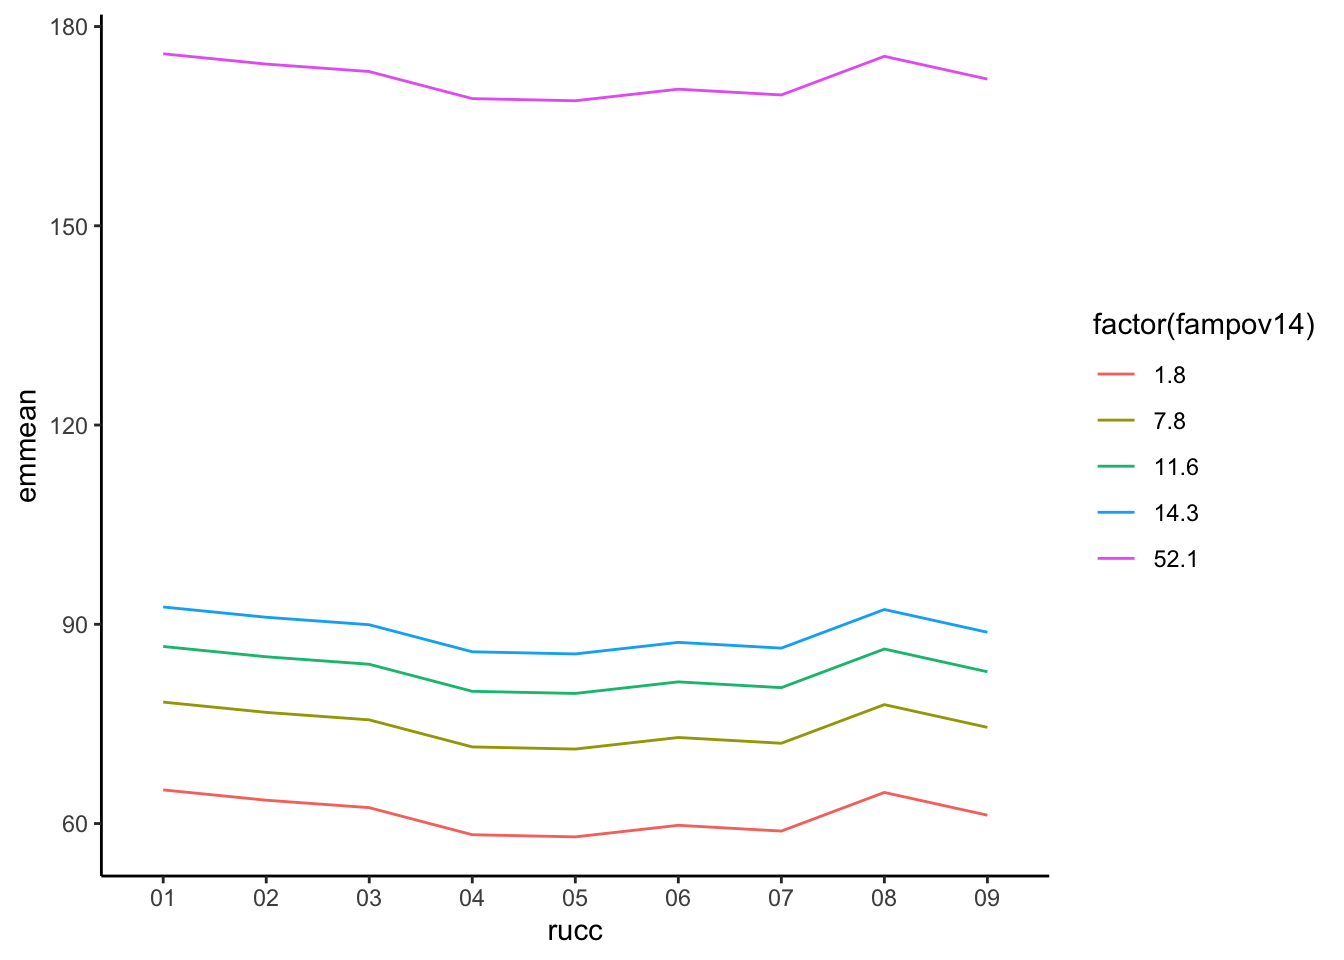
\includegraphics{macro_files/figure-pdf/unnamed-chunk-37-1.pdf}

}

\end{figure}

Which illustrates the differences in the poverty rates on the low birth
weight rate across the rural-urban continuum. The use of these marginal
means is very useful when illustrating the effects of covariates in
regression models, and to effectively illustrate interactions in such
models. For instance, if we estimate the model below, which interacts
the poverty rate with the rural-urban continuum code:

\begin{Shaded}
\begin{Highlighting}[]
\NormalTok{lm3i}\OtherTok{\textless{}{-}} \FunctionTok{gls}\NormalTok{(lbrate1618 }\SpecialCharTok{\textasciitilde{}}\NormalTok{  fampov14 }\SpecialCharTok{*}\NormalTok{ rucc }\SpecialCharTok{+}\NormalTok{ hpsa16,}
          \AttributeTok{data =}\NormalTok{ ahrf\_m, }
          \AttributeTok{weights =} \FunctionTok{varIdent}\NormalTok{(}\AttributeTok{form =} \SpecialCharTok{\textasciitilde{}}\DecValTok{1}\SpecialCharTok{|}\FunctionTok{factor}\NormalTok{(state) ) )}
\end{Highlighting}
\end{Shaded}

\begin{Shaded}
\begin{Highlighting}[]
\NormalTok{rg}\OtherTok{\textless{}{-}}\FunctionTok{ref\_grid}\NormalTok{(lm3i,}
             \AttributeTok{at=}\FunctionTok{list}\NormalTok{( }\AttributeTok{fampov14 =} \FunctionTok{c}\NormalTok{(}\FloatTok{7.8}\NormalTok{, }\FloatTok{11.6}\NormalTok{, }\FloatTok{14.3}\NormalTok{) ) )}

\NormalTok{means }\OtherTok{\textless{}{-}} \FunctionTok{emmeans}\NormalTok{(rg, }\AttributeTok{specs =} \FunctionTok{c}\NormalTok{(}\StringTok{"fampov14"}\NormalTok{, }\StringTok{"rucc"}\NormalTok{))}

\NormalTok{means}\SpecialCharTok{\%\textgreater{}\%}
  \FunctionTok{as.data.frame}\NormalTok{()}\SpecialCharTok{\%\textgreater{}\%}
  \FunctionTok{ggplot}\NormalTok{(}\FunctionTok{aes}\NormalTok{(}\AttributeTok{x=}\NormalTok{rucc, }\AttributeTok{y=}\NormalTok{emmean))}\SpecialCharTok{+}
  \FunctionTok{geom\_line}\NormalTok{(}\FunctionTok{aes}\NormalTok{(}\AttributeTok{group=}\FunctionTok{factor}\NormalTok{(fampov14), }\AttributeTok{color=}\FunctionTok{factor}\NormalTok{(fampov14)))}\SpecialCharTok{+}
  \FunctionTok{theme\_classic}\NormalTok{()}
\end{Highlighting}
\end{Shaded}

\begin{figure}[H]

{\centering 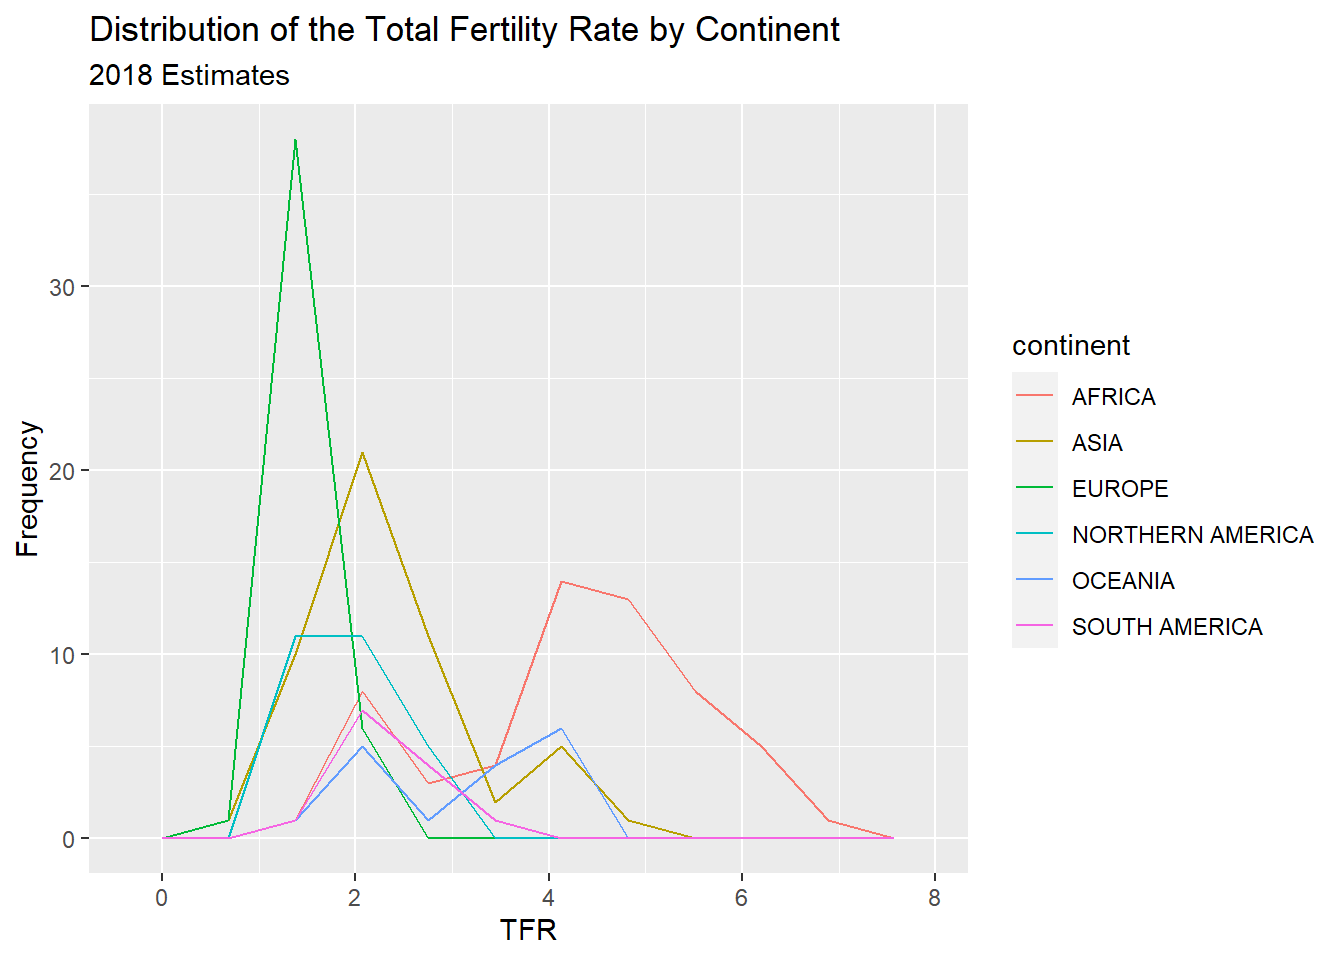
\includegraphics{macro_files/figure-pdf/unnamed-chunk-39-1.pdf}

}

\end{figure}

We can see that in the most rural areas, (the \texttt{09} level of
\texttt{rucc}), the differences by poverty rate are less than in more
metropolitan areas, such as the \texttt{02} or \texttt{03} levels.

\hypertarget{use-of-ols-for-place-based-models}{%
\subsubsection{Use of OLS for place-based
models}\label{use-of-ols-for-place-based-models}}

The OLS model and its extensions are a very useful staring place when
analyzing data on places. For nothing more than the interpretive ease of
the models estimates, it presents a very attractive choice for
ecological modeling. The extension of the model through weighted and
generalized least square allows for more flexible modeling to
accommodate non-constant variance that often arises. Further extensions
of the model by techniques of spatial econometrics further allow for
direct incorporation of spatially correlated and lagged effects of
covariates and model error terms to better deal with the idiosyncrasies
of place-based data (Chi and Zhu 2020; Elhorst 2014; LeSage and Pace
2009). These methods have seen wide use in demographic research over the
past twenty years. Despite the fundamental flexibility of the OLS model,
it may still not present the best solution when modeling demographic
rates. One glaring reason is that if our outcomes are measured as rates,
which are effectively probabilities, then the model can easily lead to
estimates of predicted values that are either negative or greater than
one, either of which presenting an issue for limited outcomes. In fact,
this is why I am a strong proponent of not using the linear model for
estimating probabilities. The next section of the book turns to the use
of the \emph{Generalized Linear Model} (Nelder and Wedderburn 1972;
McCullagh and Nelder 1998) as an alternative modeling strategy,
especially when considering place-based data, when data are measured
either as rates or as relative risks.

\newpage

\hypertarget{basics-of-generalized-linear-models}{%
\section{Basics of Generalized Linear
Models}\label{basics-of-generalized-linear-models}}

Up until now, we have been relying on linear statistical models which
assumed the Normal distribution for our outcomes. A broader class of
regression models, are \textbf{\emph{Generalized Linear Models}} (Nelder
and Wedderburn 1972; McCullagh and Nelder 1998), or \textbf{GLM}s, which
allow for the estimation of a linear regression specification for
outcomes that are not assumed to come from a Normal distribution. GLMs
are a class of statistical models with three underlying components: A
probability density appropriate to the outcome, a link function and a
linear predictor. The \textbf{\emph{link function}} is some mathematical
function that links the mean of the specified probability distribution
to the linear predictor of regression parameters and covariates. For
example, the Normal distribution used by the OLS model has the mean,
\(\mu\), which is typically estimated using the \textbf{\emph{linear
mean function}} : \(\mu = \beta_0 + \beta_1 x_1\) Which describes the
line that estimates the mean of the outcome variable as a linear
function of \(\beta\) parameters and the predictor variable \(x_1\). The
OLS, or \emph{Gaussian} GLM model uses an \textbf{\emph{identity link}}
meaning there is no transformation of the linear mean function as it is
connected to the mean of the outcome. This can be written as:

\[g(u) = g(E(Y)) = \beta_0 + \beta_1 x_1\]

Where \(g()\) is the link function, linking the mean of the Normal
distribution to the linear mean function of the model. The equivalent
GLM model to the \texttt{lm1} model from the previous section is:

\begin{Shaded}
\begin{Highlighting}[]
\NormalTok{glm1}\OtherTok{\textless{}{-}} \FunctionTok{glm}\NormalTok{(lbrate1618 }\SpecialCharTok{\textasciitilde{}}\NormalTok{  fampov14 }\SpecialCharTok{+}\NormalTok{ rucc }\SpecialCharTok{+}\NormalTok{ hpsa16,}
          \AttributeTok{data =}\NormalTok{ ahrf\_m, }
          \AttributeTok{family =}\NormalTok{gaussian)}
\FunctionTok{library}\NormalTok{(texreg)}
\end{Highlighting}
\end{Shaded}

\begin{verbatim}
Version:  1.38.6
Date:     2022-04-06
Author:   Philip Leifeld (University of Essex)

Consider submitting praise using the praise or praise_interactive functions.
Please cite the JSS article in your publications -- see citation("texreg").
\end{verbatim}

\begin{verbatim}

Attaching package: 'texreg'
\end{verbatim}

\begin{verbatim}
The following object is masked from 'package:tidyr':

    extract
\end{verbatim}

\begin{Shaded}
\begin{Highlighting}[]
\FunctionTok{texreg}\NormalTok{(}\FunctionTok{list}\NormalTok{(glm1, lm1), }\AttributeTok{file =} \StringTok{"4\_1.tex"}\NormalTok{)}
\end{Highlighting}
\end{Shaded}

\begin{verbatim}
The table was written to the file '4_1.tex'.
\end{verbatim}

\begin{Shaded}
\begin{Highlighting}[]
\NormalTok{lm1\_t}\OtherTok{\textless{}{-}}\NormalTok{lm1}\SpecialCharTok{\%\textgreater{}\%}
  \FunctionTok{tbl\_regression}\NormalTok{()}



\NormalTok{glm1\_t}\OtherTok{\textless{}{-}}\NormalTok{glm1}\SpecialCharTok{\%\textgreater{}\%}
  \FunctionTok{tbl\_regression}\NormalTok{()}
 

\NormalTok{t\_m }\OtherTok{\textless{}{-}} \FunctionTok{tbl\_merge}\NormalTok{(}
    \AttributeTok{tbls =} \FunctionTok{list}\NormalTok{(lm1\_t, glm1\_t),}
    \AttributeTok{tab\_spanner =} \FunctionTok{c}\NormalTok{(}\StringTok{"**OLS**"}\NormalTok{, }\StringTok{"**GLM**"}\NormalTok{)}
\NormalTok{  ) }

\NormalTok{t\_m}
\end{Highlighting}
\end{Shaded}

\begin{verbatim}
Table printed with `knitr::kable()`, not {gt}. Learn why at
https://www.danieldsjoberg.com/gtsummary/articles/rmarkdown.html
To suppress this message, include `message = FALSE` in code chunk header.
\end{verbatim}

\begin{tabular}{l|c|c|c|c|c|c}
\hline
**Characteristic** & **Beta** & **95\% CI** & **p-value** & **Beta** & **95\% CI** & **p-value**\\
\hline
\% Families Below Poverty Level 2014-18 & 2.3 & 2.1, 2.4 & <0.001 & 2.3 & 2.1, 2.4 & <0.001\\
\hline
rucc &  &  &  &  &  & \\
\hline
01 & — & — &  & — & — & \\
\hline
02 & -1.9 & -4.3, 0.44 & 0.11 & -1.9 & -4.3, 0.44 & 0.11\\
\hline
03 & -3.4 & -5.8, -0.93 & 0.007 & -3.4 & -5.8, -0.94 & 0.007\\
\hline
04 & -6.7 & -9.4, -3.9 & <0.001 & -6.7 & -9.4, -3.9 & <0.001\\
\hline
05 & -6.0 & -9.8, -2.2 & 0.002 & -6.0 & -9.8, -2.2 & 0.002\\
\hline
06 & -3.9 & -6.2, -1.7 & <0.001 & -3.9 & -6.2, -1.7 & <0.001\\
\hline
07 & -4.0 & -6.5, -1.5 & 0.002 & -4.0 & -6.5, -1.5 & 0.002\\
\hline
08 & 0.45 & -3.7, 4.6 & 0.8 & 0.45 & -3.7, 4.6 & 0.8\\
\hline
09 & -3.9 & -8.4, 0.61 & 0.090 & -3.9 & -8.4, 0.61 & 0.090\\
\hline
hpsa16 &  &  &  &  &  & \\
\hline
no shortage & — & — &  & — & — & \\
\hline
partial county shortage & -0.66 & -2.6, 1.3 & 0.5 & -0.66 & -2.6, 1.3 & 0.5\\
\hline
whole county shortage & 2.4 & -0.10, 4.8 & 0.060 & 2.4 & -0.09, 4.8 & 0.060\\
\hline
\end{tabular}

Which shows the exact same output for both models, as it should be. The
output shown by \texttt{summary(lm1)} and \texttt{summary(glm1)} is
different though, but the same results can be recovered.

\begin{Shaded}
\begin{Highlighting}[]
\FunctionTok{summary}\NormalTok{(glm1)}
\end{Highlighting}
\end{Shaded}

\begin{verbatim}

Call:
glm(formula = lbrate1618 ~ fampov14 + rucc + hpsa16, family = gaussian, 
    data = ahrf_m)

Coefficients:
                              Estimate Std. Error t value Pr(>|t|)    
(Intercept)                   62.26920    1.18901  52.371  < 2e-16 ***
fampov14                       2.25805    0.06846  32.981  < 2e-16 ***
rucc02                        -1.91854    1.20082  -1.598 0.110249    
rucc03                        -3.38658    1.25055  -2.708 0.006818 ** 
rucc04                        -6.65483    1.40639  -4.732 2.36e-06 ***
rucc05                        -5.96283    1.93739  -3.078 0.002110 ** 
rucc06                        -3.94180    1.14317  -3.448 0.000575 ***
rucc07                        -4.00730    1.28166  -3.127 0.001790 ** 
rucc08                         0.45112    2.11062   0.214 0.830770    
rucc09                        -3.88365    2.29118  -1.695 0.090202 .  
hpsa16partial county shortage -0.66219    1.00767  -0.657 0.511148    
hpsa16whole county shortage    2.36214    1.25335   1.885 0.059601 .  
---
Signif. codes:  0 '***' 0.001 '**' 0.01 '*' 0.05 '.' 0.1 ' ' 1

(Dispersion parameter for gaussian family taken to be 267.6184)

    Null deviance: 981607  on 2323  degrees of freedom
Residual deviance: 618734  on 2312  degrees of freedom
AIC: 19599

Number of Fisher Scoring iterations: 2
\end{verbatim}

This output shows the same coefficients, and hypothesis test results
compared to \texttt{summary(lm1)}, but the residual variances are
reported differently. The GLM summary reports the Null and Residual
deviance instead of the Residual standard errors reported by
\texttt{summary(lm1)}. If we take the residual deviance and divide it by
the residual degrees of freedom, and take the square root, we get the
residual standard error reported by \texttt{summary(lm1)}:

\begin{Shaded}
\begin{Highlighting}[]
\FunctionTok{sqrt}\NormalTok{(glm1}\SpecialCharTok{$}\NormalTok{deviance}\SpecialCharTok{/}\NormalTok{glm1}\SpecialCharTok{$}\NormalTok{df.residual)}
\end{Highlighting}
\end{Shaded}

\begin{verbatim}
[1] 16.35905
\end{verbatim}

\begin{Shaded}
\begin{Highlighting}[]
\FunctionTok{summary}\NormalTok{(lm1)}\SpecialCharTok{$}\NormalTok{sigma}
\end{Highlighting}
\end{Shaded}

\begin{verbatim}
[1] 16.35905
\end{verbatim}

The deviance in the GLM model is calculated in the same way as the
residual sums of squares:

\begin{Shaded}
\begin{Highlighting}[]
\FunctionTok{sum}\NormalTok{((}\FunctionTok{fitted}\NormalTok{(lm1)}\SpecialCharTok{{-}}\NormalTok{ahrf\_m}\SpecialCharTok{$}\NormalTok{lbrate1618 )}\SpecialCharTok{\^{}}\DecValTok{2}\NormalTok{)}
\end{Highlighting}
\end{Shaded}

\begin{verbatim}
[1] 618733.7
\end{verbatim}

\begin{Shaded}
\begin{Highlighting}[]
\NormalTok{glm1}\SpecialCharTok{$}\NormalTok{deviance}
\end{Highlighting}
\end{Shaded}

\begin{verbatim}
[1] 618733.7
\end{verbatim}

We do not need to assume the identity function is the only one for the
Gaussian GLM, for instance, the logarithmic link function can change the
model to:

\[
ln(Y) = \beta_0 + \beta_1 x_1 \\
Y = exp(\beta_0 + \beta_1 x_1) \\
Y = exp(\beta_0) * exp(\beta_1 x_1)
\] Which changes the model to no longer be additive in terms of the
parameters for the logarithmic link function.

\begin{Shaded}
\begin{Highlighting}[]
\NormalTok{glm2}\OtherTok{\textless{}{-}} \FunctionTok{glm}\NormalTok{(lbrate1618 }\SpecialCharTok{\textasciitilde{}}\NormalTok{  fampov14 }\SpecialCharTok{+}\NormalTok{ rucc }\SpecialCharTok{+}\NormalTok{ hpsa16,}
          \AttributeTok{data =}\NormalTok{ ahrf\_m, }
          \AttributeTok{family =}\FunctionTok{gaussian}\NormalTok{(}\AttributeTok{link =} \StringTok{"log"}\NormalTok{))}
\FunctionTok{AIC}\NormalTok{(glm1, glm2)}
\end{Highlighting}
\end{Shaded}

\begin{verbatim}
     df      AIC
glm1 13 19599.34
glm2 13 19687.44
\end{verbatim}

In this case, the identity link function is preferred because of the
lower AIC.

\textbf{Different distributions have different link functions\ldots.}

The identity link function is appropriate for the Normal distribution,
because this distribution can take any value from \(- \infty\) to
\(\infty\), and so the linear mean function can also take those values,
theoretically. Other distributions may not have this wide of a numeric
range, so appropriate link functions have to be used to transform the
linear mean function to the scale of the mean of a particular
distribution. The most common distributions for the generalized linear
model and their common link functions are shown below, along with common
expressions for the mean and variance of their respective distributions.

\begin{longtable}[]{@{}
  >{\centering\arraybackslash}p{(\columnwidth - 8\tabcolsep) * \real{0.1628}}
  >{\centering\arraybackslash}p{(\columnwidth - 8\tabcolsep) * \real{0.2093}}
  >{\centering\arraybackslash}p{(\columnwidth - 8\tabcolsep) * \real{0.2093}}
  >{\centering\arraybackslash}p{(\columnwidth - 8\tabcolsep) * \real{0.2093}}
  >{\centering\arraybackslash}p{(\columnwidth - 8\tabcolsep) * \real{0.2093}}@{}}
\toprule\noalign{}
\begin{minipage}[b]{\linewidth}\centering
Distribution
\end{minipage} & \begin{minipage}[b]{\linewidth}\centering
Mean
\end{minipage} & \begin{minipage}[b]{\linewidth}\centering
Variance
\end{minipage} & \begin{minipage}[b]{\linewidth}\centering
Link Function
\end{minipage} & \begin{minipage}[b]{\linewidth}\centering
Range of Outcome
\end{minipage} \\
\midrule\noalign{}
\endhead
\bottomrule\noalign{}
\endlastfoot
Gaussian & \(\mu\) & \(\sigma^2\) & Identity & \((-\infty , \infty)\) \\
Binomial & \(\pi\) & \(n\pi(1-\pi)\) &
\(log \left (\frac{\pi}{1-\pi} \right )\) & \(\frac{0,1,2,...n}{n}\) \\
Poisson & \(\lambda\) & \(\lambda\) & \(log (\lambda)\) &
\((0,1,2,...)\) \\
Gamma & \(\mu\) & \(\phi \mu^2\) & \(log (\mu)\) & \((0, \infty)\) \\
Negative Binomial & \(n(1-p)/p\) & \(n(1-p)/p^2\) & \(log (\mu)\) &
\((0,1,2,...)\) \\
Student-t & \(\mu\) & \(\frac{\sigma^2 \nu}{\nu-2}\) & Identity &
\(-\infty , \infty\) \\
\end{longtable}

While these are not all possible distributions for the GLM, these are
distributions that are both widely used and commonly present not only in
R but in other software as well. The \texttt{VGAM} package adds a much
wider selection of both univariate and bivariate distributions for
discrete and continuous outcomes.

\hypertarget{binomial-distribution}{%
\subsection{Binomial Distribution}\label{binomial-distribution}}

You have probably seen the binomial distribution in either a basic
statistics course, remember the coin flips? Or in the context of a
logistic regression model. There are two ways the binomial distribution
is typically used, the first is the context of logistic regression,
where a special case of the binomial is used, called the
\textbf{\emph{Bernoulli}} distribution. This is the case of the binomial
when there is basically a single coin flip, and you're trying to
estimate the probability that it is heads (or tails). This is said to be
a single \textbf{\emph{trial}}, and the outcome is either 1 or 0 (heads
or tails). We will spend time in chapter 5 discussing the logistic
regression model in the context of individual level data.

The second way the binomial is used is when you have multiple trials,
and you're trying to estimate the probability of the event occurring
over these trials. In this case, your number of trials, \(n\) can be
large, and your number of successes, \(y\) is the random variable under
consideration. This usage of the binomial has a wide applicability for
place-based demographic analysis, as the basic distribution for a
demographic rate. I will commonly refer to this as the \emph{count-based
binomial distribution}.

The mean of the binomial distribution is a proportion or a probability,
\(\pi\), which tells you the probability of the event of interest
occurs. Any model using the binomial distributor will be geared towards
estimating this probability. The good thing is that, when we have count
data, not just 1's and 0's, the same thing happens. The ratio or
successes (\(y\)) to trials (\(n\)) is used to estimate \(\pi\) and we
build a model for that mean rate:

\[\text{Binomial} \binom{n}{y} = \frac{y}{n} = \pi = \text{some function of predictors}\]

The ratio \(\frac{y}{n}\) is a rate or probability, and as such has very
strict bounds. Probabilities cannot be less than 0 or greater than 1, so
again, we should not use the Normal distribution here, since it is valid
for all real numbers. Instead, we are using the binomial, but we still
run into the problem of having a strictly bounded value, \(\pi\) that we
are trying to estimate with a linear function.

Enter the link function again.

The binomial distribution typically uses either a
\href{https://en.wikipedia.org/wiki/Logit}{logit} or
\href{https://en.wikipedia.org/wiki/Probit}{probit} link function, but
others such as the
\href{http://data.princeton.edu/wws509/notes/c3s7.html}{complementary
log-log link function} are also used in certain circumstances. For now
we will use the \emph{logit} function.

The logit transforms the probability, \(\pi\), which is bound on the
interval \([0,1]\) into a new unbounded interval similar to the normal
distribution of \([-\infty, \infty]\). The transformation is knows a the
\emph{log-odd}s transformation, or \emph{logit} for short. The odds of
an event happening are the probability that something happens, divided
by the probability it does not happen, in this case:

\[\text{odds}({\pi}) = \frac{\pi}{(1-\pi)}\]

Which is bound on the interval \([0, \infty]\), when we take the natural
log of the odds, the value is transformed into the linear space, of
\([-\infty, \infty]\).

\[\text{log-odds }({\pi}) = log  \left ( \frac{\pi}{(1-\pi)}  \right) \]

This can be modeled using a linear function of covariates now, without
worrying about the original boundary problem:

\[log  \left ( \frac{\pi}{1-\pi}  \right) = \beta_0 +\beta_1 x_1\]

or more compactly:

\[logit (\pi)  = \beta_0 +\beta_1 x_1\]

\hypertarget{binomial-regression}{%
\subsubsection{Binomial regression}\label{binomial-regression}}

The \texttt{glm()} function can estimate the count binomial model using
the syntax \texttt{cbind(\ y,\ n-y)} in the outcome portion of the model
formula.

\begin{Shaded}
\begin{Highlighting}[]
\NormalTok{glmb}\OtherTok{\textless{}{-}} \FunctionTok{glm}\NormalTok{(}\FunctionTok{cbind}\NormalTok{(lowbw1618, births1618}\SpecialCharTok{{-}}\NormalTok{lowbw1618) }\SpecialCharTok{\textasciitilde{}}\NormalTok{  fampov14 }\SpecialCharTok{+}\NormalTok{ rucc }\SpecialCharTok{+}\NormalTok{ hpsa16,}
          \AttributeTok{data =}\NormalTok{ ahrf\_m, }
          \AttributeTok{family =}\NormalTok{ binomial)}

\NormalTok{glmb}\SpecialCharTok{\%\textgreater{}\%}
  \FunctionTok{tbl\_regression}\NormalTok{()}
\end{Highlighting}
\end{Shaded}

\begin{verbatim}
Table printed with `knitr::kable()`, not {gt}. Learn why at
https://www.danieldsjoberg.com/gtsummary/articles/rmarkdown.html
To suppress this message, include `message = FALSE` in code chunk header.
\end{verbatim}

\begin{tabular}{l|c|c|c}
\hline
**Characteristic** & **log(OR)** & **95\% CI** & **p-value**\\
\hline
\% Families Below Poverty Level 2014-18 & 0.02 & 0.02, 0.02 & <0.001\\
\hline
rucc &  &  & \\
\hline
01 & — & — & \\
\hline
02 & -0.01 & -0.02, -0.01 & 0.003\\
\hline
03 & -0.02 & -0.04, -0.01 & <0.001\\
\hline
04 & -0.06 & -0.08, -0.04 & <0.001\\
\hline
05 & -0.04 & -0.07, -0.01 & 0.004\\
\hline
06 & -0.02 & -0.04, -0.01 & 0.014\\
\hline
07 & -0.03 & -0.06, -0.01 & 0.016\\
\hline
08 & 0.04 & -0.02, 0.10 & 0.2\\
\hline
09 & -0.03 & -0.10, 0.03 & 0.3\\
\hline
hpsa16 &  &  & \\
\hline
no shortage & — & — & \\
\hline
partial county shortage & -0.02 & -0.03, 0.00 & 0.011\\
\hline
whole county shortage & 0.00 & -0.02, 0.03 & 0.8\\
\hline
\end{tabular}

The output above shows the results of the model. The coefficients are on
the log-odds scale, and typically would be converted to an odds-ratio by
exponentiating them.

\begin{Shaded}
\begin{Highlighting}[]
\NormalTok{glmb}\SpecialCharTok{\%\textgreater{}\%}
  \FunctionTok{tbl\_regression}\NormalTok{(}\AttributeTok{exponentiate=}\ConstantTok{TRUE}\NormalTok{)}
\end{Highlighting}
\end{Shaded}

\begin{verbatim}
Table printed with `knitr::kable()`, not {gt}. Learn why at
https://www.danieldsjoberg.com/gtsummary/articles/rmarkdown.html
To suppress this message, include `message = FALSE` in code chunk header.
\end{verbatim}

\begin{tabular}{l|c|c|c}
\hline
**Characteristic** & **OR** & **95\% CI** & **p-value**\\
\hline
\% Families Below Poverty Level 2014-18 & 1.02 & 1.02, 1.02 & <0.001\\
\hline
rucc &  &  & \\
\hline
01 & — & — & \\
\hline
02 & 0.99 & 0.98, 1.0 & 0.003\\
\hline
03 & 0.98 & 0.96, 0.99 & <0.001\\
\hline
04 & 0.95 & 0.93, 0.96 & <0.001\\
\hline
05 & 0.96 & 0.93, 0.99 & 0.004\\
\hline
06 & 0.98 & 0.96, 1.0 & 0.014\\
\hline
07 & 0.97 & 0.94, 0.99 & 0.016\\
\hline
08 & 1.05 & 0.98, 1.11 & 0.2\\
\hline
09 & 0.97 & 0.90, 1.03 & 0.3\\
\hline
hpsa16 &  &  & \\
\hline
no shortage & — & — & \\
\hline
partial county shortage & 0.98 & 0.97, 1.00 & 0.011\\
\hline
whole county shortage & 1.00 & 0.98, 1.03 & 0.8\\
\hline
\end{tabular}

In this case, the odds ratio interpretation is not as clear as in the
case of the Bernoulli case, in the context of individuals. When I
interpret the coefficients for the count binomial, I describe them as
\emph{percent changes in the mean}. For example, the \texttt{fampov14}
odds ratio is 1.02, I describe this result as: The low birth weight rate
increases by 2 percent for every 1 percentage point increase in the
poverty rate. We can see this by using the fitted values from
\texttt{emmeans}, here I generate two cases where \texttt{fampov14} is
exactly 1 percentage point different, and you can see the difference in
the estimated rates.

\begin{Shaded}
\begin{Highlighting}[]
\NormalTok{rg }\OtherTok{\textless{}{-}} \FunctionTok{ref\_grid}\NormalTok{(glmb,}
               \AttributeTok{at=}\FunctionTok{list}\NormalTok{( }\AttributeTok{fampov14 =} \FunctionTok{c}\NormalTok{(}\DecValTok{5}\NormalTok{, }\DecValTok{6}\NormalTok{) ) ) }
\FunctionTok{emmeans}\NormalTok{(rg,}
        \AttributeTok{specs =} \StringTok{"fampov14"}\NormalTok{,}
        \AttributeTok{type =} \StringTok{"response"}\NormalTok{)}
\end{Highlighting}
\end{Shaded}

\begin{verbatim}
 fampov14   prob       SE  df asymp.LCL asymp.UCL
        5 0.0735 0.000474 Inf    0.0726    0.0745
        6 0.0750 0.000470 Inf    0.0741    0.0760

Results are averaged over the levels of: rucc, hpsa16 
Confidence level used: 0.95 
Intervals are back-transformed from the logit scale 
\end{verbatim}

We can calculate the percentage change in these two estimates:

\begin{Shaded}
\begin{Highlighting}[]
\NormalTok{(.}\DecValTok{0750} \SpecialCharTok{{-}}\NormalTok{ .}\DecValTok{0735}\NormalTok{)}\SpecialCharTok{/}\NormalTok{.}\DecValTok{0750}
\end{Highlighting}
\end{Shaded}

\begin{verbatim}
[1] 0.02
\end{verbatim}

and confirm that it is 2 percent.

\hypertarget{application-of-the-binomial-to-age-standardization}{%
\subsubsection{Application of the binomial to age
standardization}\label{application-of-the-binomial-to-age-standardization}}

The Binomial is very useful for conducting standardization of rates
between groups to measure the differences. To show an example of how to
do age standardization, I use data from the
\href{https://wonder.cdc.gov/mortSQL.html}{CDC Wonder Compressed
Mortality file}. The data are for the states of Texas and California for
the year 2016, and are the numbers of deaths and population at risk in
13 age groups.

\begin{Shaded}
\begin{Highlighting}[]
\NormalTok{txca }\OtherTok{\textless{}{-}}\NormalTok{ readr}\SpecialCharTok{::}\FunctionTok{read\_delim}\NormalTok{(}\StringTok{"data/CMF\_TX\_CA\_age.txt"}\NormalTok{,}
                          \AttributeTok{delim =} \StringTok{"}\SpecialCharTok{\textbackslash{}t}\StringTok{"}\NormalTok{,}
                          \AttributeTok{quote =} \StringTok{"}\SpecialCharTok{\textbackslash{}"}\StringTok{"}\NormalTok{,}
                          \AttributeTok{skip=}\DecValTok{1}\NormalTok{,}
                          \AttributeTok{col\_names =} \FunctionTok{c}\NormalTok{(}\StringTok{"State"}\NormalTok{,}
                                        \StringTok{"State\_Code"}\NormalTok{,}
                                        \StringTok{"Age\_Group"}\NormalTok{,}
                                        \StringTok{"Age\_Group\_Code"}\NormalTok{,}
                                        \StringTok{"Deaths"}\NormalTok{,}
                                        \StringTok{"Population"}\NormalTok{,}
                                        \StringTok{"Crude.Rate"}\NormalTok{)}
\NormalTok{                          )}\SpecialCharTok{\%\textgreater{}\%}
  \FunctionTok{filter}\NormalTok{(Age\_Group }\SpecialCharTok{!=} \StringTok{"Not Stated"}\NormalTok{)}\SpecialCharTok{\%\textgreater{}\%}
  \FunctionTok{mutate}\NormalTok{(}\AttributeTok{Population =} \FunctionTok{as.numeric}\NormalTok{(Population), }\AttributeTok{Deaths =} \FunctionTok{as.numeric}\NormalTok{(Deaths))}
\end{Highlighting}
\end{Shaded}

\begin{verbatim}
Rows: 28 Columns: 7
-- Column specification --------------------------------------------------------
Delimiter: "\t"
chr (7): State, State_Code, Age_Group, Age_Group_Code, Deaths, Population, C...

i Use `spec()` to retrieve the full column specification for this data.
i Specify the column types or set `show_col_types = FALSE` to quiet this message.
\end{verbatim}

\begin{Shaded}
\begin{Highlighting}[]
\NormalTok{txca}\SpecialCharTok{\%\textgreater{}\%}
  \FunctionTok{gt}\NormalTok{()}
\end{Highlighting}
\end{Shaded}

\begin{longtable*}{lrlrrrr}
\toprule
State & State\_Code & Age\_Group & Age\_Group\_Code & Deaths & Population & Crude.Rate \\ 
\midrule
California & 06 & < 1 year & 1 & 2057 & 498832 & 412.4 \\ 
California & 06 & 1-4 years & 1-4 & 397 & 1988540 & 20.0 \\ 
California & 06 & 5-9 years & 5-9 & 253 & 2539626 & 10.0 \\ 
California & 06 & 10-14 years & 10-14 & 277 & 2522475 & 11.0 \\ 
California & 06 & 15-19 years & 15-19 & 1076 & 2579986 & 41.7 \\ 
California & 06 & 20-24 years & 20-24 & 2090 & 2812191 & 74.3 \\ 
California & 06 & 25-34 years & 25-34 & 5201 & 5917785 & 87.9 \\ 
California & 06 & 35-44 years & 35-44 & 7032 & 5159932 & 136.3 \\ 
California & 06 & 45-54 years & 45-54 & 16370 & 5195297 & 315.1 \\ 
California & 06 & 55-64 years & 55-64 & 34176 & 4688718 & 728.9 \\ 
California & 06 & 65-74 years & 65-74 & 45834 & 3089002 & 1483.8 \\ 
California & 06 & 75-84 years & 75-84 & 59121 & 1535300 & 3850.8 \\ 
California & 06 & 85+ years & 85+ & 88331 & 722333 & 12228.6 \\ 
Texas & 48 & < 1 year & 1 & 2287 & 405899 & 563.4 \\ 
Texas & 48 & 1-4 years & 1-4 & 433 & 1613272 & 26.8 \\ 
Texas & 48 & 5-9 years & 5-9 & 276 & 2038319 & 13.5 \\ 
Texas & 48 & 10-14 years & 10-14 & 319 & 2029062 & 15.7 \\ 
Texas & 48 & 15-19 years & 15-19 & 999 & 1970588 & 50.7 \\ 
Texas & 48 & 20-24 years & 20-24 & 1829 & 2005169 & 91.2 \\ 
Texas & 48 & 25-34 years & 25-34 & 4405 & 4085728 & 107.8 \\ 
Texas & 48 & 35-44 years & 35-44 & 6292 & 3726287 & 168.9 \\ 
Texas & 48 & 45-54 years & 45-54 & 13636 & 3519013 & 387.5 \\ 
Texas & 48 & 55-64 years & 55-64 & 28663 & 3116019 & 919.9 \\ 
Texas & 48 & 65-74 years & 65-74 & 37506 & 2008449 & 1867.4 \\ 
Texas & 48 & 75-84 years & 75-84 & 44144 & 957001 & 4612.7 \\ 
Texas & 48 & 85+ years & 85+ & 51173 & 387790 & 13196.1 \\ 
\bottomrule
\end{longtable*}

\begin{Shaded}
\begin{Highlighting}[]
\NormalTok{txca}\SpecialCharTok{\%\textgreater{}\%}
  \FunctionTok{group\_by}\NormalTok{(State)}\SpecialCharTok{\%\textgreater{}\%}
  \FunctionTok{summarise}\NormalTok{(}\AttributeTok{p\_pop =}\NormalTok{ Population}\SpecialCharTok{/}\FunctionTok{sum}\NormalTok{(Population ))}\SpecialCharTok{\%\textgreater{}\%}
  \FunctionTok{ungroup}\NormalTok{()}\SpecialCharTok{\%\textgreater{}\%}
  \FunctionTok{mutate}\NormalTok{(}\AttributeTok{age =}\NormalTok{ forcats}\SpecialCharTok{::}\FunctionTok{fct\_relevel}\NormalTok{(txca}\SpecialCharTok{$}\NormalTok{Age\_Group,}\StringTok{"\textless{} 1 year"}\NormalTok{,}
                                    \StringTok{"1{-}4 years"}\NormalTok{,}
                                     \StringTok{"5{-}9 years"}\NormalTok{,}
                                    \StringTok{"10{-}14 years"}\NormalTok{,}
                                    \StringTok{"15{-}19 years"}\NormalTok{,}
                                    \StringTok{"20{-}24 years"}\NormalTok{,}
                                    \StringTok{"25{-}34 years"}\NormalTok{,}
                                    \StringTok{"35{-}44 years"}\NormalTok{,}
                                    \StringTok{"45{-}54 years"}\NormalTok{,}
                                    \StringTok{"55{-}64 years"}\NormalTok{,}
                                    \StringTok{"65{-}74 years"}\NormalTok{,}
                                    \StringTok{"75{-}84 years"}\NormalTok{, }\StringTok{"85+ years"}
\NormalTok{                                    ))}\SpecialCharTok{\%\textgreater{}\%}
  \FunctionTok{ggplot}\NormalTok{(}\FunctionTok{aes}\NormalTok{(}\AttributeTok{x =}\NormalTok{ age, }\AttributeTok{y =}\NormalTok{ p\_pop,}\AttributeTok{group=}\NormalTok{State, }\AttributeTok{color=}\NormalTok{ State))}\SpecialCharTok{+}
  \FunctionTok{geom\_line}\NormalTok{(}\AttributeTok{lwd=}\DecValTok{2}\NormalTok{)}\SpecialCharTok{+}
  \FunctionTok{ylab}\NormalTok{(}\StringTok{"\% in Age"}\NormalTok{ )}\SpecialCharTok{+}
  \FunctionTok{xlab}\NormalTok{ (}\StringTok{"Age group"}\NormalTok{)}\SpecialCharTok{+}
  \FunctionTok{ggtitle}\NormalTok{(}\StringTok{"Age distribution in Texas and California"}\NormalTok{)}\SpecialCharTok{+}
  \FunctionTok{theme}\NormalTok{(}\AttributeTok{axis.text.x =} \FunctionTok{element\_text}\NormalTok{(}\AttributeTok{angle =} \DecValTok{45}\NormalTok{, }\AttributeTok{hjust =} \DecValTok{1}\NormalTok{))}
\end{Highlighting}
\end{Shaded}

\begin{verbatim}
Warning: Returning more (or less) than 1 row per `summarise()` group was deprecated in
dplyr 1.1.0.
i Please use `reframe()` instead.
i When switching from `summarise()` to `reframe()`, remember that `reframe()`
  always returns an ungrouped data frame and adjust accordingly.
\end{verbatim}

\begin{verbatim}
`summarise()` has grouped output by 'State'. You can override using the
`.groups` argument.
\end{verbatim}

\begin{figure}[H]

{\centering 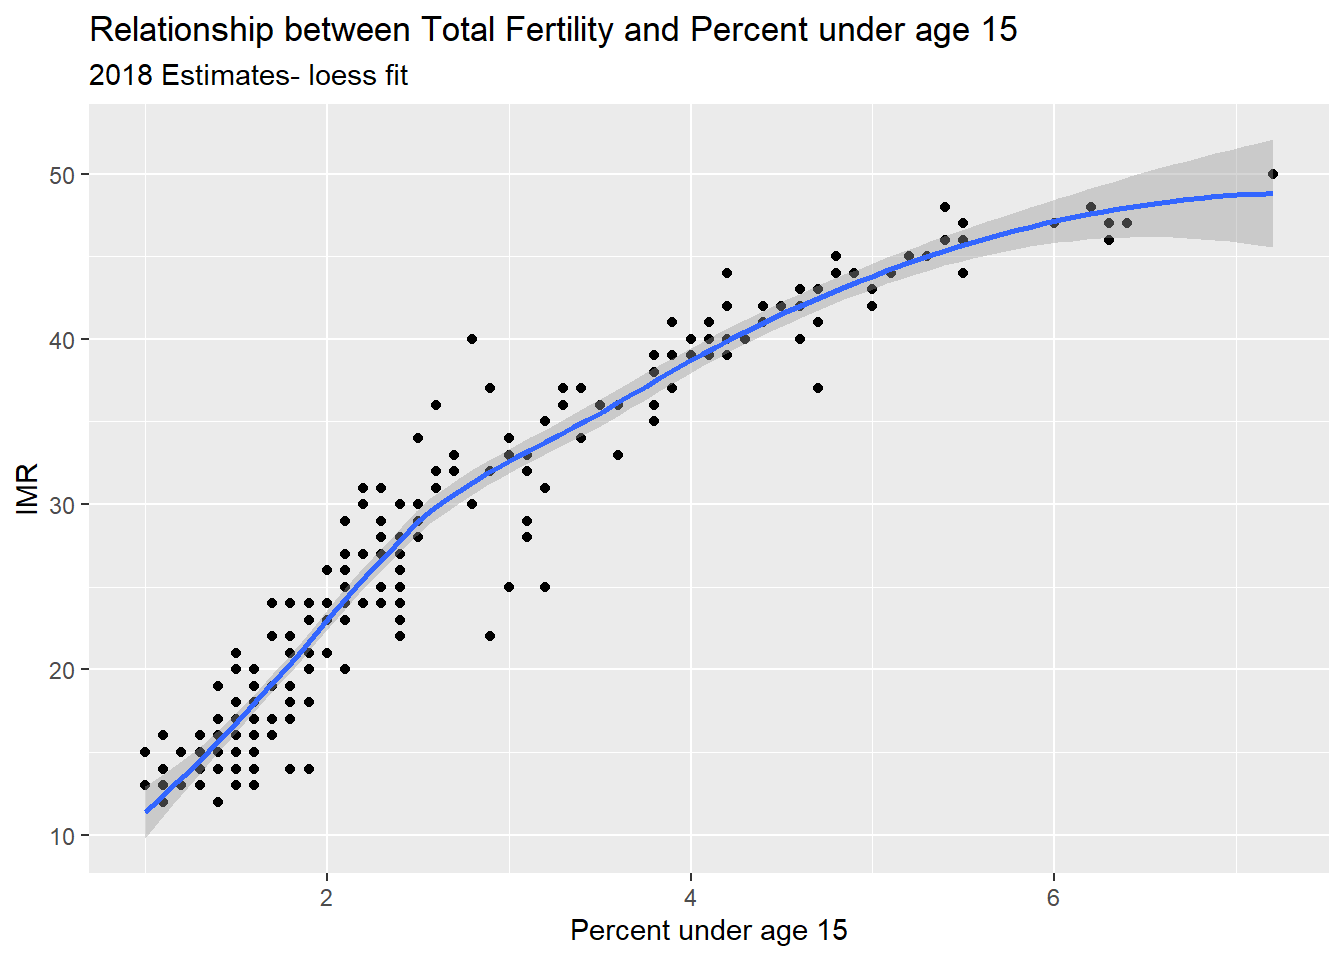
\includegraphics{macro_files/figure-pdf/unnamed-chunk-50-1.pdf}

}

\end{figure}

We see that the age distribution of Texas is slightly younger than
California, also the large peak at 25-34 year age group is because the
data adopt a 10 year age interval after age 25.

To do age standardization using the regression framework, we have to
control for the differences in the age structure of the two populations
(Texas and California) by regressing the mortality rate on the Age
structure, the difference between the states after doing this is the
difference in the age-standardized rate.

\begin{Shaded}
\begin{Highlighting}[]
\NormalTok{txca}\OtherTok{\textless{}{-}}\NormalTok{ txca}\SpecialCharTok{\%\textgreater{}\%}
  \FunctionTok{mutate}\NormalTok{(}\AttributeTok{Age\_Group =}\NormalTok{ forcats}\SpecialCharTok{::}\FunctionTok{fct\_relevel}\NormalTok{(txca}\SpecialCharTok{$}\NormalTok{Age\_Group,}\StringTok{"\textless{} 1 year"}\NormalTok{,}
                                    \StringTok{"1{-}4 years"}\NormalTok{,}
                                     \StringTok{"5{-}9 years"}\NormalTok{,}
                                    \StringTok{"10{-}14 years"}\NormalTok{,}
                                    \StringTok{"15{-}19 years"}\NormalTok{,}
                                    \StringTok{"20{-}24 years"}\NormalTok{,}
                                    \StringTok{"25{-}34 years"}\NormalTok{,}
                                    \StringTok{"35{-}44 years"}\NormalTok{,}
                                    \StringTok{"45{-}54 years"}\NormalTok{,}
                                    \StringTok{"55{-}64 years"}\NormalTok{,}
                                    \StringTok{"65{-}74 years"}\NormalTok{,}
                                    \StringTok{"75{-}84 years"}\NormalTok{, }\StringTok{"85+ years"}
\NormalTok{                                    ))}

\NormalTok{glmb\_s }\OtherTok{\textless{}{-}} \FunctionTok{glm}\NormalTok{(}\FunctionTok{cbind}\NormalTok{(Deaths, Population}\SpecialCharTok{{-}}\NormalTok{Deaths) }\SpecialCharTok{\textasciitilde{}} \FunctionTok{factor}\NormalTok{(Age\_Group)}\SpecialCharTok{+}\NormalTok{State,}
              \AttributeTok{data=}\NormalTok{txca,}
              \AttributeTok{family=}\NormalTok{binomial)}

\NormalTok{glmb\_s}\SpecialCharTok{\%\textgreater{}\%}
  \FunctionTok{tbl\_regression}\NormalTok{(}\AttributeTok{exp =} \ConstantTok{TRUE}\NormalTok{)}
\end{Highlighting}
\end{Shaded}

\begin{verbatim}
Table printed with `knitr::kable()`, not {gt}. Learn why at
https://www.danieldsjoberg.com/gtsummary/articles/rmarkdown.html
To suppress this message, include `message = FALSE` in code chunk header.
\end{verbatim}

\begin{tabular}{l|c|c|c}
\hline
**Characteristic** & **OR** & **95\% CI** & **p-value**\\
\hline
factor(Age\_Group) &  &  & \\
\hline
< 1 year & — & — & \\
\hline
1-4 years & 0.05 & 0.04, 0.05 & <0.001\\
\hline
5-9 years & 0.02 & 0.02, 0.03 & <0.001\\
\hline
10-14 years & 0.03 & 0.02, 0.03 & <0.001\\
\hline
15-19 years & 0.09 & 0.09, 0.10 & <0.001\\
\hline
20-24 years & 0.17 & 0.16, 0.18 & <0.001\\
\hline
25-34 years & 0.20 & 0.19, 0.21 & <0.001\\
\hline
35-44 years & 0.31 & 0.30, 0.32 & <0.001\\
\hline
45-54 years & 0.72 & 0.70, 0.75 & <0.001\\
\hline
55-64 years & 1.70 & 1.65, 1.75 & <0.001\\
\hline
65-74 years & 3.48 & 3.38, 3.59 & <0.001\\
\hline
75-84 years & 9.07 & 8.80, 9.35 & <0.001\\
\hline
85+ years & 30.4 & 29.5, 31.3 & <0.001\\
\hline
State &  &  & \\
\hline
California & — & — & \\
\hline
Texas & 1.20 & 1.19, 1.21 & <0.001\\
\hline
\end{tabular}

Which shows that Texas has a standardized mortality rate 20 percent
higher than California.

\hypertarget{poisson-distribution}{%
\section{Poisson distribution}\label{poisson-distribution}}

Another distribution commonly used in the analysis of place-based data
is the Poisson distribution. The Poisson is applicable to outcomes that
are positive integers, and is commonly used in epidemiology as a model
of relative risk of a disease or mortality. The Poisson has a single
parameter, the mean, \(\lambda\), and it is really the average count for
the outcome (\(y\)). We have several ways of modeling a count outcome
with the Poisson

\begin{itemize}
\tightlist
\item
  \emph{Pure count model} If each area or place has the same total area,
  risk set, or population size, then we can model the mean as-is. This
  would lead to a model that looks like:
\end{itemize}

\[log(\lambda)= \beta_0 + \beta_1 x_1\]

When we see the \(\beta_1\) parameter in this model in computer output,
it is on the log-scale, since that is the scale of the outcome for the
Poisson model. In order to interpret the \(\beta_1\), we have to
\textbf{\emph{exponentiate}} it. When we do this, the parameter is
interpreted as the \emph{percentage change in the mean of the outcome},
for a 1 unit change in \(x_1\). For instance if we estimate a model and
see in the output that \(\beta_1 = \text{.025}\), then
\(\exp(\beta_1) = \text{exp}(\text{.025}) = \text{1.025}\), or for a 1
unit increase in \(x_1\), the mean of \(y\) increases by 1.025. So if
the mean of \(y\) is 10, when \(x_1\) = 0, then the mean is
\(10*(1.025*1)\) or \(10.25\) when \(x_1\) = 1. This application of the
Poisson is rare in demographic research because places rarely have
either equal populations or areas, so the \emph{Rate Model} or the
\emph{Relative Risk Model} are much more commonly used.

\begin{itemize}
\tightlist
\item
  \emph{Rate model} The second type of modeling strategy used in the
  Poisson model is for a rate of occurrence. This model includes an
  \textbf{\emph{offset term}} in the model to incorporate unequal
  population sizes, this is the most common way the data are analyzed in
  demographic research. This offset term can be thought of as the
  denominator for the rate, and we can show how it is included in the
  model.
\end{itemize}

If \(n\) is the population size for each place, then, we want to do a
regression on the rate of occurrence of our outcome. The rate is
typically expressed as a proportion, or probability
\(rate = \frac{y}{n}\), as seen in the Binomial distribution earlier:

\[
log(y/n)= \beta_0 + \beta_1 x_1 \\
log(y) - log(n)= \beta_0 + \beta_1 x_1\\
log(y)= \beta_0 + \beta_1 x_1 + log(n)
\]

Similar to the example from before, when interpreting the effect of
\(\beta_1\) in this model, we also have to exponentiate it. In this
case, the interpretation would not be related to the overall count, but
to the rate of occurrence. So, if as before, the
\(\beta_1 = \text{.025}\), then
\(\exp(\beta_1) = \text{exp}(\text{.025}) = \text{1.025}\), or for a 1
unit increase in \(x_1\), the \textbf{\emph{rate}} of occurrence of
\(y\) increases by a factor of 1.025.

This model includes the natural log of the population size in the
\texttt{offset()} function on the right side of the model formula. R
will not estimate a regression coefficient for this term, and as in the
equation above, the term just represents a scale factor for the outcome.

\textbf{Note on offsets} It is important to ensure that all of the
populations in a particular analysis have non-zero counts, because if
the model sees \(log(0)\) in data, it will generate an error, because
this is not a number.

\begin{Shaded}
\begin{Highlighting}[]
\FunctionTok{log}\NormalTok{(}\DecValTok{0}\NormalTok{)}
\end{Highlighting}
\end{Shaded}

\begin{verbatim}
[1] -Inf
\end{verbatim}

The Poisson model with a population offset is specified as:

\begin{Shaded}
\begin{Highlighting}[]
\NormalTok{glmp\_s }\OtherTok{\textless{}{-}} \FunctionTok{glm}\NormalTok{(Deaths }\SpecialCharTok{\textasciitilde{}} \FunctionTok{offset}\NormalTok{(}\FunctionTok{log}\NormalTok{(Population)) }\SpecialCharTok{+} \FunctionTok{factor}\NormalTok{(Age\_Group) }\SpecialCharTok{+}\NormalTok{ State,}
              \AttributeTok{data=}\NormalTok{txca,}
              \AttributeTok{family=}\NormalTok{poisson)}

\NormalTok{glmp\_s}\SpecialCharTok{\%\textgreater{}\%}
  \FunctionTok{tbl\_regression}\NormalTok{(}\AttributeTok{exp =} \ConstantTok{TRUE}\NormalTok{)}
\end{Highlighting}
\end{Shaded}

\begin{verbatim}
Table printed with `knitr::kable()`, not {gt}. Learn why at
https://www.danieldsjoberg.com/gtsummary/articles/rmarkdown.html
To suppress this message, include `message = FALSE` in code chunk header.
\end{verbatim}

\begin{tabular}{l|c|c|c}
\hline
**Characteristic** & **IRR** & **95\% CI** & **p-value**\\
\hline
factor(Age\_Group) &  &  & \\
\hline
< 1 year & — & — & \\
\hline
1-4 years & 0.05 & 0.04, 0.05 & <0.001\\
\hline
5-9 years & 0.02 & 0.02, 0.03 & <0.001\\
\hline
10-14 years & 0.03 & 0.03, 0.03 & <0.001\\
\hline
15-19 years & 0.10 & 0.09, 0.10 & <0.001\\
\hline
20-24 years & 0.17 & 0.16, 0.18 & <0.001\\
\hline
25-34 years & 0.20 & 0.19, 0.21 & <0.001\\
\hline
35-44 years & 0.31 & 0.30, 0.32 & <0.001\\
\hline
45-54 years & 0.72 & 0.70, 0.75 & <0.001\\
\hline
55-64 years & 1.69 & 1.64, 1.74 & <0.001\\
\hline
65-74 years & 3.44 & 3.33, 3.54 & <0.001\\
\hline
75-84 years & 8.73 & 8.47, 9.00 & <0.001\\
\hline
85+ years & 26.6 & 25.8, 27.4 & <0.001\\
\hline
State &  &  & \\
\hline
California & — & — & \\
\hline
Texas & 1.19 & 1.18, 1.19 & <0.001\\
\hline
\end{tabular}

This result is very close to that from the Binomial model, where we see
after age standardization, Texas has a 19 percent higher mortality rate
overall than California.

\hypertarget{relative-risk-analysis}{%
\section{Relative risk analysis}\label{relative-risk-analysis}}

The third type of model for the Poisson distribution focuses on the idea
of the relative risk of an event, and uses the
\textbf{\emph{Standardized risk ratio}} as its currency.

\begin{itemize}
\tightlist
\item
  The \emph{Standardized risk ratio} incorporates differential exposure
  due to population size as an \textbf{\emph{expected count}} of the
  outcome in the offset term, and are typically seen in epidemiological
  studies. The expected count \(E\), incorporates the different
  population sizes of each area by estimating the number of events that
  \textbf{should occur}, if the area followed a given rate of
  occurrence. The expected count is calculated by multiplying the
  average rate of occurrence, \(r\), by the population size, \(n\):
  \(E_i = r * n_i\), where \(r = \frac{\sum y_i}{\sum n_i}\), is the
  overall rate in the population. This method is commonly referred to as
  \textbf{\emph{internal standardization}} because we are using the data
  at hand to estimate the overall rate of occurrence, versus using a
  rate from some other published source.
\end{itemize}

The model for the mean of the outcome would look like this:

\[log(y)= \beta_0 + \beta_1 x_1  + log(E)\].

And is specified very similarly to the rate model above. First, I show
how to calculate the expected number of deaths in the data. A naive
method of calculating the expected counts is to use the crude death rate
as \(r\), or we can use an age-specific death rate.

\begin{Shaded}
\begin{Highlighting}[]
\CommentTok{\#crude death rate}
\NormalTok{txca}\SpecialCharTok{$}\NormalTok{E}\OtherTok{\textless{}{-}}\NormalTok{ txca}\SpecialCharTok{$}\NormalTok{Population}\SpecialCharTok{*}\NormalTok{(}\FunctionTok{sum}\NormalTok{(txca}\SpecialCharTok{$}\NormalTok{Deaths}\SpecialCharTok{/}\FunctionTok{sum}\NormalTok{(txca}\SpecialCharTok{$}\NormalTok{Population)))}
\end{Highlighting}
\end{Shaded}

In this calculation, the \texttt{Population} variable is multiplied by
\(r\), which is the sum of all deaths, divided by all populations.

The age-specific expected count is a little more involved. We first have
to sum all deaths and populations by age, then calculate the age
specific rate, then join this back to the original data based on the
\texttt{Age\_Group} variable. Is this the only way to do this, no, but
it works in this example. Alternatively, we could get another age
schedule of mortality rates and merge it to these data and standardize
our data to that mortality schedule.

\begin{Shaded}
\begin{Highlighting}[]
\CommentTok{\#Age specific death rate}
\NormalTok{txca2}\OtherTok{\textless{}{-}}\NormalTok{ txca}\SpecialCharTok{\%\textgreater{}\%}
  \FunctionTok{group\_by}\NormalTok{(Age\_Group)}\SpecialCharTok{\%\textgreater{}\%}
  \FunctionTok{summarise}\NormalTok{(}\AttributeTok{ndeaths =} \FunctionTok{sum}\NormalTok{(Deaths), }\AttributeTok{npop=}\FunctionTok{sum}\NormalTok{(Population))}\SpecialCharTok{\%\textgreater{}\%}
  \FunctionTok{mutate}\NormalTok{(}\AttributeTok{r\_age =}\NormalTok{ ndeaths}\SpecialCharTok{/}\NormalTok{npop)}\SpecialCharTok{\%\textgreater{}\%}
  \FunctionTok{ungroup}\NormalTok{()}\SpecialCharTok{\%\textgreater{}\%}
  \FunctionTok{left\_join}\NormalTok{(., txca, }\AttributeTok{by =} \StringTok{"Age\_Group"}\NormalTok{)}\SpecialCharTok{\%\textgreater{}\%}
  \FunctionTok{arrange}\NormalTok{(State, Age\_Group)}\SpecialCharTok{\%\textgreater{}\%}
  \FunctionTok{mutate}\NormalTok{(}\AttributeTok{E\_age =}\NormalTok{ Population }\SpecialCharTok{*}\NormalTok{ r\_age)}

\NormalTok{txca2}\SpecialCharTok{\%\textgreater{}\%}
  \FunctionTok{select}\NormalTok{(State, Age\_Group, Deaths, Population, E, E\_age)}\SpecialCharTok{\%\textgreater{}\%}
  \FunctionTok{gt}\NormalTok{()}
\end{Highlighting}
\end{Shaded}

\begin{longtable*}{lcrrrr}
\toprule
State & Age\_Group & Deaths & Population & E & E\_age \\ 
\midrule
California & < 1 year & 2057 & 498832 & 3375.789 & 2395.1055 \\ 
California & 1-4 years & 397 & 1988540 & 13457.219 & 458.2383 \\ 
California & 5-9 years & 253 & 2539626 & 17186.631 & 293.4640 \\ 
California & 10-14 years & 277 & 2522475 & 17070.564 & 330.3049 \\ 
California & 15-19 years & 1076 & 2579986 & 17459.763 & 1176.4386 \\ 
California & 20-24 years & 2090 & 2812191 & 19031.184 & 2287.7627 \\ 
California & 25-34 years & 5201 & 5917785 & 40047.939 & 5682.6280 \\ 
California & 35-44 years & 7032 & 5159932 & 34919.255 & 7736.8039 \\ 
California & 45-54 years & 16370 & 5195297 & 35158.583 & 17888.9759 \\ 
California & 55-64 years & 34176 & 4688718 & 31730.368 & 37750.7084 \\ 
California & 65-74 years & 45834 & 3089002 & 20904.471 & 50503.1685 \\ 
California & 75-84 years & 59121 & 1535300 & 10389.969 & 63613.0044 \\ 
California & 85+ years & 88331 & 722333 & 4888.307 & 90772.2323 \\ 
Texas & < 1 year & 2287 & 405899 & 2746.875 & 1948.8945 \\ 
Texas & 1-4 years & 433 & 1613272 & 10917.635 & 371.7617 \\ 
Texas & 5-9 years & 276 & 2038319 & 13794.093 & 235.5360 \\ 
Texas & 10-14 years & 319 & 2029062 & 13731.447 & 265.6951 \\ 
Texas & 15-19 years & 999 & 1970588 & 13335.731 & 898.5614 \\ 
Texas & 20-24 years & 1829 & 2005169 & 13569.754 & 1631.2373 \\ 
Texas & 25-34 years & 4405 & 4085728 & 27649.701 & 3923.3720 \\ 
Texas & 35-44 years & 6292 & 3726287 & 25217.225 & 5587.1961 \\ 
Texas & 45-54 years & 13636 & 3519013 & 23814.522 & 12117.0241 \\ 
Texas & 55-64 years & 28663 & 3116019 & 21087.305 & 25088.2916 \\ 
Texas & 65-74 years & 37506 & 2008449 & 13591.951 & 32836.8315 \\ 
Texas & 75-84 years & 44144 & 957001 & 6476.396 & 39651.9956 \\ 
Texas & 85+ years & 51173 & 387790 & 2624.325 & 48731.7677 \\ 
\bottomrule
\end{longtable*}

In this table, you can see the age-specific expected counts of deaths
are much more in line with the age-specific mortality rate, and the
numbers of expected deaths are much more similar to the observed pattern
of deaths, when compared to the expected counts derived from the crude
death rate.

\begin{Shaded}
\begin{Highlighting}[]
\NormalTok{glmp\_E }\OtherTok{\textless{}{-}} \FunctionTok{glm}\NormalTok{(Deaths }\SpecialCharTok{\textasciitilde{}} \FunctionTok{offset}\NormalTok{(}\FunctionTok{log}\NormalTok{(E)) }\SpecialCharTok{+} \FunctionTok{factor}\NormalTok{(Age\_Group)}\SpecialCharTok{+}\NormalTok{State,}
              \AttributeTok{data=}\NormalTok{txca2,}
              \AttributeTok{family=}\NormalTok{poisson)}

\NormalTok{glmp\_Eage }\OtherTok{\textless{}{-}} \FunctionTok{glm}\NormalTok{(Deaths }\SpecialCharTok{\textasciitilde{}} \FunctionTok{offset}\NormalTok{(}\FunctionTok{log}\NormalTok{(E\_age)) }\SpecialCharTok{+} \FunctionTok{factor}\NormalTok{(Age\_Group)}\SpecialCharTok{+}\NormalTok{State,}
              \AttributeTok{data=}\NormalTok{txca2,}
              \AttributeTok{family=}\NormalTok{poisson)}

\NormalTok{m1 }\OtherTok{\textless{}{-}}\NormalTok{ glmp\_E}\SpecialCharTok{\%\textgreater{}\%}
  \FunctionTok{tbl\_regression}\NormalTok{(}\AttributeTok{exp =}\NormalTok{ T)}
\NormalTok{m2 }\OtherTok{\textless{}{-}}\NormalTok{ glmp\_Eage}\SpecialCharTok{\%\textgreater{}\%}
  \FunctionTok{tbl\_regression}\NormalTok{(}\AttributeTok{exp =}\NormalTok{ T)}

\NormalTok{m\_all }\OtherTok{\textless{}{-}} \FunctionTok{tbl\_merge}\NormalTok{(}\FunctionTok{list}\NormalTok{(m1, m2))}

\NormalTok{m\_all}
\end{Highlighting}
\end{Shaded}

\begin{verbatim}
Table printed with `knitr::kable()`, not {gt}. Learn why at
https://www.danieldsjoberg.com/gtsummary/articles/rmarkdown.html
To suppress this message, include `message = FALSE` in code chunk header.
\end{verbatim}

\begin{tabular}{l|c|c|c|c|c|c}
\hline
**Characteristic** & **IRR** & **95\% CI** & **p-value** & **IRR** & **95\% CI** & **p-value**\\
\hline
factor(Age\_Group) &  &  &  &  &  & \\
\hline
< 1 year & — & — &  & — & — & \\
\hline
1-4 years & 0.05 & 0.04, 0.05 & <0.001 & 1.00 & 0.93, 1.08 & >0.9\\
\hline
5-9 years & 0.02 & 0.02, 0.03 & <0.001 & 1.00 & 0.91, 1.09 & >0.9\\
\hline
10-14 years & 0.03 & 0.03, 0.03 & <0.001 & 1.00 & 0.92, 1.09 & >0.9\\
\hline
15-19 years & 0.10 & 0.09, 0.10 & <0.001 & 1.00 & 0.95, 1.06 & >0.9\\
\hline
20-24 years & 0.17 & 0.16, 0.18 & <0.001 & 1.01 & 0.96, 1.05 & 0.8\\
\hline
25-34 years & 0.20 & 0.19, 0.21 & <0.001 & 1.01 & 0.97, 1.04 & 0.7\\
\hline
35-44 years & 0.31 & 0.30, 0.32 & <0.001 & 1.01 & 0.97, 1.04 & 0.8\\
\hline
45-54 years & 0.72 & 0.70, 0.75 & <0.001 & 1.01 & 0.98, 1.04 & 0.6\\
\hline
55-64 years & 1.69 & 1.64, 1.74 & <0.001 & 1.01 & 0.98, 1.04 & 0.6\\
\hline
65-74 years & 3.44 & 3.33, 3.54 & <0.001 & 1.01 & 0.98, 1.04 & 0.5\\
\hline
75-84 years & 8.73 & 8.47, 9.00 & <0.001 & 1.01 & 0.98, 1.04 & 0.5\\
\hline
85+ years & 26.6 & 25.8, 27.4 & <0.001 & 1.02 & 0.99, 1.05 & 0.3\\
\hline
State &  &  &  &  &  & \\
\hline
California & — & — &  & — & — & \\
\hline
Texas & 1.19 & 1.18, 1.19 & <0.001 & 1.19 & 1.18, 1.19 & <0.001\\
\hline
\end{tabular}

This result is identical in terms of the difference between states, as
the rate model above, and the results are invariant to the choice of the
standard used, although when the age-specific expected count is used,
the overall mortality pattern becomes insignificant in the model. This
is an example of, despite different denominator/offset terms, we can
achieve the same comparison from either the rate model or the model for
relative risks.

\hypertarget{overdispersion}{%
\section{Overdispersion}\label{overdispersion}}

When using the Poisson GLM, you often run into \emph{overdispersion}.
What's overdispersion you might ask? For the Poisson distribution, the
mean and the variance are functions of one another (variance = mean for
Poisson). So when you have more variability than you expect in your
data, you have overdispersion. This basically says that your data do not
fit your model, and is a problem because overdispersion leads to
standard errors for our model parameters that are too small typically.
But, we can fit other models that do not make such assumptions, or allow
there to be more variability.

\hypertarget{checking-for-overdispersion}{%
\subsubsection{Checking for
overdispersion}\label{checking-for-overdispersion}}

An easy check on this is to compare the residual deviance to the
residual degrees of freedom. They ratio should be 1 if the model fits
the data.

\begin{Shaded}
\begin{Highlighting}[]
\NormalTok{scale}\OtherTok{\textless{}{-}}\FunctionTok{sqrt}\NormalTok{(glmp\_E}\SpecialCharTok{$}\NormalTok{deviance}\SpecialCharTok{/}\NormalTok{glmp\_E}\SpecialCharTok{$}\NormalTok{df.residual)}
\NormalTok{scale}
\end{Highlighting}
\end{Shaded}

Here, we see for the Poisson model, the scale factor is over 6, which
shows evidence of overdispersion in the data. The residual deviance can
also be used as a goodness of fit test for the model, because the
deviance has been shown to be distributed as a \(\chi^2\) distribution,
with degrees of freedom equal to the residual d.f. (n-p):

\begin{Shaded}
\begin{Highlighting}[]
\DecValTok{1}\SpecialCharTok{{-}}\FunctionTok{pchisq}\NormalTok{(glmp\_E}\SpecialCharTok{$}\NormalTok{deviance,}
         \AttributeTok{df =}\NormalTok{ glmp\_E}\SpecialCharTok{$}\NormalTok{df.residual)}
\end{Highlighting}
\end{Shaded}

So, this p value is 0, which means the model does not fit the data. If
the goodness of fit test had a p-value over 5 percent, we could conclude
that the model in fact did fit the data.

\hypertarget{modeling-overdispersion-via-a-quasi-distribution}{%
\section{Modeling Overdispersion via a Quasi
distribution}\label{modeling-overdispersion-via-a-quasi-distribution}}

For the Poisson and the Binomial, we can fit a ``quasi'' distribution
that adds an extra parameter to allow the mean-variance relationship to
not be constant. For Poisson we get:

\(Var(Y) = \lambda * \phi\), instead of \(Var(Y) = \lambda\)

This accessory parameter \(\phi\) allows us to include a rough proxy for
a dispersion parameter for the distribution. Naturally this is fixed at
1 for the normal Poisson model, and estimated in the quasi models, we
can look to see if is much bigger than 1. If overdispersion is present
and not accounted for you could identify a relationship as being
significant when it is not!

\begin{Shaded}
\begin{Highlighting}[]
\NormalTok{glmqp }\OtherTok{\textless{}{-}} \FunctionTok{glm}\NormalTok{(Deaths }\SpecialCharTok{\textasciitilde{}} \FunctionTok{offset}\NormalTok{(}\FunctionTok{log}\NormalTok{(E)) }\SpecialCharTok{+} \FunctionTok{factor}\NormalTok{(Age\_Group)}\SpecialCharTok{+}\NormalTok{State,}
              \AttributeTok{data=}\NormalTok{txca,}
              \AttributeTok{family=}\NormalTok{quasipoisson)}

\NormalTok{glmqp}\SpecialCharTok{\%\textgreater{}\%}
  \FunctionTok{tbl\_regression}\NormalTok{(}\AttributeTok{exp =} \ConstantTok{TRUE}\NormalTok{)}
\end{Highlighting}
\end{Shaded}

\begin{verbatim}
Table printed with `knitr::kable()`, not {gt}. Learn why at
https://www.danieldsjoberg.com/gtsummary/articles/rmarkdown.html
To suppress this message, include `message = FALSE` in code chunk header.
\end{verbatim}

\begin{tabular}{l|c|c|c}
\hline
**Characteristic** & **IRR** & **95\% CI** & **p-value**\\
\hline
factor(Age\_Group) &  &  & \\
\hline
< 1 year & — & — & \\
\hline
1-4 years & 0.05 & 0.03, 0.07 & <0.001\\
\hline
5-9 years & 0.02 & 0.01, 0.04 & <0.001\\
\hline
10-14 years & 0.03 & 0.02, 0.05 & <0.001\\
\hline
15-19 years & 0.10 & 0.07, 0.13 & <0.001\\
\hline
20-24 years & 0.17 & 0.13, 0.22 & <0.001\\
\hline
25-34 years & 0.20 & 0.16, 0.25 & <0.001\\
\hline
35-44 years & 0.31 & 0.25, 0.39 & <0.001\\
\hline
45-54 years & 0.72 & 0.59, 0.89 & 0.008\\
\hline
55-64 years & 1.69 & 1.40, 2.06 & <0.001\\
\hline
65-74 years & 3.44 & 2.85, 4.19 & <0.001\\
\hline
75-84 years & 8.73 & 7.25, 10.6 & <0.001\\
\hline
85+ years & 26.6 & 22.1, 32.4 & <0.001\\
\hline
State &  &  & \\
\hline
California & — & — & \\
\hline
Texas & 1.19 & 1.14, 1.23 & <0.001\\
\hline
\end{tabular}

While the overall pattern and substantive interpretation of the regular
Poisson and the quasiPoisson models are identical, the standard errors
of the parameters are not. We can see this by forming their ratios. The
standard errors of the model parameters can be extracted from the
\texttt{summary()\$coefficients} of a model, specifically the second
column of this table.

\begin{Shaded}
\begin{Highlighting}[]
\NormalTok{sum1}\OtherTok{\textless{}{-}} \FunctionTok{summary}\NormalTok{(glmp\_E)}\SpecialCharTok{$}\NormalTok{coef[, }\DecValTok{2}\NormalTok{]}
\NormalTok{sum2}\OtherTok{\textless{}{-}} \FunctionTok{summary}\NormalTok{(glmqp)}\SpecialCharTok{$}\NormalTok{coef[, }\DecValTok{2}\NormalTok{]}

\FunctionTok{data.frame}\NormalTok{(}\AttributeTok{Poisson =}\NormalTok{ sum1,}
           \AttributeTok{QPoisson=}\NormalTok{ sum2,}
           \AttributeTok{coef =} \FunctionTok{names}\NormalTok{(}\FunctionTok{coef}\NormalTok{(glmp\_E)))}\SpecialCharTok{\%\textgreater{}\%}
  \FunctionTok{ggplot}\NormalTok{(}\FunctionTok{aes}\NormalTok{(}\AttributeTok{y =}\NormalTok{ QPoisson}\SpecialCharTok{/}\NormalTok{Poisson, }\AttributeTok{x=}\NormalTok{ coef))}\SpecialCharTok{+}
  \FunctionTok{geom\_point}\NormalTok{()}\SpecialCharTok{+}
  \FunctionTok{ylab}\NormalTok{(}\StringTok{"Ratio of Standard Errors"}\NormalTok{ )}\SpecialCharTok{+}
  \FunctionTok{xlab}\NormalTok{ (}\StringTok{"Parameter"}\NormalTok{)}\SpecialCharTok{+}
  \FunctionTok{ggtitle}\NormalTok{(}\StringTok{"Ratio of Standard Errors in Poisson and QuasiPoisson Models"}\NormalTok{)}\SpecialCharTok{+}
  \FunctionTok{theme}\NormalTok{(}\AttributeTok{axis.text.x =} \FunctionTok{element\_text}\NormalTok{(}\AttributeTok{angle =} \DecValTok{45}\NormalTok{, }\AttributeTok{hjust =} \DecValTok{1}\NormalTok{))}
\end{Highlighting}
\end{Shaded}

\begin{figure}[H]

{\centering 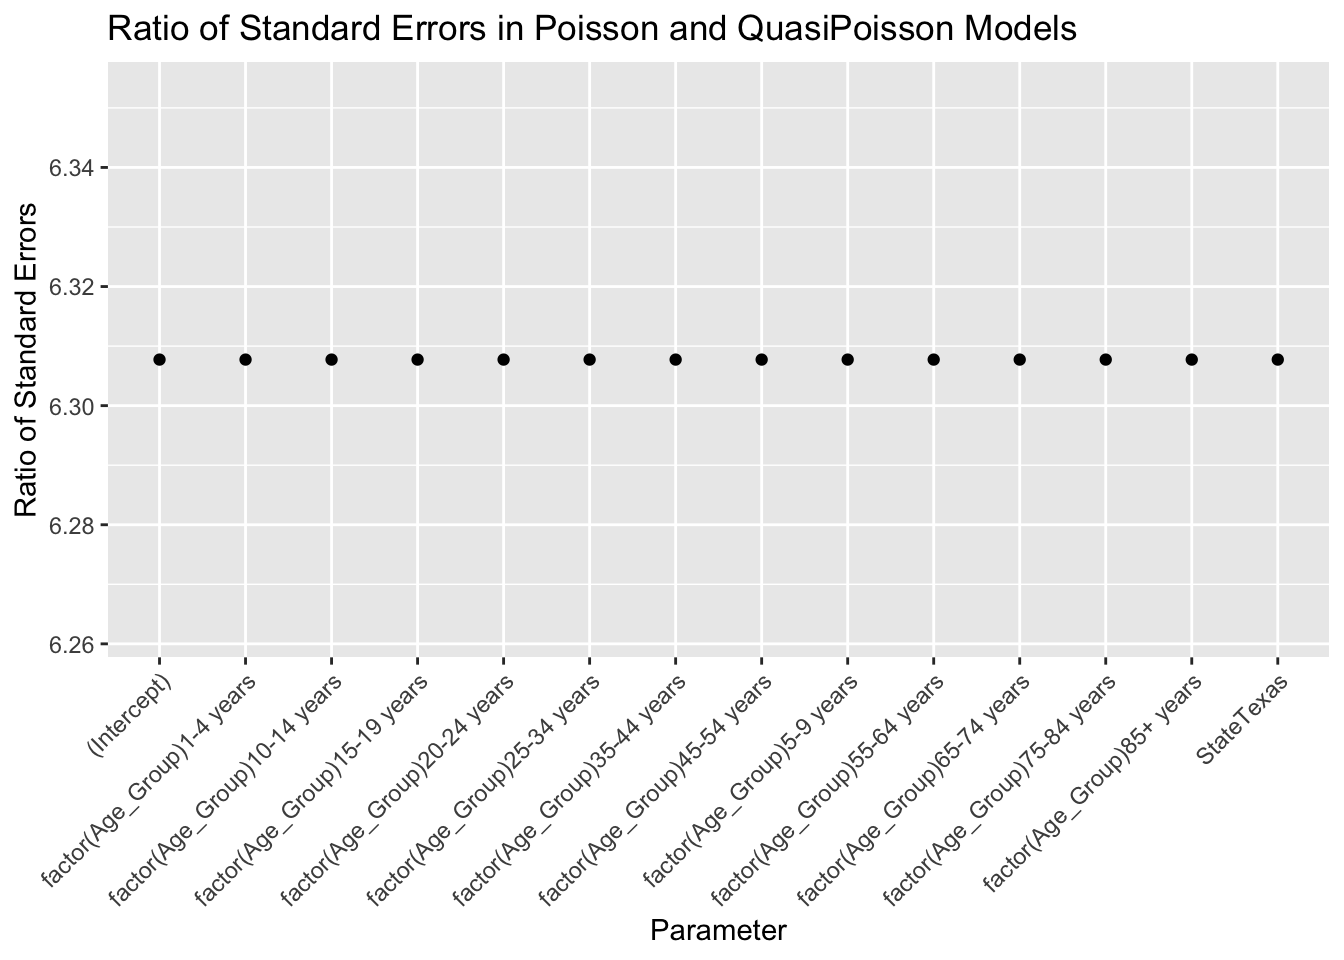
\includegraphics{macro_files/figure-pdf/unnamed-chunk-60-1.pdf}

}

\end{figure}

This \textbf{highly meaningful} plot shows the ratio of all the standard
errors is the same and is equal to the square root of the quasiPoisson
dispersion parameter \(\phi\), which can be seen in
\texttt{summary(glmqp)\$dispersion}, in this case it is 6.3079315, which
is extremely close to the \texttt{scale} we calculated earlier. The
quasiPoisson model has a disadvantage however, in that, per the
\texttt{?glm} documentation, is fit via quasi-likelihood methods and as
such cannot be compared using AIC to other models.

\hypertarget{modeling-dispersion-properly}{%
\subsection{Modeling dispersion
properly}\label{modeling-dispersion-properly}}

The \texttt{dispmod} package implements the method of Breslow (1984)
which adds an extra parameter to account for the overdispersion in the
Poisson, and is fit via regular maximum likelihood, so it is comparable
to other models. Effectively, this takes either a model fit via
\texttt{glm()} with either a Binomial or Poisson family, and performs a
re-weighted estimate of the model parameters.

\begin{Shaded}
\begin{Highlighting}[]
\FunctionTok{library}\NormalTok{(dispmod)}

\NormalTok{glmp\_d }\OtherTok{\textless{}{-}} \FunctionTok{glm.poisson.disp}\NormalTok{(glmp\_E,}
                           \AttributeTok{verbose =}\NormalTok{ F)}

\NormalTok{glmp\_d}\SpecialCharTok{\%\textgreater{}\%}
  \FunctionTok{tbl\_regression}\NormalTok{(}\AttributeTok{exp =}\NormalTok{ T)}
\end{Highlighting}
\end{Shaded}

\begin{verbatim}
Table printed with `knitr::kable()`, not {gt}. Learn why at
https://www.danieldsjoberg.com/gtsummary/articles/rmarkdown.html
To suppress this message, include `message = FALSE` in code chunk header.
\end{verbatim}

\begin{tabular}{l|c|c|c}
\hline
**Characteristic** & **IRR** & **95\% CI** & **p-value**\\
\hline
factor(Age\_Group) &  &  & \\
\hline
< 1 year & — & — & \\
\hline
1-4 years & 0.05 & 0.04, 0.05 & <0.001\\
\hline
5-9 years & 0.02 & 0.02, 0.03 & <0.001\\
\hline
10-14 years & 0.03 & 0.02, 0.03 & <0.001\\
\hline
15-19 years & 0.10 & 0.09, 0.10 & <0.001\\
\hline
20-24 years & 0.17 & 0.16, 0.19 & <0.001\\
\hline
25-34 years & 0.20 & 0.18, 0.22 & <0.001\\
\hline
35-44 years & 0.31 & 0.29, 0.34 & <0.001\\
\hline
45-54 years & 0.72 & 0.66, 0.79 & <0.001\\
\hline
55-64 years & 1.70 & 1.56, 1.85 & <0.001\\
\hline
65-74 years & 3.45 & 3.16, 3.76 & <0.001\\
\hline
75-84 years & 8.73 & 8.01, 9.52 & <0.001\\
\hline
85+ years & 26.4 & 24.2, 28.8 & <0.001\\
\hline
State &  &  & \\
\hline
California & — & — & \\
\hline
Texas & 1.24 & 1.20, 1.29 & <0.001\\
\hline
\end{tabular}

In this example the difference between California and Texas is now
larger at a 24\% higher mortality rate in Texas. How does this model
compare to the regular Poisson model?

\begin{Shaded}
\begin{Highlighting}[]
\FunctionTok{AIC}\NormalTok{(glmp\_E, glmp\_d)}
\end{Highlighting}
\end{Shaded}

\begin{verbatim}
       df      AIC
glmp_E 14 773.7668
glmp_d 14  90.3267
\end{verbatim}

The dispersed model shows a much lower AIC suggesting that the
dispersion accounted for in the the Breslow model is likely important.
We can see how the dispersed Poisson model's standard errors compare to
those of the regular Poisson using the same plot we saw earlier:

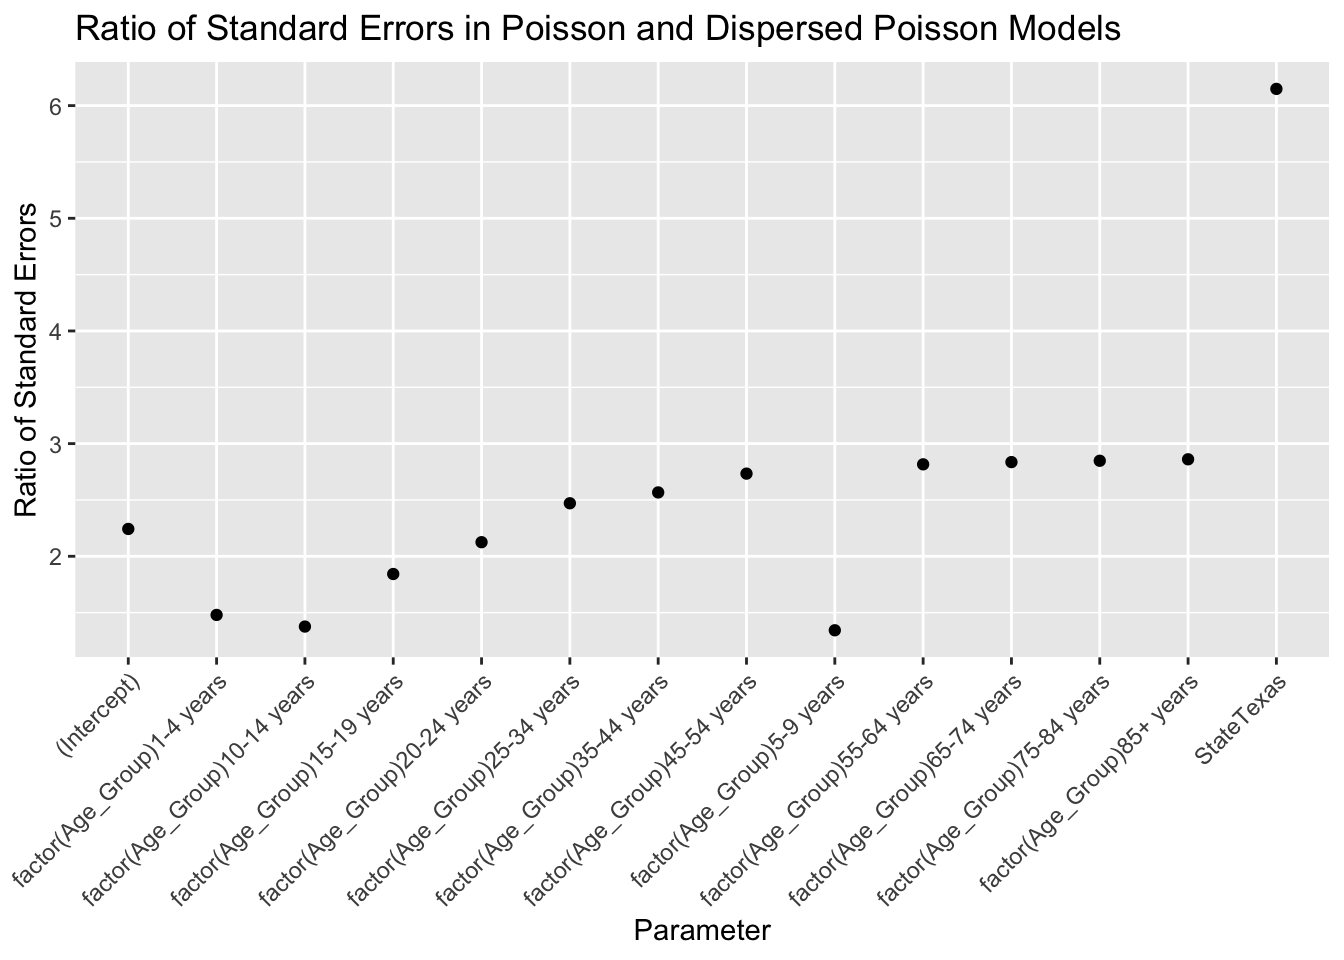
\includegraphics{macro_files/figure-pdf/unnamed-chunk-63-1.pdf}

In this case, the standard errors are not just a monotone transformation
of the Poisson model errors, they each have their own scaling, which
shows the dispersed Poisson model is doing something different compared
to the quasiPoisson model by not using a single scaling factor for all
the standard errors.

\hypertarget{other-count-models}{%
\section{Other count models}\label{other-count-models}}

The Poisson and Binomial models are probably the most commonly used
models for rates and proportions, but other models exist that offer more
flexibility. Specifically the Beta distribution and the Negative
Binomial distribution.

\hypertarget{beta-distribution-model}{%
\subsection{Beta distribution model}\label{beta-distribution-model}}

The Beta distribution is a commonly used model for the prior
distribution for the mean of the Binomial, as it has values between 0
and 1, but it is not used as often as an outcome distribution. It is
indeed quite flexible as an outcome distribution for proportions because
of its range of support, but also because it has an additional
dispersion parameter, unlike the Binomial, so the pitfalls of
overdispersion often present in the Binomial can be avoided. The
\texttt{betareg} package (Grün, Kosmidis, and Zeileis 2012) implements
the Beta regression model. The distribution has density:

\[
f(y:p,q) = \frac{\Gamma(p +
q)}{\Gamma(p)\Gamma(q)}x^{p - 1}(1 - x)^{q - 1}
\] Where \(\Gamma\) is the Gamma function. The distribution, as
parameterized in \texttt{betareg} has mean and variance:

\[
\mu = p/(p+q) \\
Var = \mu (1-\mu)/ (1+\phi)
\]

Where \(phi\) is a precision parameter. The model is linked to the
linear predictor using one of the same link functions as the Binomial
model: Logit, Probit or Complementary Log-Log.

\[g(\mu_i) = X'\beta = \eta_i\] The Logit link is parameterized as:

\[logit(g(\mu)) = log(\mu / (1-\mu))\] As described in their article on
the \texttt{betareg} package (Cribari-Neto and Zeileis 2010), the model
can also include a separate model for dispersion, so you can model the
variance in the data as well as the mean.

The \texttt{betareg::betareg()} function implements model, and here is
an application of the model to the low birth weight data used earlier:

\begin{Shaded}
\begin{Highlighting}[]
\FunctionTok{library}\NormalTok{(betareg)}
\NormalTok{glm\_beta}\OtherTok{\textless{}{-}}\FunctionTok{betareg}\NormalTok{(}\FunctionTok{I}\NormalTok{(lbrate1618}\SpecialCharTok{/}\DecValTok{1000}\NormalTok{) }\SpecialCharTok{\textasciitilde{}}\NormalTok{  fampov14 }\SpecialCharTok{+}\NormalTok{ rucc }\SpecialCharTok{+}\NormalTok{ hpsa16, }
                  \AttributeTok{data=}\NormalTok{ahrf\_m)}

\FunctionTok{summary}\NormalTok{(glm\_beta)}
\end{Highlighting}
\end{Shaded}

\begin{verbatim}

Call:
betareg(formula = I(lbrate1618/1000) ~ fampov14 + rucc + hpsa16, data = ahrf_m)

Standardized weighted residuals 2:
    Min      1Q  Median      3Q     Max 
-7.0393 -0.6234 -0.0110  0.6338  3.7500 

Coefficients (mean model with logit link):
                                Estimate Std. Error  z value Pr(>|z|)    
(Intercept)                   -2.6387868  0.0150612 -175.204  < 2e-16 ***
fampov14                       0.0252868  0.0007936   31.862  < 2e-16 ***
rucc02                        -0.0188140  0.0150716   -1.248 0.211917    
rucc03                        -0.0400036  0.0157581   -2.539 0.011129 *  
rucc04                        -0.0798596  0.0177856   -4.490 7.12e-06 ***
rucc05                        -0.0734111  0.0242750   -3.024 0.002493 ** 
rucc06                        -0.0494087  0.0142816   -3.460 0.000541 ***
rucc07                        -0.0498176  0.0159746   -3.119 0.001817 ** 
rucc08                         0.0038585  0.0252486    0.153 0.878541    
rucc09                        -0.0636793  0.0274465   -2.320 0.020334 *  
hpsa16partial county shortage -0.0019801  0.0128139   -0.155 0.877196    
hpsa16whole county shortage    0.0278359  0.0156183    1.782 0.074706 .  

Phi coefficients (precision model with identity link):
      Estimate Std. Error z value Pr(>|z|)    
(phi)  304.733      8.948   34.06   <2e-16 ***
---
Signif. codes:  0 '***' 0.001 '**' 0.01 '*' 0.05 '.' 0.1 ' ' 1 

Type of estimator: ML (maximum likelihood)
Log-likelihood:  6347 on 13 Df
Pseudo R-squared: 0.355
Number of iterations: 23 (BFGS) + 3 (Fisher scoring) 
\end{verbatim}

And the model with a separate model for the dispersion can be estimated
by including a second formula separated by a \texttt{\textbar{}} as:

\begin{Shaded}
\begin{Highlighting}[]
\FunctionTok{library}\NormalTok{(betareg)}
\NormalTok{glm\_beta\_o}\OtherTok{\textless{}{-}}\FunctionTok{betareg}\NormalTok{(}\FunctionTok{I}\NormalTok{(lbrate1618}\SpecialCharTok{/}\DecValTok{1000}\NormalTok{) }\SpecialCharTok{\textasciitilde{}}\NormalTok{  fampov14 }\SpecialCharTok{+}\NormalTok{ rucc }\SpecialCharTok{+}\NormalTok{ hpsa16 }\SpecialCharTok{|} \FunctionTok{scale}\NormalTok{(popn), }
                  \AttributeTok{data=}\NormalTok{ahrf\_m)}

\FunctionTok{summary}\NormalTok{(glm\_beta\_o)}
\end{Highlighting}
\end{Shaded}

\begin{verbatim}

Call:
betareg(formula = I(lbrate1618/1000) ~ fampov14 + rucc + hpsa16 | scale(popn), 
    data = ahrf_m)

Standardized weighted residuals 2:
    Min      1Q  Median      3Q     Max 
-6.9251 -0.6169 -0.0023  0.6500  3.7111 

Coefficients (mean model with logit link):
                                Estimate Std. Error  z value Pr(>|z|)    
(Intercept)                   -2.6421609  0.0149203 -177.085  < 2e-16 ***
fampov14                       0.0251141  0.0007938   31.639  < 2e-16 ***
rucc02                        -0.0124912  0.0146382   -0.853  0.39348    
rucc03                        -0.0327516  0.0154238   -2.123  0.03372 *  
rucc04                        -0.0721414  0.0175194   -4.118 3.83e-05 ***
rucc05                        -0.0655256  0.0241470   -2.714  0.00666 ** 
rucc06                        -0.0415704  0.0139537   -2.979  0.00289 ** 
rucc07                        -0.0417441  0.0156940   -2.660  0.00782 ** 
rucc08                         0.0118585  0.0252317    0.470  0.63837    
rucc09                        -0.0550535  0.0274518   -2.005  0.04491 *  
hpsa16partial county shortage -0.0048007  0.0127864   -0.375  0.70733    
hpsa16whole county shortage    0.0270952  0.0156837    1.728  0.08406 .  

Phi coefficients (precision model with log link):
            Estimate Std. Error z value Pr(>|z|)    
(Intercept)  5.72714    0.02936 195.063  < 2e-16 ***
scale(popn)  0.08419    0.02929   2.874  0.00405 ** 
---
Signif. codes:  0 '***' 0.001 '**' 0.01 '*' 0.05 '.' 0.1 ' ' 1 

Type of estimator: ML (maximum likelihood)
Log-likelihood:  6355 on 14 Df
Pseudo R-squared: 0.3548
Number of iterations: 21 (BFGS) + 5 (Fisher scoring) 
\end{verbatim}

The AIC can be used to determine if the dispersion model is preferred to
the regular beta regression.

\begin{Shaded}
\begin{Highlighting}[]
\FunctionTok{AIC}\NormalTok{(glm\_beta, glm\_beta\_o)}
\end{Highlighting}
\end{Shaded}

\begin{verbatim}
           df       AIC
glm_beta   13 -12668.24
glm_beta_o 14 -12682.02
\end{verbatim}

In this case, the dispersion model is preferred since the AIC is 13.78
points lower for the dispersion model.

\hypertarget{negative-binomial-model}{%
\subsection{Negative binomial model}\label{negative-binomial-model}}

When overdispersion is present, many researchers will automatically turn
to the Negative Binomial as an alternative. The Negative Binomial sounds
like it is some alternative to the Binomial distribution, but it is more
like the Poisson. It effectively adds a second parameter to a model for
integer counts. The model has been parameterized in several ways. The
most common are the NB1 and NB2 models. The difference is how the model
allows the variance to increase with the mean. The NB1 model allows for
variance to increase linearly with the mean:

\[
Y \sim NB (\lambda, \lambda+ \theta \lambda) \\
E(Y) = \lambda \\
\text{   } var(Y) = \lambda+\theta\lambda \\
\lambda = log(\eta) \\ 
\eta = \beta_0 + \beta_1 x_1+ log(n)
\] The NB2 model, which is the most commonly implemented in software,
allows the variance to increase as a square with the mean.

\[
Y \sim NB (\lambda, \lambda+ \theta \lambda^2) \\
E(Y) = \lambda \\
\text{   } var(Y) = \lambda+ \theta \lambda^2 \\
\lambda = log(\eta) \\ 
\eta = \beta_0 + \beta_1 x_1+ log(n)
\]

The base R \texttt{glm()} does not offer the NB1 model by default, but
the standard \texttt{MASS} package (Venables and Ripley 2002) has the
\texttt{glm.nb()} function. An alternative is the highly flexible
\texttt{gamlss} package(Rigby and Stasinopoulos 2005), which includes
the NB2 model, as well as a host of other distributions, plus the
ability to model mean and variance, similar to how \texttt{betareg()}
was achieving for the Beta distribution.

\begin{Shaded}
\begin{Highlighting}[]
\FunctionTok{library}\NormalTok{(MASS)}
\end{Highlighting}
\end{Shaded}

\begin{verbatim}

Attaching package: 'MASS'
\end{verbatim}

\begin{verbatim}
The following object is masked from 'package:gtsummary':

    select
\end{verbatim}

\begin{verbatim}
The following object is masked from 'package:dplyr':

    select
\end{verbatim}

\begin{Shaded}
\begin{Highlighting}[]
\NormalTok{glmnb}\OtherTok{\textless{}{-}} \FunctionTok{glm.nb}\NormalTok{(lowbw1618 }\SpecialCharTok{\textasciitilde{}} \FunctionTok{offset}\NormalTok{(}\FunctionTok{log}\NormalTok{(births1618)) }\SpecialCharTok{+}\NormalTok{ fampov14 }\SpecialCharTok{+}\NormalTok{ rucc }\SpecialCharTok{+}\NormalTok{ hpsa16 ,}
               \AttributeTok{data=}\NormalTok{ahrf\_m)}


\NormalTok{glmnb}\SpecialCharTok{\%\textgreater{}\%}
  \FunctionTok{tbl\_regression}\NormalTok{()}
\end{Highlighting}
\end{Shaded}

\begin{verbatim}
Table printed with `knitr::kable()`, not {gt}. Learn why at
https://www.danieldsjoberg.com/gtsummary/articles/rmarkdown.html
To suppress this message, include `message = FALSE` in code chunk header.
\end{verbatim}

\begin{tabular}{l|c|c|c}
\hline
**Characteristic** & **log(IRR)** & **95\% CI** & **p-value**\\
\hline
\% Families Below Poverty Level 2014-18 & 0.03 & 0.02, 0.03 & <0.001\\
\hline
rucc &  &  & \\
\hline
01 & — & — & \\
\hline
02 & -0.02 & -0.04, 0.01 & 0.2\\
\hline
03 & -0.04 & -0.07, -0.02 & <0.001\\
\hline
04 & -0.08 & -0.11, -0.05 & <0.001\\
\hline
05 & -0.07 & -0.12, -0.03 & <0.001\\
\hline
06 & -0.06 & -0.08, -0.03 & <0.001\\
\hline
07 & -0.07 & -0.10, -0.04 & <0.001\\
\hline
08 & -0.01 & -0.07, 0.06 & 0.9\\
\hline
09 & -0.09 & -0.16, -0.01 & 0.021\\
\hline
hpsa16 &  &  & \\
\hline
no shortage & — & — & \\
\hline
partial county shortage & -0.01 & -0.03, 0.01 & 0.4\\
\hline
whole county shortage & 0.00 & -0.03, 0.03 & >0.9\\
\hline
\end{tabular}

The NB2 version of the model can be estimated using \texttt{gamlss()}
with \texttt{family=NBII}:

\begin{Shaded}
\begin{Highlighting}[]
\FunctionTok{library}\NormalTok{(gamlss)}
\end{Highlighting}
\end{Shaded}

\begin{verbatim}
Loading required package: gamlss.data
\end{verbatim}

\begin{verbatim}

Attaching package: 'gamlss.data'
\end{verbatim}

\begin{verbatim}
The following object is masked from 'package:datasets':

    sleep
\end{verbatim}

\begin{verbatim}
Loading required package: gamlss.dist
\end{verbatim}

\begin{verbatim}
Loading required package: parallel
\end{verbatim}

\begin{verbatim}
Registered S3 method overwritten by 'gamlss':
  method   from
  print.ri bit 
\end{verbatim}

\begin{verbatim}
 **********   GAMLSS Version 5.4-12  ********** 
\end{verbatim}

\begin{verbatim}
For more on GAMLSS look at https://www.gamlss.com/
\end{verbatim}

\begin{verbatim}
Type gamlssNews() to see new features/changes/bug fixes.
\end{verbatim}

\begin{Shaded}
\begin{Highlighting}[]
\NormalTok{glmnb2}\OtherTok{\textless{}{-}}\FunctionTok{gamlss}\NormalTok{(lowbw1618 }\SpecialCharTok{\textasciitilde{}} \FunctionTok{offset}\NormalTok{(}\FunctionTok{log}\NormalTok{(births1618)) }\SpecialCharTok{+}\NormalTok{ fampov14 }\SpecialCharTok{+}\NormalTok{ rucc }\SpecialCharTok{+}\NormalTok{ hpsa16,}
               \AttributeTok{family =}\NormalTok{ NBII,}
               \AttributeTok{data=}\NormalTok{ahrf\_m)}
\end{Highlighting}
\end{Shaded}

\begin{verbatim}
GAMLSS-RS iteration 1: Global Deviance = 27778.63 
GAMLSS-RS iteration 2: Global Deviance = 26730.85 
GAMLSS-RS iteration 3: Global Deviance = 25316.94 
GAMLSS-RS iteration 4: Global Deviance = 23326.65 
GAMLSS-RS iteration 5: Global Deviance = 20580.7 
GAMLSS-RS iteration 6: Global Deviance = 18480.22 
GAMLSS-RS iteration 7: Global Deviance = 18277.94 
GAMLSS-RS iteration 8: Global Deviance = 18277.03 
GAMLSS-RS iteration 9: Global Deviance = 18277.03 
GAMLSS-RS iteration 10: Global Deviance = 18277.03 
\end{verbatim}

\begin{Shaded}
\begin{Highlighting}[]
\FunctionTok{summary}\NormalTok{(glmnb2)}
\end{Highlighting}
\end{Shaded}

\begin{verbatim}
******************************************************************
Family:  c("NBII", "Negative Binomial type II") 

Call:  gamlss(formula = lowbw1618 ~ offset(log(births1618)) +  
    fampov14 + rucc + hpsa16, family = NBII, data = ahrf_m) 

Fitting method: RS() 

------------------------------------------------------------------
Mu link function:  log
Mu Coefficients:
                                Estimate Std. Error  t value Pr(>|t|)    
(Intercept)                   -2.6762604  0.0122536 -218.407   <2e-16 ***
fampov14                       0.0189986  0.0006901   27.532   <2e-16 ***
rucc02                        -0.0124200  0.0080482   -1.543   0.1229    
rucc03                        -0.0166503  0.0113856   -1.462   0.1438    
rucc04                        -0.0401176  0.0163552   -2.453   0.0142 *  
rucc05                        -0.0291354  0.0254089   -1.147   0.2516    
rucc06                         0.0058763  0.0161169    0.365   0.7154    
rucc07                         0.0068020  0.0211064    0.322   0.7473    
rucc08                         0.0941871  0.0493463    1.909   0.0564 .  
rucc09                         0.0208654  0.0546114    0.382   0.7024    
hpsa16partial county shortage -0.0203470  0.0117608   -1.730   0.0838 .  
hpsa16whole county shortage    0.0082867  0.0195254    0.424   0.6713    
---
Signif. codes:  0 '***' 0.001 '**' 0.01 '*' 0.05 '.' 0.1 ' ' 1

------------------------------------------------------------------
Sigma link function:  log
Sigma Coefficients:
            Estimate Std. Error t value Pr(>|t|)    
(Intercept)  0.72887    0.04354   16.74   <2e-16 ***
---
Signif. codes:  0 '***' 0.001 '**' 0.01 '*' 0.05 '.' 0.1 ' ' 1

------------------------------------------------------------------
No. of observations in the fit:  2324 
Degrees of Freedom for the fit:  13
      Residual Deg. of Freedom:  2311 
                      at cycle:  10 
 
Global Deviance:     18277.03 
            AIC:     18303.03 
            SBC:     18377.79 
******************************************************************
\end{verbatim}

Again, between these two different specifications, we see very similar
results. We can compare each of the models, starting with the Gaussian
model and proceeding through the NB2 model above (although the Beta
regression appears to be on a different scale since the outcome is
specified as probability, versus a count, so it is not comparable to the
rest) using the \texttt{AIC()} function:

\begin{Shaded}
\begin{Highlighting}[]
\FunctionTok{AIC}\NormalTok{(glm1, glmb, glmp\_b, glmnb, glmnb2)}
\end{Highlighting}
\end{Shaded}

\begin{verbatim}
       df      AIC
glm1   13 19599.34
glmb   12 20980.41
glmp_b 12 20517.93
glmnb  13 16866.26
glmnb2 13 18303.03
\end{verbatim}

We see that among these five model specifications, the Binomial fits the
worst and the NB1 model, estimated by \texttt{glm.nb()} fits the best,
with the lowest AIC among these five models.

\bookmarksetup{startatroot}

\hypertarget{event-history-models-for-microdemography}{%
\chapter{Event History Models for
Microdemography}\label{event-history-models-for-microdemography}}

\newpage

\bookmarksetup{startatroot}

\hypertarget{micro-demography}{%
\chapter{Micro-demography}\label{micro-demography}}

Demographic studies began to focus on individual level outcomes once the
availability of individual level census and social/health survey data
became more prevalent in the 1960's and 1970's. Corresponding with this
availability of individual level data, demography began to be influenced
by sociological thought, which brought a proper theoretical perspective
to demographic studies, which, before this period were dominated by
methodological issues and descriptions of macro scale demographic
processes we saw in the previous chapter.

This chapter focuses on how we model individual level observational
data, with a focus on data from demographic surveys. In doing this, I
focus on two primary goals, first to illustrate how to conduct commonly
used regression analysis of demographic outcomes as measured in surveys,
drawing heavily on data from the ******. Secondly, I describe the
event-history framework that is used in much of social science when we
analyze changes in outcomes between time points, or in describing the
time to some demographic event, such as having a child or dying.

\hypertarget{individual-level-focus}{%
\subsection{Individual-level focus}\label{individual-level-focus}}

In contrast to the macro-demographic perspective described in the
previous chapter, the micro-demographic perspective is focused on the
\textbf{individual} rather than the aggregate. Barbara Entwisle (2007)
explains, micro-demography focuses on how individuals are modeled within
demographic studies, which focus on individual level behaviors and
outcomes as a prime importance. Most of the time in an individual, or
micro-demographic focus, our hypotheses are related to how the
individual outcome or behavior is influenced by characteristics of the
individual, usually without concern or interest in the physical or
social context in which the individual lives their life. For instance,
in a micro-demographic study of mortality, the researcher may make ask:
\emph{Do individuals with a low level of education face higher risk of
death, compared to people with a college education} This in and of
itself says nothing about the spatial context in which the person lives,
it is only concerned with characteristics of the person.

\hypertarget{individual-level-propositions}{%
\subsection{Individual level
propositions}\label{individual-level-propositions}}

If we are concerned with how individual-level factors affect each
person's outcome, then we are stating an individual level, or micro,
proposition. In this type of analysis, we have \emph{y} and \emph{x},
both measured on our individual level units. We may also have a variable
\emph{Z} measured on a second-level unit, but we'll wait and discuss
these in the next chapter. An example of this micro-level, or individual
level, proposition would be that we think a persons health is affected
by their level of education.

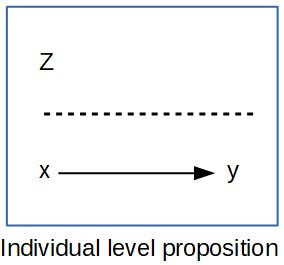
\includegraphics{./images/indi.png} \#\# Types of individual level
outcomes In the analysis of micro-demographic outcomes, we encounter a
wide variety of outcomes. Some are relatively simple recoding of
existing survey data, other times the outcomes depend on repeated
measures of some behavior in a longitudinal framework. At the heart of
different outcomes are different assumed statistical distributions used
to model them, and the choices that we face related to which outcome
best suits a particular outcome. Based on the Generalized Linear Model
framework introduced in the previous chapter, in this chapter my goal is
to illustrate how to use this framework for analyzing a variety of
different types of outcomes. Also, I show how to use appropriate
corrections for using complex survey data in the context of the various
outcome types, relying heavily on the \texttt{survey} and
\texttt{svyVGAM} packages (Lumley 2004, 2021).

\hypertarget{continuous-outcomes}{%
\subsection{Continuous outcomes}\label{continuous-outcomes}}

The workhorse for continuous outcomes in statistics is the Gaussian, or
Normal distribution linear model, which was reviewed in the previous
chapter. The Normal distribution is incredibly flexible in its form, and
once certain restrictions are removed via techniques such as generalized
least squares, the model becomes even more flexible. I do not intend to
go over the details of the model estimation in this chapter, as this was
covered previously. Instead, I will use a common demographic survey data
source, the Demographic and Health Survey model data to illustrate how
to include survey design information and estimate the models. In
addition to the Normal distribution, other continuous distributions
including the Student-t and Gamma distributions are also relevant for
modeling heteroskedastic and skewed continuous outcomes, as described in
the previous chapters.

\hypertarget{data-for-examples}{%
\subsubsection{Data for examples}\label{data-for-examples}}

\hypertarget{discrete}{%
\subsubsection{Discrete}\label{discrete}}

\hypertarget{binary-logistic-regression-model}{%
\subsubsection{Binary Logistic regression
model}\label{binary-logistic-regression-model}}

\hypertarget{marginal-effects}{%
\subsubsection{Marginal effects}\label{marginal-effects}}

\hypertarget{ordinal-logistic-regression-model}{%
\subsubsection{Ordinal logistic regression
model}\label{ordinal-logistic-regression-model}}

\hypertarget{multinomial-logistic-regression-model}{%
\subsubsection{Multinomial logistic regression
model}\label{multinomial-logistic-regression-model}}

\hypertarget{changes-in-an-outcome-over-time}{%
\subsubsection{Changes in an outcome over
time}\label{changes-in-an-outcome-over-time}}

\hypertarget{creating-an-event-history-dataset}{%
\subsubsection{Creating an event history
dataset}\label{creating-an-event-history-dataset}}

\hypertarget{creating-a-longitudinal-dataset}{%
\subsection{Creating a longitudinal
dataset}\label{creating-a-longitudinal-dataset}}

\hypertarget{event-history-framework}{%
\section{Event history framework}\label{event-history-framework}}

\hypertarget{when-to-conduct-an-event-history-analysis}{%
\subsection{When to conduct an event history
analysis?}\label{when-to-conduct-an-event-history-analysis}}

\begin{itemize}
\tightlist
\item
  When you questions include

  \begin{itemize}
  \tightlist
  \item
    When or Whether
  \item
    When \textgreater{} how long until an event occurs
  \item
    Whether \textgreater{} does an event occur or not
  \end{itemize}
\item
  If your question does not include either of these ideas (or cannot be
  made to) then you do not need to do event history analysis
\end{itemize}

\hypertarget{basic-propositions}{%
\subsection{Basic Propositions}\label{basic-propositions}}

\begin{itemize}
\tightlist
\item
  Since most of the methods we will discuss originate from studies of
  mortality, they have morbid names

  \begin{itemize}
  \tightlist
  \item
    Survival -- This is related to how long a case lasts until it
    experiences the event of interest
  \item
    How long does it take?
  \item
    Risk -- How likely is it that the case will experience the event
  \item
    Will it happen or not?
  \end{itemize}
\end{itemize}

\hypertarget{focus-on-comparison}{%
\subsection{Focus on comparison}\label{focus-on-comparison}}

\begin{itemize}
\tightlist
\item
  Most of the methods we consider are comparative by their nature
\item
  How long does a case with trait x survive, compared to a case with
  trait y?
\item
  How likely is it for a person who is married to die of homicide
  relative to someone who is single?
\item
  Generally we are examining relative risk and relative survival
\end{itemize}

\hypertarget{some-terminology}{%
\subsection{Some terminology}\label{some-terminology}}

\begin{itemize}
\tightlist
\item
  \textbf{State} -- discrete condition an individual may occupy that
  occur within a state space. Most survival analysis methods assume a
  single state to state transition
\item
  \textbf{State space} -- full set of state alternatives
\item
  \textbf{Episodes/Events/Transitions} -- a change in states
\item
  \textbf{Durations} -- length of an episode
\item
  \textbf{Time axis} -- Metric for measuring durations (days, months,
  years)
\end{itemize}

\begin{figure}

{\centering \includegraphics{C:/Users/ozd504/GitHub/DEM7223/images/state_concepts.png}

}

\caption{State Space Illustration}

\end{figure}

\hypertarget{issues-in-event-history-data}{%
\subsection{Issues in event history
data}\label{issues-in-event-history-data}}

\hypertarget{censoring}{%
\subsubsection{Censoring}\label{censoring}}

\begin{itemize}
\tightlist
\item
  \textbf{Censoring} occurs when you do not actually observe the event
  of interest within the period of data collection

  \begin{itemize}
  \tightlist
  \item
    e.g.~you know someone gets married, but you never observe them
    having a child
  \item
    e.g.~someone leaves alcohol treatment and is never observed drinking
    again
  \end{itemize}
\end{itemize}

\begin{figure}

{\centering \includegraphics{C:/Users/ozd504/Documents/GitHub/DEM7223/images/censoring.png}

}

\caption{Censoring}

\end{figure}

\hypertarget{non-informative-censoring}{%
\subsubsection{Non-informative
censoring}\label{non-informative-censoring}}

\begin{itemize}
\tightlist
\item
  The individual is not observed because the observer ends the study
  period
\item
  The censoring is not related to any trait or action of the case, but
  related to the observer

  \begin{itemize}
  \tightlist
  \item
    We want most of our censoring to be this kind
  \end{itemize}
\end{itemize}

\hypertarget{informative-censoring}{%
\subsubsection{Informative censoring}\label{informative-censoring}}

\begin{itemize}
\tightlist
\item
  The individual is not observed because they represent a special case
\item
  The censoring IS related to something about the individual, and these
  people differ inherently from uncensored cases
\item
  People that are censored ARE likely to have experience the event
\end{itemize}

\hypertarget{right-censoring}{%
\subsubsection{Right censoring}\label{right-censoring}}

\begin{itemize}
\tightlist
\item
  An event time is unknown because it is not observed.

  \begin{itemize}
  \tightlist
  \item
    This is easier to deal with
  \end{itemize}
\end{itemize}

\hypertarget{left-censoring}{%
\subsubsection{Left censoring}\label{left-censoring}}

\begin{itemize}
\tightlist
\item
  An event time is unknown because it occurred prior to the beginning of
  data collection, but not when

  \begin{itemize}
  \tightlist
  \item
    This is difficult to deal with
  \end{itemize}
\end{itemize}

\hypertarget{interval-censoring}{%
\subsubsection{Interval censoring}\label{interval-censoring}}

\begin{itemize}
\tightlist
\item
  The event time is known to have occurred within a period of time, but
  it is unknown exactly when

  \begin{itemize}
  \tightlist
  \item
    This can be dealt with
  \end{itemize}
\end{itemize}

\hypertarget{time-scales}{%
\section{Time Scales}\label{time-scales}}

\begin{itemize}
\tightlist
\item
  Continuous time

  \begin{itemize}
  \tightlist
  \item
    Time is measured in very precise, unique increments \textgreater{}
    miles until a tire blows out
  \item
    Each observed duration is unique
  \end{itemize}
\item
  Discrete time

  \begin{itemize}
  \tightlist
  \item
    Time is measured in discrete lumps \textgreater{} semester a student
    leaves college
  \item
    Each observed duration is not necessarily unique, and takes one of a
    set of discrete values
  \end{itemize}
\end{itemize}

\begin{figure}

{\centering 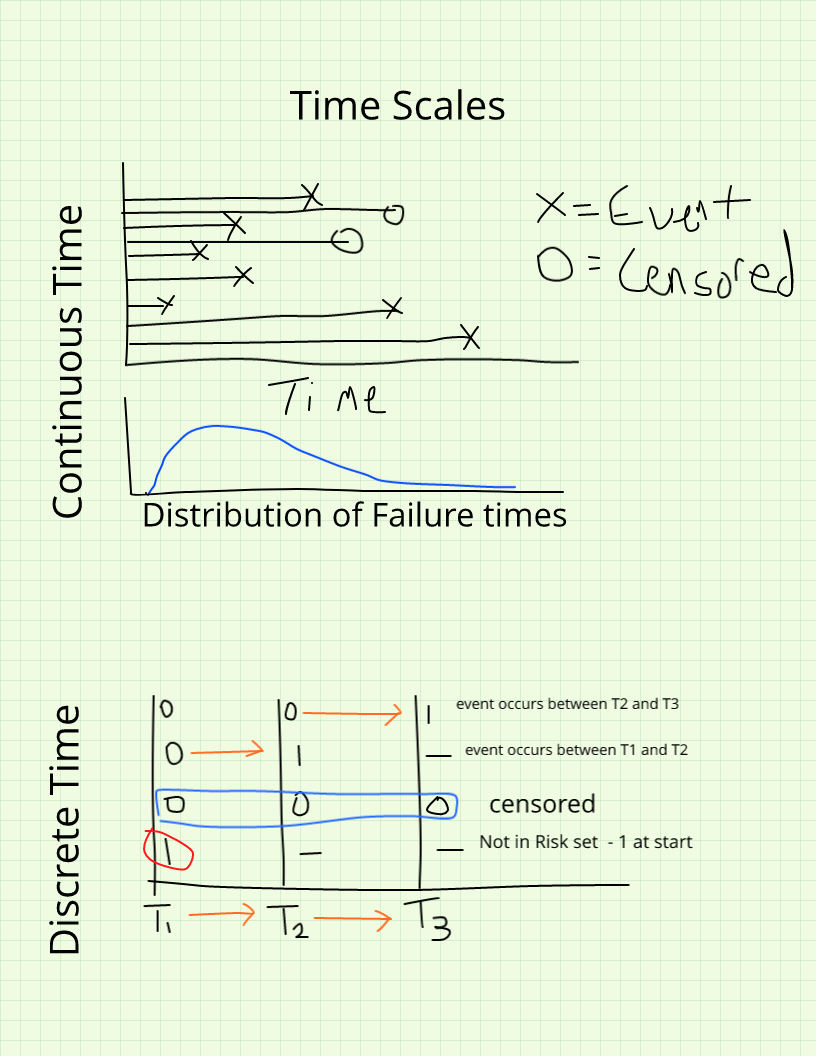
\includegraphics{./images/timescales.png}

}

\caption{Time Scales}

\end{figure}

\hypertarget{making-continuous-outcomes-discrete}{%
\subsubsection{Making continuous outcomes
discrete}\label{making-continuous-outcomes-discrete}}

\begin{itemize}
\item
  Ideally you should measure the duration as finely as possible (see
  Freedman et al)
\item
  Often you may choose to discretize the data \textgreater{} take
  continuous time and break it into discrete chunks
\item
  Problems

  \begin{itemize}
  \tightlist
  \item
    This removes possibly informative information on duration
    variability
  \item
    Any discrete dividing point is arbitrary
  \item
    You may arrive at different conclusions given the interval you
    choose
  \item
    You lose information about late event occurrence
  \item
    Lose all information on mean or average durations
  \end{itemize}
\end{itemize}

\hypertarget{kinds-of-studies-with-event-history-data}{%
\section{Kinds of studies with event history
data}\label{kinds-of-studies-with-event-history-data}}

\begin{itemize}
\item
  Cross sectional

  \begin{itemize}
  \tightlist
  \item
    Measured at one time point (no change observed)
  \item
    Can measure lots of things at once
  \end{itemize}
\item
  Panel data

  \begin{itemize}
  \tightlist
  \item
    Multiple measurements at discrete time points on the same
    individuals
  \item
    Can look at change over time
  \end{itemize}
\item
  Event history

  \begin{itemize}
  \tightlist
  \item
    Continuous measurement of units over a fixed period of time,
    focusing on change in states
  \item
    Think clinical follow-ups
  \end{itemize}
\item
  Longitudinal designs

  \begin{itemize}
  \tightlist
  \item
    Prospective designs
  \item
    Studies that follow a group (cohort) and follow them over time
  \item
    Expensive and take a long time, but can lead to extremely valuable
    information on changes in behaviors
  \end{itemize}
\item
  Retrospective designs
\item
  Taken at a cross section
\item
  Ask respondents about events that have previously occurred.
\item
  Generate birth/migration/marital histories for individuals
\item
  Problems with recall bias
\item
  DHS includes a detailed history of births over the last 5 years
\item
  Record linkage procedures

  \begin{itemize}
  \tightlist
  \item
    Begin with an event of interest (birth, marriage) and follow
    individuals using various record types
  \item
    Birth \textgreater{} Census 1880 \textgreater{} Census 1890
    \textgreater{} Marriage \textgreater{} Birth of children
    \textgreater{} Census 1900 \textgreater{} Tax records
    \textgreater Death certificate
  \item
    Mostly used in historical studies
  \item
    Modern studies link health surveys to National Death Index (NHANES,
    NHIS)
  \end{itemize}
\end{itemize}

\bookmarksetup{startatroot}

\hypertarget{functions-of-survival-time}{%
\chapter{Functions of Survival Time}\label{functions-of-survival-time}}

\hypertarget{some-arrangements-for-event-history-data}{%
\section{Some arrangements for event history
data}\label{some-arrangements-for-event-history-data}}

\hypertarget{counting-process-data}{%
\subsection{Counting process data}\label{counting-process-data}}

\begin{itemize}
\tightlist
\item
  This is what we are accustomed to in the life table
\end{itemize}

\begin{Shaded}
\begin{Highlighting}[]
\NormalTok{t1}\OtherTok{\textless{}{-}}\FunctionTok{data.frame}\NormalTok{(}\AttributeTok{Time\_start=}\FunctionTok{c}\NormalTok{(}\DecValTok{1}\NormalTok{,}\DecValTok{2}\NormalTok{,}\DecValTok{3}\NormalTok{,}\DecValTok{4}\NormalTok{),}
               \AttributeTok{Time\_end=}\FunctionTok{c}\NormalTok{(}\DecValTok{2}\NormalTok{,}\DecValTok{3}\NormalTok{,}\DecValTok{4}\NormalTok{,}\DecValTok{5}\NormalTok{),}
               \AttributeTok{Failing=}\FunctionTok{c}\NormalTok{(}\DecValTok{25}\NormalTok{,}\DecValTok{15}\NormalTok{,}\DecValTok{12}\NormalTok{,}\DecValTok{20}\NormalTok{),}
               \AttributeTok{At\_Risk=}\FunctionTok{c}\NormalTok{(}\DecValTok{100}\NormalTok{, }\DecValTok{75}\NormalTok{, }\DecValTok{60}\NormalTok{, }\DecValTok{40}\NormalTok{))}
\NormalTok{t1}\SpecialCharTok{\%\textgreater{}\%}
  \FunctionTok{kable}\NormalTok{()}\SpecialCharTok{\%\textgreater{}\%}
  \FunctionTok{column\_spec}\NormalTok{(}\DecValTok{1}\SpecialCharTok{:}\DecValTok{4}\NormalTok{, }\AttributeTok{border\_left =}\NormalTok{ T, }\AttributeTok{border\_right =}\NormalTok{ T)}\SpecialCharTok{\%\textgreater{}\%}
  \FunctionTok{kable\_styling}\NormalTok{()}
\end{Highlighting}
\end{Shaded}

\begin{table}
\centering
\begin{tabular}{|>{}r|||>{}r|||>{}r|||>{}r|}
\hline
Time\_start & Time\_end & Failing & At\_Risk\\
\hline
1 & 2 & 25 & 100\\
\hline
2 & 3 & 15 & 75\\
\hline
3 & 4 & 12 & 60\\
\hline
4 & 5 & 20 & 40\\
\hline
\end{tabular}
\end{table}

\begin{Shaded}
\begin{Highlighting}[]
\CommentTok{\#knitr::kable(t1,format = "html", caption = "Counting Process data" ,align = "c", )}
\end{Highlighting}
\end{Shaded}

\hypertarget{case---duration-or-person-level-data}{%
\subsection{Case - duration, or person level
data}\label{case---duration-or-person-level-data}}

\begin{itemize}
\tightlist
\item
  This is the general form of continuous time survival data.
\end{itemize}

\begin{Shaded}
\begin{Highlighting}[]
\NormalTok{t2}\OtherTok{\textless{}{-}}\FunctionTok{data.frame}\NormalTok{(}\AttributeTok{ID =} \FunctionTok{c}\NormalTok{(}\DecValTok{1}\NormalTok{,}\DecValTok{2}\NormalTok{,}\DecValTok{3}\NormalTok{,}\DecValTok{4}\NormalTok{),}
               \AttributeTok{Duration=}\FunctionTok{c}\NormalTok{(}\DecValTok{5}\NormalTok{, }\DecValTok{2}\NormalTok{, }\DecValTok{9}\NormalTok{ , }\DecValTok{6}\NormalTok{), }
               \AttributeTok{Event\_Occurred=}\FunctionTok{c}\NormalTok{(}\StringTok{"Yes (1)"}\NormalTok{,}\StringTok{"Yes (1)"}\NormalTok{,}\StringTok{"No (0)"}\NormalTok{, }\StringTok{"Yes (1)"}\NormalTok{ ))}
\NormalTok{t2}\SpecialCharTok{\%\textgreater{}\%}
  \FunctionTok{kable}\NormalTok{()}\SpecialCharTok{\%\textgreater{}\%}
  \FunctionTok{column\_spec}\NormalTok{(}\DecValTok{1}\SpecialCharTok{:}\DecValTok{3}\NormalTok{, }\AttributeTok{border\_left =}\NormalTok{ T, }\AttributeTok{border\_right =}\NormalTok{ T)}\SpecialCharTok{\%\textgreater{}\%}
  \FunctionTok{kable\_styling}\NormalTok{(}\AttributeTok{row\_label\_position =} \StringTok{"c"}\NormalTok{, }\AttributeTok{position =} \StringTok{"center"}\NormalTok{ )}
\end{Highlighting}
\end{Shaded}

\begin{table}
\centering
\begin{tabular}{|>{}r|||>{}r|||>{}l|}
\hline
ID & Duration & Event\_Occurred\\
\hline
1 & 5 & Yes (1)\\
\hline
2 & 2 & Yes (1)\\
\hline
3 & 9 & No (0)\\
\hline
4 & 6 & Yes (1)\\
\hline
\end{tabular}
\end{table}

\begin{Shaded}
\begin{Highlighting}[]
\CommentTok{\#knitr::kable(t2, format = "html", caption = "Case{-}duration data", align = "c")}
\end{Highlighting}
\end{Shaded}

This can be transformed into person-period data, or discrete time data.

\hypertarget{person-period-data}{%
\subsection{Person -- Period data}\label{person-period-data}}

\begin{itemize}
\tightlist
\item
  Express exposure as discrete periods
\item
  Event occurrence is coded at each period
\end{itemize}

\begin{Shaded}
\begin{Highlighting}[]
\NormalTok{t3}\OtherTok{\textless{}{-}}\FunctionTok{data.frame}\NormalTok{(}\AttributeTok{ID=}\FunctionTok{c}\NormalTok{(}\FunctionTok{rep}\NormalTok{(}\DecValTok{1}\NormalTok{, }\DecValTok{5}\NormalTok{), }\FunctionTok{rep}\NormalTok{(}\DecValTok{2}\NormalTok{, }\DecValTok{2}\NormalTok{), }\FunctionTok{rep}\NormalTok{(}\DecValTok{3}\NormalTok{, }\DecValTok{9}\NormalTok{), }\FunctionTok{rep}\NormalTok{(}\DecValTok{4}\NormalTok{, }\DecValTok{6}\NormalTok{)),}
                    \AttributeTok{Period =} \FunctionTok{c}\NormalTok{(}\FunctionTok{seq}\NormalTok{(}\DecValTok{1}\SpecialCharTok{:}\DecValTok{5}\NormalTok{), }\FunctionTok{seq}\NormalTok{(}\DecValTok{1}\SpecialCharTok{:}\DecValTok{2}\NormalTok{), }\FunctionTok{seq}\NormalTok{(}\DecValTok{1}\SpecialCharTok{:}\DecValTok{9}\NormalTok{), }\FunctionTok{seq}\NormalTok{(}\DecValTok{1}\SpecialCharTok{:}\DecValTok{6}\NormalTok{)),}
                    \AttributeTok{Event=}\FunctionTok{c}\NormalTok{(}\DecValTok{0}\NormalTok{,}\DecValTok{0}\NormalTok{,}\DecValTok{0}\NormalTok{,}\DecValTok{0}\NormalTok{,}\DecValTok{1}\NormalTok{,}\DecValTok{0}\NormalTok{,}\DecValTok{1}\NormalTok{,}\DecValTok{0}\NormalTok{,}\DecValTok{0}\NormalTok{,}\DecValTok{0}\NormalTok{,}\DecValTok{0}\NormalTok{,}\DecValTok{0}\NormalTok{,}\DecValTok{0}\NormalTok{,}\DecValTok{0}\NormalTok{,}\DecValTok{0}\NormalTok{,}\DecValTok{0}\NormalTok{,}\DecValTok{0}\NormalTok{,}\DecValTok{0}\NormalTok{,}\DecValTok{0}\NormalTok{,}\DecValTok{0}\NormalTok{,}\DecValTok{0}\NormalTok{,}\DecValTok{0}\NormalTok{))}
\NormalTok{t3}\SpecialCharTok{\%\textgreater{}\%}
  \FunctionTok{kable}\NormalTok{()}\SpecialCharTok{\%\textgreater{}\%}
  \FunctionTok{column\_spec}\NormalTok{(}\DecValTok{1}\SpecialCharTok{:}\DecValTok{3}\NormalTok{, }\AttributeTok{border\_left =}\NormalTok{ T, }\AttributeTok{border\_right =}\NormalTok{ T)}\SpecialCharTok{\%\textgreater{}\%}
  \FunctionTok{kable\_styling}\NormalTok{(}\AttributeTok{row\_label\_position =} \StringTok{"c"}\NormalTok{, }\AttributeTok{position =} \StringTok{"center"}\NormalTok{ )}
\end{Highlighting}
\end{Shaded}

\begin{table}
\centering
\begin{tabular}{|>{}r|||>{}r|||>{}r|}
\hline
ID & Period & Event\\
\hline
1 & 1 & 0\\
\hline
1 & 2 & 0\\
\hline
1 & 3 & 0\\
\hline
1 & 4 & 0\\
\hline
1 & 5 & 1\\
\hline
2 & 1 & 0\\
\hline
2 & 2 & 1\\
\hline
3 & 1 & 0\\
\hline
3 & 2 & 0\\
\hline
3 & 3 & 0\\
\hline
3 & 4 & 0\\
\hline
3 & 5 & 0\\
\hline
3 & 6 & 0\\
\hline
3 & 7 & 0\\
\hline
3 & 8 & 0\\
\hline
3 & 9 & 0\\
\hline
4 & 1 & 0\\
\hline
4 & 2 & 0\\
\hline
4 & 3 & 0\\
\hline
4 & 4 & 0\\
\hline
4 & 5 & 0\\
\hline
4 & 6 & 0\\
\hline
\end{tabular}
\end{table}

\hypertarget{homage-to-the-life-table}{%
\section{Homage to the life table}\label{homage-to-the-life-table}}

In life tables, we had lots of functions of the death process. Some of
these were more interesting than others, with two being of special
interest to use here. These are the \(l(x)\) and \(q(x, n)\) functions.
If you recall, \(l(x)\) represents the population size of the stationary
population that is alive at age \(x\), and the risk of dying between age
\(x, x+n\) is \(q(x, n)\).

These are genearlized more in the event history analysis literature, but
we can still describe the distrubion of survival time using three
functions. These are the \textbf{Survival Function}, \(S(t)\), the
\textbf{probability density function}, \(f(t)\), and the \textbf{hazard
function}, \(h(t)\). These three are related and we can derive one from
the others.

Now we must generalize these ideas to incorporate them into the broader
event-history framework

Survival/duration times measure the \emph{time to a certain event.}

These times are subject to random variations, and are considered to be
random \emph{iid} (independent and identically distributed; random)
variates from some distribution

\begin{itemize}
\tightlist
\item
  The distribution of survival times is described by 3 functions
\item
  The survivorship function, \(S(t)\)
\item
  The probability density function, \(f(t)\)
\item
  The hazard function, \(h(t)\)
\end{itemize}

\begin{figure}

{\centering \includegraphics{C:/Users/ozd504/Documents/GitHub/DEM7223/images/functions.png}

}

\caption{3 functions}

\end{figure}

\begin{Shaded}
\begin{Highlighting}[]
\NormalTok{Ft}\OtherTok{\textless{}{-}}\FunctionTok{cumsum}\NormalTok{(}\FunctionTok{dlnorm}\NormalTok{(}\AttributeTok{x =} \FunctionTok{seq}\NormalTok{(}\DecValTok{0}\NormalTok{, }\DecValTok{110}\NormalTok{, }\DecValTok{1}\NormalTok{), }\AttributeTok{meanlog =} \FloatTok{4.317488}\NormalTok{, }\AttributeTok{sdlog =} \FloatTok{2.5}\NormalTok{)) }\CommentTok{\#mean of 75 years, sd of 12.1 years}
\NormalTok{ft}\OtherTok{\textless{}{-}}\FunctionTok{diff}\NormalTok{(Ft)}
\NormalTok{St}\OtherTok{\textless{}{-}}\DecValTok{1}\SpecialCharTok{{-}}\NormalTok{Ft}
\NormalTok{ht}\OtherTok{\textless{}{-}}\NormalTok{ft}\SpecialCharTok{/}\NormalTok{St[}\DecValTok{1}\SpecialCharTok{:}\DecValTok{110}\NormalTok{]}
\FunctionTok{plot}\NormalTok{(Ft, }\AttributeTok{ylim=}\FunctionTok{c}\NormalTok{(}\DecValTok{0}\NormalTok{,}\DecValTok{1}\NormalTok{))}
\FunctionTok{lines}\NormalTok{(St, }\AttributeTok{col=}\StringTok{"red"}\NormalTok{)}
\end{Highlighting}
\end{Shaded}

\begin{figure}[H]

{\centering 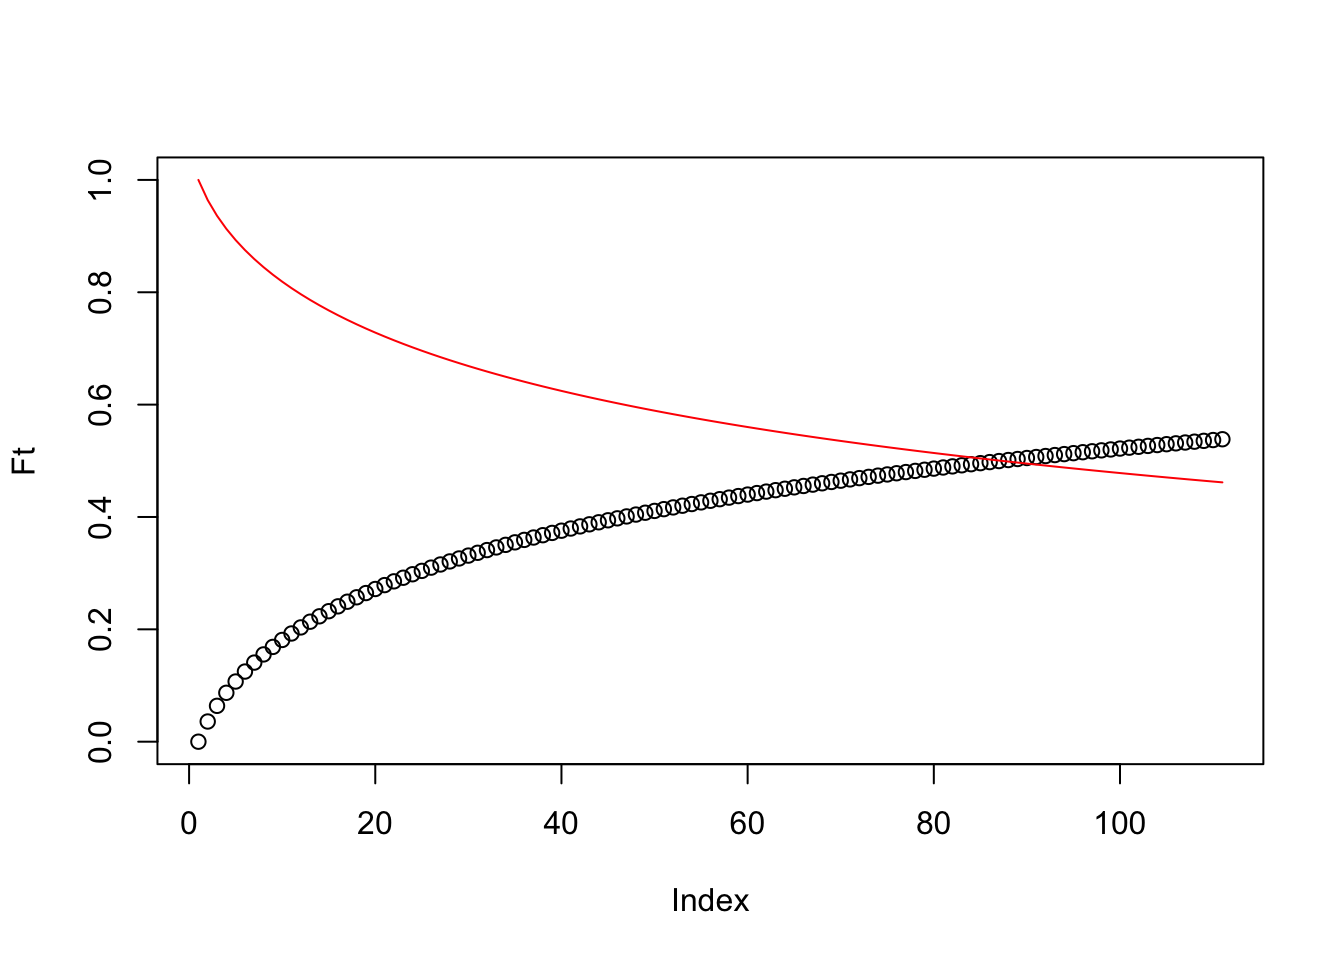
\includegraphics{micro_files/figure-pdf/unnamed-chunk-5-1.pdf}

}

\end{figure}

\begin{Shaded}
\begin{Highlighting}[]
\FunctionTok{plot}\NormalTok{(ht, }\AttributeTok{col=}\StringTok{"green"}\NormalTok{)}
\end{Highlighting}
\end{Shaded}

\begin{figure}[H]

{\centering 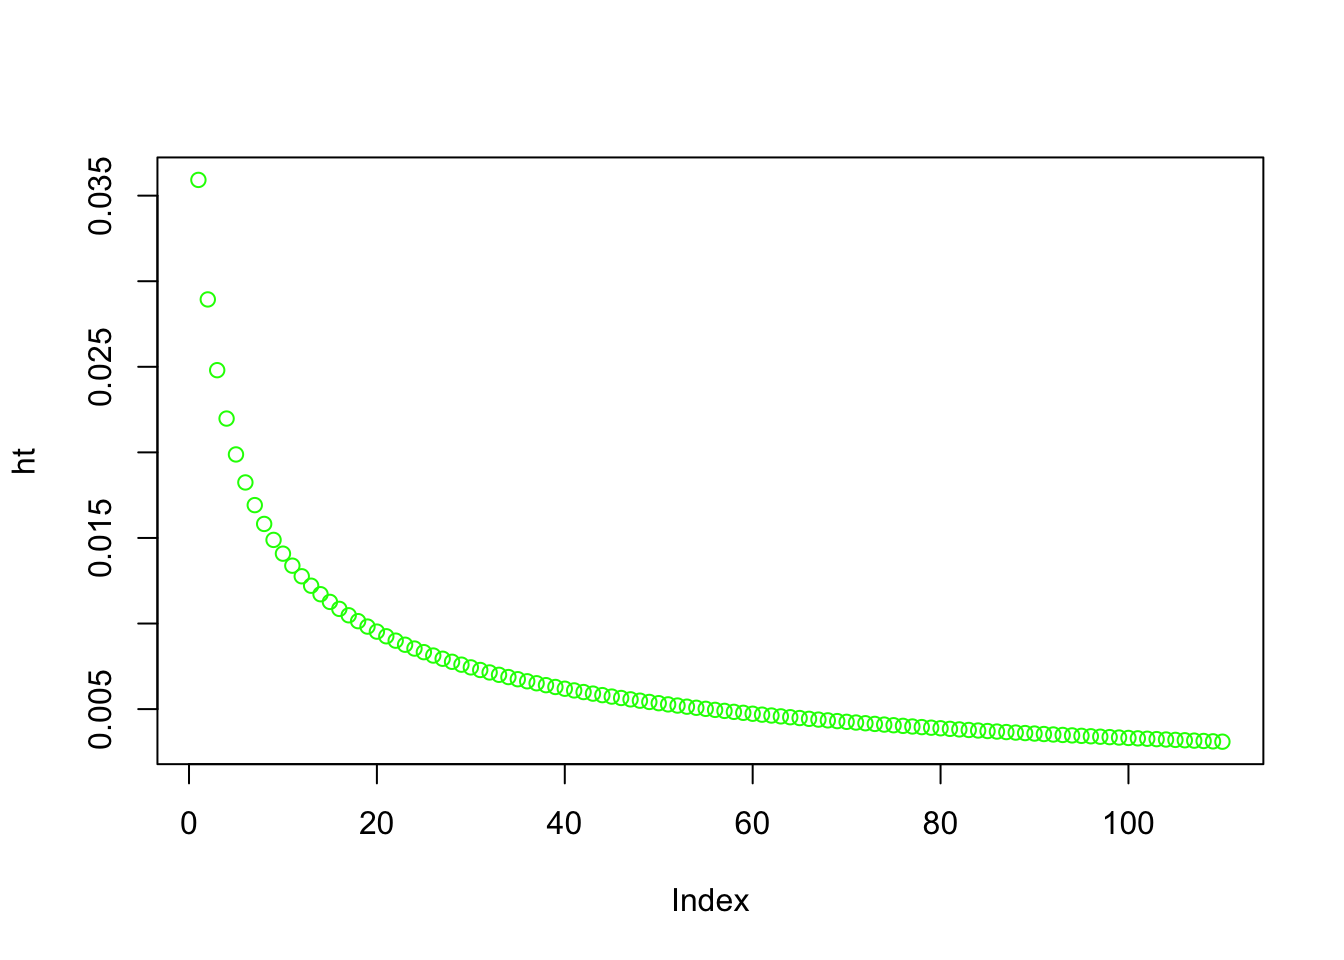
\includegraphics{micro_files/figure-pdf/unnamed-chunk-5-2.pdf}

}

\end{figure}

\begin{itemize}
\tightlist
\item
  These three are mathematically related, and if given one, we can
  calculate the others

  \begin{itemize}
  \tightlist
  \item
    These 3 functions each represent a different aspect of the survival
    time distribution.
  \end{itemize}
\item
  The fundamental problem in survival analysis is coming up with a way
  to estimate these functions.
\end{itemize}

\hypertarget{defining-the-functions}{%
\subsection{Defining the functions}\label{defining-the-functions}}

Let \emph{T} denote the survival time, our goal is to characterize the
distribution of \emph{T} using these 3 functions.

Let \emph{T} be a discrete(or continuous) \emph{iid} random variable and
let \(t_i\), be an occurrence of that variable, such that
\(Pr(t_i)=Pr(T=t_i)\)

\hypertarget{the-distribution-function-or-pdf}{%
\subsection{\texorpdfstring{The distribution function, or
\emph{pdf}}{The distribution function, or pdf}}\label{the-distribution-function-or-pdf}}

Like any other random variates survival times have a simple distribution
function that gives the probability of observing a particular survival
time within a finite interval

The density function is defined as the limit of the probability that an
individual fails (experiences the event) in a short interval
\(t+\Delta t\) (read delta t), per width of \(\Delta t\), or simply the
probability of failure in a small interval per unit time,
\(f(t_i) = Pr(T=t_i)\).

If \(F(t)\) is the cumulative distribution function for \emph{T}, given
by:

\[ F(t) = \int_{0}^{t} f(u) du = Pr(T \leqslant t )\] Which is the
probability of observing a value of \emph{T} prior to the current value,
\emph{t}.

The density function is then:

\[ f(t) = \frac{F(t)}{d(t)} = F'(t)\] or

\[ f(t) = \lim_{\delta t \rightarrow 0} \frac{F(t+\Delta t) - F(t)}{\Delta t}\]

The density function gives the unconditional instantaneous failure rate
in the (very small) interval between \emph{t} and \emph{dt},
\(\Delta t\)

\hypertarget{survival-function}{%
\subsection{Survival Function}\label{survival-function}}

The survival function, \emph{S(t)} is expressed:

\[ S(t) = 1 - F(t) = Pr (T \geqslant t)\]

Which is the probability that \emph{T} takes a value larger than
\emph{t}. i.e.~the event happens some time after the present time.

At \(t = 0, S(t) =1 \text { and at } t= \infty, \text { and } S(t) =0\)

As time passes, \emph{S(t)} decreases, and is called a \emph{strictly
decreasing function of time}.

Empirically, \emph{S(t)} takes the form of a step function:

\begin{Shaded}
\begin{Highlighting}[]
\NormalTok{St}\OtherTok{\textless{}{-}} \FunctionTok{c}\NormalTok{(}\DecValTok{1}\NormalTok{, }\FunctionTok{cumprod}\NormalTok{(}\DecValTok{1}\SpecialCharTok{{-}}\NormalTok{(t1}\SpecialCharTok{$}\NormalTok{Failing}\SpecialCharTok{/}\NormalTok{t1}\SpecialCharTok{$}\NormalTok{At\_Risk)))}

\FunctionTok{plot}\NormalTok{(St, }\AttributeTok{type=}\StringTok{"s"}\NormalTok{, }\AttributeTok{xlab =} \StringTok{"Time"}\NormalTok{, }\AttributeTok{ylab=}\StringTok{"S(t)"}\NormalTok{, }\AttributeTok{ylim=}\FunctionTok{c}\NormalTok{(}\DecValTok{0}\NormalTok{,}\DecValTok{1}\NormalTok{))}
\end{Highlighting}
\end{Shaded}

\begin{figure}[H]

{\centering \includegraphics{micro_files/figure-pdf/unnamed-chunk-6-1.pdf}

}

\end{figure}

\hypertarget{the-hazard-function}{%
\subsection{The hazard function}\label{the-hazard-function}}

The hazard function relates death, \emph{f(t)}, and survival,
\emph{S(t)}, to one another

\[h(t) = \frac{f(t)}{S(t)}\]
\[h(t) = \lim_{\Delta t \rightarrow 0} \frac{Pr(t \leqslant T \leqslant t + \Delta t | T \geqslant t)}{\Delta t}\]

Which is the failure rate per unit time in the interval \emph{t},
\(t+\Delta t\), the hazard may increase or decrease with time, or stay
the same. This is really dependent on the distribution of failure times.

\hypertarget{relationships-among-the-three-functions}{%
\section{Relationships among the three
functions}\label{relationships-among-the-three-functions}}

If \(ft = \frac{dF(t)}{dt}\) and \(S(t) = 1- F(t)\) and,
\(h(t) = \frac{f(t)}{S(t)}\), then we can write:

\[f(t) = \frac{-dS(t)}{dt}\]

and the hazard function as:

\[h(t) = \frac{-d \text{ log } S(t)}{dt}\]

If we integrate this and let \(S(0)=1\), then

\[S(t) = exp^{-\int_{0}^t h(u) du} = e^{-H(t)}\]

where the quantity, \(H(t)\) is called the \emph{cumulative hazard
function} and, \(H(t) = \int h(u) du\), then

\[H(t) = -\text{log }  S(t)\]

The density can be written as:

\[f(t) = h(t) e ^{-H(t)}\] and

\[h(t) = \frac{h(t) e^{-H(t)}}{e^{-H(t)}} = \frac{f(t)}{S(t)}\]

\hypertarget{more-on-the-hazard-function}{%
\subsection{More on the hazard
function\ldots{}}\label{more-on-the-hazard-function}}

Unlike the \emph{f(t)} or \emph{S(t)}, \emph{h(t)} describes the risk an
individual faces of experiencing the event, given they have survived up
to that time.

This kind of conditional probability is of special interest to us.

We can extend this framework to include effects of \emph{individual
characteristics on one's risk}, thus not only introducing dependence on
time, but also on these characteristics (covariates).

We can re-express the hazard rate with both these conditions as:

\[h(t|x) = \lim_{\Delta t \rightarrow 0} \frac{Pr(t \leqslant T \leqslant t + \Delta t | T \geqslant t, x)}{\Delta t}\]
\#\# Logistic regression When a variable is coded as binary, meaning
either 1 or 0, the Bernoulli distribution is used, as in the logistic
regression model. When coded like this, the model tries to use the other
measured information to predict the 1 value versus the 0 value. So in
the basic sense, we want to construct a model like:

\[Pr(y=1) =\pi =  \text{some function of predictors}\]

\hypertarget{refs}{}
\begin{CSLReferences}{1}{0}
\leavevmode\vadjust pre{\hypertarget{ref-anselin_spatial_1988}{}}%
Anselin, Luc. 1988. \emph{Spatial {Econometrics}: {Methods} and
{Models}.} Dordrecht: Springer Netherlands.

\leavevmode\vadjust pre{\hypertarget{ref-breslow_extra-poisson_1984}{}}%
Breslow, N. E. 1984. {``Extra-{Poisson} {Variation} in {Log}-{Linear}
{Models}.''} \emph{Applied Statistics} 33 (1): 38.
\url{https://doi.org/10.2307/2347661}.

\leavevmode\vadjust pre{\hypertarget{ref-us_census_bureau_worked_nodate}{}}%
Bureau, US Census. 2019. {``Worked {Examples} for {Approximating}
{Standard} {Errors} {Using} {American} {Community} {Survey} {Data}.''}
\url{https://www2.census.gov/programs-surveys/acs/tech_docs/accuracy/2018_ACS_Accuracy_Document_Worked_Examples.pdf}.

\leavevmode\vadjust pre{\hypertarget{ref-cameron_practitioners_2015}{}}%
Cameron, A. Colin, and Douglas L. Miller. 2015. {``A {Practitioner}'s
{Guide} to {Cluster}-{Robust} {Inference}.''} \emph{Journal of Human
Resources} 50 (2): 317--72. \url{https://doi.org/10.3368/jhr.50.2.317}.

\leavevmode\vadjust pre{\hypertarget{ref-cdc2020}{}}%
CDC. 2020. {``Weighting the BRFSS Data.''}
\url{https://www.cdc.gov/brfss/annual_data/2019/pdf/weighting-2019-508.pdf}.

\leavevmode\vadjust pre{\hypertarget{ref-chi_spatial_2020}{}}%
Chi, Guangqing, and Jun Zhu. 2020. \emph{Spatial Regression Models for
the Social Sciences}. Los Angeles: SAGE.

\leavevmode\vadjust pre{\hypertarget{ref-courtemanche2019}{}}%
Courtemanche, Charles, James Marton, Benjamin Ukert, Aaron Yelowitz, and
Daniela Zapata. 2019. {``Effects of the Affordable Care Act on Health
Behaviors After 3~Years.''} \emph{Eastern Economic Journal} 45 (1):
7--33. \url{https://doi.org/10.1057/s41302-018-0119-4}.

\leavevmode\vadjust pre{\hypertarget{ref-cribari-neto_beta_2010}{}}%
Cribari-Neto, Francisco, and Achim Zeileis. 2010. {``Beta {Regression}
in \emph{r}.''} \emph{Journal of Statistical Software} 34 (2).
\url{https://doi.org/10.18637/jss.v034.i02}.

\leavevmode\vadjust pre{\hypertarget{ref-united_nations_population_division_manual_1983}{}}%
Division, United Nations Population. 1983. {``Manual {X}: {Indirect}
{Techniques} for {Demographic} {Estimation}.''} New York, NY.
\url{https://www.un.org/en/development/desa/population/publications/manual/estimate/demographic-estimation.asp}.

\leavevmode\vadjust pre{\hypertarget{ref-elhorst_spatial_2014}{}}%
Elhorst, J. Paul. 2014. \emph{Spatial {Econometrics}: {From}
{Cross}-{Sectional} {Data} to {Spatial} {Panels}}. 1st ed. 2014.
{SpringerBriefs} in {Regional} {Science}. Berlin, Heidelberg: Springer
Berlin Heidelberg : Imprint: Springer.
\url{https://doi.org/10.1007/978-3-642-40340-8}.

\leavevmode\vadjust pre{\hypertarget{ref-entwisle_2007}{}}%
Entwisle, Barbara. 2007. {``Putting People into Place.''}
\emph{Demography} 44 (4): 687--703.
\url{https://doi.org/10.1353/dem.2007.0045}.

\leavevmode\vadjust pre{\hypertarget{ref-fox_applied_2016}{}}%
Fox, John. 2016. \emph{Applied Regression Analysis and Generalized
Linear Models}. Third Edition. Los Angeles: SAGE.

\leavevmode\vadjust pre{\hypertarget{ref-betareg}{}}%
Grün, Bettina, Ioannis Kosmidis, and Achim Zeileis. 2012. {``Extended
Beta Regression in {R}: Shaken, Stirred, Mixed, and Partitioned.''}
\emph{Journal of Statistical Software} 48 (11): 1--25.
\url{https://doi.org/10.18637/jss.v048.i11}.

\leavevmode\vadjust pre{\hypertarget{ref-stargazer}{}}%
Hlavac, Marek. 2018. \emph{Stargazer: Well-Formatted Regression and
Summary Statistics Tables}. Bratislava, Slovakia: Central European
Labour Studies Institute (CELSI).
\url{https://CRAN.R-project.org/package=stargazer}.

\leavevmode\vadjust pre{\hypertarget{ref-GT}{}}%
Iannone, Richard, Joe Cheng, and Barret Schloerke. 2020. \emph{Gt:
Easily Create Presentation-Ready Display Tables}.
\url{https://CRAN.R-project.org/package=gt}.

\leavevmode\vadjust pre{\hypertarget{ref-Iannone2021}{}}%
---------. 2021. \emph{Gt: Easily Create Presentation-Ready Display
Tables}. \url{https://CRAN.R-project.org/package=gt}.

\leavevmode\vadjust pre{\hypertarget{ref-ibragimov_inference_2016}{}}%
Ibragimov, Rustam, and Ulrich K. Müller. 2016. {``Inference with {Few}
{Heterogeneous} {Clusters}.''} \emph{The Review of Economics and
Statistics} 98 (1): 83--96. \url{https://doi.org/10.1162/REST_a_00545}.

\leavevmode\vadjust pre{\hypertarget{ref-international_demographic_2012}{}}%
International, ICF. 2012. {``Demographic and {Health} {Survey}
{Sampling} and {Household} {Listing} {Manual}.''} ICF International.

\leavevmode\vadjust pre{\hypertarget{ref-keyfitz_introduction_1968}{}}%
Keyfitz, Nathan. 1968. \emph{Introduction to the {Mathematics} of
{Population}}. Addison-Wesley Publishing Company.

\leavevmode\vadjust pre{\hypertarget{ref-kleinman}{}}%
Kleinman, Ken, and Nicholas J. Horton. 2014. \emph{SAS and r: Data
Management, Statistical Analysis, and Graphics, 2nd Edition}. 2nd ed.
Boca Raton, Florida: Chapman; Hall/CRC.
\url{https://nhorton.people.amherst.edu/sasr2/}.

\leavevmode\vadjust pre{\hypertarget{ref-lesage_introduction_2009}{}}%
LeSage, James P., and R. Kelley Pace. 2009. \emph{Introduction to
Spatial Econometrics}. Statistics, Textbooks and Monographs. Boca Raton:
CRC Press.

\leavevmode\vadjust pre{\hypertarget{ref-Lohr2019}{}}%
Lohr, Shron. 2019. \emph{Sampling: Design and Analysis}. 2nd ed. Boca
Raton: Routledg/CRC Press.

\leavevmode\vadjust pre{\hypertarget{ref-long_using_2000}{}}%
Long, J. Scott, and Laurie H. Ervin. 2000. {``Using {Heteroscedasticity}
{Consistent} {Standard} {Errors} in the {Linear} {Regression}
{Model}.''} \emph{The American Statistician} 54 (3): 217--24.
\url{https://doi.org/10.1080/00031305.2000.10474549}.

\leavevmode\vadjust pre{\hypertarget{ref-lumley2004}{}}%
Lumley, Thomas. 2004. {``Analysis of Complex Survey Samples.''}
\emph{Journal of Statistical Software} 9 (1): 1--19.

\leavevmode\vadjust pre{\hypertarget{ref-lumley2010}{}}%
---------. 2010. \emph{Complex {Surveys}: {A} {Guide} to {Analysis}
{Using} {R}: {A} {Guide} to {Analysis} {Using} {R}}. John Wiley; Sons.

\leavevmode\vadjust pre{\hypertarget{ref-lumleysvyvgam}{}}%
---------. 2021. \emph{svyVGAM: Design-Based Inference in Vector
Generalised Linear Models}.
\url{https://CRAN.R-project.org/package=svyVGAM}.

\leavevmode\vadjust pre{\hypertarget{ref-mackinnon_white_1985}{}}%
MacKinnon, James G, and Halbert White. 1985. {``Some
Heteroskedasticity-Consistent Covariance Matrix Estimators with Improved
Finite Sample Properties.''} \emph{Journal of Econometrics} 29 (3):
305--25. \url{https://doi.org/10.1016/0304-4076(85)90158-7}.

\leavevmode\vadjust pre{\hypertarget{ref-nhgis}{}}%
Manson, Steven, Jonathan Schroeder, David Van Riper, Tracy Kugler, and
Steven Ruggles. 2021. \emph{IPUMS National Historical Geographic
Information System: Version 16.0 {[}Dataset{]}}.
https://doi.org/\url{http://doi.org/10.18128/D050.V16.0}.

\leavevmode\vadjust pre{\hypertarget{ref-mccullagh_generalized_1998}{}}%
McCullagh, P., and John A. Nelder. 1998. \emph{Generalized Linear
Models}. 2nd ed. Monographs on Statistics and Applied Probability 37.
Boca Raton: Chapman \& Hall/CRC.

\leavevmode\vadjust pre{\hypertarget{ref-mclaughlin_differential_2007}{}}%
McLaughlin, Diane K., C. Shannon Stokes, P. Johnelle Smith, and A
Nonoyama. 2007. {``Differential Mortality Across the {United} {States}:
The Influence of Place-Based Inequality.''} In \emph{Sociology of
{Spatial} {Inequality}}, 141--62. State University of New York Press.

\leavevmode\vadjust pre{\hypertarget{ref-nelder_generalized_1972}{}}%
Nelder, J. A., and R. W. M. Wedderburn. 1972. {``Generalized {Linear}
{Models}.''} \emph{Journal of the Royal Statistical Society: Series A
(General)} 135 (3): 370--84. \url{https://doi.org/10.2307/2344614}.

\leavevmode\vadjust pre{\hypertarget{ref-pinheiro_mixed-effects_2000}{}}%
Pinheiro, José C., and Douglas M. Bates. 2000. \emph{Mixed-Effects
Models in {S} and {S}-{PLUS}}. Statistics and Computing. New York:
Springer.

\leavevmode\vadjust pre{\hypertarget{ref-rao_chi-squared_1984}{}}%
Rao, JNK, and AJ Scott. 1984. {``On {Chi}-Squared {Tests} {For}
{Multiway} {Contigency} {Tables} with {Proportions} {Estimated} {From}
{Survey} {Data}.''} \emph{Annals of Statistics} 12: 46--60.

\leavevmode\vadjust pre{\hypertarget{ref-gamlss}{}}%
Rigby, R. A., and D. M. Stasinopoulos. 2005. {``Generalized Additive
Models for Location, Scale and Shape,(with Discussion).''} \emph{Applied
Statistics} 54.3: 507--54.

\leavevmode\vadjust pre{\hypertarget{ref-Ruggles2021}{}}%
Ruggles, S, S Flood, Josiah Grover, S Foster, R Goeken, Jose Pacas, Erin
Schouweiler, and M Sobek. 2021. {``Integrated {Public} {Use} {Microdata}
{Series}: {Version} 11.0 {[}Machine-Readable Database{]}.''}
https://doi.org/\url{https://doi.org/10.18128/D010.V8.0}.

\leavevmode\vadjust pre{\hypertarget{ref-gtsummary}{}}%
Sjoberg, Daniel D., Karissa Whiting, Michael Curry, Jessica A. Lavery,
and Joseph Larmarange. 2021. {``Reproducible Summary Tables with the
Gtsummary Package.''} \emph{{The R Journal}} 13: 570--80.
\url{https://doi.org/10.32614/RJ-2021-053}.

\leavevmode\vadjust pre{\hypertarget{ref-soni2017a}{}}%
Soni, Aparna, Michael Hendryx, and Kosali Simon. 2017. {``Medicaid
Expansion Under the Affordable Care Act and Insurance Coverage in Rural
and Urban Areas.''} \emph{The Journal of Rural Health} 33 (2): 217--26.
\url{https://doi.org/10.1111/jrh.12234}.

\leavevmode\vadjust pre{\hypertarget{ref-sparks_application_2010}{}}%
Sparks, Patrice Johnelle, and Corey S. Sparks. 2010. {``An Application
of Spatially Autoregressive Models to the Study of {US} County Mortality
Rates: {An} {Application} of {Spatially} {Autoregressive} {Models}.''}
\emph{Population, Space and Place} 16 (6): 465--81.
\url{https://doi.org/10.1002/psp.564}.

\leavevmode\vadjust pre{\hypertarget{ref-uscensusbureau2014}{}}%
US Census Bureau. 2014. {``American Community Survey Design and
Methodology (January 2014).''}
\url{https://www2.census.gov/programs-surveys/acs/methodology/design_and_methodology/acs_design_methodology_report_2014.pdf}.

\leavevmode\vadjust pre{\hypertarget{ref-venables_ripley}{}}%
Venables, W. N., and B. D. Ripley. 2002. \emph{Modern Applied Statistics
with s}. Fourth. New York: Springer.
\url{https://www.stats.ox.ac.uk/pub/MASS4/}.

\leavevmode\vadjust pre{\hypertarget{ref-voss_demography_2007}{}}%
Voss, Paul R. 2007. {``Demography as a {Spatial} {Social} {Science}.''}
\emph{Population Research and Policy Review} 26 (5-6): 457--76.
\url{https://doi.org/10.1007/s11113-007-9047-4}.

\leavevmode\vadjust pre{\hypertarget{ref-tigris}{}}%
Walker, Kyle. 2021. \emph{Tigris: Load Census TIGER/Line Shapefiles}.
\url{https://CRAN.R-project.org/package=tigris}.

\leavevmode\vadjust pre{\hypertarget{ref-walker21}{}}%
Walker, Kyle, and Matt Herman. 2021. \emph{Tidycensus: Load US Census
Boundary and Attribute Data as 'Tidyverse' and 'Sf'-Ready Data Frames}.
\url{https://CRAN.R-project.org/package=tidycensus}.

\leavevmode\vadjust pre{\hypertarget{ref-rdhs}{}}%
Watson, Oliver J, Rich FitzJohn, and Jeffrey W Eaton. 2019. {``Rdhs: An
r Package to Interact with the Demographic and Health Surveys (DHS)
Program Datasets.''} \emph{Wellcome Open Research} 4: 103.
\url{https://doi.org/10.12688/wellcomeopenres.15311.1}.

\leavevmode\vadjust pre{\hypertarget{ref-white_1980}{}}%
White, Halbert. 1980. {``A {Heteroskedasticity}-{Consistent}
{Covariance} {Matrix} {Estimator} and a {Direct} {Test} for
{Heteroskedasticity}.''} \emph{Econometrica} 48 (4): 817.
\url{https://doi.org/10.2307/1912934}.

\leavevmode\vadjust pre{\hypertarget{ref-ggplot2}{}}%
Wickham, Hadley. 2016. \emph{Ggplot2: Elegant Graphics for Data
Analysis}. Springer-Verlag New York.
\url{https://ggplot2.tidyverse.org}.

\leavevmode\vadjust pre{\hypertarget{ref-Wickham}{}}%
---------. n.d. \emph{{R Packages}}. 1st ed. O'Reily.
\url{https://r-pkgs.org/}.

\leavevmode\vadjust pre{\hypertarget{ref-tidyverse}{}}%
Wickham, Hadley, Mara Averick, Jennifer Bryan, Winston Chang, Lucy
D'Agostino McGowan, Romain François, Garrett Grolemund, et al. 2019.
{``Welcome to the {tidyverse}.''} \emph{Journal of Open Source Software}
4 (43): 1686. \url{https://doi.org/10.21105/joss.01686}.

\leavevmode\vadjust pre{\hypertarget{ref-dplyr}{}}%
Wickham, Hadley, Romain François, Lionel Henry, and Kirill Müller. 2020.
\emph{Dplyr: A Grammar of Data Manipulation}.
\url{https://CRAN.R-project.org/package=dplyr}.

\leavevmode\vadjust pre{\hypertarget{ref-Wickham2017R}{}}%
Wickham, Hadley, and Garrett Grolemund. 2017. \emph{R for Data Science:
Import, Tidy, Transform, Visualize, and Model Data}. 1st ed. Paperback;
O'Reilly Media. \url{http://r4ds.had.co.nz/}.

\leavevmode\vadjust pre{\hypertarget{ref-haven}{}}%
Wickham, Hadley, and Evan Miller. 2020. \emph{Haven: Import and Export
'SPSS', 'Stata' and 'SAS' Files}.
\url{https://CRAN.R-project.org/package=haven}.

\end{CSLReferences}



\end{document}
